\documentclass[utf8]{frontiersSCNS} % for Science, Engineering and Humanities and Social Sciences articles
%\documentclass[utf8]{frontiersHLTH} % for Health articles
%\documentclass[utf8]{frontiersFPHY} % for Physics and Applied Mathematics and Statistics articles
%\setcitestyle{square} % for Physics and Applied Mathematics and Statistics articles
\usepackage[french]{babel}
\usepackage{url,hyperref,lineno,microtype,subcaption}
\usepackage[onehalfspacing]{setspace}
\usepackage[toc,page]{appendix} 
\usepackage{pdfpages}
\usepackage{color, colortbl}
\usepackage{multirow}
\linenumbers


% Leave a blank line between paragraphs instead of using \\


\def\keyFont{\fontsize{8}{11}\helveticabold }
\def\firstAuthorLast{Dermy {et~al.}} %use et al only if is more than 1 author
\def\Authors{Oriane Dermy\,$^{1,*}$, Alexandros Paraschos\,$^{2,4}$, Marco Ewerton\,$^{2}$,  Jan Peters\,$^{2,3}$, Fran\c cois Charpillet\,$^{1}$ and Serena Ivaldi\,$^{1}$}
% Affiliations should be keyed to the author's name wifth superscript numbers and be listed as follows: Laboratory, Institute, Department, Organisation, City, State abbreviation (USA, Canada, Australia), and Country (without detailed address information such as city zip codes or street names).
% If one of the authors has a change of address, list the new address below the correspondence details using a superscript symbol and use the same symbol to indicate the author in the author list.
\def\Address{$^{1}$ Inria, Villers-lés-Nancy, 54600, France; \\Université de Lorraine, Loria, UMR7503, Vandoeuvre, 54500, France; \\
CNRS, Loria, UMR7503, Vandoeuvre, 54500, France \\
        {\tt\small name.surname@inria.fr}\\
$^{2}$TU Darmstadt, Darmstadt, Germany\\
$^{3}$Max Planck Institute for Intelligent Systems, Tubingen, Germany\\
$^{4}$Data Lab, Volkswagen Group, 80805 Munich, Germany}
% The Corresponding Author should be marked with an asterisk
% Provide the exact contact address (this time including street name and city zip code) and email of the corresponding author
\def\corrAuthor{Corresponding Author}

\def\corrEmail{oriane.dermy@inria.fr}


%%%% PACKAGES %%%%
%
%% The following packages can be found on http:\\www.ctan.org
%\usepackage{graphics} % for pdf, bitmapped graphics files
%%\usepackage{epsfig} % for postscript graphics files
%%\usepackage{mathptmx} % assumes new font selection scheme installed
%%\usepackage{times} % assumes new font selection scheme installed
%%\usepackage{amsmath} % assumes amsmath package installed
%%\usepackage{amssymb}  % assumes amsmath package installed
%
%% *** MATH PACKAGES ***
%%
%\usepackage{amsmath}
%% A popular package from the American Mathematical Society that provides
%% many useful and powerful commands for dealing with mathematics.
%%
%% Note that the amsmath package sets \interdisplaylinepenalty to 10000
%% thus preventing page breaks from occurring within multiline equations. Use:
%%\interdisplaylinepenalty=2500
%% after loading amsmath to restore such page breaks as IEEEtran.cls normally
%% does. amsmath.sty is already installed on most LaTeX systems. The latest
%% version and documentation can be obtained at:
%% http://www.ctan.org/pkg/amsmath
%\usepackage{amssymb}  % assumes amsmath package installed
%\usepackage{bm} 
\usepackage{dsfont}

%\usepackage{bbm}
%\usepackage{bbold}
%
%% *** SPECIALIZED LIST PACKAGES ***
%%
%%\usepackage{algorithmic}
%% algorithmic.sty was written by Peter Williams and Rogerio Brito.
%% This package provides an algorithmic environment fo describing algorithms.
%% You can use the algorithmic environment in-text or within a figure
%% environment to provide for a floating algorithm. Do NOT use the algorithm
%% floating environment provided by algorithm.sty (by the same authors) or
%% algorithm2e.sty (by Christophe Fiorio) as the IEEE does not use dedicated
%% algorithm float types and packages that provide these will not provide
%% correct IEEE style captions. The latest version and documentation of
%% algorithmic.sty can be obtained at:
%% http://www.ctan.org/pkg/algorithms
%% Also of interest may be the (relatively newer and more customizable)
%% algorithmicx.sty package by Szasz Janos:
%% http://www.ctan.org/pkg/algorithmicx
%\usepackage{algorithm}
%\usepackage{algpseudocode}
%\usepackage{tcolorbox}
%\usepackage{tikz}
%
%% *** PDF, URL AND HYPERLINK PACKAGES ***
%%
%\usepackage{url}
%% url.sty was written by Donald Arseneau. It provides better support for
%% handling and breaking URLs. url.sty is already installed on most LaTeX
%% systems. The latest version and documentation can be obtained at:
%% http://www.ctan.org/pkg/url
%% Basically, \url{my_url_here}.

% https://fr.mathworks.com/matlabcentral/fileexchange/8015-m-code-latex-package
% load package with some of the available options (default by template)
\usepackage[framed,numbered,autolinebreaks,useliterate]{mcode}
 \usepackage{ulem}

\newcommand{\rev}[1]{\textcolor{blue}{#1}}
\newcommand{\ori}[1]{\textcolor{teal}{#1}}


\newcommand{\toimprove}[1]{\textcolor{teal}{#1}}
\newcommand{\todo}[1]{\textcolor{red}{\textbf{/*#1*/}}}
\newcommand{\quest}[1]{\textcolor{green}{\textit{#1}}}

\newcommand*\rfrac[2]{{}^{#1}\!/_{#2}}

% pick one of these colors
%black, blue, brown, cyan, darkgray, gray, green, lightgray, lime, magenta, olive, orange, pink, purple, red, teal, violet, white, yellow.

\newcommand{\colorcmaes}{teal}
\newcommand{\colorcmaesbackground}{hite}
\newcommand{\colorcmaeschange}{blue}



% ***************************************************
% ***************************************************


\begin{document}


\onecolumn
\firstpage{1}

\title[Prédiction de l'intention lors d'interaction avec le robot iCub]{Prédiction de l'intention lors d'interaction physique avec le robot iCub, à l'aide de primitives de mouvements probabilistes} 

\author[\firstAuthorLast ]{\Authors} %This field will be automatically populated
\address{} %This field will be automatically populated
\correspondance{} %This field will be automatically populated

\extraAuth{}% If there are more than 1 corresponding author, comment this line and uncomment the next one.
%\extraAuth{corresponding Author2 \\ Laboratory X2, Institute X2, Department X2, Organisation X2, Street X2, City X2 , State XX2 (only USA, Canada and Australia), Zip Code2, X2 Country X2, email2@uni2.edu}


\maketitle
%%%%%%%%%%%%%%%%%%%%%%%%%%%%%%%%%%%%%%%%%%%%%%%%%%%%%%%%%%%%%%%%%%%%%%%%%%%%%%%%
\begin{abstract}
\section{}
Ce papier présente un logiciel open-source permettant de prédire l'intention d'un utilisateur interagissant avec le robot humanoid iCub.
Notre but est de permettre au robot d'inférer l'intention de son partenaire humain lors de tâche collaborative, en prédisant la continuation de trajectoire attendu par le partenaire. Cette capacité est nécessaire pour que le robot développe des comportements d'anticipation, ce qui est crucial dans les scénarios de collaboration homme-robot, tel que la co-manipulation, l'assemblement ou le transport coopératif.
Pour cela, nous proposons une approche permettant au robot d'acquérir des capacités basique de reconnaissance de l'intention, à l'aide de primitive de mouvement probabilistes (ProMPs). Cette méthode (ProMPs) permet de représenter, généraliser et reproduire des mouvements moteurs compliqués.
Dans cette étude, le robot apprend un ensemble de primitives de mouvements à partir de plusieurs démonstrations fournies par le partenaire qui guide le robot physiquement.
Lors de l'apprentissage, le scénario collaboratif est modélisé à partir des démonstrations fournies par le partenaire. Lors de la reproduction de la tache collaborative, le partenaire initie le mouvement du robot physiquement, et celui-ci utilise son apprentissage pour reconnaître l'intention de son partenaire.
Dès les premières observations de ce mouvement, le robot peut en plus d'inférer l'intention de son partenaire (but), compléter le mouvement et ce, même si le partenaire arrête l'interaction physique avec le robot.
Notre approche a été évalué en simulation et sur le robot réel. En simulation, le iCub est guidé par le partenaire à l'aide d'un appareil haptique nomé Géomagic Touch. Dans l'expérience réelle, le partenaire interagit avec le robot en lui attrapant ses mains et en les guidant. Deux expériences ont été effectués sur le robot réel: l'une où le robot effectue de simples trajectoires pour attraper des objects, et l'autre inspiré de tâche de tri collaboratif.
Le logiciel implémentant notre approche est accessible sur la plateforme GitHub. De plus, des tutoriels et des vidéos sont fournis.

%The human demonstrations are used to model the prior knowledge of the primitives, that we later use for recognizing the intention of a collaborative movement formalized as the future trajectory given some early observations. 
%%During the execution of the task, we use ProMPs to predict the intention of the human, after an initial observation of the movement. 
%We use our approach not only to predict the intention of the user after few observations, but also to complete the movement even if the user breaks the contact and the physical interaction with the robot.
%We test our approach in simulation and on the real iCub. In simulation, the iCub is driven by the user using the Geomagic Touch haptic device.
%The human demonstrations model the prior knowledge of the primitives, that we later use for recognizing the intention of a collaborative movement formalized as the future trajectory given some early observations. 
%%During the execution of the task, we use ProMPs to predict the intention of the human, after an initial observation of the movement. 
%We use our approach not only to predict the intention of the user after few observations, but also to complete the movement even if the user breaks the contact and the physical interaction with the robot.


\tiny
 \keyFont{ \section{Mots clefs:} 
 robot, prédiction, intention, interaction, modèles probabilistes
 } 
 %All article types: you may provide up to 8 keywords; at least 5 are mandatory.
\end{abstract}


%%%%%%%%%%%%%%%%%%%%%%%%%%%%%%%%%%%%%%%%%%%%%%%%%%%%%%%%%%%%%%%%%%%%%%%%%%%%%%%%
\section{INTRODUCTION}

Actuellement, les industries n'utilisent que des robots industriels à base fixe, pour des tâches répétitives ne nécessitant pas d'interaction avec l'humain. Dans le future, nous imaginons que les robots humanoïdes pourront aussi effectuer ces tâches pour assister les travailleurs là où des robots à base fixe ne peuvent pas être installés, et où les robots ont besoin de s'adapter aux mouvements des travailleurs, tel que pour la fabrication d'avions~\citep{caron2016humanoids}.
Pour collaborer avec des humains, les robots ont besoin de pouvoir prédire l'intention de leur partenaire. En effet, les travailleurs aimeraient n'avoir qu'à guider le commencement du mouvement des robots ou lorsqu'il s'agit de lever un objet en collaboration, de commencer eux-même le mouvement sans avoir à commander/programmer les robots. Le robots devineraient alors l'intention de leur partenaire le plus vite possible, afin de compléter la tâche attendu sans avoir besoin d'assistance supplémentaire. Plus précisément, les travailleurs n'auraient qu'à guider les bras des robots dans la direction du but, puis de les lâcher dès que ceux-ci montrent qu'ils sont capables d'atteindre le but voulu par eux-mêmes.

Ce scénario est particulièrement intéressant pour les industries~\citep{Dumora2013}, où les travailleurs n'auraient qu'à initier sans effort un mouvement avec les robots, puis ceux-ci seraient capable de déplacer correctement des objets lourds ou peu maniables, et de les placer à la position désirée. Il y a une multitude de scénarios où ces tâches collaboratives peuvent être initié par un humain et finalisé par un robot, que ce soit dans des services à la personne ou pour la production : assemblage de pièces, tris d'objets, soudure, déplacement d'objets nécessitant ou non d'être à plusieurs, etc. Dans tous ces exemples, le robot a besoin de prédire le but de chaque action et la trajectoire correspondante que le partenaire souhaite exécuter.P Pour effectuer cette prédiction, les robots doivent utiliser toutes qu'ils ont à leur disposition en utilisant leurs senseurs. Ces informations proviennent aussi de leurs expériences passées (a priori), venant par exemple de session d'apprentissage passé, que ce soit en imitant leur partenaire ou en collaborant avec eux. En plus d'être capable d'utiliser toutes ces données, les robots doivent comprendre et modéliser le comportement des humains, afin de développer cette capacité de prédiction de l'intention et l'autonomie liée à cette compréhension~\citep{Sato94}.
La prédiction de l'intention du partenaire, passe par l'identification de la tâche courante et la prédiction de la trajectoire à effectuer pour atteindre ce but.
Dans la littérature sur l'interaction homme-robot, beaucoup de mots-clefs sont associés à cette habilité de prédiction: inférence, estimation du but, lisibilité, reconnaissance de l'intention et prédiction.
%\rev{\sout{In the human-robot interaction literature, many features and capabilities are associated to this ability: prediction, inference, goal estimation, legibility, intention recognition, anticipation.}}
%\todo{Definition about these terms (to give the context) }
%Anticipation is a prior act that takes into account the prediction of a future event or state, thanks to an imaginative or speculative process that takes into account all the current information to make the prediction. 
L'anticipation correspond à la capacité du robot à choisir correctement la tâche à effectuer dans une situation donnée~\citep{Hoffman2010}. Pour cela, le robot doit prédire l'effet de son action, comme étudié avec le concept d'affordance~\citep{Ivaldi2014activeExplo,csahin2007afford,Jamone2017affordance}.  Il doit aussi être capable de prédire l'intention du partenaire, ce qui revient à estimer le but du partenaire~\citep{Wang2013ijrr,Thill2017hri}. Finalement, il doit prédire les futures événements ou états, c'est à dire être capable de simuler l'évolution du système couplé homme-robot, comme cela est fait dans le cas de modèles de contrôle prédictifs~\citep{Zube2016,Ivaldi2010} ou de la planification \ori{human-aware}~\citep{alami2006toward,shah2011improved}.

%\rev{\sout{la prédiction des effets de leur action  (qui a été étudiéthe prediction of the effect of their action (which has been studied with the concept of affordances in ), the prediction of the human intention (e.g., estimating the partner's goal, as in ), and / or the prediction of future events or states (e.g., being able to simulate the evolution of the coupled system, as it is frequently done in model predictive control, as in or human-aware planning presented in )}}. 

Il a été montré que faire des \ori{mouvement lisibles}~\citep{Busch2017,Dragan2013rss} aide l'interaction entre les personnes, puisque cela permet d'améliorer l'estimation mutuelle de l'intention et donc d'améliorer l'efficacité de la collaboration.

L'anticipation necessite donc l’habilité de visualiser ou de prédire le future état désiré, c'est à dire là ou le partenaire souhaite aller.
% in one of the simplest forms of human-robot collaboration, 
Prédire l'intention de l'utilisateur est souvent formulé comme la prédiction du but de l'action humaine, ce qui signifie que le robot doit être capable de prédire au moins le but du partenaire quand deux partenaires s'engage dans une action conjointe. Pour faire une telle prédiction, une approche classique est de considérer chaque mouvement comme une instance d'une action particulière, ou d'une primitive de mouvement dirigé vers un but.

Dans la dernière décennie, beaucoup de méthodes ont été proposées afin de représenter des primitives de mouvements, tel que les  ``Gaussian Mixture Models'' (GMM, les modèles de mixture gaussiennes) \citep{Calinon2014,khansari2011learning}, les ``Dynamic Movement Primitives'' (DMP, les primitives de mouvements dynamiques) \citep{ijspeert2013dynamical}, ou encore récemment les ``Probabilistic Dynamic Movement Primitive'' (PDMP \cite{meier2016probabilistic}, les primitives de mouvement dynamiques probabilistes) et les ``Probabilistic Movement Primitives'' (ProMP, primitives de mouvements probabilistes) \citep{paraschos2013probabilistic}.

Une review plus approfondis sur ces différentes techniques est disponible dans~\citep{HandbookRobotLearning}.
Les différentes techniques d'apprentissage ont été appliqué dans beaucoup de scénario, tel que permettre à un robot à jouer au ping-pong, écrire des nombres, éviter des obstacles pour des mouvement de \toimprove{saisie-placement (pick and place)}, etc. Dans tous ces scénarios, les partenaires humains effectuent généralement les démonstrations (i.e., ils réalisent eux même les mouvements permettant d'effectuer les différentes tâches) soit en guidant manuellement le robot, soit en utilisant la téléopération, en suivant le paradigme classique d'apprentissage par démonstration.
Certaines études de ce type ont aussi été appliqué au robot humanoïde iCub. Par exemple, dans ~\cite{2013ACTI2891} ils utilisent les DMPs pour adapter en ligne le mouvement dirigé vers un but afin d’éviter les obstacles variables rencontré par le bras robotique, tandis que dans~ \cite{paraschos2015model}, ils utilisent les ProMPs afin d'apprendre comment le robot doit incliner un râteau en utilisant les informations des forces et moments.

Parmi toutes les techniques précédemment énoncées, les ProMPs nous semble être le plus prometteur afin de permette la reconnaissance de l'intention et l'anticipation de mouvement pour des scénario de collaboration homme-robot.
Ils ont l'avantage, par rapport aux autres méthodes, d'avoir une modélisation de mouvements qui capture la variabilité des démonstrations humaines. Elles ont aussi différentes propriétés décrites dans~\cite{paraschos2013probabilistic}, telles que la co-activation et le couplage de primitives, ainsi que le redimensionnement temporel.
Les ProMPs ont déjà été utilisés dans la coordination homme-robot pour générer des trajectoires robotiques appropriés en réponse à des trajectoires humaines initiées.~\citep{maeda2016probabilistic}. 
Contrairement aux DMPs, les ProMPs ne contiennent pas d'attracteur sur la position finale de la trajectoire, donc n'ont pas besoin d'information sur cette position finale et peuvent faire varier la position finale du mouvement tout en respectant les primitives apprises.\footnote{Il y a des applications dans lesquelles la convergence des mouvements du robot vers un but unique et précis est une propriété désirable voir nécessaire. Cependant, il s'agit d'une hypothèse qui empêche de généraliser la méthode à différentes actions, ce qui est une autre raison pour laquelle nous préférons l'utilisation des ProMPs.} De plus, la méthode ProMPs est plus performante lorsque les données reçues par les capteurs sont bruitées ou variables, comme montré dans~\citep{maeda2014learning}.\footnote{Pour avoir une étude détaillée des différences entre ProMPs et DMPs dans le cadre d'apprentissage de primitives d'interaction et de prédiction, voir~\citep{maeda2014learning}.}
Une étude récente~\cite{meier2016probabilistic} présente une méthode appelée PDMP (Probabilistic Dynamic Movement Primitive). Cette méthode améliore les DMPs en y ajoutant des propriétés probabilistes afin de mesurer la vraisemblance qu'une primitive de mouvement est exécutée correctement et afin d'inférer des mouvements à partir de mesures de capteurs. Malgré cette amélioration, les PDMPs n'ont pas la propriété de généralisation des données \todo{(??)} et les mouvements peuvent dévier de manière arbitraire hors des démonstrations. Cette dernière différence est critique lorsque l'on utilise des robots humanoïdes. Par exemple, à cause d'une telle déviation, le robot pourrait heurter quelque chose durant un mouvement, ou faire tomber un objet dans le cas de mouvement précis durant lequel le robot transporte un objet. C'est pourquoi, nous avons considéré que l'utilisation de ProMPs est plus adaptés à nos applications.

%We believe in the next years they will be one of the most used techniques to be used for human-robot collaboration, because their framework easily naturally deals with prediction from early observations and with generating trajectories belonging to a "skill" that is described in probabilistic terms from few demonstrations.

%\towrite{How it is classically solved - are there different techniques? people focusing on different aspects? we will try to come up with a possible classification / structured organisation. here we need to cite the most relevant prior works. }
%
%\todo{some state of the art about intention prediction in HRI (5-6 very significative works)}
%
%\todo{some state of the art about techniques for prediction (5-6 very significative works)}
%
%In the past decade several approaches have been used to deal with the ability of a robot to finish an initiated movement, using for example Movement Primitives \citep{}, Hidden Markov Models \citep{}, Gaussian Processes \citep{}.
%
%\todo{... cite here the papers and the most relevant works (5/6 citations, the most relevant papers only)}
%
%\towrite{What are the limits of the current approaches. is there something else that we should be doing to study this problem? }
Dans ce papier, nous présentons notre approche afin de prédire, dans le cadre d'interaction et de collaboration physique homme-robot, l'intention du partenaire humain, basée sur les primitives de mouvement probabilistes (Probabilistic Movement Primitives, ProMPs)~\citep{paraschos2013probabilistic}. Nous présentons aussi le logiciel open source associé qui permet d'implémenter la méthode à notre robot iCub.

%\towrite{Why did we choose the ProMP? (Alex) }


Pour illustrer la technique utilisée, nous présentons dans ce papier un exemple de problématique qui consiste à permettre au robot de finir un mouvement initié par un utilisateur par guidage physique du bras du robot.
à partir de peu d'observation de ce mouvement commun entre l'homme et le robot, mouvement supposé appartenir à une primitive de mouvement d'une certaine tâche, le robot doit reconnaître quel type de tâche est guidé par l'utilisateur et prédire la continuation de la trajectoire à effectuer afin d'accomplir le mouvement de manière autonome dès que l'utilisateur relâche le bras robotique.\footnote{Ici, les tâches sont encodés par les primitives, primitives qui correspondent à des trajectoires : il s'agit d'une approche classique de technique d'apprentissage robotique et en générale des techniques basés sur des primitives. Il s'agit d'une hypothèse simplificatrice, mais cela permet de représenter plusieurs tâches différentes telles que : pointage, déplacement vers un but, attrapage d'objets, mouvement de regard, etc.}  
%(3) do an associated task in an autonomous way, without requiring the user's guidance to the end (4) to interpret and respect the user's will, thanks to force information during all these steps (compliance adjustment).\\

Pour effectuer ces tâches, le robot doit tout d'abord apprendre les primitives de mouvements qui y sont associées. S l'aide de la méthode ProMPs, nous décrivons ces primitives à l'aide de distributions de démonstrations décrites par un modèle probabiliste, plutôt que d'apprendre une trajectoire ``moyenne'' unique.
Durant l'interaction, l'utilisateur commence par guider physiquement le robot afin qu'il effectue la tâche. En même temps, le robot collecte des données d'observation. Il utilise alors sa connaissance a-priori provenant des ProMPs qu'il a apprises, afin de calculer une prédiction de la tâche désirée ainsi que de la trajectoire future qu'il doit effectuer afin d'atteindre le but.
Le concept de ce problème est représenté dans la Figure~\ref{fig:conceptProMP}.
Dans la partie supérieur, on représente l'étape d'apprentissage d'une primitive : le robot y est guidé physiquement par le partenaire durant tout le mouvement permettant d'effectuer une certaine tâche, et ce plusieurs fois. Ainsi, le robot observe plusieurs démonstrations de ce même mouvement. Durant ces mouvements, le robot collecte à la fois des mesures cinématiques (\textit{e.g.}, positions Cartésienne) et dynamiques (\textit{e.g.}, couple). Ces $N$ trajectoires  constituent une base pour l'apprentissage des primitives. Cet apprentissage consiste à calculer la distribution de paramètres $\boldsymbol{\omega}$ qui modélisent la trajectoire. On appelle la distribution ainsi apprise la \textit{distribution à priori}. 
Dans le cas où le robot apprend différentes tâches, ce processus d'apprentissage est répliqué afin d'avoir une ProMP pour chaque tâche.

% $N$ demonstrations of this movement are provided. From these demonstrations, the robot computes a model of the movement using the ProMP method, by computing the distribution of the model's parameter $\boldsymbol{\omega}$. We call this learned distribution the \textit{prior distribution}. 
Le bas de la figure représente l'étape d'inférence. A partir d'un mouvement initié et guidé par l'utilisateur humain, le robot commence par identifier quelle ProMP correspond le plus (\textit{i.e.}, quelle primitive l'utilisateur exécute parmis les différentes apprises). Puis, il estime la trajectoire future à partir du mouvement initié et de la distribution préalable. Pour ce faire, il calcule les paramètres $\boldsymbol{\omega}^*$ correspondant à la  \textit{distribution postérieur}. La trajectoire correspondante est alors utilisée par le robot afin de finir le mouvement puis la tâche de manière autonome, sans necessité l'aide de l'utilisateur.
 %it updates the ProMP to by-pass\todo{??} by the early observations: this posterior distribution is used by the robot to finish the movement.



\begin{figure}[ht]
\centering
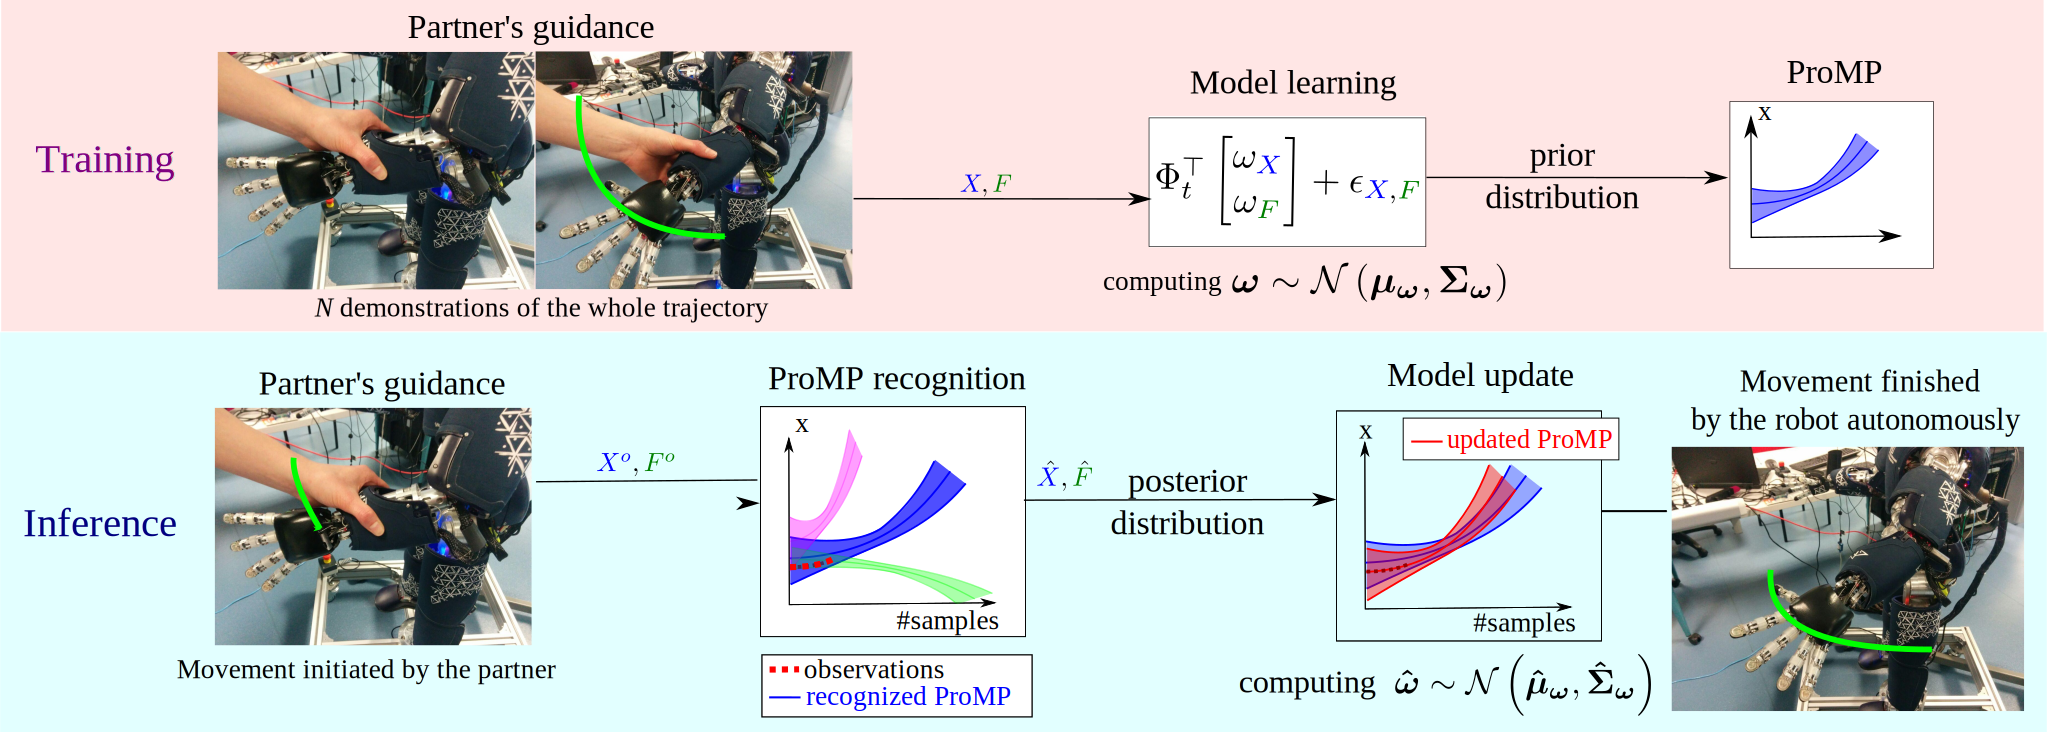
\includegraphics[width=\hsize]{img/conceptualProMPV3.pdf}
\caption{Concepte d'utilisation des ProMPs dans lequel le robot prédit la trajectoire a effectuer dans le cadre de tâche collaborative. En haut : phase d'apprentissage, où les ProMPs sont apprises à partir de plusieurs démonstrations guidés par un humain. Bas : phase d'inférence phase (en line),  où le robot reconnaît, à partir d'un mouvement initié par son partenaire, la ProMP courante et où il prédit l'intention de son partenaire, \textit{i.e.}, l'évolution future de la trajectoire initiée.}
%\todo{Might have to add force information if we have time and results}
\label{fig:conceptProMP}
\end{figure}

Dans ce papier, nous décrivons à la fois la théorie et le logiciel sur lesquels se base la capacité du robot à prédire et effectuer les tâches et mouvements associés de manière autonome.
Le logiciel est actuellement implémenté en Matlab et C++; il est open-source, accessible sur \texttt{github}: %\url{https://github.com/inria-larsen/icubLearningTrajectories/tree/master/CppProgram}
\begin{center}
\url{https://github.com/inria-larsen/icubLearningTrajectories}
\end{center}
De plus, il a été testé à la fois en simulation (à l'aide du simulateur Gazebo contenant une simulation du robot iCub) et sur le robot réel. En simulation, pour que l'utilisateur puisse guider physiquement le robot simulé, nous utilisons un appareil haptique nommé ``Geomagic Touch'', capable de faire ressentir à l'utilisateur une simulation des forces que le robot simulé exerce.\footnote{Dans notre expérience, nous n'utilisons pas cette fonctionalité de retour de forces. Nous utilisons cet appareil afin de diriger manuellement le bras du robot dans le simulateur. Ainsi, nous utilisons cet appareil comme un joystick plus naturellement manipulable.}
%, to simulate the physical guidance of the real robot case. 
; sur le robot réel, l'utilisateur attrape physiquement l'avant bras du robot réel pour le guider.

Nous fournissons aussi un exemple pratique du logiciel, permettant de répondre à des problèmes classiques.
Dans l'exemple, les mesures des trajectoires correspondent à la position cartésienne de l'actuateur ainsi que les forces qui y sont exercées.
%Thanks to the Cartesian position information, the robot can continue movements autonomously, without being guided by the human\footnote{

Notons notamment que ce type de mesures diffère de celles utilisées dans les autres études basées sur les ProMPs~\citep{paraschos2015model}, où il s'agissait des valeurs articulaires. L'utilisation de positions Cartésiennes plutôt que des valeurs articulaires nous permet d'exploiter la redondance du bras robotique afin d'effectuer une certaine tâche dans un espace 3D, ainsi que de permettre au robot de bouger son bras de manière plus naturelle pour effectuer la trajectoire voulue (en effet, lors du déplacement du bras robotique, le partenaire ne bouge que l'avant bras du robot, ce qui limite les possibilités de mouvement du robot).
Du point de vu contrôle du iCub, ce choix implique que le iCub définisse ses couples articulaires afin d'effectuer les mouvements à l'aide d'un contrôleur cartésien~\citep{pattacini2010experimental}, plutôt que d'utiliser un contrôleur articulaire. En ce qui concerne les forces, on se base sur une estimation basée sur une modélisation de la dynamique du robot, et qui utilise les valeurs des capteurs de couple 6D~\citep{ivaldi2011computing,fumagalli2012force}.
Tous les détails des expériences sont présentés dans ce papier et dans le tutoriel du logiciel.
%}.
%\todo{add forces info if we have done it} 
%Thanks to the force information, the robot can detect if the user's forces are larger than the ones it has previously learned: in this case, the robot assumes that the current movement is probably a new demonstration of a new primitive (\textit{e.g.}, a new task, different from the one previously learned) and then instead of trying to guess the goal using the information of the previous primitive, it can follow the users' movement to learn a new movement primitive.

Pour résumer, les contributions de ce papier sont les suivants :
\begin{itemize}
\item  une description de la théorie utilisée dans ce logiciel basée sur la méthode ProMPs et permettant de prédire la trajectoire et le but désirés par l'utilisateur du robot lors d'interaction physique entre le partenaire et le robot. Elle fournie notamment les fonctionnalités suivantes : reconnaissance de la tâche courante, estimation de la durée de la tâche, prédiction de la trajectoire future.;
\item une étude expérimentale concernant comment l'information des forces et moments peuvent améliorer l'estimation de la durée/vitesse de la trajectoire initiée;
\item un software open-source permettant la reconnaissance de l'intention et son application avec le robot iCub, que ce soit en simulation ou avec le robot réel.
\end{itemize}

Ce papier est organisé en plusieurs sections.
Dans la Section~\ref{sec:SOA}, nous résu we review the literature about intentions in Human-Robot Interaction (HRI), probabilistic models for motion primitives and their related software. 
In Section \ref{sec:theory} we describe the theoretical tools that we use to formalize the problem of predicting the intention of the human during interaction. Particularly, we describe the ProMPs and their use for predicting the evolution of a trajectory given early observations. 
In Section \ref{sec:software} we overview the software organization and the interconnection between our software and the iCub's main software, both for the real and simulated robot.
\rev{The following sections are devoted to presenting our software and its use for predicting intention. We choose to present three examples of increasing complexity, with the simulated and real robot.}
We provide and explain in detail a software example for a 1-DOF trajectory in Section \ref{sec:example1DOF}.
In  Sections \ref{sec:3ProMPsAppli} and \ref{sec:appliRealIcub} we present the intention recognition application with the simulated and real iCub, respectively.
\rev{In the first examples with the robot, the ``tasks'' are exemplified by simple reaching movements, to provide simple and clear trajectories that help the reader understand the method, whereas the last experiment with the robot is a collaborative object sorting task.}
Section \ref{sec:video} provides the links to the videos showing how to use the software in simulation and on the iCub.
Finally, in Section~\ref{sec:conclusions} we discuss our approach, its limitations and outline our future developments.

%\newpage
%%%%%%%%%%%%%%%%%%%%%%%%%%%%%%%%%%%%%%%%%%%%%%%%%%%%%%%%%%%%%%%%%%%%%%%%%%%%%%%%
\section{Related Work}\label{sec:SOA}

%\towrite{We will follow the structure that you cited in the introduction if possible. What are the main techniques to solve the problem? Are there papers more focusing on the application? Are there papers more focusing on the theory? Are there different techniques? Here we need to come up to around 20 papers to cite }


In this paper we propose a method to recognize the intention of the human partner collaborating with the robot, formalized as the target and the ''future'' trajectory associated to a skill, modeled by a goal-directed Probabilistic Movement Primitive.   
In this section, we briefly overview the literature about intention recognition in human-robot interaction and motion primitives for  learning of goal-directed robotic skills.

\subsection{Intention during human-robot interaction}
Lors de collaboration homme-robot, la compréhension mutuelle de ces deux agents est primordiale pour assurer la réussite de leur tâche commune.
La compréhension mutuelle signifie que chaque agent est au courant de l'action courante de l'autre, de son statut, de son but, des informations disponibles qu'il peut estimer ou prédire.
La reconnaissance de l'intention n'est qu'une pièce de ce problème, mais joue un rôle cruciale dans l’acquisition de compétence anticipative.

Formaliser l'intention s'avère être une tâche compliquée, notamment parce que fournir une représentation unique qui explique à la fois l'intention moteur (mouvement actuel); l'intention 
 à bas niveau c'est à dire des actions dirigés vers un but (\textit{e.g.} atteindre un objet ciblé et l'attraper); et l'intention à haut niveau, c'est à dires des actions complexes, abstraites, cognitives (\textit{e.g.} changer une ampoule au plafond, en utilisant une échelle, en la grimpant pour afin atteindre l'ampoule, etc.).
Dans \cite{demiris2007prediction}, un récapitulatif est fait sur les différentes approches existantes de la reconnaissance de l'action et de la prédiction de l'intention.

Du point de vue de l'humain, comprendre l'intention du robot signifie qu'il doit déterminer les mouvements ou actions du robot dirigés vers un but, de manière intuitive et non-ambiguë, et qu'il doit comprendre ce que le robot est entrain de faire, ou ce qu'il va faire~\citep{kim2017collaborative}. 
Dans \cite{dragan2014integrating}, on formalise les différence entre~\textit{prédiction} et \textit{lisibilité} : un mouvement est lisible si un observateur peut rapidement inférer son but, tandis qu'un mouvement est prédictible lorsqu'il correspond aux attentes d'un l'observateur connaissant le but. De plus, quand une trajectoire peut être prédite par un observateur à partir d’observation antérieure de celle-ci, on peut dire que la trajectoire n’est pas seulement lisible, mais aussi prédictible.

Les difficultés lors de la génération de mouvements robotiques \textit{lisibles} ont été étudiées dans des études récentes. Par exemple, dans~\cite{dragan2014integrating} on utilise des techniques d'optimisation afin de générer des mouvements à la fois lisible et prédictibles.
Dans~\cite{HuangHAD17}, on applique une méthode d'apprentissage par renforcement inverse à des voitures autonomes afin de sélectionner les mouvements du robot qui contiennent le maximum d'information pour les humains et qui facilite ainsi la compréhension des objectifs du robot.



%"a legible motion is motion that enables an observer to quickly and confidently infer the correct goal G" and predictable  motion  is  motion  that  matches what an observer would expect, given the goal G.", they generate both predictable motion and legible motion using functional gradient descent, but with two different optimization criterion, and they highlight that their legibility model is correct only when the trajectories are contain in a 
%a movement is legible when the robot's goal is clear for the observer whereas a movement is predicable when according to the robot's goal, the motion is predictable.


%\todo{talk about Dragan, Shah, Sciutti with lifting weights, Serena with directional gaze with icub, serena with icub learning objects}

Du point de vue du robot, comprendre l'intention du partenaire humain signifie que le robot doit être capable de déchiffrer l'ensemble des indices verbaux et non-verbaux naturellement générés par le comportement de l'humain afin d'identifier, selon la tâche et le contexte courant, quelle est son intention.
Plus le robot utilise d'informations (\textit{e.g.} signaux mesurables provenant du partenaire humain et de son environnement), plus l'estimation peut être précis.
La forme la plus simple de la reconnaissance de l’intention du partenaire est d'estimer le but d'une action en cours, sous la condition que chaque action correspond à un mouvement dirigé vers un but. \todo{intention}
Dans~\cite{sciutti2013robots}, on montre que les humains attribuent implicitement des intentions dirigées vers un but aux mouvements robotiques, ce qui montre que les humains effectuent un regard d'anticipation vers l'objectif visé. \todo{ ? phrase originel: showed that humans implicitly attribute intentions in form of goals to robot motions, proving that humans exhibit anticipatory gaze towards the intended goal }   
Le regard a aussi été utilisé dans un jeu homme-robot avec le iCub~\cite{Ivaldi2014}, où le robot (respectivement l'humain) suivait le regard de l'humain (respectivement du robot) pour identifier l'objet visé.
Dans~\cite{ferrer2014bayesian}, on propose un algorithme Bayésien permettant de prédire l’intention du mouvement humain, en calculant géométriquement le but le plus probable à partir de la méthode Espérance-Maximisation et d'un simple classificateur Bayésien.
Dans~\citep{wang2012probabilistic}, on propose une méthode appelée modèle dynamique dirigé vers le but (Intention-Driven Dynamics model). Cette méthode est basée sur les Modèles Dynamiques de Processus Gaussiens (GPDM \citep{wang2005gaussian}) et elle permet d'inférer l'intention de l'adversaire humain du robot lors d'un match de ping-pong. Cette intention à estimer correspond à la position ciblée avec la balle, et la méthode se base sur le mouvement entier du partenaire humain, avant même que celui-ci frappe la balle.

\todo{comprendre la phrase : More generally, modeling and descriptive approaches can be used to match predefined labels with measured data \citep{csibra2007obsessed}}.

%\todo{some other examples? }
Une forme plus complexe de reconnaissance de l'intention correspond à l'estimation de la continuation d'une trajectoire à partir des observations antérieures. C'est à dire que l'on veut estimer $[x_{t+1}, \ldots, x_{t+T_{future}}] = f(x_t,x_{t-1},\ldots, x_{t-T_{past}})$. 
\toimprove{Ce problème, similaire à l'estimation des modèles prédictif de la dynamique d'un systeme \todo{c'est bien ça forward dynamics ?}, est fréquemment adressé par les chercheurs en ce qui concerne les modèles de contrôle prédictifs, où être capable de faire évoluer le système dans les temps est la base du controle robotique. }
\sout{This problem, very similar to the estimate of the forward dynamics model of a system, is frequently addressed by researchers in model predictive control, where being able to ``play'' the system evolving in time is the basis for computing appropriate robot controls. }

Quand une trajectoire peut être prédite par un observateur à partir d'observation antérieure de celle-ci, on peut dire que la trajectoire n'est pas seulement \textit{lisible}, mais aussi \textit{prédictible}.
Une approche systématique permettant de prédire une trajectoire est de raisonner en terme de primitives de mouvements, de façon à ce que la séquence de points d'une trajectoire peut être générée par un modèle temporel paramétrique ou par un système dynamique paramétrique.
Par exemple,~\cite{palinko2014communicative} planifie des trajectoires dirigées vers des buts permettant de transporter des objets. Cette méthode de planification permet notamment de connaître les informations sur le poids  des objets transportés.
Plus généralement, dans les approches génératives~\citep{buxton2003learning}, des variables latentes sont utilisées pour modéliser par apprentissage les primitives et ainsi être capable de générer et d'inférer des actions. La section suivante donne plus de détails concernant l'état de l'art des techniques permettant de générer les primitives de mouvements.
%: this is the typical case for movement primitives.

%\todo{some more examples?}
Dans ~\citep{amor2014interaction}, le robot commence par apprendre une primitive d'interaction en regardant deux humains effectuer eux-même la tâche interactive, à l'aide de capture du mouvement. Cette primitive d'Interaction encapsule les dépendances entre deux mouvements humains. Puis, le robot utilise des primitives d'interaction afin d'adapter son comportement aux mouvements de son partenaire. La méthode utilisé est basée sur les Primitives Dynamique de Moteur (Dynamics Motor Primitives~\citep{ijspeert2013dynamical}), où une distribution sur les paramètres des DMP est apprise. Notons que dans notre papier, nous n'utilisons pas la même approche pour apprendre les primitives d'interaction puisque nous modélisons les trajectoires du robot et de l’utilisateur comme une trajectoire unique conjointe, dû au fait que le l'utilisateur et le robot sont en contact physique. De plus, il n'y a pas de latence entre le mouvement initié par le partenaire et celui du robot, puisque le bras du robot est guidé physiquement par le partenaire jusqu'à ce que celui-ci stop le contact.

Beaucoup d'exemples dans la littérature se focalise sur des trajectoires cinématiques, correspondant aux gestes utilisés dans les interactions dyadiques caractérisés par une coordination des actions et des réactions. D'autres s’intéressent à des trajectoires plus complexes, qui correspondent aux trajectoires effectués lors d'interaction physique entre l'homme et le robot, permettant d'effectuer des tâches nécessitant la collaboration des agents et des échanges de forces. En effet, les informations cinématiques fournies par de telles trajectoires ne peuvent pas être analyser sans prendre en compte l’échange haptique et l'estimation des rôles des partenaires (\textit{i.e.}, qui est le leader qui est le follower).

Estimer le rôle actuel du partenaire humain (maître/esclave ou leader/follower) est cruciale puisque l'information des rôle est nécessaire pour adapter correctement la compliance  et l’impédance du robot au niveau des échanges de forces de contact.

Plus important, adapter l'interaction haptique peut permettre au robot d'exprimer qu'il a compris l'intention du partenaire et qu'il est capable de finir la tâche de manière autonome, en imitant le même type de communication non verbale qui est typique chez l'humain.

Par exemple, dans~\citep{gribovskaya2011motion}, le robot infère l'intention de l'humain en utilisant les mesures des forces humaines et en utilisant les modèles de mixture gaussiennes.
Dans~\citep{rozo2013learning}, l'impédance des bras est adapté en utilisant un modèle basé sur les modèles de mixtures de Gaussienne, sur les forces mesurées  et sur les informations visuelles.
Beaucoup d’études se focalisent sur l'abilité du robot à agir seulement quand et selon comment l'utilisateur le souhaite~\citep{carlson2008human}\citep{soh2015learning} , d'autres sur la capacité au robot de ne pas interférer contre les forces de son partenaire~\citep{jarrasse2008can} ou de ses actions~\citep{baraglia2016initiative}.


%\todo{some examples?}

In this paper, we describe our approach to the problem of recognizing the human intention during collaboration by providing an estimate of the future intended trajectory to be performed by the robot. In our experiments, the robot does not adapt its role during the physical interaction, but simply switch from follower to leader when the human breaks contact with it. 

\section{MA VIEILLE PARTIE}

Dans cer papier, on souhaite que notre robot prédise l'intention de son partenaire afin de finaliser un mouvement et une action par lui même. Beaucoup d'autres travaux de recherche necessite cette abilité.


Dans \cite{ferrer2014bayesian}, il s'agit de prédire les mouvements d'un humain en utilisant une méthode appelée Prédiction Bayesienne de l'Intention du Mouvement Humain (BHMIP).
Cette méthode se base sur des calculs géométriques permettant de trouver la destination la plus probable de l'humain ainsi que sur l'algorithme Esperance-Maximisation 
Puis, pour trouver la prédiction la plus performante, ils utilisent un classifieur Bayesien. Cette méthode a l'avantage d'être indépendant du type d'environnement et qu'il ne nécessite pas de calculs intensifs.

D'autres études utilisent la capacité d'inférence pour adapter l'impédance des robots.
Dans \citep{gribovskaya2011motion}, le robot infère l'intention de l'humain grâce a la mesure des forces de celui ci et en utilisant des modèles de mixtures de gaussiennes. Dans \citep{wang2009hmm}, ils utilisent des Hidden Markov Models pour apprendre comment compenser des forces physique potentielles. Leur robot utilise cette méthode afin de serrer la main de son partenaire, en mesurant l'impédance de ce dernier et en reconnaissant quel type de mouvement il doit suivre. Dans~\citep{rozo2013learning}, un bras robotique mesure les forces et les informations visuelles afin d'adapter son impédance, en utilisant ici aussi des modèles de mixtures gaussiennes.
Dans notre étude, le robot utilise l'information des forces et des moments afin d'estimer l’intention de son partenaire ainsi que de détecter la vitesse du mouvement.

Dans une autre thématique de recherche, les robots utilisent la capacité de prédiction de l'intention humaine afin d'adapter leur comportement (maître/esclave). En effet, pour collaborer efficacement avec les humains, les robots doivent être rigide quand ils effectuent eux même la tache (maître), tout en restant alerte à la volonté de leur partenaire (c'est à dire qu'il doit rester suffisamment compliant pour permettre à l'utilisateur de contrôler l'action). C'est pourquoi beaucoup d'études se focalisent sur l’habilité du robot à agir uniquement quand et comment son utilisateur le souhaite~\citep{carlson2008human}\citep{soh2015learning} et sur sa capacité à ne pas interférer avec les forces de son partenaire~\citep{jarrasse2008can} ou ses actions~\citep{baraglia2016initiative}.
Dans notre étude, le robot est "esclave" lorsqu'il est guidé par son partenaire (au début du mouvement), puis devient maître lorsqu'il finit le mouvement par lui même.


%To acquire this inference ability, different scenarios have been used.

Dans certaines études, le robot observe d'abord le mouvement du partenaire dans sa totalité avant d'agir.Dans \citep{wang2012probabilistic}, une méthode appelé Intention-Driven Dynamics model permet d'inférer l'intention du partenaire du robot durant un match de ping pong. Cette méthode est une amélioration des Gaussian Process Dynamical Models (GPDM \citep{wang2005gaussian}) et permet au robot d'inférer où la balle va être envoyé, avant même que le partenaire humain ait frappé la balle, grâce à l'analyse du mouvement de celui-ci.

Pour obtenir cette aptitude d'inférence, différentes méthodes existent.
Dans\citep{demiris2007prediction}, un récapitulatif est fait sur les différentes approches concernant la reconnaissance de l'action et de la prédiction de l’intention. La premiers possibilité consiste à faire coïncider les informations mesurées avec des modèles. Pour cela, une première possibilité consiste à utiliser des approches descriptives, où l'on fait correspondre à des labels prédéfinis, les données récoltées. On peut trouver un récapitulatif de ces méthodes descriptives dans~\citep{csibra2007obsessed}. Une deuxième possibilité consiste à utiliser des approches génératives, où l'on utilise des variables latentes afin d'apprendre les informations utiles à l’inférence de l'action. Ce type d'approche se base sur l'utilisation de distribution probabilistes. Un récapitulatif de ces approches génératives peut être trouvé dans~\citep{buxton2003learning}.



Dans \todo{citer Yannis Demiris Prediction of intent in robotics and multi agent systems 2007}, les différentes approches permettant la reconnaissance de l'action et la prédiction de l'intentionnalité sont définis et expliqués. Dans ce document, une architecture générative est mise en évidence, appelé HAMMER (Hierarchical Attentive Multiple Models for Excecution and Recognition). Cette architecture utilise un modele inverse de prédiction \todo{inverse-forward model} afin d'executer une action ou de reconnaitre une action faite par un demonstrateur.

Un probleme sous jacent à la reconnaissance de mouvement est que le robot doit estimer la durée de la trajectoire afin de l'aligner avec les trajectoires qu'il a apprit. Dans notre cas, au début de l'interaction physique entre l'homme et le robot, ce dernier observe un mouvement partiellement guidé par son utilisateur. À partir de ce mouvement partiel, le robot doit d'abord estimer l'etat courant du mouvement afin de comprendre l'intention de son partenaire. Ainsi, il a besoin d'estimer la vitesse du mouvement.

Mathématiquement, la loi de Fitt modélise la durée d'um mouvement. Une assumption de ce modèle est que la durée du mouvement est fonction linéaire de la difficulté à atteindre la cible\cite{fitts1992information}. Dans~\cite{langolf1976investigation}, ils montrent qu'en modifiant la taille de la cible, la forme du mouvement change. Ainsi, il est difficile d'appliquer la théorie de la loi de Fitt quand la taille de la cible peut varier. Dans~\cite{langolf1976investigation} et \cite{soechting1984effect}, ils confirment cette idée en montrant que la même forme du mouvement change avec la précision necessaire pour atteindre la position but du mouvement.

Une autre méthode, souvent utilisé en informatique est appelée Dynamics Time Warping\footnote{Déformation temporelle dynamique} (DTW). 
Cette méthode permet de trouver la corrélation entre deux trajectoires dont la durée diffère, de maniere plus robuste qu'en utilisant la distance euclidienne. Dans \cite{amor2014interaction}, cet algorithme est modifié afin de permettre de faire coïncider des mouvements partiels avec une trajectoire référence.
Beaucoup d'améliorations et de variations de cette méthode existe. Dans~\cite{keogh2002exact}, 
ils proposent des méthodes permettant d'améliorer l'indexation, et ainsi d’accélérer la vitesse de calcul de l'algorithme. On trouve ainsi les méthodes FastDTW, Lucky Time Wraping ou encore FTW.  Dans\cite{silva2016speeding}, ils commencent par expliquer et comparer ces méthodes, puis ils ajoutent leur propre méthode appelé Pruned Warping Path, qui accélère encore plus la vitesse calculatoire. De plus, cette méthode permet de supprimer les données improbables. Mais le principale désavantage de toutes ces méthodes basés sur DTW est qu'elles ne préservent pas la forme globale de la trajectoire (la trajectoire est déformée).

Dans \cite{maeda2014learning}, des primitives de mouvements sont apprises à l'aide d'apprentissage probabiliste. Ils améliorer l'estimation des mouvements en utilisant une méthode différente. Celle-ci utilise aussi une modélisation à base de gaussiennes de la fonction de déformation du temps, et au lieu d'utiliser la méthode DTW, cette méthode force l'alignement locale entre les deux mouvements, sans "sauter" des indexes. Ainsi, les trajectoires obtenues sont plus réalistes, plus régulière, et cette méthode préserve la forme globale des trajectoires.

\subsection{\quest{Movement primitives /} Primitives de mouvement}


%\todo{@Alex: please revise this entire section about movement primitives}

%Movement primitives can be encoded into a set of parameters in dynamical system as well as in stochastic models. Dynamical systems define the dynamic of movements as a vector field, where each motion pattern is expressed by a closed curve in this field. This field attracts the robot's movement to the reference one, and this attraction assures the stabilization of the robot's movement. Many methods exist for that purpose.
%Dynamic Motor Primitives (DMP) is one of these methods, presented in \cite{schaal2006dynamic}, that formalized mathematically movement primitives as stable non-linear attractor systems. This method consists of adding a term to a stable dynamical model. This term makes the system follow specific trajectories. This methods has been used in several studies with robotic manipulators, in particular for reaching motions. It has been improved in \cite{ijspeert2013dynamical}.

\quest{Movement Primitives (MPs) is a well established paradigm for representing complex motor skills.}

Les modèles utilisant des primitives de mouvement \toimprove{(MPs)} sont une référence quand il s'agit de représenter des capacités motrices complexes.

%MPs can be encoded into a set of parameters in dynamical system as well as in stochastic models. Dynamical systems define the dynamic of movements as a vector field, where each motion pattern is expressed by a closed curve in this field. This field attracts the robot's movement to the reference one, and this attraction assures the stabilization of the robot's movement. Many methods exist for that purpose.
\rev{The most known method for representing movement primitives is probably the} Dynamic Movement Primitives (DMPs)~\cite{ijspeert2013dynamical,schaal2006dynamic,meier2016probabilistic}. \rev{DMPs} use a stable non-linear attractor in combination with a forcing term to represent the movement. The forcing term enables to follow specific movement, while the attractor asserts asymptotic stability. 
\rev{In a recent paper, \cite{meier2016probabilistic} proposed an extension to DMPs, called PDMP (Probabilistic Dynamic Movement Primitive). This method improves DMP with probabilistic properties to measure the likelihood that the movement primitive is executed correctly and to perform inference on sensor measurement. However, The PDMPs do not have a data-driven generalization and can deviate arbitrarily from the demonstrations. This last difference can be critical for our applications with the humanoid robot iCub, since uncertainties are unavoidable and disturbances may happen frequently and de-stabilize the robot movement (for example, an unexpected collision during the movement). Thus, the ProMPs method is more accurate for our software.}



\rev{\cite{ewerton2015learning}, \cite{paraschos2013probabilisticTrajectory} and \cite{maeda2014learning} 
%\todo{I don't find this paper on the internet, so I cannot cite it. Can you give me the bibtex?} 
compared ProMPs and DMPs for learning primitives and specifically interaction primitives. With the DMP model, at the end of the movement, only a dynamic attractor is activated. Thus, it always reach a stable goal. 
The properties allowed by both methods are temporal scaling of the movement, learning from a single demonstration, and generalizing to new final position. 
With ProMPs, we have in addition the ability to do inference (thanks to the distribution), to force the robot to pass by several initial via-points (the early observations), to know the correlation between the input of the model, and to co-activate some ProMPs. 
In our study, we need these features, because the robot must determine a trajectory that passes by the early observations (beginning of the movement where the user guides physically the robot). 
}
%Moreover, in an experiment of our paper, we assume the robot uses only a sub-part of the inputs of the model to do the inference (e.g. only Cartesian position is used). By using ProMPs instead of DMP, the program is able to compute the expectation of the other inputs (forces), from the correlation between the inputs).\\
%}

%The DMPs have been extensively used for controlling robotic manipulators for reaching movements.
%An probabilistic approach to DMPs improvement of this method, called Probabilistic Dynamic Movement Primitive (PDMP), is presented in \cite{meier2016probabilistic}. %This method shares the advantages of DMPs, and on,% a failure detection feature thanks to a probabilistic learning. In \cite{denivsa2016learning}, they use a method called Compliant Movement Primitive (CMP) based on Torques Primitives (TP) and Dynamic Movement Primitives (DMP). First, the trajectory of the movement is shown and encoded in DMP. Then, a robot executes the movement by using a feedback control. The executed trajectories are then encoded as radial basis functions in a TP. This TP is used as a feed-forward term. By using this method, robots can learn the specificities of the dynamical model of each task, instead of mathematical models that cannot take into account all these specificities. In \cite{mulling2013learning}, they use DMPs to allow a robot to learn a set of elementary table tennis hitting movements, thanks to kinesthetic learning. Then, they use a mixture of motor primitives (MoMP) to generalize the learned movements to a wider range of situations.
A Recurrent Neural Networks (RNN) approach \cite{billard2001learning} used a 
hierarchy of neural networks to simulate the activation of areas in human brain. The network can be trained to infer the state of the robot at the next point in time, given the current state. The authors propose to train the RNN by minimizing the error between the inferred position of the next time step and the ground-truth obtained from demonstrations.

%%A short explanation is done here \url{https://studywolf.wordpress.com/2013/11/16/dynamic-movement-primitives-part-1-the-basics/}.
%An improvement of this method, called Probabilistic Dynamic Movement Primitive (PDMP), is presented in \cite{meier2016probabilistic}. This method has the same advantages as DMP with, in addition,% a failure detection feature thanks to a probabilistic learning. In \cite{denivsa2016learning}, they use a method called Compliant Movement Primitive (CMP) based on Torques Primitives (TP) and Dynamic Movement Primitives (DMP). First, the trajectory of the movement is shown and encoded in DMP. Then, a robot executes the movement by using a feedback control. The executed trajectories are then encoded as radial basis functions in a TP. This TP is used as a feed-forward term. By using this method, robots can learn the specificities of the dynamical model of each task, instead of mathematical models that cannot take into account all these specificities. In \cite{mulling2013learning}, they use DMPs to allow a robot to learn a set of elementary table tennis hitting movements, thanks to kinesthetic learning. Then, they use a mixture of motor primitives (MoMP) to generalize the learned movements to a wider range of situations.
%All these dynamical methods allow to recognize and predict movements.
%allow to infer following input (\textit{e.g.} for a movement the position of the next iteration) and to improve the inference ability by optimizing the error between inferred positions and their real values (measured by the robot). In \cite{billard2001learning}, they use a 
%

%
%Another dynamical method is Recurrent Neural Networks (RNN). The idea of such Neural Networks is to infer the following input (\textit{e.g.} for a movement the position of the next iteration) and to improve the inference ability by optimizing the error between inferred positions and their real values (measured by the robot). In \cite{billard2001learning}, they use a hierarchy of artificial neural network models based on some human's brain areas. This model allows to reproduce all their tested human's arm motions efficiently.

Hidden Markov Models (HMMs) for  movement skills were introduced by~\cite{fine1998hierarchical}.
This method is often used to categorize movements, where a category represents a movement primitive. This method also allows to represent the temporal sequence of a movement. 
In \cite{nguyen2005learning} they use learned Hierarchical Hidden Markov Model (HHMMs) to recognize human behaviors efficiently. 
In \cite{ren2002human} they present the Primitive based Coupled-HMM (CHMM) approach, for human natural complex action recognition. In this approach, each primitive is represented by a Gaussian Mixture Model.


Adapting Gaussian Mixture Models is another method used to learn physical interaction with %distribution \todo{why did you wrote "distributions"?} 
learning. In \cite{evrard2009teaching} they use GMMs and Gaussian Mixture Regression to learn, in addition to the position (joint information), force information. Using this method, a humanoid robot is able to collaborate in one dimension with its partner for a lifting task. In our paper, we will also use (Cartesian) position and force information to allow our robot to interact physically with its partner.

%With regard to stochastic models, a well known method is the Hidden Markov Models (HMMs). This method is often used to categorize movements, where a category represents a movement primitive. This method also allows to represent the temporal sequence of a movement. Improvements of this model exist to encode complex spatio-temporal features.  For example, Hierarchical HMMs (HHMMs) have been introduced in \cite{fine1998hierarchical} to include a hierarchy of hidden states. In \cite{nguyen2005learning}, they use learned HHMMs to recognize human behaviours efficiently. They compare their method with other HHMMs methods and show that thanks to their learning, the results are more efficient. In \cite{ren2002human} they present an approach called Primitive based Coupled-HMM (CHMM), for human natural complex action recognition. In this approach, each primitive is represented by a Gaussian Mixture Model.


A sub-problem of movement recognition is that robots need to estimate the duration of the trajectory to align a current trajectory with learned movements. In our case, at the beginning of the physical Human-Robot Interaction (pHRI), the robot observes a partial movement guided by its user. Given this partial movement, the robot must first estimate what the current state of the movement is to understand what its partner intent is. Thus, it needs to estimate the partial movement's speed.

Fitts' law models the movement duration for goal-directed movements. This model is based on the assumption that the movement duration is a linear function of the difficulty to achieve a target\cite{fitts1992information}. In \cite{langolf1976investigation}, they show that by modifying the target's width, the shape of the movement changes. Thus, it is difficult to apply Fitt's law when the size of the target can change. In \cite{langolf1976investigation} and \cite{soechting1984effect}, they confirm this idea by showing that the shape of the movement changes with the accuracy required by the goal position of the movement. 

 Dynamics Time Warping (DTW) is a method to find the correlation between two trajectories that have different durations, in a more robust way than the Euclidean distance. In \cite{amor2014interaction}, they modify the DTW algorithm to match a partial movement with a reference movement.
Many improvements over this method exist. In~\cite{keogh2002exact}, they propose a robust method to improve the indexation. The calculation speed of DTW is improved using different methods, such as FastDTW, Lucky Time Warping or FTW. An explanation and comparison of these methods is presented in \cite{silva2016speeding}, where they add their own computation speed improvement by using a method called Pruned Warping Paths. This method allows the deletion of unlikely data. However, a drawback of this well-known DTW method is they don't preserve the global trajectory's shape. 

In \cite{maeda2014learning}, where they use a probabilistic learning of movement primitives, they improve the duration estimation of movements by using a different time warping method. This method is based on a Gaussian basis model to represent a time warping function and, instead of DTW, it forces a local alignment between the two movements without ``jumping'' some index. Thus, the resulting trajectories are more realistic, smoother, and this method preserves the global trajectories' shapes.


\medskip

For inferring the intention of the robot's partner, we use Probabilistic Movement Primitives (ProMPs), \cite{paraschos2013probabilistic}). Specifically, we use the ProMP's conditioning operator to adapt the learned skills according  to observations. The ProMPs can encode the correlations between forces and positions and allow better prediction of the partner's intention.
Further, the phase of the partner's movement can be inferred  and therefore  the robot can adapt to the partner's velocity changes. ProMPs are more efficient for collaborative tasks, as shown in~\cite{maeda2014learning}, where in comparison to DMPs, the root-mean square error of the predictions is lower.


%In our case, we use the Probabilistic Movement Primitives method (ProMP,\cite{paraschos2013probabilistic}) that has the advantage to exhibit all the following properties: conditioning the trajectory to pass by via-points (this property is used here to adapt the robot's movement according to its partner's will); using correlation between different information (used here to correlate forces and positions); inferring and following the phase of the partner's movement (thanks to this property, the robot recognizes a movement even if the partner's velocity changes). 
%This method is close to DMP, but ProMPs are more efficient for our goal. Indeed, in~\cite{maeda2014learning} we see that when we use DMP, the root-mean square prediction error of a collaborative movement is bigger than when we use ProMPs. Also, in \cite{paraschos2013probabilisticTrajectory}, we see that when we modify the end of the trajectory, the movement is inside of the learned movement distribution, whereas with DMPs, the new movement is out of the learned distribution. 
%This could be critical in our case since our robot learns the CoM trajectory used to maintain its balance during the whole movement.\\
%amélioration temps modulation marco
%\cite{paraschos2015model} 
%permet d'apprendre en plus de la trajectoire à suivre, les actions que le robot doit effectuer (eg il apprend le controle qu'il doit effectuer au court de cette trajectoire, controle dont la raideur est variable grace a la distribution apprise.
%\subsection{Probabilistic models for prediction}

%\todo{Already placed in the previous paragraphs}


\subsection{Related open-source software}

One of the goals of this paper is to introduce an open-source software for the iCub (but potentially for any other robot), where the ProMP method is used to recognize human intention during collaboration, so that the robot can execute initiated actions autonomously.
%continue trajectories guided by a human user.
This is not the first open-source implementation for representing movement primitives: however, it has a novel application and a rationale  
%\todo{what does this mean ?} 
that makes it easy to use with the iCub robot.

%We can find other open-source softwares that implement other methods applied on other robots. In the following table, we give a partial list of some of these softwares.

In Table 1
%\ref{table:software}, 
we report on the main software libraries that one can use to learn movement primitives. Some have been also used to realize learning applications with iCub, \textit{e.g.}, \cite{lober2014multiple,2013ACTI2891} or to recognize human intention.
However, the software we propose here is different: it provides an implementation of ProMPs used explicitly for intention recognition and prediction of intended trajectories. It is interfaced with iCub, both real and simulated, and addresses in the specific case of physical interaction between the human and the robot. 
In short, it is a first step towards adding intention recognition ability to the iCub robot.%This skill is used to allow the robot to finish a movement on its own, where each movement can be linked to a specific action.


\begin{table}
\begin{center}
\begin{tabular}{|p{5.5cm}|p{3cm}|p{2cm}|p{1.5cm}|p{2cm}| p{2cm}|}
  \hline
  \textbf{Software/library} & \textbf{Method} & \textbf{Code link} & \textbf{Language} & \textbf{Robot} & \textbf{Reference(s)}\tabularnewline
  \hline
Dynamical System Modulation for Robot Adaptive Learning via Kinesthetic Demonstrations & GMR & \cite{gmr} & Matlab & Hoap3 & \cite{hersch2008dynamical}\tabularnewline
  \hline
pbdlib-matlab & HMM, GMM, and others & \cite{pbdlib} & Matlab & Baxter & \cite{Calinon16JIST} \tabularnewline
  \hline
% Intention\_Recognition \_Human\_Robot\_Interaction & SURF matching & \cite{HumanIntention} & C++, python and others &  SeekurJr with manipulator & \\
%  \hline
DMP learning with GMR  & DMP and GMR & \cite{StatisticalDynamical}  & Matlab or C & Coman & \cite{Calinon12Hum} \tabularnewline
\hline
Stochastic Machine Learning Toolbox & Kernel Functions, Gaussian Processes, Bayesian Optimization & \cite{smlt} & C++ or Python &  | & \tabularnewline
\hline
  pydmps & DMP & \cite{pydmps} & Python & Sarcos & \cite{ijspeert2013dynamical}\tabularnewline
  \hline
   Dynamical Systems approach to Learn Robot Motions & GMM, SEDS & \cite{seds} & Matlab & iCub & \cite{khansari2011learning}, \cite{khansari2012dynamical} \tabularnewline
  \hline

Function Approximation, DMP, and Black-Box Optimization (dmpbbo) &  DMP  & \cite{dmpbbo} & Python or C++ & iCub & \cite{lober2014multiple,2013ACTI2891} \tabularnewline
  \hline  
  Learning Motor Skills from Partially Observed Movements Executed at Different Speeds & ProMP & \cite{marcoProg} & Matlab or Python & | & \cite{ewerton2015learning}\tabularnewline
  \hline
\rowcolor{yellow} icubLearningTrajectories & ProMP & \cite{icubLearningTrajectories} & Matlab and C++ & iCub & | \tabularnewline
\hline
\end{tabular}
\end{center}

\label{table:software}
\caption{Open-source software libraries implementing Movement Primitives and their application to different known robots.}
\end{table}



%\newpage
%%%%%%%%%%%%%%%%%%%%%%%%%%%%%%%%%%%%%%%%%%%%%%%%%%%%%%%%%%%%%%%%%%%%%%%%%%%%%%%%
\section{Theoretical framework}
\label{sec:theory}

%This section is devoted to explain the theoretical framework and the methods implemented in the first module of our software, that implements ProMPs. 
\quest{In this section we present the theoretical framework that we use to tackle the problem of intent recognition: we describe the ProMPs and how they can be used to predict trajectories from early observations.}

Dans cette section nous présentons le cadre théorique que nous utilisons pour nous attaquer au problème de la reconnaissance d'intention. C'est-à-dire que nous allons détailler le fonctionnement des méthodes ProMPs et comment elles peuvent être utilisées pour prédire des trajectoires à partir des observations initiales.

%is devoted to explain the theoretical framework and the methods implemented in the first module of our software, that implements ProMPs. 
\quest{In Section~\ref{LearningSimpleProMP} we formulate the problem of learning a primitive for a simple case, where the robot learns the distribution from several demonstrated trajectories. 
In Section~\ref{sec:predict} we formulate and provide the solution to the problem of predicting the ``future'' trajectory from early observations (\textit{i.e.}, the initial data points).
In Section~\ref{sec:predictDuration} we discuss the problem of predicting the time modulation, \textit{i.e.}, predicting the global duration of the predicted trajectory. This problem is non-trivial, as by construction the demonstrated trajectories are ``normalized'' in duration when the ProMP is learned. \footnote{In some tasks, \textit{e.g.}, reaching, it is reasonable to assume that the difference of duration of the demonstrated trajectories is negligible; however, in other tasks the duration of the demonstrated trajectories may vary significantly.}
In Section \ref{sec:ManyProMP} we explain how to recognize, from the early observations, to which of many known skills (modeled by ProMPs) the current trajectory belongs.
In all these sections we tried to present the theoretical aspects related to the use of ProMPs for the intention recognition application.
}
\quest{Practical examples of these theoretical problems are presented and explained later in sections \ref{sec:example1DOF} - \ref{sec:appliRealIcub}. 
Section \ref{sec:example1DOF} explains how to use our software, introduced in Section \ref{sec:softwareOverview}, for learning one ProMP for a simple set of 1-DOF trajectories.
Section \ref{sec:3ProMPsAppli} presents an example with the simulated iCub in Gazebo, while Section \ref{sec:appliRealIcub} presents an example with the real iCub.
}


Dans la Section~\ref{LearningSimpleProMP} nous formulons le problème d'apprentissage de primitives à l'aide de la méthode ProMP pour un cas simple. Dans ce cas, le robot apprend la distribution à partir de plusieurs trajectoires de démonstration. Dans la Section~\ref{sec:predict} nous formulons et fournissons la solution au problème de prédiction de la trajectoire \og future \fg{} à partir des premières observations sur la trajectoire.
Dans la Section~\ref{sec:predictDuration} nous discutons du problème de prédiction de la \toimprove{modulation du temps}, c'est-à-dire la prédiction de la durée globale de la trajectoire prédite. Ce problème n'est pas trivial parce que les trajectoires de démonstration sont \og normalisées \fg{} par rapport au temps pendant l'apprentissage des primitives avec la méthode ProMP. \toimprove{Pour certaines taches, comme des taches d'atteignabilité par exemple, il est raisonnable de supposer que la différence de durée des trajectoires est négligeable ; cependant d'autres taches \toimprove{exigent davantage de précision et} la durée des trajectoires de démonstration peut significativement varier.}
Dans la Section~\ref{sec:ManyProMP} nous expliquons comment reconnaitre, à partir des premières observations, laquelle des nombreuses compétences apprises (modélisées par des méthodes ProMP) doit être sollicitée.
Ainsi dans ces trois sections nous présentons les aspects théoriques liés à l'utilisation de méthodes ProMP dans le but de reconnaitre des intentions.

Nous illustrons ces problèmes théoriques dans les Sections~\ref{sec:example1DOF} à \ref{sec:appliRealIcub}. Dans la Section~\ref{sec:3ProMPsAppli} nous détaillons un exemple avec un robot iCub simulé avec \toimprove{Gazebo\ref{.}} et dans la Section~\ref{sec:appliRealIcub} nous présentons un exemple cette fois-ci avec le robot iCub réel.

%Before presenting the examples, 

\subsection{Notation}\label{sec:notation}
%To ease the reading and the understanding of the theoretical tools, we will use the following notations:

\quest{To facilitate understanding of the theoretical framework, we first introduce the notations we use in this section and throughout the remainder of the paper.}

Pour faciliter la compréhension du cadre théorique nous introduisons tout d'abord les notations que nous utilisons tout au long de cette thèse.

\noindent
\textbf{Trajectories:}
\begin{itemize}
\item $X(t)\in \mathbb{R}^3, X(t) = [x(t), y(t), z(t)]^\top$: the x/y/z-axis Cartesian coordinate of the robot's end-effector.
\item $F(t) \in \mathbb{R}^6, F(t) = [f_x, f_y, f_z, m_x, m_y, m_z]^\top$: the wrench contact forces, \textit{i.e.} the external forces and moments measured by the robot at the contact level (end-effector).
\item $\xi(t) \in \mathbb{R}^D$: the generic vector containing the current value or state of the trajectories at time $t$. It can be mono-dimensional (\textit{e.g.} $\xi(t) = [z(t)]$), or multi-dimensional (\textit{e.g.} $\xi(t) = [X(t), F(t)]^\top$), depending on the type of trajectories that we want to represent with the ProMP.


\item $\Xi = \Xi_{[1:t_{f}]} = [\xi(1), \ldots, \xi(t_{f})]^\top \in \mathbb{R}^{D \cdot t_{f}}$ is an entire trajectory, consisting of $t_f$ samples or data points. 

\item $\Xi_{i[1:t_{fi}]}$ is the $i$-th demonstration (trajectory) of a task, consisting of $t_{fi}$ samples or data points. 

%For example, $\Xi_{i[1:t_{fi}]}= [\xi_i(1), \ldots, \xi_i(t_{fi})]^\top $ is the $i$-th trajectory.

%\item $t_{fi}$: total number of samples of a $\Xi_i$ trajectory;
%\item $\Xi = \Xi_{[1:t_{f}]} \in \mathbb{R}^{D \cdot t_{f}}$: a trajectory. For example, $\Xi_{i[1:t_{fi}]}= [\xi_i(1), \ldots, \xi_i(t_{fi})]^\top $ is the $i$-th trajectory.
\end{itemize}
\textbf{Movement Primitives:}
\begin{itemize}
\item $k \in [1:K]$: the $k$-th ProMP, among a set of $K$ ProMPs that represent different tasks/actions. 
\item $n_k$: number of recorded trajectories for each ProMP.
\item $S_k = \{\Xi_{\{k,1\}},\ldots,\Xi_{\{k,n_k\}}\}$: set of $n_k$ trajectories for the $k$-th ProMP. 
%For clarity, we consider $\Xi_i \equiv \Xi_{\{k,j\}}$.
\end{itemize}
\begin{itemize}
\item $\xi(t) = \Phi_t \boldsymbol{\omega} + \epsilon_\xi$ is the model of the trajectory with:
\begin{itemize}
\item $\epsilon_\xi \sim \mathcal{N}(0, \beta)$: expected trajectory noise.
\item $\Phi_t \in \mathbb{R}^{D\times D \cdot M}$: radial basis functions (RBFs) used to model trajectories. It is a block diagonal matrix.
\begin{itemize}
\item[-] $M$: number of RBFs.
\item[-] $ \psi_{ji}(t) =\dfrac{e^{-(t - c_i)^2 \over 2h}}{\sum_{m=1}^{M} e^{-(t - c_m)^2 \over 2h} }$: $i$-th RBF for all inputs $j \in [1:D]$. 

It must be noted that the upper term comes from a Gaussian $\frac{1}{\sqrt{2\pi h}} e^{-(t - c_i)^2 \over 2h}$, where $ c_i, h$ are respectively the center and variance of the $i$-th Gaussian. In our RBF formulation, we normalize all the Gaussians.
ˆ%\item[-] $ c_i, h$: center and variance parameters of the $i$-th Gaussian.
\end{itemize}
\item $\boldsymbol{\omega} \in \mathbb{R}^{D \cdot M}$: time-independent parameter vector weighting the RBFs, \textit{i.e.}, the parameters to be learned.

\end{itemize}

\item $p(\boldsymbol{\omega}) \sim \mathcal{N}(\mu_{\boldsymbol{\omega}}, \Sigma_{\boldsymbol{\omega}})$: normal distribution computed from a set $\{\boldsymbol{\omega}_1, \ldots, \boldsymbol{\omega}_n\}$. It represents the distribution of the modeled trajectories, also called \textit{prior} distribution.
%\footnote{It must be noted that in the original ProMP paper \cite{paraschos2013probabilistic} the prior distribution $p(\boldsymbol{\omega})$ is written as $p(\boldsymbol{\omega}) =\theta \sim \mathcal{N}(\mu_\omega, \sigma_\omega)$. However, in robot learning $\theta$ is often used as a variable for parameters to be learned. To avoid ambiguities, we decide to employ simply $p(\boldsymbol{\omega})$. \todo{Controler} \rev{I am not sure that what you wrote is correct. May be better to write: the distribution is called $p(\omega; \theta)=\mathcal(\omega |\mu_\omega, \Sigma_\omega )$ over the weight vector $\omega$, with parameters $\theta$}}



\end{itemize}
\textbf{Time modulation:}
\begin{itemize}
\item $\bar{s}$: number of samples used as reference to rescale all the trajectories to the same duration.
\item $\Phi_{\alpha_i t} \in \mathbb{R}^{D\times D \cdot M}:$ the RBFs rescaled to match the $\Xi_i$ trajectory duration.
\item $\alpha_i = { \bar{s} \over t_{fi}}$: temporal modulation parameter of the $i$-th trajectory .
\item $\alpha = \Psi_{\delta_{n_o}}\boldsymbol{\omega}_\alpha + \epsilon_\alpha$ is the model of the function mapping $\delta_{n_o}$ into the temporal modulation parameter $\alpha$, with:

\begin{itemize}
\item[-] $\Psi$: a set of RBFs used to model the mapping between $\delta_{n_o}$ and $\alpha$;
\item[-] $\delta_{n_o}$ is the variation of the trajectory during the first $n_o$ observations (data points); it can be $\delta_{n_o}=\xi(n_o) - \xi(1)$ if the entire trajectory variables (\textit{e.g.}, Cartesian position, forces, etc.) are considered, or more simply $\delta_{n_o}= X(n_o) - X(1)$ if only the variation in terms of Cartesian position is considered;
%\item $ \theta_\alpha \sim \mathcal{N}(\mu_{\boldsymbol{\omega}_\alpha}, \sigma_{\boldsymbol{\omega}_\alpha})$: normal distribution of the $\{\boldsymbol{\omega}_{\alpha_1},\ldots, \boldsymbol{\omega}_{\alpha_n} \}$ dataset.
\item[-] $\boldsymbol{\omega}_\alpha$: the parameter vector weighting the RBFs of the $\Psi$ matrix. 
%It provides an overall fit for all the $\alpha_i$.

\end{itemize}
\end{itemize}
\textbf{Inference:}
\begin{itemize}
%\item $n_o = t_{no}$: number of early observations used for the prediction.
\item $\Xi^o =[X^o, F^o]^\top = [\xi^o(1),\ldots, \xi^o(n_o)]^\top$: early-trajectory observations, composed of $n_o$ data points.
\item $\Sigma_\xi^o$: noise of the initiated trajectory observation.
\item $\hat{\alpha}$: estimated time modulation parameter of a trajectory to infer.
\item $\hat{t}_f ={\bar{s} \over \hat{\alpha}}$: estimated duration of a trajectory to infer.
\item $\Xi^* = [\xi^o(1),\ldots, \xi^o(n_o), \xi^*(n_o+1),\ldots, \xi^*(t_f)]$: ground truth of the trajectory for the robot to infer.
\item $\hat{\Xi} =[\hat{X}, \hat{F}]^\top = [\xi^o(1),\ldots, \xi^o(n_o), \hat{\xi}(n_o + 1),\ldots,\hat{\xi}(\hat{t}_f)]^\top$: the estimated trajectory.
\item $p(\hat{\boldsymbol{\omega}}) \sim \mathcal{N}(\hat{\mu}_{\boldsymbol{\omega}}, \hat{\sigma}_{\boldsymbol{\omega}})$: posterior distribution of the parameter vector of a ProMP using the observation $\Xi^o$.
%\item $\hat{\theta}_\alpha \sim \mathcal{N}(\hat{\mu}_{\boldsymbol{\omega}_\alpha}, \hat{\sigma}_{\boldsymbol{\omega}_\alpha})$: posterior distribution of the parameter vector of the parameter $\alpha$ using the observation.
%\item $ \hat{\boldsymbol{\omega}} \overset{\mathrm{def}}{=}  \hat{\boldsymbol{\mu}_\omega}$ \todo{is it correct to write it like that?}: parameter vector used to select a trajectory in the posterior distribution $\hat{\theta}$.
%\item $ \hat{\boldsymbol{\omega}_\alpha} = \hat{\mu_{\boldsymbol{\omega}_\alpha}}$: new mean of the distribution of the parameters vector of a modelled $\alpha$ phase, after inference.


\item $\hat{k}$: index of the recognized ProMP from the set of $K$ known (previously learned) ProMPs.
\end{itemize}


\noindent
\textbf{Trajectoires :}
\begin{itemize}
	\item $X(t)\in \mathbb{R}^3, X(t) = [x(t), y(t), z(t)]^\top$ : l'axe x/y/z pour représenter les coordonnées cartésiennes de l'effecteur du robot.
	\item $F(t) \in \mathbb{R}^6, F(t) = [f_x, f_y, f_z, m_x, m_y, m_z]^\top$ : la \toimprove{wrench} des forces de contact, c'est-à-dire les forces externes et les moments mesurées par le robot au \toimprove{niveau du contact (effecteur).}
	\item $\xi(t) \in \mathbb{R}^D$ : le vecteur générique contenant la valeur courante ou l'état des trajectoires au temps $t$. 
	Il peut être mono-dimensionnel (\textit{e.g.}, $\xi(t) = [z(t)]$), ou multidimensionnel(\textit{e.g.} $\xi(t) = [X(t), F(t)]^\top$), dépendant du type de trajectoires qui peut être représenté avec la méthode ProMP.
	
	
	\item $\Xi = \Xi_{[1:t_{f}]} = [\xi(1), \ldots, \xi(t_{f})]^\top \in \mathbb{R}^{D \cdot t_{f}}$ is an entire trajectory, consisting of $t_f$ samples or data points. 
	
	\item $\Xi_{i[1:t_{fi}]}$ is the $i$-th demonstration (trajectory) of a task, consisting of $t_{fi}$ samples or data points. 
	
	%For example, $\Xi_{i[1:t_{fi}]}= [\xi_i(1), \ldots, \xi_i(t_{fi})]^\top $ is the $i$-th trajectory.
	
	%\item $t_{fi}$: total number of samples of a $\Xi_i$ trajectory;
	%\item $\Xi = \Xi_{[1:t_{f}]} \in \mathbb{R}^{D \cdot t_{f}}$: a trajectory. For example, $\Xi_{i[1:t_{fi}]}= [\xi_i(1), \ldots, \xi_i(t_{fi})]^\top $ is the $i$-th trajectory.
\end{itemize}
\textbf{Movement Primitives:}
\begin{itemize}
	\item $k \in [1:K]$: the $k$-th ProMP, among a set of $K$ ProMPs that represent different tasks/actions. 
	\item $n_k$: number of recorded trajectories for each ProMP.
	\item $S_k = \{\Xi_{\{k,1\}},\ldots,\Xi_{\{k,n_k\}}\}$: set of $n_k$ trajectories for the $k$-th ProMP. 
	%For clarity, we consider $\Xi_i \equiv \Xi_{\{k,j\}}$.
\end{itemize}
\begin{itemize}
	\item $\xi(t) = \Phi_t \boldsymbol{\omega} + \epsilon_\xi$ is the model of the trajectory with:
	\begin{itemize}
		\item $\epsilon_\xi \sim \mathcal{N}(0, \beta)$: expected trajectory noise.
		\item $\Phi_t \in \mathbb{R}^{D\times D \cdot M}$: radial basis functions (RBFs) used to model trajectories. It is a block diagonal matrix.
		\begin{itemize}
			\item[-] $M$: number of RBFs.
			\item[-] $ \psi_{ji}(t) =\dfrac{e^{-(t - c_i)^2 \over 2h}}{\sum_{m=1}^{M} e^{-(t - c_m)^2 \over 2h} }$: $i$-th RBF for all inputs $j \in [1:D]$. 
			
			It must be noted that the upper term comes from a Gaussian $\frac{1}{\sqrt{2\pi h}} e^{-(t - c_i)^2 \over 2h}$, where $ c_i, h$ are respectively the center and variance of the $i$-th Gaussian. In our RBF formulation, we normalize all the Gaussians.
			ˆ%\item[-] $ c_i, h$: center and variance parameters of the $i$-th Gaussian.
		\end{itemize}
		\item $\boldsymbol{\omega} \in \mathbb{R}^{D \cdot M}$: time-independent parameter vector weighting the RBFs, \textit{i.e.}, the parameters to be learned.
		
	\end{itemize}
	
	\item $p(\boldsymbol{\omega}) \sim \mathcal{N}(\mu_{\boldsymbol{\omega}}, \Sigma_{\boldsymbol{\omega}})$: normal distribution computed from a set $\{\boldsymbol{\omega}_1, \ldots, \boldsymbol{\omega}_n\}$. It represents the distribution of the modeled trajectories, also called \textit{prior} distribution.
	%\footnote{It must be noted that in the original ProMP paper \cite{paraschos2013probabilistic} the prior distribution $p(\boldsymbol{\omega})$ is written as $p(\boldsymbol{\omega}) =\theta \sim \mathcal{N}(\mu_\omega, \sigma_\omega)$. However, in robot learning $\theta$ is often used as a variable for parameters to be learned. To avoid ambiguities, we decide to employ simply $p(\boldsymbol{\omega})$. \todo{Controler} \rev{I am not sure that what you wrote is correct. May be better to write: the distribution is called $p(\omega; \theta)=\mathcal(\omega |\mu_\omega, \Sigma_\omega )$ over the weight vector $\omega$, with parameters $\theta$}}
	
	
	
\end{itemize}
\textbf{Time modulation:}
\begin{itemize}
	\item $\bar{s}$: number of samples used as reference to rescale all the trajectories to the same duration.
	\item $\Phi_{\alpha_i t} \in \mathbb{R}^{D\times D \cdot M}:$ the RBFs rescaled to match the $\Xi_i$ trajectory duration.
	\item $\alpha_i = { \bar{s} \over t_{fi}}$: temporal modulation parameter of the $i$-th trajectory .
	\item $\alpha = \Psi_{\delta_{n_o}}\boldsymbol{\omega}_\alpha + \epsilon_\alpha$ is the model of the function mapping $\delta_{n_o}$ into the temporal modulation parameter $\alpha$, with:
	
	\begin{itemize}
		\item[-] $\Psi$: a set of RBFs used to model the mapping between $\delta_{n_o}$ and $\alpha$;
		\item[-] $\delta_{n_o}$ is the variation of the trajectory during the first $n_o$ observations (data points); it can be $\delta_{n_o}=\xi(n_o) - \xi(1)$ if the entire trajectory variables (\textit{e.g.}, Cartesian position, forces, etc.) are considered, or more simply $\delta_{n_o}= X(n_o) - X(1)$ if only the variation in terms of Cartesian position is considered;
		%\item $ \theta_\alpha \sim \mathcal{N}(\mu_{\boldsymbol{\omega}_\alpha}, \sigma_{\boldsymbol{\omega}_\alpha})$: normal distribution of the $\{\boldsymbol{\omega}_{\alpha_1},\ldots, \boldsymbol{\omega}_{\alpha_n} \}$ dataset.
		\item[-] $\boldsymbol{\omega}_\alpha$: the parameter vector weighting the RBFs of the $\Psi$ matrix. 
		%It provides an overall fit for all the $\alpha_i$.
		
	\end{itemize}
\end{itemize}
\textbf{Inference:}
\begin{itemize}
	%\item $n_o = t_{no}$: number of early observations used for the prediction.
	\item $\Xi^o =[X^o, F^o]^\top = [\xi^o(1),\ldots, \xi^o(n_o)]^\top$: early-trajectory observations, composed of $n_o$ data points.
	\item $\Sigma_\xi^o$: noise of the initiated trajectory observation.
	\item $\hat{\alpha}$: estimated time modulation parameter of a trajectory to infer.
	\item $\hat{t}_f ={\bar{s} \over \hat{\alpha}}$: estimated duration of a trajectory to infer.
	\item $\Xi^* = [\xi^o(1),\ldots, \xi^o(n_o), \xi^*(n_o+1),\ldots, \xi^*(t_f)]$: ground truth of the trajectory for the robot to infer.
	\item $\hat{\Xi} =[\hat{X}, \hat{F}]^\top = [\xi^o(1),\ldots, \xi^o(n_o), \hat{\xi}(n_o + 1),\ldots,\hat{\xi}(\hat{t}_f)]^\top$: the estimated trajectory.
	\item $p(\hat{\boldsymbol{\omega}}) \sim \mathcal{N}(\hat{\mu}_{\boldsymbol{\omega}}, \hat{\sigma}_{\boldsymbol{\omega}})$: posterior distribution of the parameter vector of a ProMP using the observation $\Xi^o$.
	%\item $\hat{\theta}_\alpha \sim \mathcal{N}(\hat{\mu}_{\boldsymbol{\omega}_\alpha}, \hat{\sigma}_{\boldsymbol{\omega}_\alpha})$: posterior distribution of the parameter vector of the parameter $\alpha$ using the observation.
	%\item $ \hat{\boldsymbol{\omega}} \overset{\mathrm{def}}{=}  \hat{\boldsymbol{\mu}_\omega}$ \todo{is it correct to write it like that?}: parameter vector used to select a trajectory in the posterior distribution $\hat{\theta}$.
	%\item $ \hat{\boldsymbol{\omega}_\alpha} = \hat{\mu_{\boldsymbol{\omega}_\alpha}}$: new mean of the distribution of the parameters vector of a modelled $\alpha$ phase, after inference.
	
	
	\item $\hat{k}$: index of the recognized ProMP from the set of $K$ known (previously learned) ProMPs.
\end{itemize}


\subsection{Learning a Probabilistic Movement Primitive (ProMP) from demonstrations}
\label{LearningSimpleProMP}
Our toolbox to learn, replay and infer the continuation of trajectories is written in Matlab and available at:

\url{https://github.com/inria-larsen/icubLearningTrajectories/tree/master/MatlabProgram}

Let us assume the robot has recorded a set of $n_1$ trajectories: $\{\Xi_1,\ldots, \Xi_{n_1} \}$, where the $i$-th trajectory is $\Xi_i = \{\xi(1), \ldots, \xi(t_{f_i})\}$. 
$\xi(t)$ is the generic vector containing all the variables to be learned at time $t$, with the ProMP method. It can be mono-dimensional (\textit{e.g.} $\xi(t) = [z(t)]$ for the z-axis Cartesian coordinate), or multi-dimensional (\textit{e.g.} $\xi(t) = [X(t), F(t)]^\top$). Note that the duration of each recorded trajectory (\textit{ i.e.}  $t_{f_i}$) may be variable. 
To find a common representation in terms of primitives, a time modulation is applied to all trajectories, such that they have the same number of samples $\bar{s}$ (see details in Section~\ref{sec:predictDuration}). Such modulated trajectories are then used to learn a ProMP.

A ProMP is a Bayesian parametric model of the demonstrated trajectories in the form: 
\begin{eqnarray}
\xi(t) = \Phi_t \boldsymbol{\omega} + \epsilon_\xi
\end{eqnarray}
where $\boldsymbol{\omega} \in R^M$ is the time-independent parameter vector weighting the RBFs, $\epsilon_\xi \sim \mathcal{N}(0, \beta) $ is the trajectory noise, and $\Phi_t$ is a vector of $M$ radial basis functions evaluated at time $t$:
$$ \Phi_{t}=[\psi_{1}(t), \psi_{2}(t), \ldots., \psi_{M}(t)]$$
with
\begin{equation} \label{eq:RBF}
\left\lbrace \begin{array}{cccc}
\psi_{i}(t) &=& {1 \over\sum_{j=1}^M \psi_{j}(t) }exp\{{-(t  - c(i))^2 \over {2h}}\} \\
c(i) &=& {i / M}\\
h &=& {1 / M^2}
\end{array} \right. 
\end{equation}
Note that all the $\psi$ functions are scattered across time.

For each $\Xi_i$ trajectory, we compute the $\omega_i$ parameter vector to have $\xi_i(t) = \Phi_t \omega_i + \epsilon_\xi$. This vector is computed to minimize the error between the observed $\xi_i(t)$ trajectory and its model $\Phi_t \omega_i + \epsilon_\xi$. This is done using the Least Mean Square algorithm, \textit{i.e.}:
\begin{equation} \label{eq:w}
\omega_i = (\Phi_t^\top\Phi_t)^{-1}\Phi_t^\top \xi_i(t).
\end{equation} 
%\todo{I added some noise in the inverse matrix to make sure it is inversible: do I specify it?}
%\todo{Obs.: I think you can specify it if you want. If you decide to do so, you can write that you are using ``Ridge Regression'' instead of using ``Least Mean Square algorithm''. And you could update the equations accordingly.}

To avoid the common issue of the matrix $\Phi_t^\top\Phi_t$ in Equation~\ref{eq:w} not being invertible, we add a diagonal term and perform Ridge Regression:
\begin{eqnarray} \label{eq:wInvertible}
\omega_i = (\Phi_t^\top\Phi_t + \lambda)^{-1}\Phi_t^\top \xi_i(t).
\end{eqnarray} 
where $\lambda=10^{-11} \cdot \mathds{1}_{ D\cdot M \times D\cdot M} $ is a parameter that can be tuned by looking at the smallest singular value of the matrix $\Phi_t^\top\Phi_t$.


Thus, we obtain a set of these parameters: $\{\boldsymbol{\omega}_1,\ldots, \boldsymbol{\omega}_n\}$, upon which a distribution is computed. Since we assume Normal distributions, we have:
\begin{eqnarray}
p(\boldsymbol{\omega}) & \sim & \mathcal{N}(\mu_{\boldsymbol{\omega}}, \Sigma_{\boldsymbol{\omega}})\\
\mathrm{with }~\mu_{\boldsymbol{\omega}} & = & {1 \over n} \sum_{i=1}^n \boldsymbol{\omega_i} \\
\mathrm{and }~\Sigma_{\boldsymbol{\omega}} & = & {1 \over n-1} \sum_{i=1}^n (\boldsymbol{\omega_i} - \mu_{\boldsymbol{\omega}})^\top (\boldsymbol{\omega_i} - \mu_{\boldsymbol{\omega}})
\end{eqnarray}
The ProMP captures the distribution over the observed trajectories. {To represent this movement primitive, we usually use the movement that passes by the mean of the distribution} Figure \ref{fig:1DOFtrajectoriesProMP} shows the ProMP for a 1-DOF lifting motion, with a number of reference samples $\bar{s}=100$ and number of basis functions $M=5$. %A detailed example from our software is explained in section~\ref{sec:example1DOF}.

This example is included in our Matlab toolbox as \mcode{demo_plot1DOF.m}. The explanation of this Matlab script is presented in Section~\ref{sec:example1DOF}. More complex examples are also included in the scripts \mcode{demo_plot*.m}.


%\todo{[Obs.: I don't like the notation $\theta \sim \mathcal{N}(\mu_\boldsymbol{\omega}, \Sigma_{\boldsymbol{\omega}})$. Usually $\theta$ is used for parameters, not for distributions. I would simply write $p(\boldsymbol{\omega}) = \mathcal{N}(\mu_\boldsymbol{\omega}, \Sigma_{\boldsymbol{\omega}})$. Moreover $\theta \sim \mathcal{N}(\mu_\boldsymbol{\omega}, \Sigma_{\boldsymbol{\omega}})$ means, as far as I know, that variable $\theta$ is distributed accordingly to a normal distribution with mean $\mu_\boldsymbol{\omega}$ and covariance $\Sigma_{\boldsymbol{\omega}}$, not that $\theta$ is a distribution.]}


\subsection{Predicting the future movement from initial observations} \label{sec:predict}

Once the ProMP  $p(\boldsymbol{\omega}) \sim \mathcal{N}(\mu_{\boldsymbol{\omega}}, \Sigma_{\boldsymbol{\omega}})$ of a certain task has been learned\footnote{\textit{i.e.}, we computed the $p(\boldsymbol{\omega})$ distribution from the dataset $\{\boldsymbol{\omega}_1, \ldots, \boldsymbol{\omega}_n\}$, where each $\boldsymbol{\omega}_i$ is an estimated parameter computed from the trajectory demonstrations.}, we can use it to predict the evolution of an initiated movement. An underlying hypothesis is that the observed movement follows to this learned distribution.

Suppose that the robot measures the first $n_o$ observations of the trajectory to predict (\textit{e.g.}, lifting the arm). We call these observations $\Xi^o=[\xi^o(1),\ldots, \xi^o({n_o})].$
The goal is then to predict the evolution of the trajectory after these ${n_o}$ observations, \textit{i.e.} find $\{\hat{\xi}({n_o+1}),\ldots,\hat{\xi}(\hat{t}_f)\}$, where $\hat{t}_f$ is the estimation of the trajectory duration (see Section~\ref{sec:predictDuration}). 
This is equivalent to predicting the entire $\hat{\Xi}$ trajectory where the first $n_o$ samples are known and equal to the observations: $\hat{\Xi} = \{\xi^o({1}), \ldots, \xi^o({n_o}), \hat{\xi}({n_o+1}), \ldots, \hat{\xi}(t_{\hat{t}_f})\}$.
Therefore, our prediction problem consists of predicting $\hat{\Xi}$ given the $\Xi^o$ observations. 

To do this prediction, we start from the learned prior distribution $p(\boldsymbol{\omega})$, and we find the $\hat{\boldsymbol{\omega}}$ parameter within this distribution that generates $\hat{\Xi}$. To find this $\hat{\boldsymbol{\omega}}$ parameter, we update the learned distribution $p(\hat{\boldsymbol{\omega}}) \sim \mathcal{N}(\hat{\mu}_{\boldsymbol{\omega}},\hat{\Sigma}_{\boldsymbol{\omega}})$ using the formulae:
\begin{eqnarray} \label{eq:inf}
\left\{
\begin{array}{rl}
\hat{\mu}_{\boldsymbol{\omega}} &= \mu_{\boldsymbol{\omega}} + K(\Xi^o - \Phi_{[1:n_o]} \, \mu_{\boldsymbol{\omega}}) \\ 
\hat{\Sigma}_{\boldsymbol{\omega}} &= \Sigma_{\boldsymbol{\omega}} - K(\Phi_{[1:n_o]} \, \Sigma_{\boldsymbol{\omega}}) \\
\end{array}
\right.
\end{eqnarray}
where $K$ is a gain computed by:
\begin{equation}\label{eq:K}
K= \Sigma_{\boldsymbol{\omega}}\Phi_{[1:n_o]}^\top(\Sigma_\xi^o + \Phi_{[1:n_o]}\Sigma_{\boldsymbol{\omega}} \Phi_{[1:n_o]}^\top)^{-1}
\end{equation}
Equation~\ref{eq:inf} and \ref{eq:K} can be computed through the marginal and conditional distributions~\cite{paraschos2013probabilistic, Bishop:2006}, as detailed in Appendix~\ref{sec:formulas}.

%These formulae come from the marginal and the conditional formulae of the Gaussian identities~\cite{paraschos2013probabilistic, Bishop:2006}. See Appendix~\ref{sec:formulas} for more details.

Figure \ref{fig:1DOFtrajectoriesPredictions} shows the predicted trajectory for the lifting motion of the left arm of iCub. The different graphs show inferred trajectories when the robot observed $n_{o}=10,30,50,80\%$ of the total trajectory duration. This example is also available in the toolbox as \mcode{demo_plot1DOF.m}. 
The \mcode{nbData} variable changes the percentage of known data. Thus, it will be visible how the inference improves according to this variable. An example of predicted trajectories of the arm lifting in Gazebo can be found in a provided video (see Section~\ref{sec:video}).


%\begin{figure}[h]
%\centering
%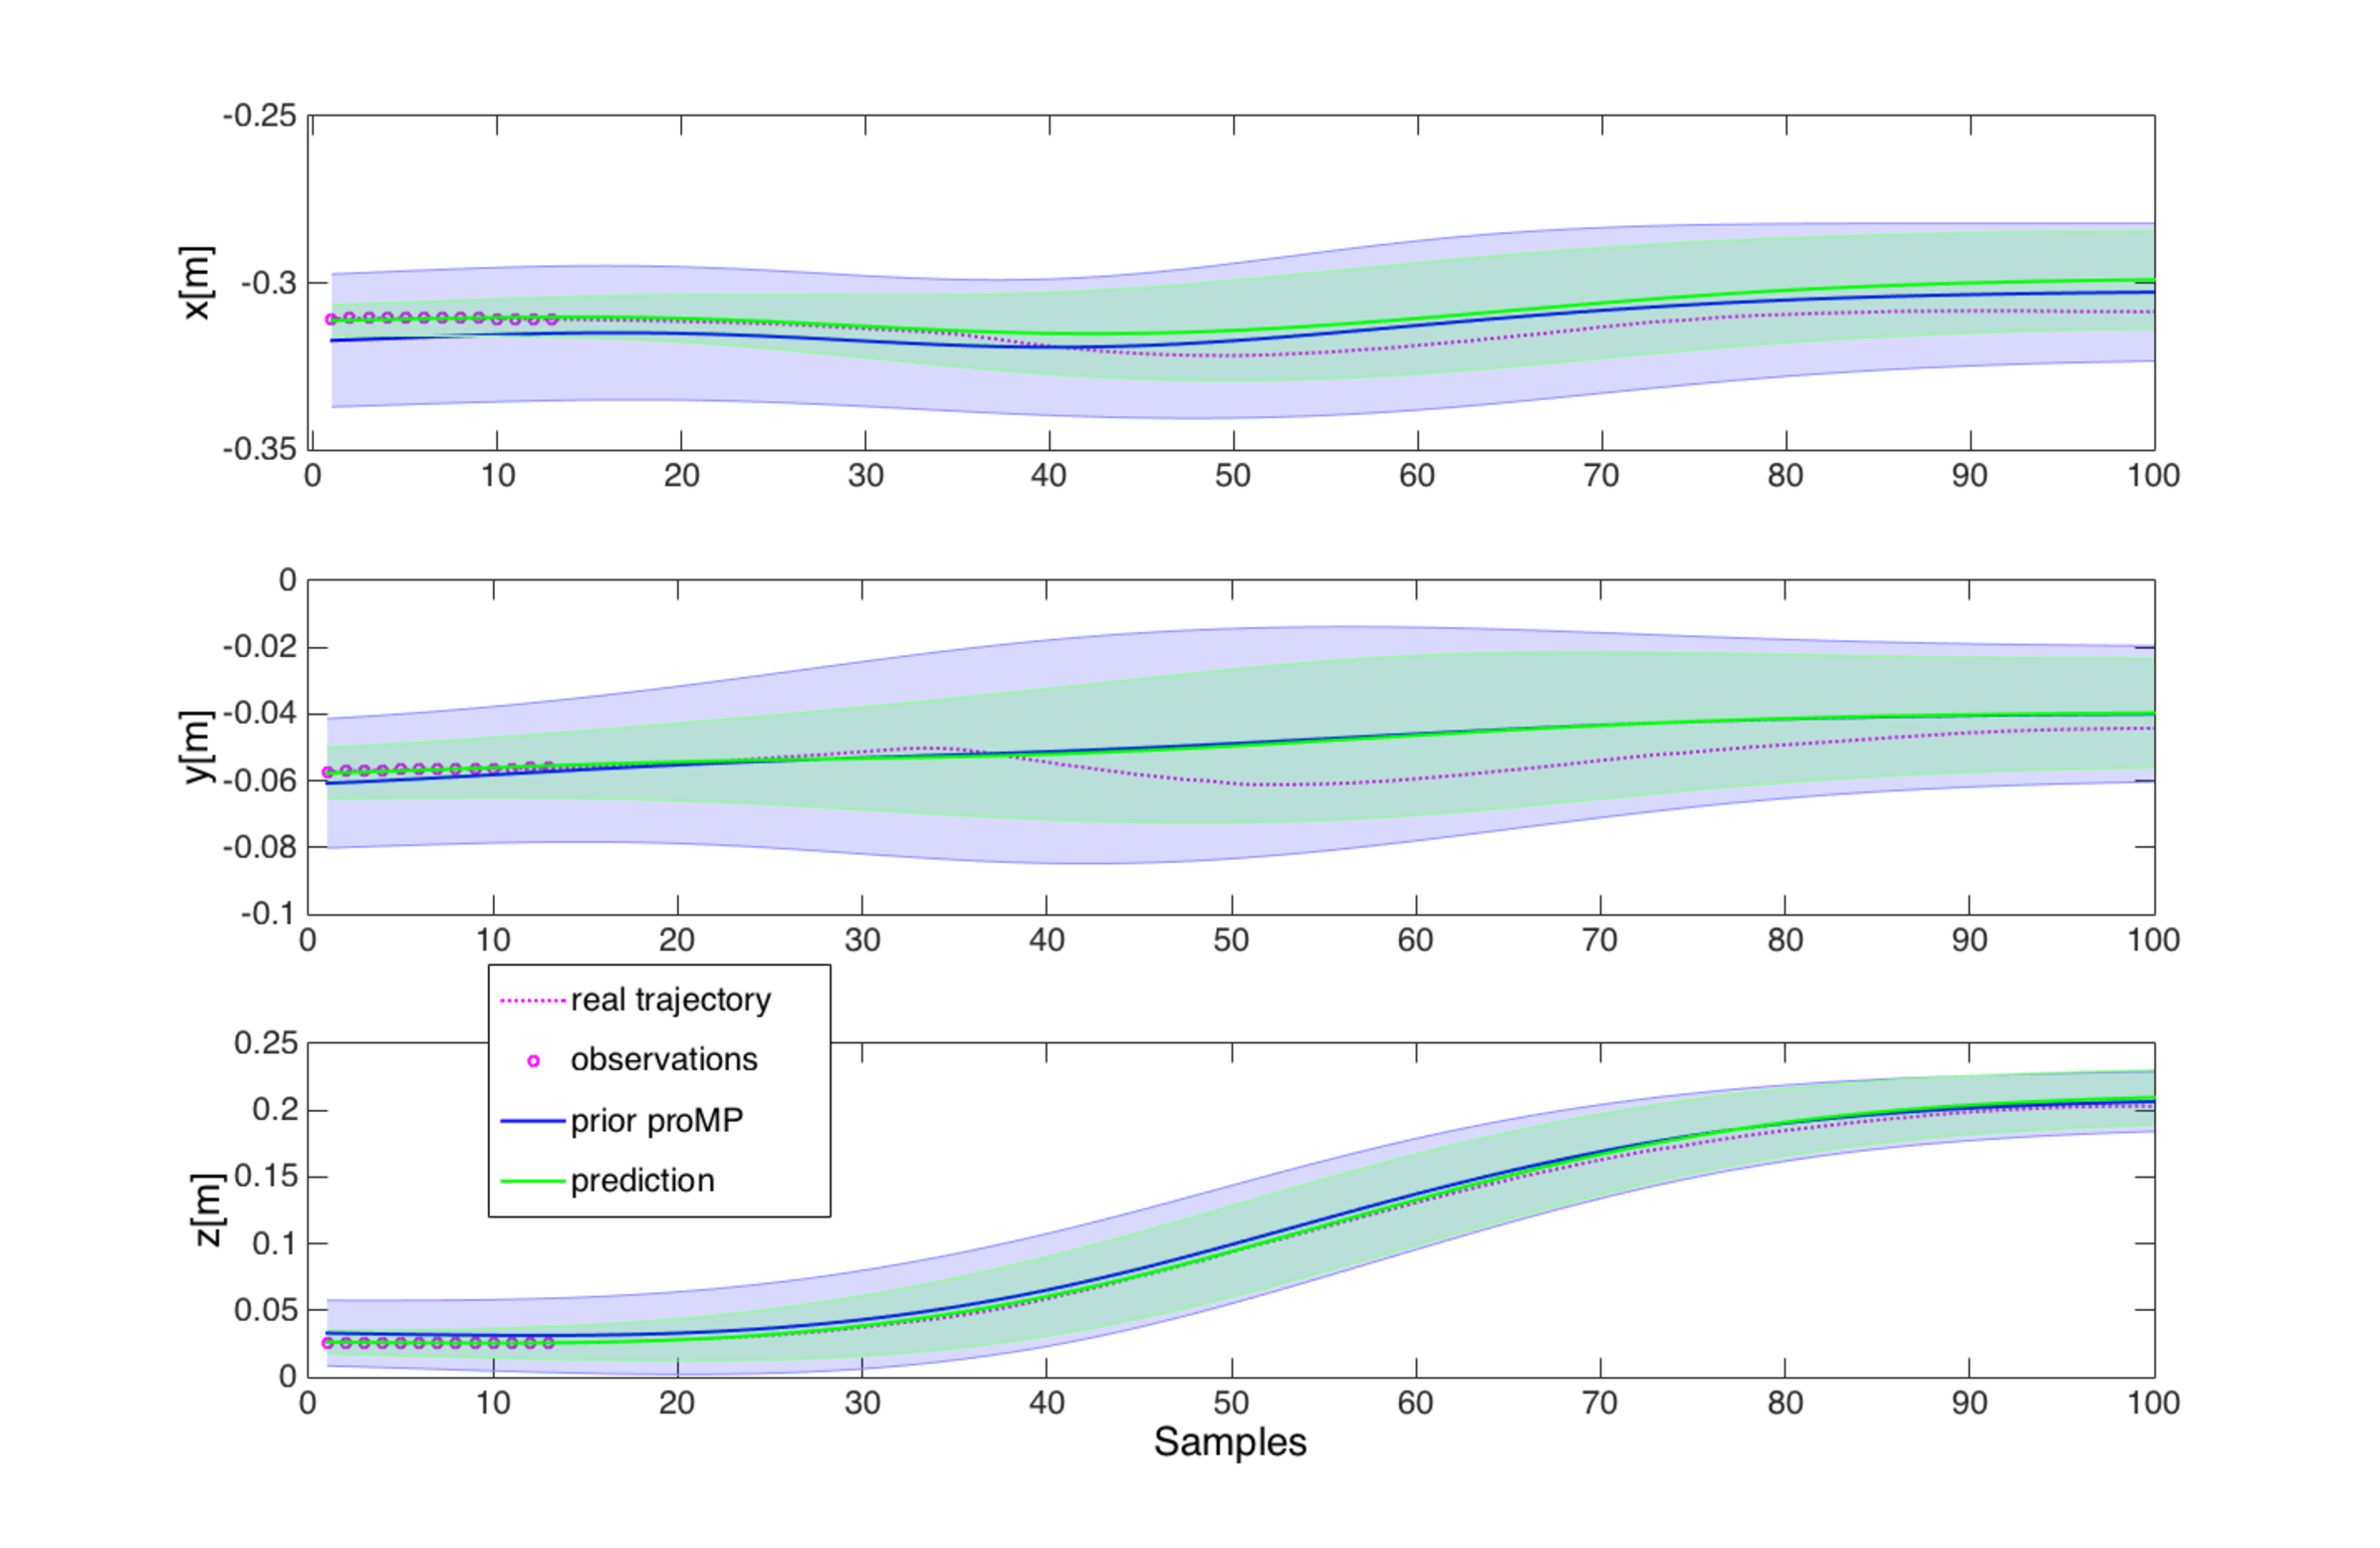
\includegraphics[height=11cm]{img/liftingWgeomagic/INFERENCE2.pdf}
%\caption{Prediction of the future trajectory, after $n_o=15$ observations, given the prior ProMP learned from $n$ demonstrations.}\todo{$/*$update the figure$*/$}
%\label{fig:predictionLifting15}
%\end{figure}

\subsection{Predicting the trajectory time modulation}\label{sec:predictDuration}
In the previous section, we presented the general formulation of ProMPs, which makes the implicit assumption that all the observed trajectories have the same duration and thus the same sampling.\footnote{Actually, we call here duration what is in fact the total number of samples for the trajectory.} That is why the duration of the trajectories generated by the RBF is fixed and equal to $\bar{s}$.
Of course, this is valid only for synthetic data and not for real data.

To be able to address real experimental conditions, we now consider the variation of the  duration of the demonstrated trajectories. 
To this end, we introduce a time modulation parameter $\alpha$ that maps the actual trajectory duration $t_{f}$ to $\bar{s}$: $\alpha = \bar{s} / t_{f}$.
%This variable rescales the RBFs of the model to the trajectory duration. 
%It relies on the trajectory duration and a reference number of samples $\bar{s}$.
The normalized duration $\bar{s}$ can be chosen arbitrarily; for example it can be set to the average of the  duration of the trajectories, \textit{e.g.}, $\bar{s}=mean(t_{f1},\ldots,t_{fK})$.
% (we have one sample per iteration time $t$).
Notably, in the literature sometimes $\alpha$ is called \textit{phase} \cite{paraschos2013probabilistic,paraschos2013probabilisticTrajectory}. 
The effect of $\alpha$ is to change the phase of the RBFs, that are scaled in time.

The time modulation of the $i$-th trajectory $\Xi_i$ is computed by $ \alpha_i = {\bar{s} \over t_{fi}}$. Thus, we have $\alpha \cdot t \in [1:\bar{s}]$. Thus, the improved ProMP model is:
\begin{eqnarray}
\xi_t = \Phi_{\alpha t} \boldsymbol{\omega} + \epsilon_t \, ,
\end{eqnarray}
where $\Phi_{\alpha t}$ is the RBFs matrix evaluated at time $\alpha t$. All the $M$ Gaussian functions of the RBFs are spread over the same number of samples $\bar{s}$. Thus, we have:
$$ \Phi_{\alpha t}=[\psi_{1}(\alpha t), \psi_{2}(\alpha t), \ldots., \psi_{M}(\alpha t)].$$
%\begin{equation}
%\Phi_{\alpha t}=[\psi_{1}(\alpha t), \psi_{2}(\alpha t), \ldots., \psi_{M}(\alpha t)] \mathrm{,~with:}  
%\psi_{i}(\alpha t) = {1 \over\sum_{j=1}^M \psi_{j}(\alpha t) }exp\{{-({\alpha t / \bar{s}} - c(i))^2 \over {2h}}\} 
%\end{equation}

%The Matlab function that allows to create such RBFs is
%
%\mcode{Phi_alpha = computeBasisFunction (s_ref,M, D, alpha, t_f, c, h,no)}
%
%\todo{Pourquoi parler ici de code???????? C est dans les sections suivantes, pas ici!!!}
%
%\begin{itemize}
%\item \mcode{s_ref} = $\bar{s}$: the reference number of samples;
%\item $M$ is the number of Gaussians of the RBFs;
%\item $D$ is the $\xi_t$ dimension;
%\item \mcode{alpha} is the time modulation parameter of $\Xi$;
%\item \mcode{t_f = s_ref / alpha} is the total time duration of $\Xi$; 
%\item \mcode{c} and \mcode{h} are the parameters of the Gaussians; 
%\item \mcode{no} informs the data number that we want to model by the RBFs (here $[1:no]$).
%\end{itemize} 
%
%The output matrix \mcode{Phi_alpha} $= \Phi_{\alpha [1:no]}$ is the RBF matrix computed to represent the first $n_o$ observed data points of a $\Xi$ trajectory.

During the learning step, we record a set of $\alpha$ parameters: $S_{\alpha} = \{\alpha_{1},\ldots,\alpha_{n}\}$.
Then, using this set, we can replay the learned ProMP with different speeds. By default (\textit{e.g.} when $\alpha=1$), the speed allows to finish the movement in $\bar{s}$ samples.


\begin{figure}[h!]
\centering
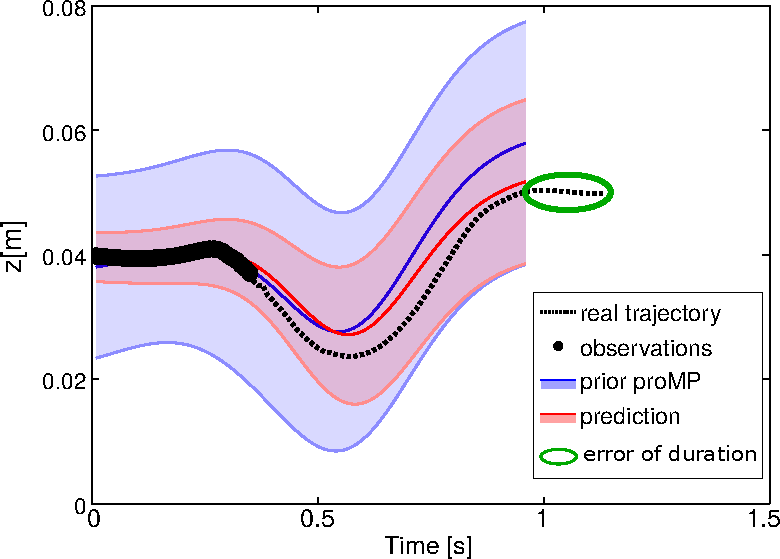
\includegraphics[width=13cm]{img/mean_alpha_errV2.pdf}
\caption{This plot shows the predicted trajectory given early observations (data points, in black), compared to the ground truth (\textit{e.g.}, the trajectory that the human intends to execute with the robot). We show the prior distribution (in light blue) and the posterior distribution (in red), which is computed by conditioning the distribution to match the observations. Here, the posterior simply uses the average $\alpha$ computed over the $\alpha_1, \ldots, \alpha_K$ of the $K$ demonstrations. Without predicting the time modulation from the observations and using the average $\alpha$, the predicted trajectory has a duration that is visibly different from the ground truth.}

\label{fig:meanAlpha}
\end{figure}

During the inference, the \rev{time modulation} $\alpha$ of the partially observed trajectory is not known. \rev{Unless fixed a priori}, the robot \rev{must} estimate it. This estimation is critical to ensure a good recognition, as shown in Figure~\ref{fig:meanAlpha}: the inferred trajectory (represented by the mean of the posterior distribution in red) 
%\todo{why "has not the same" is not correct?} 
%For Oriane: check https://english.stackexchange.com/questions/13672/have-not-versus-do-not-have
does not have the same duration as the ``real'' intended trajectory (which is the ground truth). This difference is due to the estimation error of the time modulation parameter. This estimation $\hat{\alpha}$ by default is  computed as the mean of all the $\alpha_k$ observed during the learning:
\begin{equation}
\label{eq:avg}
%\hat{\alpha} = {1 \over |S_{\alpha k}|} \sum_{\alpha \in S_{\alpha k}} \alpha
\hat{\alpha} = {{\sum \alpha_k} \over n_k} .
\end{equation}

However, using the mean value for the time modulation is an appropriate choice only when the primitive represents goal-directed motions that are very regular, or for which we can reasonably assume that differences in the duration can be neglected (which is not a general case). In many applications this estimation may be too rough.

Thus, we have to find a way to estimate the duration of the observed trajectory, which corresponds to accurately estimating the time modulation parameter $\hat{\alpha}$.
To estimate $\hat{\alpha}$, we implemented four different methods.
%Instead, we implemented simpler methods that select the most likely $\hat{\alpha}$ temporal modulation parameter according to different methods.
%\begin{itemize}
%\label{itemize:methodAlphaEstimation}
The first is the \textbf{mean of all the $\alpha_k$}, as in Equation \ref{eq:avg}. The second is
%As first method, we can simply use the \textbf{mean of the $\alpha$}:
%\begin{equation}
%\label{eq:avg}
%%\hat{\alpha} = {1 \over |S_{\alpha k}|} \sum_{\alpha \in S_{\alpha k}} \alpha
%\hat{\alpha} = {{\sum \alpha_k} \over K} .
%\end{equation}
the \textbf{maximum likelihood}, with
\begin{equation}
\label{eq:ml}
\hat{\alpha} = \mathrm{argmax}_{\alpha \in S_{\alpha k}}\{\mathrm{loglikelihood}(\Xi^o,\mu_{\boldsymbol{\omega}_k}, \sigma_{\boldsymbol{\omega}_k}, \alpha_k)\} .
\end{equation} 
The third is the \textbf{minimum distance} criterion, where we seek the best $\hat{\alpha}$ that minimizes the difference between the observed trajectory $\Xi^o_t$ and the predicted trajectory for the first $n_o$ data points:
\begin{equation}
\label{eq:minDist}
\hat{\alpha} =\mathrm{argmin}_{\alpha \in S_{\alpha k}} \{\sum_{t=1}^{{n_o}} |\Xi^o_t - \Phi_{\alpha t} \mu_{\boldsymbol{\omega}_k}|\} .
\end{equation} 
The fourth method is based on a \textbf{model}:
% \todo{find another name}: -> why changing it? the reviewers didnt mind that
we assume that there is a correlation between $\alpha$ and the variation of the trajectory $\delta_{n_o}$ from the beginning until the time $n_o$. This ``variation'' $\delta_{n_o}$ can be computed as the variation of the position, \textit{e.g.}, $\delta_{n_o} = X(n_o) - X(1)$, or the variation in the entire trajectory, $ \delta_{n_o} =\Xi(n_o) - \Xi(1)$, or any other measure of progress, if this hypothesis is appropriate for the type of task trajectories of the application.\footnote{In our case, this assumption can be appropriate, because the reaching trajectories in our application are generally monotonic increasing/decreasing.} 
Indeed, the $\alpha$ can be linked also to the movement speed, which can be roughly approximated by $\dot{X} ={ \delta X  \over t_f}$ ($\dot{\Xi} ={ \delta \Xi  \over t_f}$). We model the mapping between $\delta_{n_o}$ and $\alpha$ by: 
\begin{equation}
\label{eq:model}
\alpha = \Psi(\delta_{n_o})^\top \boldsymbol{\omega}_\alpha + \epsilon_\alpha,
\end{equation} 
where $\Psi$ are RBFs, and $\epsilon_\alpha$ is a zero-mean Gaussian noise.
During learning, we compute the  $\boldsymbol{\omega}_\alpha$ parameter, using the same method as in Equation~\ref{eq:w}.
During the inference, we compute $\hat{\alpha} = \Psi(\delta_{n_o})^\top \boldsymbol{\omega}_\alpha$.
%\end{itemize}

A comparison of the four methods for estimating $\alpha$ on a test study with iCub in simulation is presented in Section \ref{sec:simulatedTimeModulationModels}.

There exist other methods in the literature for computing $\alpha$.  For example, \cite{ewerton2015learning} propose a method that models local variability in the speed of execution. In \cite{maeda2016probabilistic} they use a method that improves Dynamic Time Warping by imposing a smooth function on the time alignment mapping using local optimization. These methods will be implemented in the future works.
%In this software, we did not implement such methods yet, since the four proposed criteria are simpler.


\subsection{Recognizing one among many movement primitives}
\label{sec:ManyProMP}
%
%we learn many movement primitives which correspond to different tasks.\\
%Let  $S_k = \{\Xi_1,\ldots, \Xi_n\}_k$, the set of trajectories that correspond to the $k$-th movement primitive.
%Let recall that $\Xi_i = [\xi_{1} \ldots \xi_{t_{fi}}]^\top$ is the $i$-th trajectory of this data set, where $t_{fi}$ is the final time of the movement. 
%
Robots should not learn only one skills, but many: different skills for different tasks. 
\rev{In our framework, tasks are represented by movement primitives, precisely ProMP.}
So it is important for the robot to be able to learn $K$ different ProMPs and then be able to recognize from the early observations of a trajectory which of the $K$ ProMPs the observations belong to.
%We are also interested in learning many ProMPs, say $K$ ProMPs.

During the learning step of a movement primitive $k \in [1:K]$, the robot observes different trajectories $S_k = \{\Xi_1,\ldots,\Xi_n\}$. For each ProMP, it learns the distribution over the parameters vector $p(\boldsymbol{\omega}) \sim \mathcal{N}(\mu_{\boldsymbol{\omega}_k}, \Sigma_{\boldsymbol{\omega}_k})$, using Equation~\ref{eq:w}. Moreover, the robot records the different phases of all the observed trajectories: $ S_{\alpha k} = \{\alpha_{1k},\ldots,\alpha_{nk}\}$.

After having learned these $K$ ProMPs, the robot \rev{can use this information to autonomously execute a task trajectory. Since we are targeting collaborative movements, performed together with a partner at least at the beginning, we want the robot to be able to recognize from the first observations of a collaborative trajectory which is the current task that the partner is doing and what is the intention of the partner. Finally, we want the robot to be able to complete the task on its own, once it has recognized the task and predicted the future trajectory. }
%\todo{why not: has to?} must finish a human-initiated movement on its own. 

Let $\Xi^{o} = [\Xi_1 \ldots \Xi_{n_o}]^\top$ be the early observations of an initiated trajectory.

From these partial observations, the robot \rev{can} recognize the \rev{``correct'' (\textit{i.e.}, most likely)} ProMP $\hat{k} \in [1:K]$.
% by:
%\begin{itemize}
\rev{First, for each ProMP $k \in [1:K]$, it computes} the most likely phase (time modulation factor) $\hat{\alpha}_k$ (as explained in Section~\ref{sec:predictDuration}), to obtain the set \rev{of ProMPs with the most likely duration}: $S_{[\mu_{\boldsymbol{\omega}_k}, \hat{\alpha}_k]} = \{(\mu_{\boldsymbol{\omega}_1},\hat{\alpha}_1),\ldots,(\mu_{\boldsymbol{\omega}_K},\hat{\alpha}_K)\}$

Then we compute the most likely ProMP $\hat{k}$ in  $S_{[\mu_{\boldsymbol{\omega}_k}, \hat{\alpha}_k]}$ \rev{according to some criterion.
One possible way is to minimize the distance between the early observations and the mean of the ProMP for the first portion of the trajectory:}
\begin{equation} \label{eq:mostlikelypromp}
\hat{k} = \arg \min_{k \in [1:K]} \,   \left[      {1 \over n_o} \sum_{t=1}^{n_o}| \Xi_{t} - \Phi_{\hat{\alpha}_k t} \, \mu_{\boldsymbol{\omega}_k} | \right]
\end{equation}
\rev{In Equation~\ref{eq:mostlikelypromp}, for each ProMP $k \in [1:K]$, we compute the average distance between the observed early-trajectory $\Xi_t$ and the mean trajectory of the ProMP $\Phi_{\hat{\alpha}_k t} \mu_{\omega_k}$, with $t = [1:n_o]$.
The most likely ProMP $\hat{k}$ is selected by computing the minimum distance (arg min). Other possible methods for estimating the most likely ProMPs could be inspired by those presented in the previous section for estimating the time modulation, \textit{i.e.} maximum likelihood or learned models.
}
%\end{itemize}
%\todo{EXPLAIN THIS EQUATION}




%Now the ProMP the most similar to the early-trajectory is identified, we can update the $\hat{k}$-th ProMP to adapt it to the observed early-trajectory.

\rev{Once identified the $\hat{k}$-th  most likely ProMP, we update its posterior distribution to take into account the initial portion of the observed trajectory, using Equation~\ref{eq:inf}:}

%The first step is then to compute $\hat{t_f}$ \rev{(the expected duration of the trajectory)} by: 
%\begin{equation}
%\hat{t_f} = \hat{\alpha_{\hat{k}}} \times \bar{s}
%\end{equation}
%The second step consists of updating the ProMP to match the early observations, using Equation~\ref{eq:inf}:

%\hat{\alpha}_{\hat{k}}
%\omega}_{\hat{k}}
\begin{equation} \label{eq:udateWithAlpha}
\left\{
\begin{array}{rl}
\hat{\mu}_{\boldsymbol{\omega}_{\hat{k}}} &= \mu_{\boldsymbol{\omega}_{\hat{k}}}  + K(\Xi^o - \Phi_{\hat{\alpha}_{\hat{k}}[1:{n_o}]}\mu_{\boldsymbol{\omega}_{\hat{k}}} ) \\ 
\hat{\Sigma}_{\boldsymbol{\omega}_{\hat{k}}}  &= \Sigma_{\boldsymbol{\omega}_{\hat{k}}}  - K(\Phi_{\hat{\alpha}_{\hat{k}}[1:{n_o}]} \Sigma_{\boldsymbol{\omega}_{\hat{k}}} ) \\
K&= \Sigma_{\boldsymbol{\omega}_{\hat{k}}} \, \Phi_{\hat{\alpha}_{\hat{k}}[1:{n_o}]}^\top \, (\Sigma_{\xi^o} + \Phi_{\hat{\alpha}_{\hat{k}}[1:n_o]}\Sigma_{\boldsymbol{\omega}_{\hat{k}}}  \Phi_{\hat{\alpha}_{\hat{k}}[1:n_o]}^\top)^{-1}
\end{array}
\right.\end{equation}
\rev{with $\hat{\alpha}_{\hat{k}}[1:n_o] = \hat{\alpha}_{\hat{k}} \, t$ (in matrix form), with $t \in [1:n_o]$.}

Finally, the inferred trajectory is given by: 
$$\forall t \in [1:\hat{t}_f], \hat{\xi}(t) = \Phi_t \, \hat{\mu}_{\boldsymbol{\omega}_{\hat{k}}}$$
with \rev{the expected duration of the trajectory $\hat{t}_f = \hat{\alpha}_k\bar{s}$.
The robot is now able to finish the movement executing the \rev{most-likely} ``future'' trajectory $\hat{\Xi} =[\hat{\xi}_{n_o+1} \ldots \hat{\xi}_{\hat{t_{f}}}]^\top$.
}

%\newpage
%%%%%%%%%%%%%%%%%%%%%%%%%%%%%%%%%%%%%%%%%%%%%%%%%%%%%%%%%%%%%%%%%%%%%%%%%%%%%%%%
\section{Software overview}\label{sec:softwareOverview}

In this section, we introduce our open-source software with an overview of its architecture. This software is composed of two main modules, represented in Figure \ref{fig:orgaSoftware}.

\label{sec:software}
\begin{figure}[h]
\center
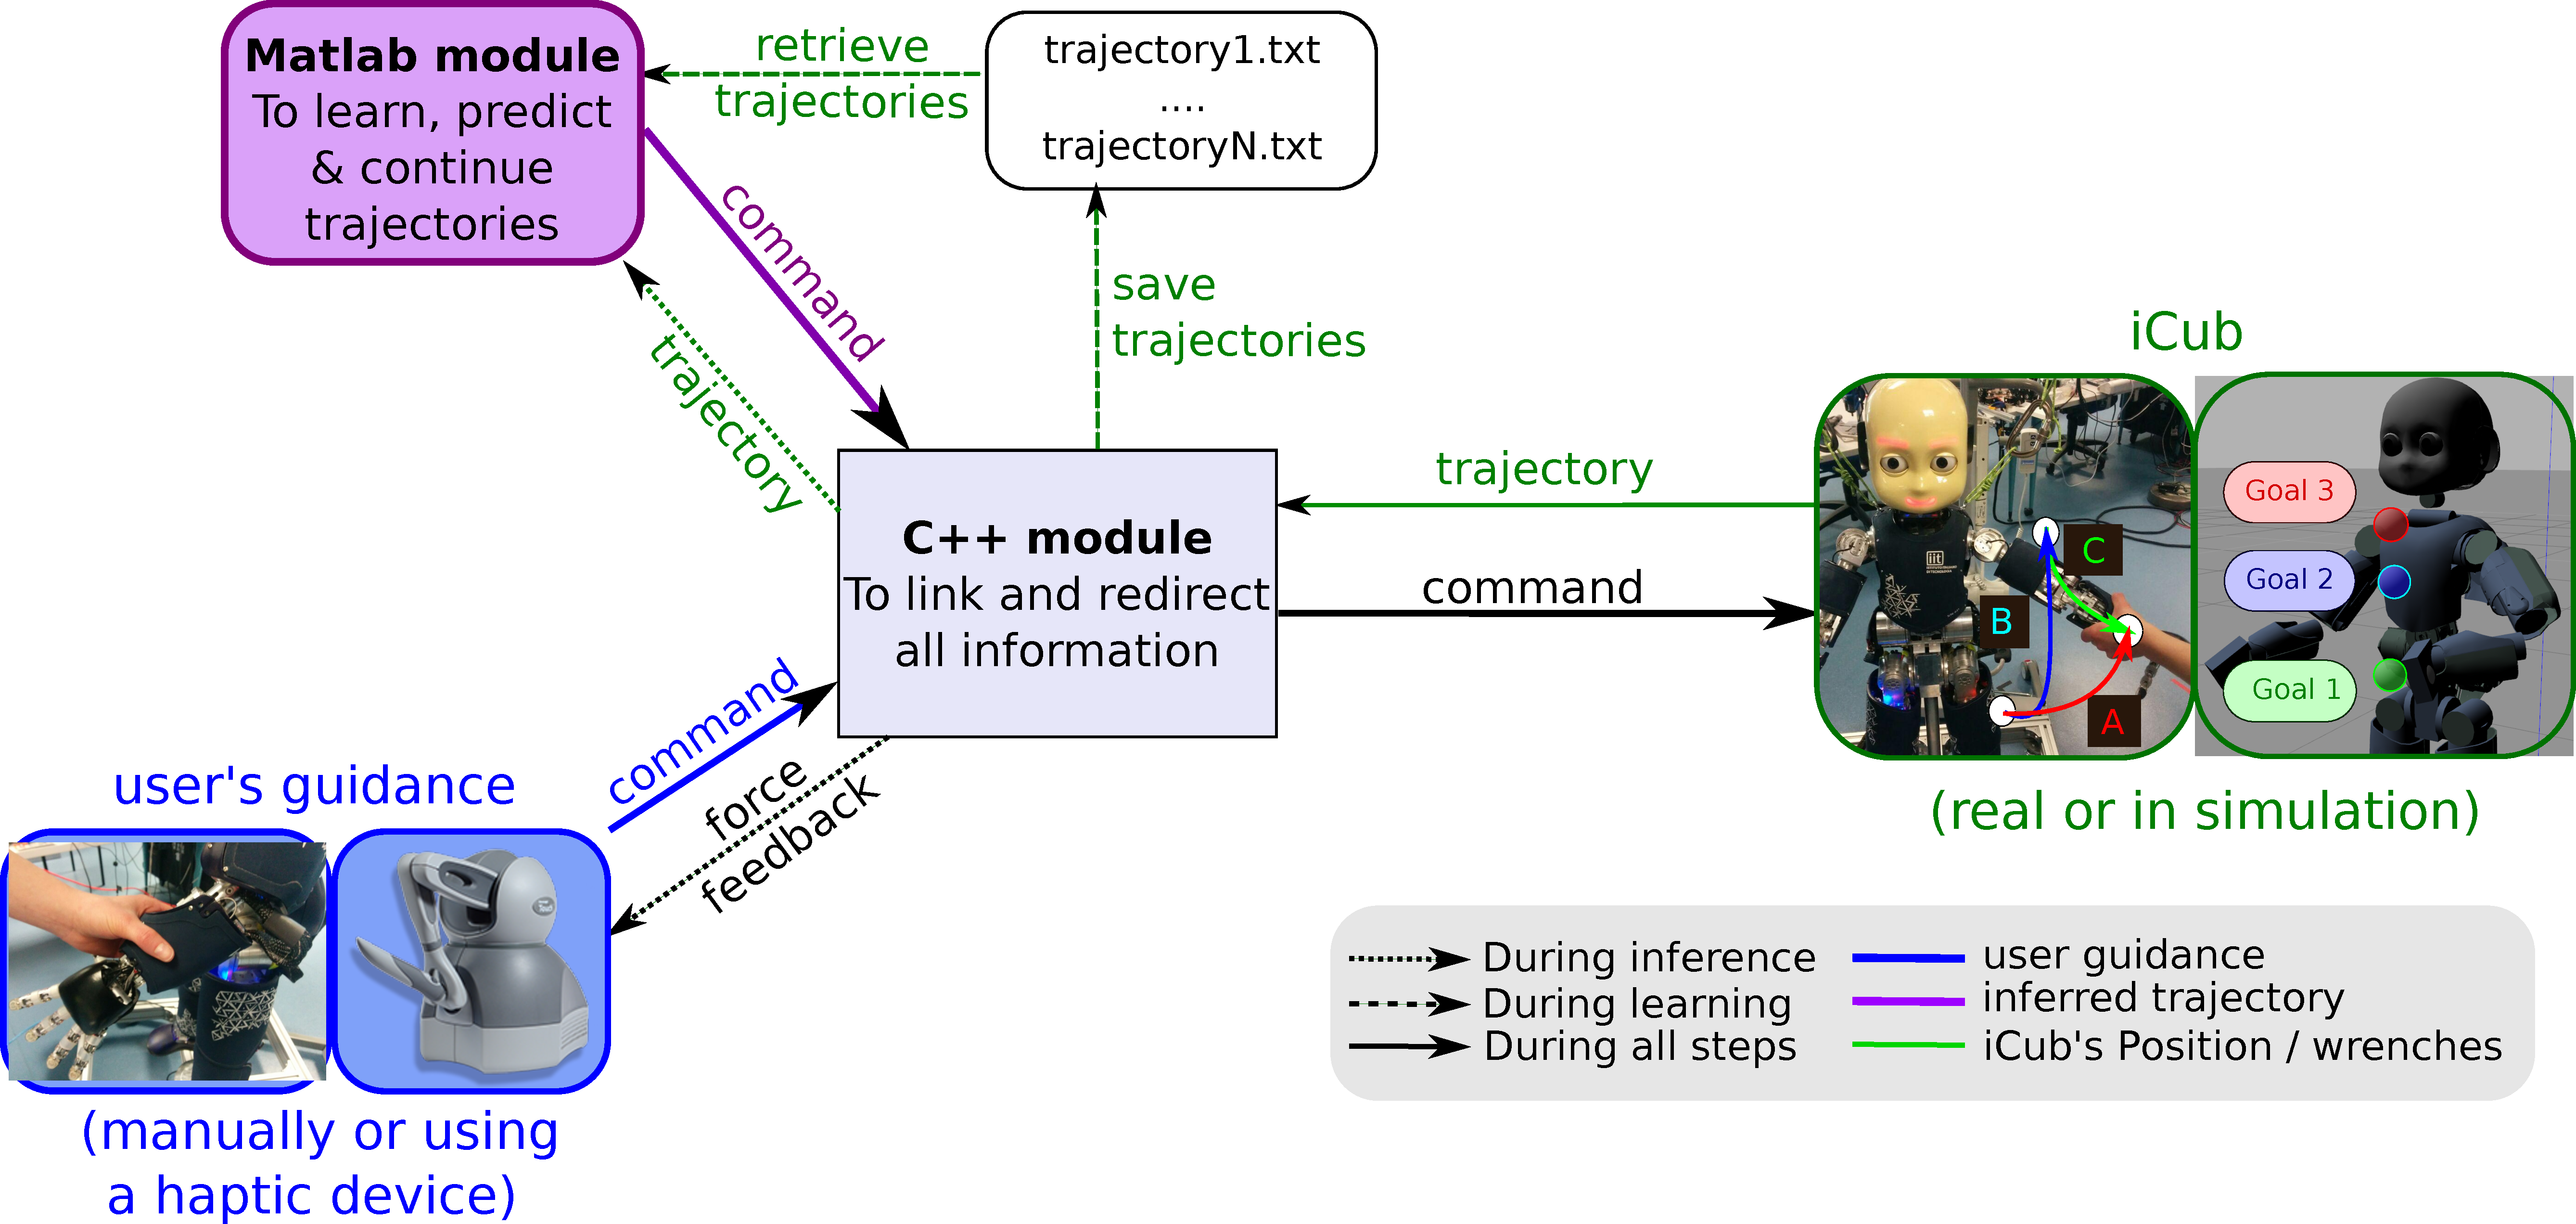
\includegraphics[width=\hsize]{img/liaisonAllProgramV3.pdf}
\caption{Software architecture and data-flows.\\ The robot's control is done either by the user's guidance (manually or through a haptic device) represented in blue, or by the Matlab module, in purple. The C++ module handles the control source to command the robot, as represented in black. Moreover, this module forwards information that comes from the iCub.}
\label{fig:orgaSoftware}
\end{figure}

\rev{While the robot is learning} the Probabilistic Movement Primitives (ProMPs) associated to the different tasks, the robot is controlled by its user. The user's guidance can be either manual for the real iCub, or through a haptic device for the simulated robot. 

\rev{A Matlab module allows replaying movement primitives or finishing a movement that has been initiated by its user}. By using this module, the robot can learn distributions over trajectories, replay movement primitives (using the mean of the distribution), recognize the ProMP that best matches a current trajectory, and infer the future evolution (until the end target) of this trajectory.
%\todo{and to make sure that the user's forces exerted on the robot are not stronger than the ones learnt.}

A C++ module forwards to the robot the control that comes either from the user or from the Matlab module. Then, the robot is able to finish a movement initiated by its user (directly or through a haptic device) in an autonomous way, as shown in Figure~\ref{fig:conceptProMP}. %\todo{This program communication also allows to correct the robot behaviour if the users forces are stronger than the expected ones.} \\

We present the C++ module in Section~\ref{subec:Setup} and the theoretical explanation of the Matlab module algorithms in Section~\ref{sec:theory}. A guide to run this last module is first presented in Section~\ref{sec:example1DOF} for a simple example, and in Section~\ref{sec:3ProMPsAppli} for our application, where a simulated robot learns many measured information of the movements. Finally, we present results on the real iCub application in Section~\ref{sec:appliRealIcub}.

Our software is available through the GPL licence, and publicly available at: 

\url{https://github.com/inria-larsen/icubLearningTrajectories}.

Tutorial, readme and videos can be found in that repository. \rev{First, the readme file describes how to launch simple demonstrations of the software. Videos present these demonstrations to simplify the understanding. In the next sections, we detail the operation of the demo program for a first case of 1DOF primitive, followed by the presentation of the specific applications on the iCub (first simulated and then real).}
%\todo{check that, it is not in the readme??}


%%%%%%%%%%%%%%%%%%%%%%%%%%%%%%%%%%%%%%%%%%%%%%%%%%%%%%%%%%%%%%%%%%%%%%%%%%%%%%%%
\section{Software example: learning a 1-DOF primitive}
\label{sec:example1DOF}
\rev{In this section, we present the use of the software to learn ProMPs in a simple case of 1-DOF primitive. This example only uses the \textit{MatlabProgram} folder, composed of:}
\begin{itemize}
\item A sub-folder called ``Data'', where \rev{there are trajectory sets used to learn movement primitives. These trajectories are stored in text files with the following information}:
%that
%\sout{there are some samples of trajectories in text files. These text files} }can be organize in various ways:
\begin{itemize}
\item [-] \textbf{input parameters}: \# input$_1$ \# input$_2$ [...]
\item [-] \textbf{input parameters with time-step}: \# timeStep \# input$_1$ \# input$_2$ [...]
\item [-] \textbf{\textit{recordTrajectories.cpp} program recording}: See Section~\ref{sec:dataAquisition} for more information.
\end{itemize}
\item A sub-folder called ``used\_functions''. It contains all the functions used to retrieve trajectories, compute ProMPs, infer trajectories, and plot results. Normally, \rev{using this toolbox does not require understanding these functions. }
%\sout{the use of this toolbox doesn't require to understand these functions}}. 
The first lines of these functions give an explanation of \rev{their} functioning and precise what are the input(s) and output(s) parameters.
\item Matlab scripts called ``demo\_*.m". They are simple examples of how to use this toolbox.
\end{itemize}

<<<<<<< HEAD
The script \mcode{demo\_plot1DOF.m}, can be used to compute a ProMP and to continue an initiated movement. The ProMP is computed from a dataset stored in a ".mat" file, called \textit{traj1\_1DOF.mat}. In this script, variables are first defined to make the script specific to the current dataset:
\begin{tabular}{|c|l|}
  \hline
  \textbf{Variable assignation} & \textbf{Commentary}\\
  \hline
  DataPath\= 'Data\/traj1\_1DOF.mat'; & Can be either ".mat" or ".txt". In the current demo,  you can also write\\
  & DataPath $=$ 'Data/traj1' if you want to use the text files of this dataset.\\
     \hline
  typeRecover= '.mat' & Or .txt, it depends on your choice of data file.\\
    \hline
  inputName = {'z[m]'}; & Label of your input(s). Here $z$ represents the $z$-axis Cartesian coordinate.\\
    \hline
  s\_ref=100; & Number of samples used as reference to rescale all the trajectories.\\
  & to the same duration.\\
    \hline
  nbInput = 1; & Dimension of the generic vector containing the state of the trajectory.\\
    \hline
  M = 5;  & Number of radial basis functions per input.\\
    \hline
  expNoise = 0.00001;  & Expected trajectory noise.\\
    \hline
  percentData = 20;  & Percent of observed data during the inference.\\
  \hline
  \end{tabular}

The variables include:
\begin{itemize}
\item \mcode{DataPath} is the path to the recorded data. If the data are stored in text files, this variable contains the folder name where text files are stored. These text files are called ``record$X$.txt", with $X \in [0:n-1]$ if there are $n$ trajectories. One folder is used to learn one ProMP. If the data are already loaded from a ``.mat" file, write the whole path with the extension. The data in ``.mat" matches with the output of the Matlab function \mcode{loadTrajectory}. %, presented in Figure~\ref{fig:yobject}.
\item \mcode{nbInput}= $D$ is the dimension of the input vector $\xi_t$. 
%This variable can be divided in two to precise in \mcode{nbInput(1)} what are the first $\xi_t$  dimensions used to recognize both the correct movement primitive and the time modulation of the initiated trajectory. In that case, \mcode{nbInput(2)}$= D - $\mcode{nbInput(1)}, contains the other dimensions, only used to compute the posterior distribution.
\item \mcode{expNoise} $= \Sigma^o_\xi$ is the expected noise of the initiated trajectory. The smaller this variable is, the stronger the modification of the ProMP distribution will be, given new observations.
\end{itemize}

%\rev{After this variable declaration, the user can just launch the script. To give a deeper understanding of this script, we now detail which and how functions are called in it.} 
We will now explain more in detail the script. 
To recover data recorded in a ``.txt'' file, we call the function:

\mcode{t\{1\} = loadTrajectory(PATH, nameT, varargin)} 

Its input parameters specify the path of the recorded data, the label of the trajectory. Other information can be added by using the \mcode{varargin} variable (for more detail, check the header of the function with the help comments). 
%For more detail about these parameters, read the beginning of this function. 
The output is an object that contains all the information about the demonstrated trajectories. \rev{It is composed of \mcode{nbTraj}, the number of trajectory; \mcode{realTime}, the simulation time; \mcode{y} (and \mcode{yMat}), the vector (and matrix) trajectory set , etc.}. 
%\rev{\sout{Note that to simplify the Matlab's notation, we denote the $\Xi$ trajectory by \mcode{y} (or \mcode{yMat} in all the toolbox functions}}. 
\rev{Thus, \mcode{t\{1\}.y\{i\} } contains the $i$-th trajectory}.

%\begin{figure}[h]
%\centering
%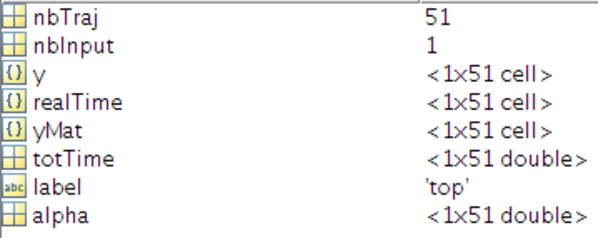
\includegraphics[height=4cm]{img/yobject.pdf}
%\caption{Object that contains information about 51 observed trajectories of a 1DOF movement primitive.}
%\label{fig:yobject}
%\end{figure}

The Matlab function \mcode{drawRecoverData(t\{1\}, inputName,'namFig', nFig, varargin)} plots in a Matlab figure (numbered \mcode{nFig}) the dataset of loaded trajectories. %By lack of place, we don't represent here these trajectories.
\rev{An example is shown in Figure~\ref{fig:1DOFtrajectoriesProMP}, on the left. Incidentally, the different duration of the trajectories is visible: on average, it is $1.17 \pm 0.42$ seconds.}

% a plot such as Figure~\ref{fig:1DOFtrajectories}. In this Figure, the average duration of these trajectories is $1.17 \pm 0.42$ seconds.

%\begin{figure}[h]
%\centering
%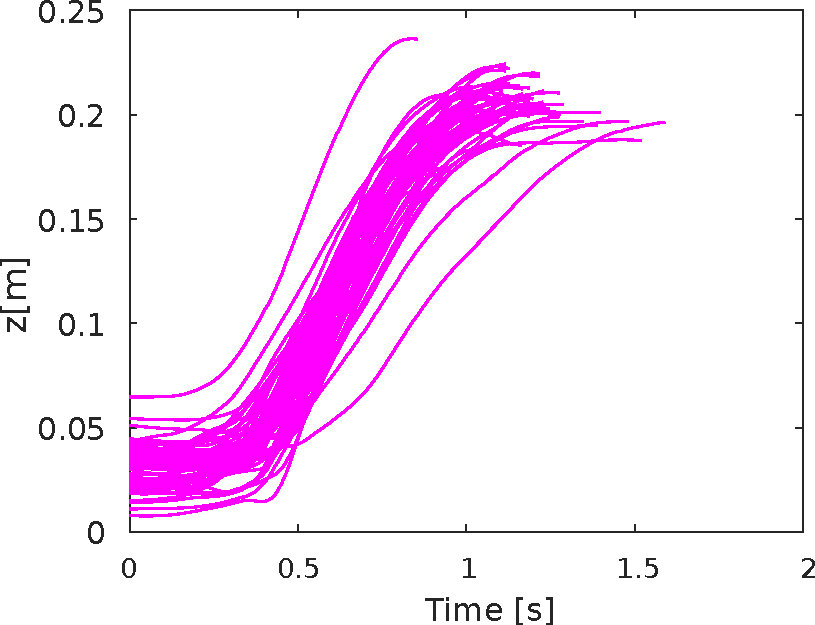
\includegraphics[height=8cm]{img/1DOFtrajectoriesV2.pdf}
%\caption{The trajectories of the test dataset for 1DOF primitive.}
%\label{fig:1DOFtrajectories}
%\end{figure}

To split the \rev{entire dataset of demonstrated} trajectories \mcode{t\{1\}} 
into a training dataset (used for learning the ProMPs) and a test dataset (used for the inference), call the function

\mcode{[train, test] =  partitionTrajectory(t\{1\}, partitionType, percentData, s_ref)}
\rev{where if \mcode{partitionType}$=1$, only one trajectory is in the test set and the others are placed in the training set, and if \mcode{partitionType}$ >1$ it corresponds to the percentage of trajectories that will be included in the training set.} 
%\rev{\sout{
%where \mcode{percentTrain} is the percentage of trajectories that \rev{will be included \sout{goes}} in the training \rev{\sout{data}}set. If \mcode{percentTrain=1}, only one trajectory is randomly selected to be in the inference dataset.}}

\rev{The ProMP can be computed from the training set by using the function}:

\mcode{promp = computeDistribution(train, M, s_ref,c,h)}

The output variable \mcode{promp} is an object that contains all the ProMP information. 
The first three input parameters have been presented before: \rev{\mcode{train} is the training set, \mcode{M} is the number of RBFs, \mcode{s_ref} is the number of samples used to rescale all the trajectories.}
The last two input parameters \mcode{c} and \mcode{h} shape the RBFs of the ProMP model: \mcode{c} $\in \mathbb{R}^M$ is the center of the Gaussians and \mcode{h} $\in \mathbb{R}$ their variance. 

%In Matlab, the equivalent code is:
%\begin{lstlisting}
%for i = 1:3
%	if i >= 5 && a ~= b       % literate programming replacement
%		disp('cool');           % comment 
%	MATLAB CODE
%end
%\end{lstlisting}
%\todo{I don't get here what you want I write: to c/p the program will be to long. DO you want I do a pseudo-code?}
To visualize this ProMP, as shown in Figure~\ref{fig:1DOFtrajectoriesProMP}, call the function:
\mcode{drawDistribution(promp, inputName,s_ref)}



\begin{figure}[h]
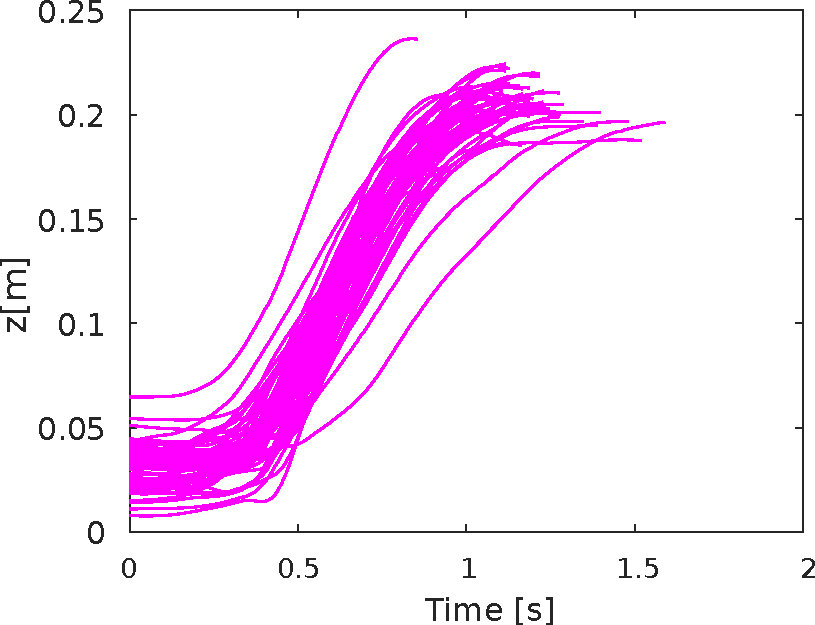
\includegraphics[width=\hsize /2]{img/1DOFtrajectoriesV2.pdf} 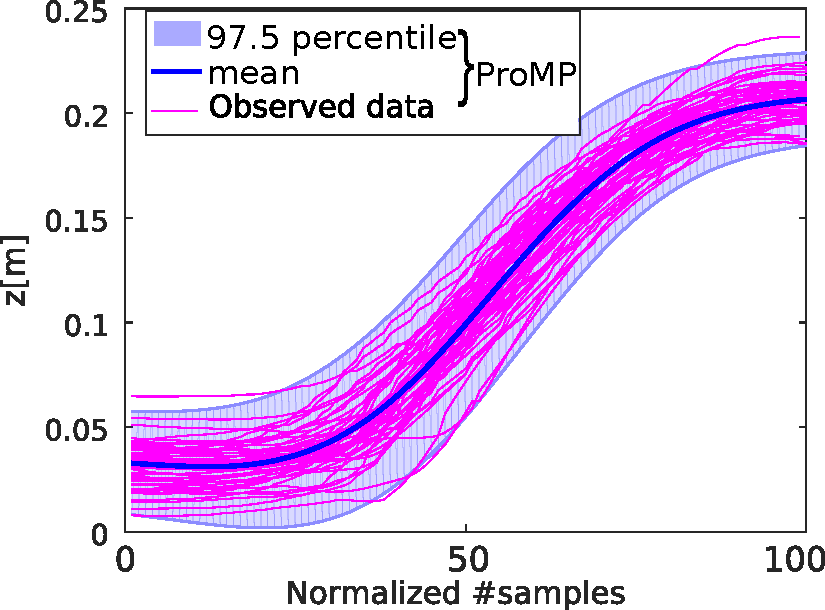
\includegraphics[width=\hsize /2]{img/1DOFtrajectoriesProMPV2.pdf}
%\caption{The trajectories of the test dataset for 1DOF primitive.}
\caption{The observed trajectories are represented in magenta. The corresponding ProMP is represented in blue. The following parameters are used: $\bar{s}=100$ for the reference number of samples, $M=5$ for the number of RBFs spread over time, and  $h=0.04$ (=$ 1 \over M^2$) the variance of the RBFs.}
\label{fig:1DOFtrajectoriesProMP}
\end{figure}

%In this figure, the distribution is represented according to a reference number of samples $\bar{s} = 100$, and the observed trajectory are resaled according to this number of samples, to facilitate the understanding.

For debugging purposes and to understand how to tune the ProMPs' parameters, it is interesting to plot the overlay of the basis functions in time. Choosing an appropriate number of basis functions is important, as too few may be insufficient to approximate the trajectories under consideration, and too many could result in over-fitting problems.
To plot the basis functions, simply call: 

\mcode{drawBasisFunction(promp.PHI,M)}

where \mcode{promp.PHI} is a set of RBFs evaluated in the normalized time range $t \in [1:\bar{s}]$.
%, each of which being evaluated at a different time $t \in [1:\bar{s}]$. \todo{is it better?}%during the interval: $\Phi_{[1:\bar{s}]}$ \todo{reformulate this}. 

Figure \ref{fig:1DOFtrajectoriesProMPbasis} shows at the top the basis functions before normalization, and at the bottom the ProMP modeled from these basis functions. From left to right, we change the number of basis functions. When there are not enough basis functions (left), the model is not able to correctly represent the shape of the trajectories. In the middle, the trajectories are well represented by the five basis functions. With more basis functions (right), the variance of the distribution decreases because the model is more accurate. 
\rev{However, arbitrarily increasing the number of basis functions is not a good idea, as it may not improve the accuracy of the model and worse it may cause overfitting. }
%\rev{With too many basis function, there is no real improvement of the accuracy and it may be overfitting}.
%As a balance, the computation time increases.

\begin{figure}[h]
\centering
{
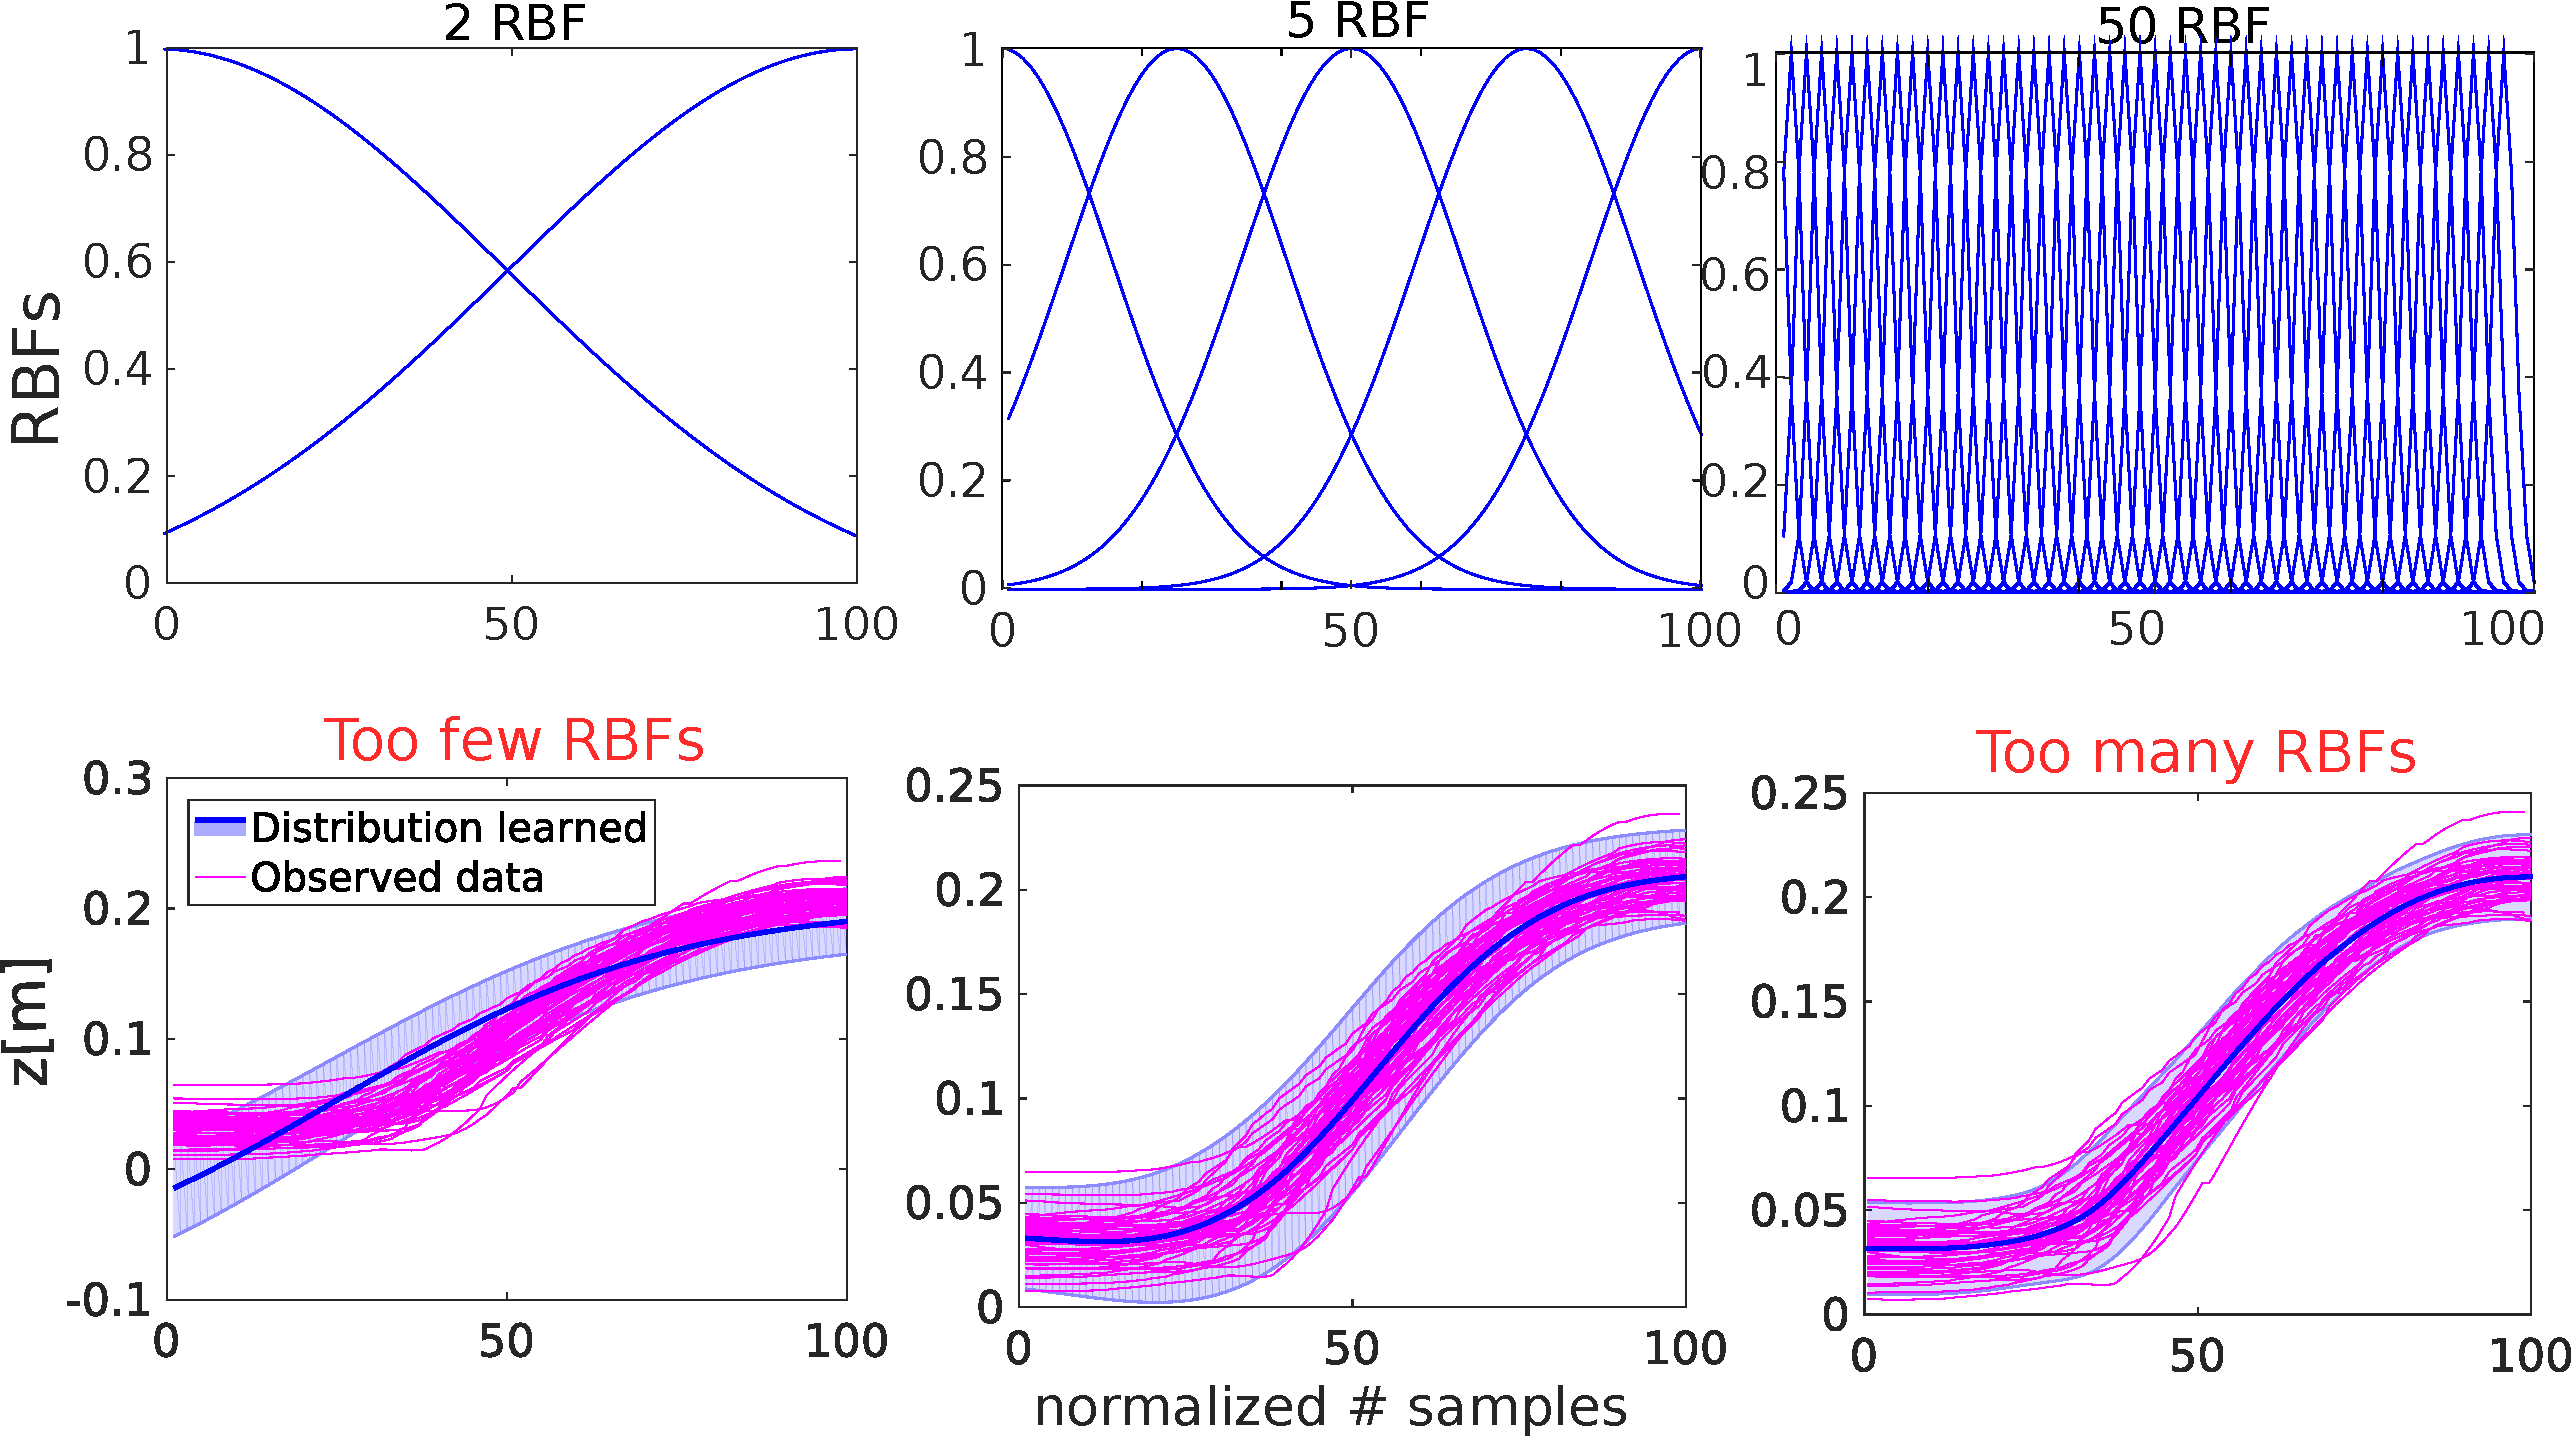
\includegraphics[width=\hsize]{img/1DOFtrajectoriesProMPbasisV4.pdf}
}
\caption{The ProMP computed for the test dataset (Figure \ref{fig:1DOFtrajectoriesProMP}) using different numbers of basis functions: from left to right: $M=\{2,5,50\}$ basis functions before normalization, with a variance $h={1 \over M^2}$. }
\label{fig:1DOFtrajectoriesProMPbasis}
\end{figure}

Once the ProMP is learned, the robot can reproduce the movement primitive using the mean of the distribution.
Moreover, it can now recognize a movement that has been initiated in this distribution, and predict how to finish it. To do so, given the early $n_{o}$ observations of a movement, the robot updates the prior distribution to match the early observed data points: through conditioning, it finds the posterior distribution, that can be used by the robot to execute the movement on its own.

The first step in predicting the evolution of the trajectory is to infer the duration of this trajectory, which is encoded by the time modulation parameter $\hat{\alpha}$. The computation of this inference, which was detailed in Section~\ref{sec:predictDuration}, can be done by using the function:

\mcode{[expAlpha,type,x]=inferenceAlpha(promp,test\{1\},M,s_ref,c,h,test\{1\}.nbData, expNoise, typeReco)}

where \mcode{typeReco} is the type of criteria used to find the expected time modulation ('MO', 'DI' or 'ML' for model, distance or maximum likelihood methods); \mcode{expAlpha} $=\hat{\alpha}$ is the expected time modulation; \mcode{type} is the index of the ProMP from which \mcode{expAlpha} has been computed, which we note in this paper as $k$ .
%\mcode{x} is used for debugging purpose.
%\marco{Finally \mcode{x = test\{1\} + offset} is the trajectory transposed by an offset, to be centred on the mean of the recognized ProMP at time $t=1$ (only used for debugging purposes).[Obs.: I didn’t understand
%584 this.] }
%\rev{it is hard to explain in the paper, but from the early-trajectory, to recognize which ProMPs correspond the best to the initiated trajectory, I need to translate the early-trajectory to compute how likely the "shape" of the early-trajectory correspond to the ProMP}
To predict the evolution of the trajectory, we use Equation~\ref{eq:inf} from Section \ref{sec:predict}. In Matlab, this is done by the function:
\mcode{infTraj = inference(promp, test\{1\}, M, s_ref, c, h, test\{1\}.nbData, expNoise, expAlpha)}\\
where \mcode{test\{1\}.nbData} has been computed during the \mcode{partitionTrajectory} step. This variable is the number of observations $n_o$, representing the percentage of observed data (\mcode{percentData}) of the test trajectory (\textit{i.e.}, to be inferred) that the robot observes. \mcode{infTraj}$= \hat{\Xi}$ is the inferred trajectory.
Finally, to draw the inferred trajectory, we can call the function  \mcode{drawInference(promp,inputName,infTraj, test{1},s_ref)}.

It can be interesting to plot the quality of the predicted trajectories as a function of the number of observations, as done in Figure \ref{fig:1DOFtrajectoriesPredictions}.

\begin{figure}[h]
\centering
{
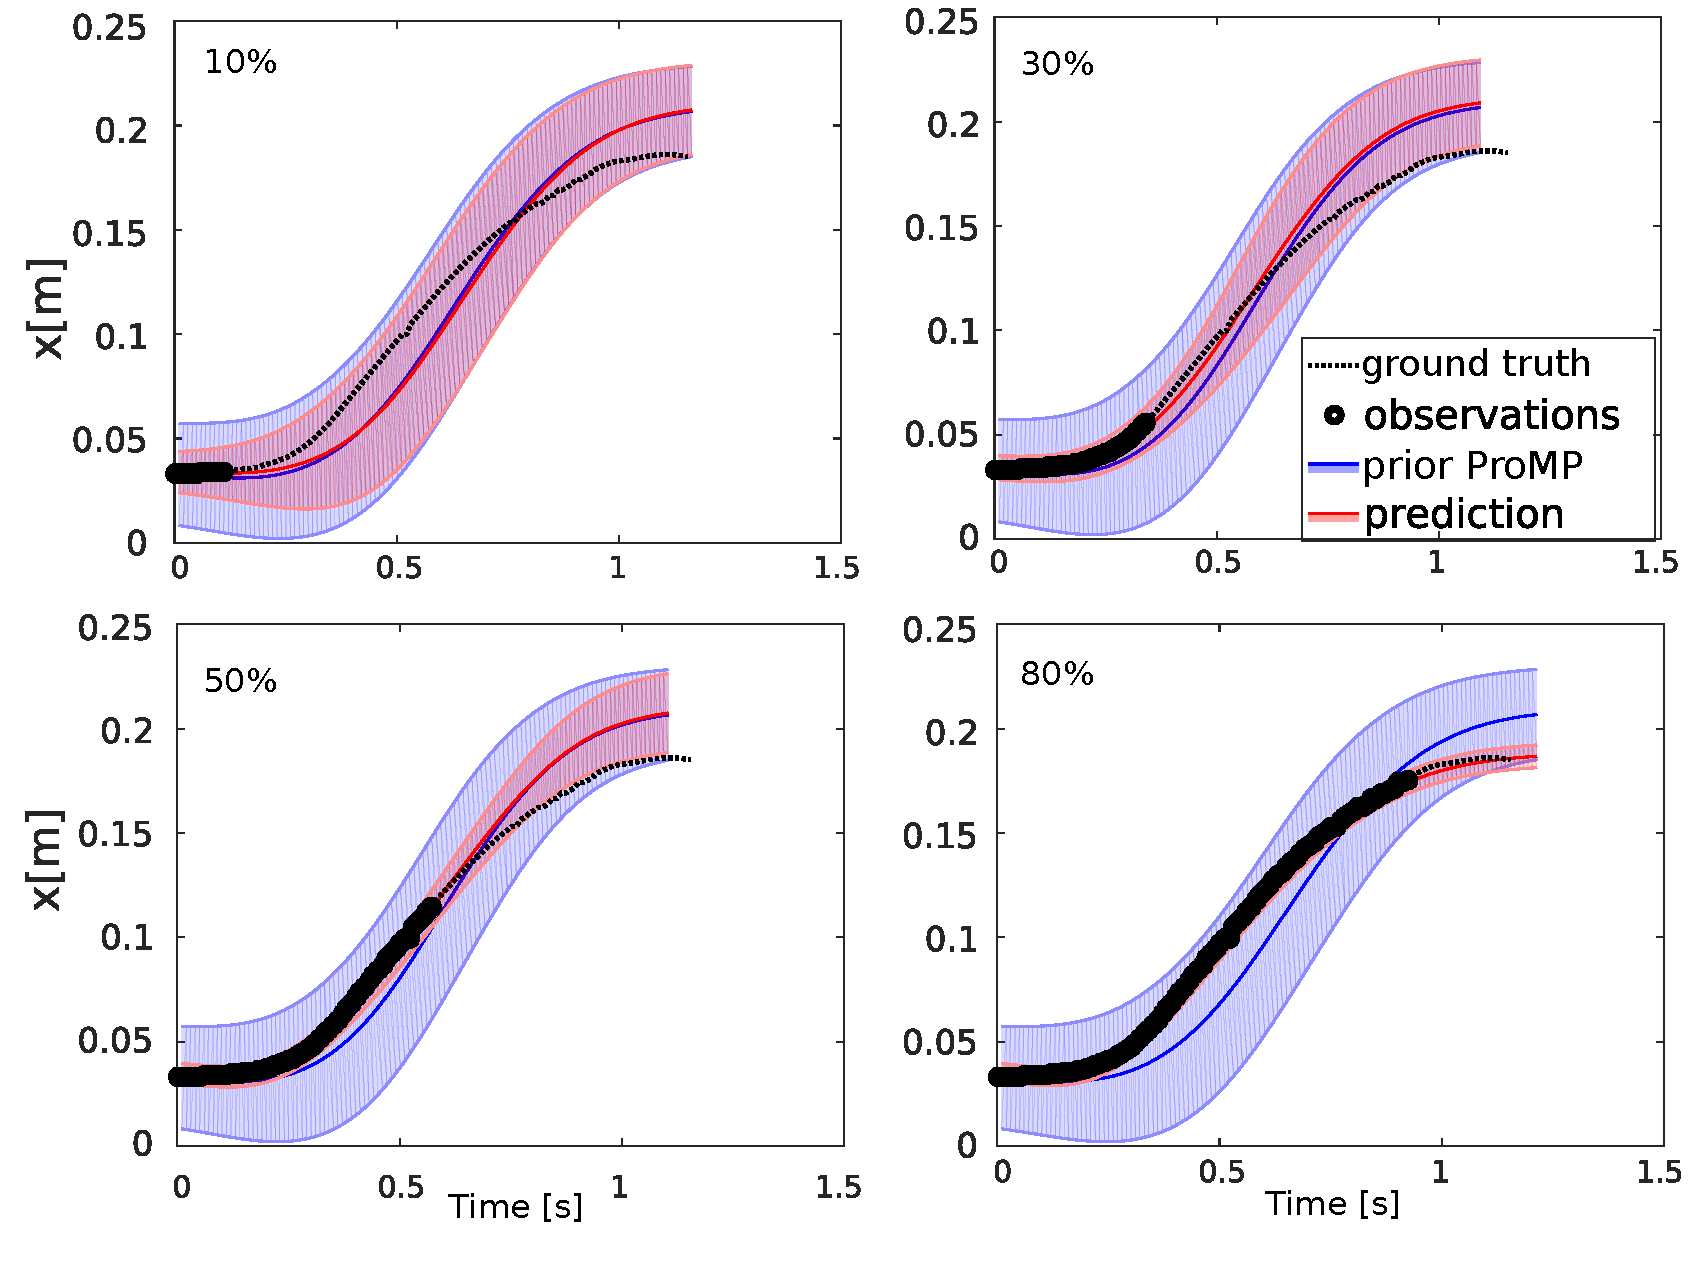
\includegraphics[width=15cm]{img/1DOFtrajectoriesPredictionsV2.pdf}
}
\caption{The prediction of the future trajectory given early observations, exploiting the information of the learned ProMP (Figure \ref{fig:1DOFtrajectoriesProMP}). The plots show the predicted trajectories after 10\%, 30\%, 50\% and 80\% of observed data points.}
% \marco{[This paper explained how to compute the posterior over $\omega$, but not how to
%compute the prior nor the posterior over trajectories. However this must be computed somewhere
%to generate figures such as this one.]} \rev{I don't understand, in eq~\ref{eq:w} we explain how the prior is computed}}
\label{fig:1DOFtrajectoriesPredictions}
\end{figure}

Note that when we have \rev{observed a larger portion of the trajectory, the prediction of the remaining portion is more accurate}.

Now we want to measure the quality of the prediction. Let $\Xi^* = [\xi^o(1),\ldots, \xi^o({n_o}), \xi^*(n_o+1),\ldots, \xi^*(t^*_f)]$ be the real trajectory expected by the user. 
To measure the quality of the prediction, we can use:
\begin{itemize}
\item The likelihood of having the $\Xi^*$ trajectory given the updated distribution $\hat{p(\boldsymbol{\omega})}$.
\item The distance between the $\Xi^*$ trajectory and the  $\hat{\Xi}$ inferred trajectory.
\end{itemize}

However, according to the type of recognition \mcode{typeReco} used to estimate the time modulation parameter $\alpha$ from the early observations, a visible mismatch between the predicted trajectory and the real one can be visible even when a lot of observations are used. This is due to the error of the expectation of this time modulation parameter. In Section \ref{sec:predictDuration}, we present the different methods used to predict the trajectory duration. These methods select the most likely $\hat{\alpha}$ according to different criteria: distance; maximum likelihood; model of the $\alpha$ variable\footnote{In this model, we assume that we can find the time modulation parameter according to the global variation of the position during the $n_o$ first observed data.}; and average of the observed $\alpha$ during learning.
%
%\todo{Je ne pense pas mettre l'exemple ci dessous que tu souhaitais parce que le code est assez long. \\
%In Matlab, this further prediction can be done by:}
%
%\begin{lstlisting}
%for i = 1:3
%	if i >= 5 && a ~= b       % literate programming replacement
%		disp('cool');           % comment 
%	MATLAB CODE
%end
%\end{lstlisting}

Figure \ref{fig:1DOFtrajectoriesPredictionsDuration} shows the different trajectories predicted after $n_{o}=40\%$ of the length of the desired trajectory is observed, according to the method used to estimate the time modulation parameter. 

On this simple test, where the variation time is little as shown in Table \ref{tab:alphaProMP}, the best result is accomplished by the average of time modulation parameter of the trajectories used during the learning step. In more complicated cases, when the time modulation varies, the other methods will be preferable as seen in Section~\ref{sec:ManyProMP}.
\begin{table}
\center
\begin{tabular}{|p{2.5cm}|p{2.5cm}|p{4.5cm}|p{2.5cm}|}
  \hline
    & Traj. Samples & $\alpha = {\bar{s} \over \mathrm{Iterations}}, \bar{s}=100$ & Duration [s] \\
     \hline
     Min & 83 & 1.2048 & 0.83 \\
     \hline
     Max & 115 & 0.8696 & 1.15\\
     \hline
     Mean & 100& 1& 0.99 \\
     \hline
     Std deviation & 9 & 11.1111 & 0.09 \\
     \hline
\end{tabular}
\caption{information about trajectories' duration}
\label{tab:alphaProMP}
\end{table} 

\begin{figure}[h]
\centering
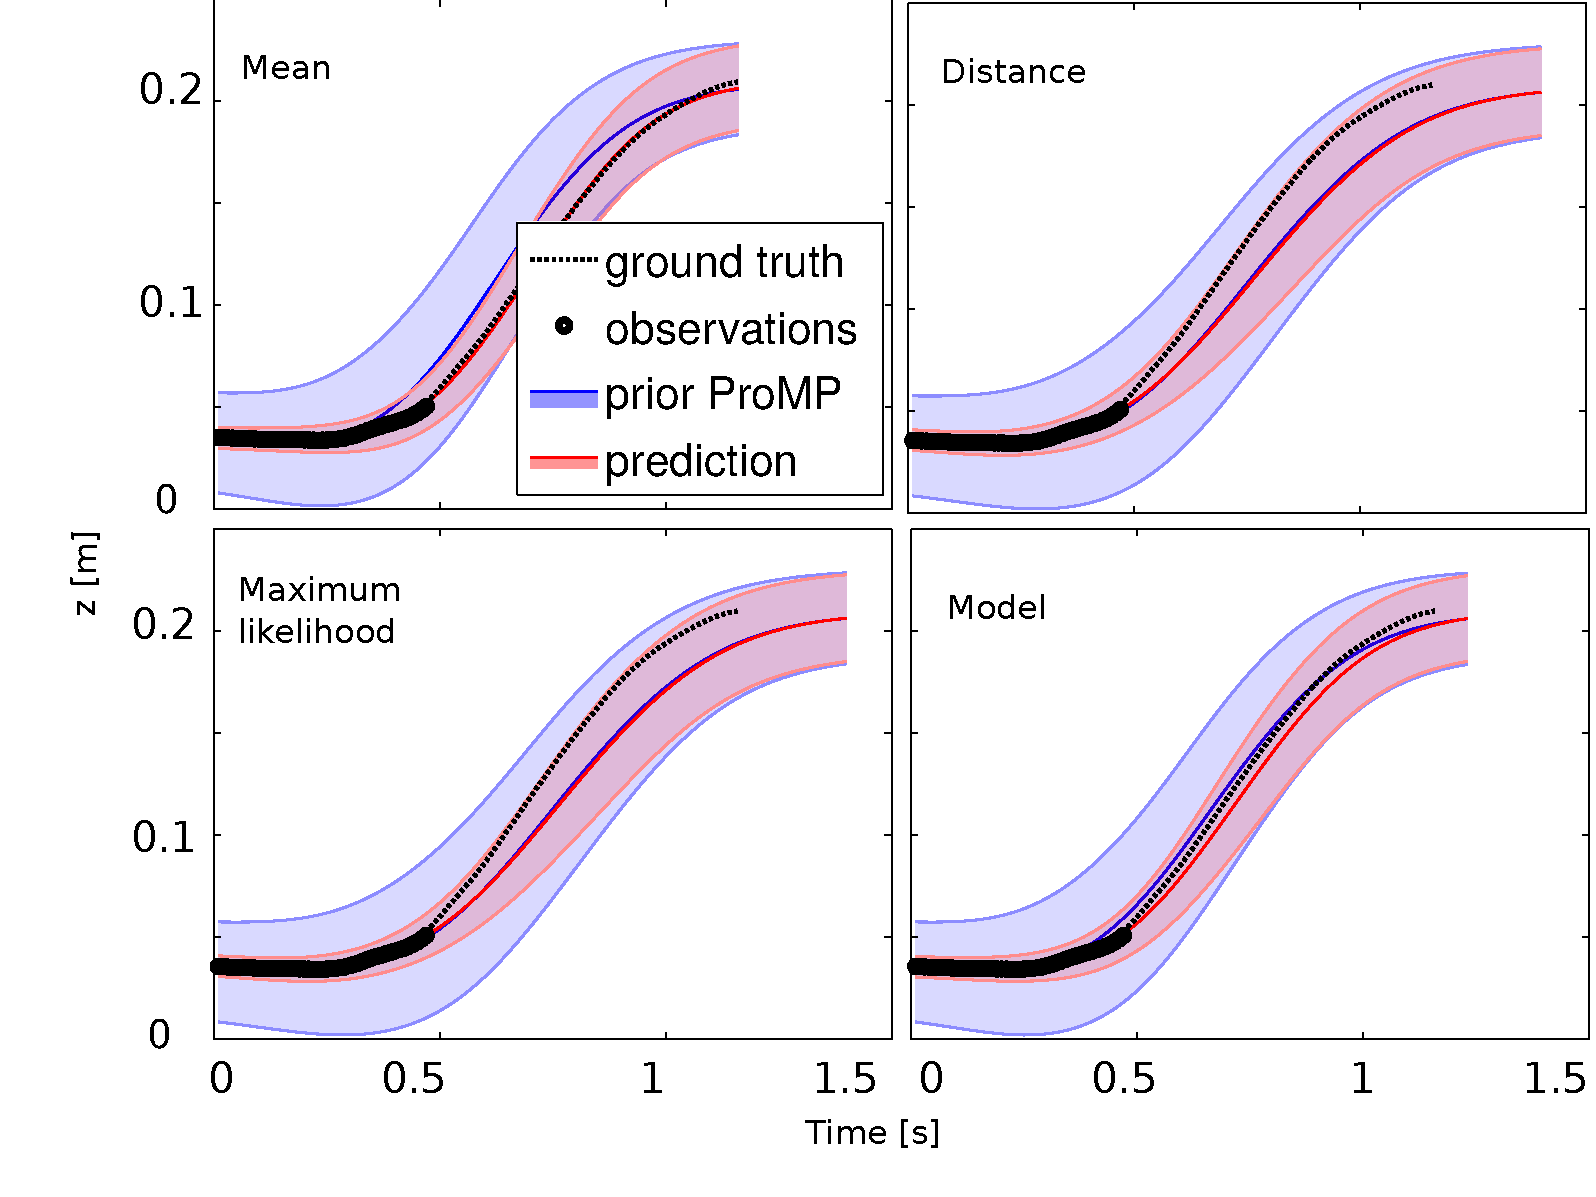
\includegraphics[width=15cm]{img/1DOFtrajectoriesPredictionsDurationV2.pdf}
\caption{The prediction of the future trajectory given $n_{o}=40\%$ of early observations from the learned ProMP computed for the test dataset (Figure \ref{fig:1DOFtrajectoriesProMP}). The plots show the predicted trajectory, using different criteria to estimate the best phases of the trajectory: using the average time modulation (Equation~\ref{eq:avg}); using the distance criteria (Equation~\ref{eq:minDist}); using the maximum log-likelihood (Equation~\ref{eq:ml}); or using a model of time modulation according to the time variation (Equation~\ref{eq:model}).}
\label{fig:1DOFtrajectoriesPredictionsDuration}
\end{figure}


%%%%%%%%%%%%%%%%%%%%%%%%%%%%%%%%%%%%%%%%%%%%%%%%%%%%%%%%%%%%%%%%%%%%%%%%%%%%%%%%
\section{Application on the simulated iCub: learning three primitives}
\label{sec:3ProMPsAppli}
\begin{figure}[h]
\centering
{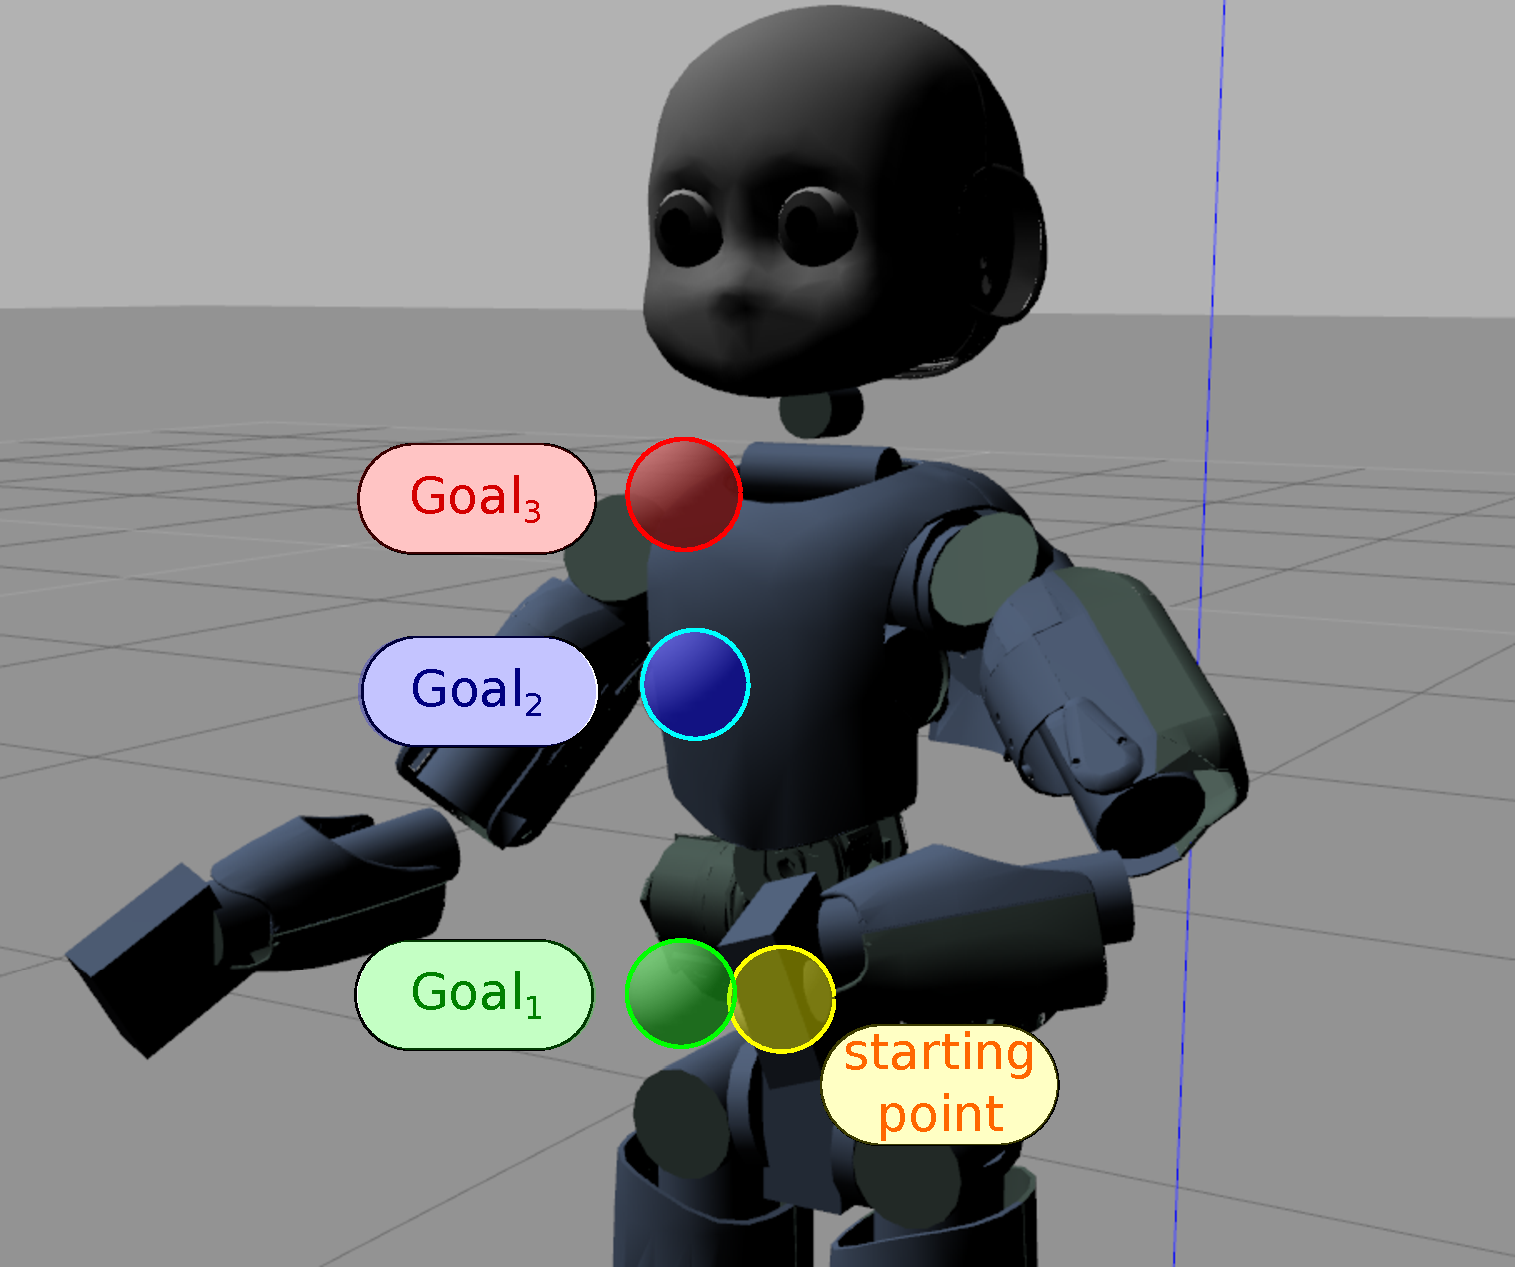
\includegraphics[width=8cm]{img/gazeboGoalsV2.pdf}
\hspace{0.1cm}
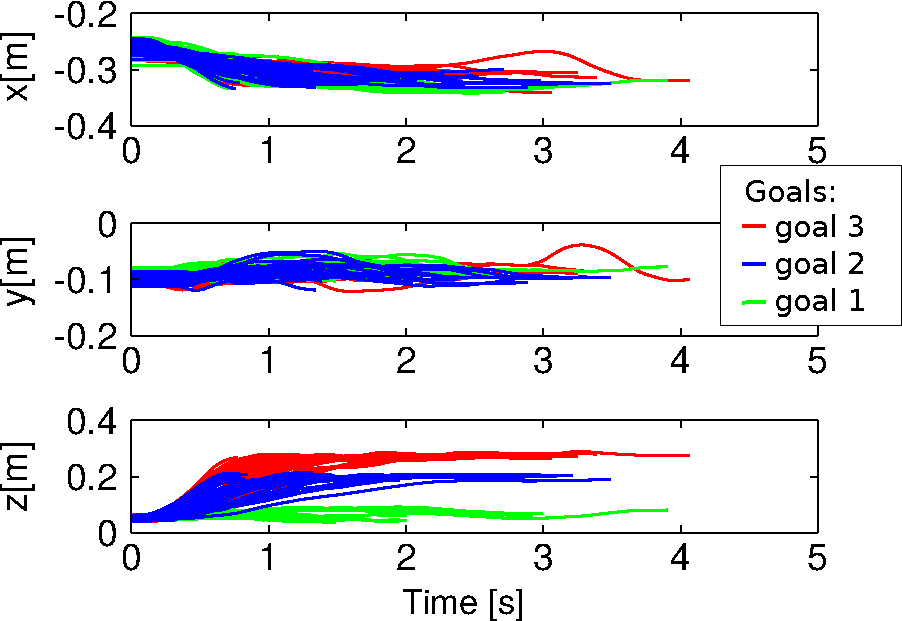
\includegraphics[width=9cm]{img/3DOFtrajectories.pdf}
}
\caption{Left: the three colored targets that the robot must reach from the starting point; the corresponding trajectories are used to learn three primitives representing three skills. 
Right: the Cartesian position information of the demonstrated trajectories for the three reaching tasks.}% trajectories x (top),y(middle) and(bottom) without force information that are also recorded.}
\label{fig:3TargetsTrajectories}
\label{fig:GazeboGoal}
\end{figure}

In this application, the robot learns multiple ProMPs and is able to predict the future trajectory of a movement initiated by the user, assuming the movement belongs to one of the learned primitives. Based on this prediction, it can also complete the movement once it has recognized the appropriate ProMP. 

We simplify the three actions/tasks by reaching three different targets, represented by three colored balls in the reachable workspace of the iCub. The example is performed with the simulated iCub in Gazebo. Figure~\ref{fig:GazeboGoal} shows the three targets, placed at different heights in front of the robot.

In Section~\ref{sec:formulateModelInt} we formulate the intention recognition problem for the iCub: the problem is to learn the ProMP from trajectories consisting of Cartesian positions in 3D\footnote{Note that in that particular example we do not use the orientation because we want the robot's hand to keep the same orientation during the movement. But in principle, it is possible to learn trajectories consisting of the 6D/7D Cartesian position and orientation of the hand, to make the robot change also the orientation of the hand during the task.} and the 6D wrench information measured by the robot during the movement.
In Section \ref{subec:Setup} we describe the simulated setup of iCub in Gazebo, then in Section~\ref{sec:dataAquisition} we explain how trajectories are recorded, including force information, when we use the simulated robot.


\subsection{Predicting intended trajectories by using ProMPs}\label{sec:formulateModelInt}

The model is based on Section~\ref{sec:theory}, but here we want to learn more information during movements. We record this information \rev{in} a multivariate parameter vector:
$$\forall t, \xi_t=\begin{bmatrix} X_t \\ F_t\end{bmatrix} \in \mathbb{R}^{9}$$ 
Were $X_t \in \mathbb{R}^{3}$ is the Cartesian position of the robot's end effector and $F_t \in \mathbb{R}^6$ the external forces and moments. In particular, $F_t$ contains the user's contact forces and moments. Let us call dim($\xi_t$)$ = D$, the dimension of this parameter vector. %Let $\xi_{inf} =[\xi_{o+1} \ldots \xi_{t_{f}}]^\top$ the output vector of the expected end trajectory, where $t_f$ is the expected total time of the movement.

The corresponding ProMP model is:
$$\xi_t = \begin{bmatrix} X_t \\ F_t\end{bmatrix} = \Phi_{\alpha t} \boldsymbol{\omega} + \epsilon_t$$
Where $\boldsymbol{\omega} \in  \mathbb{R}^{D \cdot M}$ is the time independent parameter vector, $\epsilon_t= \begin{bmatrix} \epsilon_{X_t} \\ \epsilon_{F_t}\end{bmatrix} \in \mathbb{R}^D$ is the zero-mean Gaussian i.i.d. observation noise, and $\Phi_{\alpha t} \in \mathbb{R}^{D \times D \cdot M}$ a matrix of Radial Basis Functions (RBFs) evaluated at time $\alpha t$.\\
Since we are in the multidimensional case, this $\Phi_{\alpha t}$ block diagonal matrix is defined as:
$$\Phi_{\alpha t}  = BlockdiagonalMatrix(\phi_1,\ldots,\phi_{D}) \in \mathbb{R}^{D \times D \cdot M} $$
%\left[ \begin{array}{cccc}
% & \hfill & \hfill & \hfill\\
%\hfill & \phi_\xi & \hfill & \hfill\\
%\hfill & \hfill & \ldots &\hfill \\
%\hfill & \hfill & \hfill & \phi_{m_z}
%\end{array} \right] $
It is a diagonal matrix of $D$ Radial Basis Functions (RBFs), where each RBF represents one dimension of the $\xi_t$ vector and it is composed of $M$ Gaussians, spread over  same number of samples $\bar{s}$.


\subsubsection{Learning motion primitives}
\label{learning}
%Assume the robot has to learn $K$ movement primitives.\\

During the learning step of each movement primitive $k \in [1:3]$, the robot observes different trajectories $S_k = \{\Xi_1,\ldots, \Xi_n\}_k$, as presented in Section~\ref{sec:dataAquisition}.\\
For each trajectory $\Xi_{i {[1:t_{fi}]}} = [\xi_{i(1)}, \ldots, \xi_{i(tf_i)}]^\top$, it computes the optimal $\boldsymbol{\omega}_{ki}$ parameter vector that best approximates the trajectory.

We saw in Section~\ref{sec:ManyProMP} how these computations are done. In our software, we use matrix computation instead of $t_{fi}$ iterative ones done for each observation $t$ (as in Equation ~\ref{eq:w}). Thus, we have:
\begin{eqnarray}
\boldsymbol{\omega}_{ki} = (\Phi_{\alpha [1:t_{fi}]}^\top \Phi_{\alpha [1:t_{fi}]})^{-1} \Phi_{\alpha [1:t_{fi}]}^\top * \Xi_{i {[1:t_{fi}]}}
\end{eqnarray}
with $\Phi_{\alpha [1:t_{fi}]} = [\Phi_{\alpha 1}, \Phi_{\alpha 2}\ldots,\Phi_{\alpha t_{fi}}]^\top$.


\subsubsection{Prediction of the trajectory evolution from initial observations}
\label{prediction}

After having learned the three ProMPs, the robot \rev{is able to} finish an initiated movement on its own. In Sections~\ref{sec:predict}, \ref{sec:predictDuration} and \ref{sec:ManyProMP} we explained how \rev{to compute the future intended trajectory given the early observations}. %the end of this movement is computed.

In this example, we add specificities about the parameters to learn.

Let $\Xi^{o} = \begin{bmatrix} X^o \\ F^o \end{bmatrix} = [\Xi_1 \ldots \Xi_{n_o}]^\top$ be the early observations of the trajectory.

First, we only consider the partial observations: $X^{o} = [X_1 \ldots X_{n_o}]^\top$.
Indeed, we assume the recognition of a trajectory is done with Cartesian position information only, because the same movement can be done and recognized with different force profiles than the learned ones.

From this partial observation $X^o$, the robot recognizes the current ProMP $\hat{k} \in [1:3]$, as seen in Section~\ref{sec:ManyProMP}. It also computes an expectation of the time modulation $\hat{t}_f$, as seen in Section \ref{sec:predictDuration}. Using the expected value of the time modulation, it approximates the trajectory speed and its total time duration.
%\marco{is this expectation in sense of expected value?}
%\rev{yes}

Second, we use the total observation $\Xi^o$ to update the ProMP, as seen in Section \ref{sec:predict}. This computation is based on equation~\ref{eq:udateWithAlpha}, but here again, we use matrix computation:
$$\left\{
\begin{array}{rl}
\hat{\mu}_{\boldsymbol{\omega}_k} &= \mu_{\boldsymbol{\omega}_k}  + K(\Xi^o - \Phi_{\alpha[1:n_o]} \mu_{\boldsymbol{\omega}_k} ) \\ 
\hat{\Sigma}_{\boldsymbol{\omega}_k}  &= \Sigma_{\boldsymbol{\omega}_k}  - K(\Phi_{\alpha[1:n_o]}\Sigma_{\boldsymbol{\omega}_k} ) \\
K&= \Sigma_{\boldsymbol{\omega}_k} \Phi_{\alpha[1:n_o]}^\top(\Sigma_{\xi^o} + \Phi_{\alpha[1:n_o]}\Sigma_{\boldsymbol{\omega}_k}  \Phi_{\alpha[1:n_o]}^\top)^{-1}
\end{array}
\right.$$

From this posterior distribution, we retrieve the inferred  $\hat{\Xi} = \{ \hat{\xi}_1,..., \hat{\xi}_{\hat{t}_f}\}$ trajectory, with:
$$ \forall t \in [1:\hat{t}_f],\hat{\xi}_t = \begin{bmatrix} \hat{X}_t \\ \hat{F}_t\end{bmatrix} =  \Phi_{\alpha t} \hat{\mu}_{\boldsymbol{\omega}_k} $$
%Using the partial inferred trajectory $\hat{X}$, the robot is able to finish the movement. Using the partial inferred trajectory $\hat{F}$, the robot stays alert to its user's wishes, as presented in Section~\ref{subsec:forces}.
\rev{Note that the inferred wrenches $\hat{F}_t$, here, correspond to the simulated wrenches in Gazebo. In this example there is little use for them in simulation; the interest for predicting also wrenches will be clearer in Section \ref{sec:appliRealIcub}, with the example on the real robot.} 


\subsection{Setup for simulated iCub}
\label{subec:Setup}
For this application, we created a prototype in Gazebo, where the robot must reach three different targets with the help of a human. To interact physically with the robot simulated in Gazebo, we used the Geomagic touch, a haptic device.

The setup consists of:
\begin{itemize}
\item the iCub simulation in Gazebo, complete with the dynamic information provided by \textit{wholeBodyDynamicsTree} (\url{https://github.com/robotology/codyco-modules/tree/master/src/modules/wholeBodyDynamicsTree}) and the Cartesian information provided by \textit{iKinCartesianController};
\item the Geomagic Touch, installed following the instructions in \url{https://github.com/inria-larsen/icub-manual/wiki/Installation-with-the-Geomagic-Touch}, which not only install the SDK and the drivers of the GeoMagic but also point to how to create the yarp drivers for the Geomagic;
\item a C++ module (\url{https://github.com/inria-larsen/icubLearningTrajectories/tree/master/CppProgram}) that connects the output command from the Geomagic to the iCub in Gazebo, and eventually enables recording the trajectories on a file. A tutorial is included in this software.
\end{itemize}

The interconnection among the different modules is represented in Figure~\ref{fig:orgaSoftware}, where the Matlab module is not used. %sketched in Figure~\ref{fig:systemHaptic}.
The tip of the Geomagic is virtually attached to the end-effector of the robot:
$$ x_{geo} \rightarrow x_{icub\_hand} $$
When the operator moves the Geomagic, the position of the Geomagic tip $x_{geo}$ is scaled (1:1 by default) in the iCub workspace as $x_{icub\_hand}$, and the Cartesian controller is used to move the iCub hand around a ``home" position, or default starting position:
$$ x_{icub\_hand} = hapticDriverMapping(x_0 + x_{geo})$$
where \textit{hapticDriverMapping} is the transformation applied by the haptic device driver, which essentially maps the axis from the Geomagic reference frame to the iCub reference frame.
By default, no force feedback is sent back to the operator in this application, as we want to emulate the zero-torque control mode of the real iCub, where the robot is ideally transparent and not opposing any resistance to the human guidance. A default orientation of the hand (``katana" orientation) is set.

%\begin{figure}[h]
%\centering
%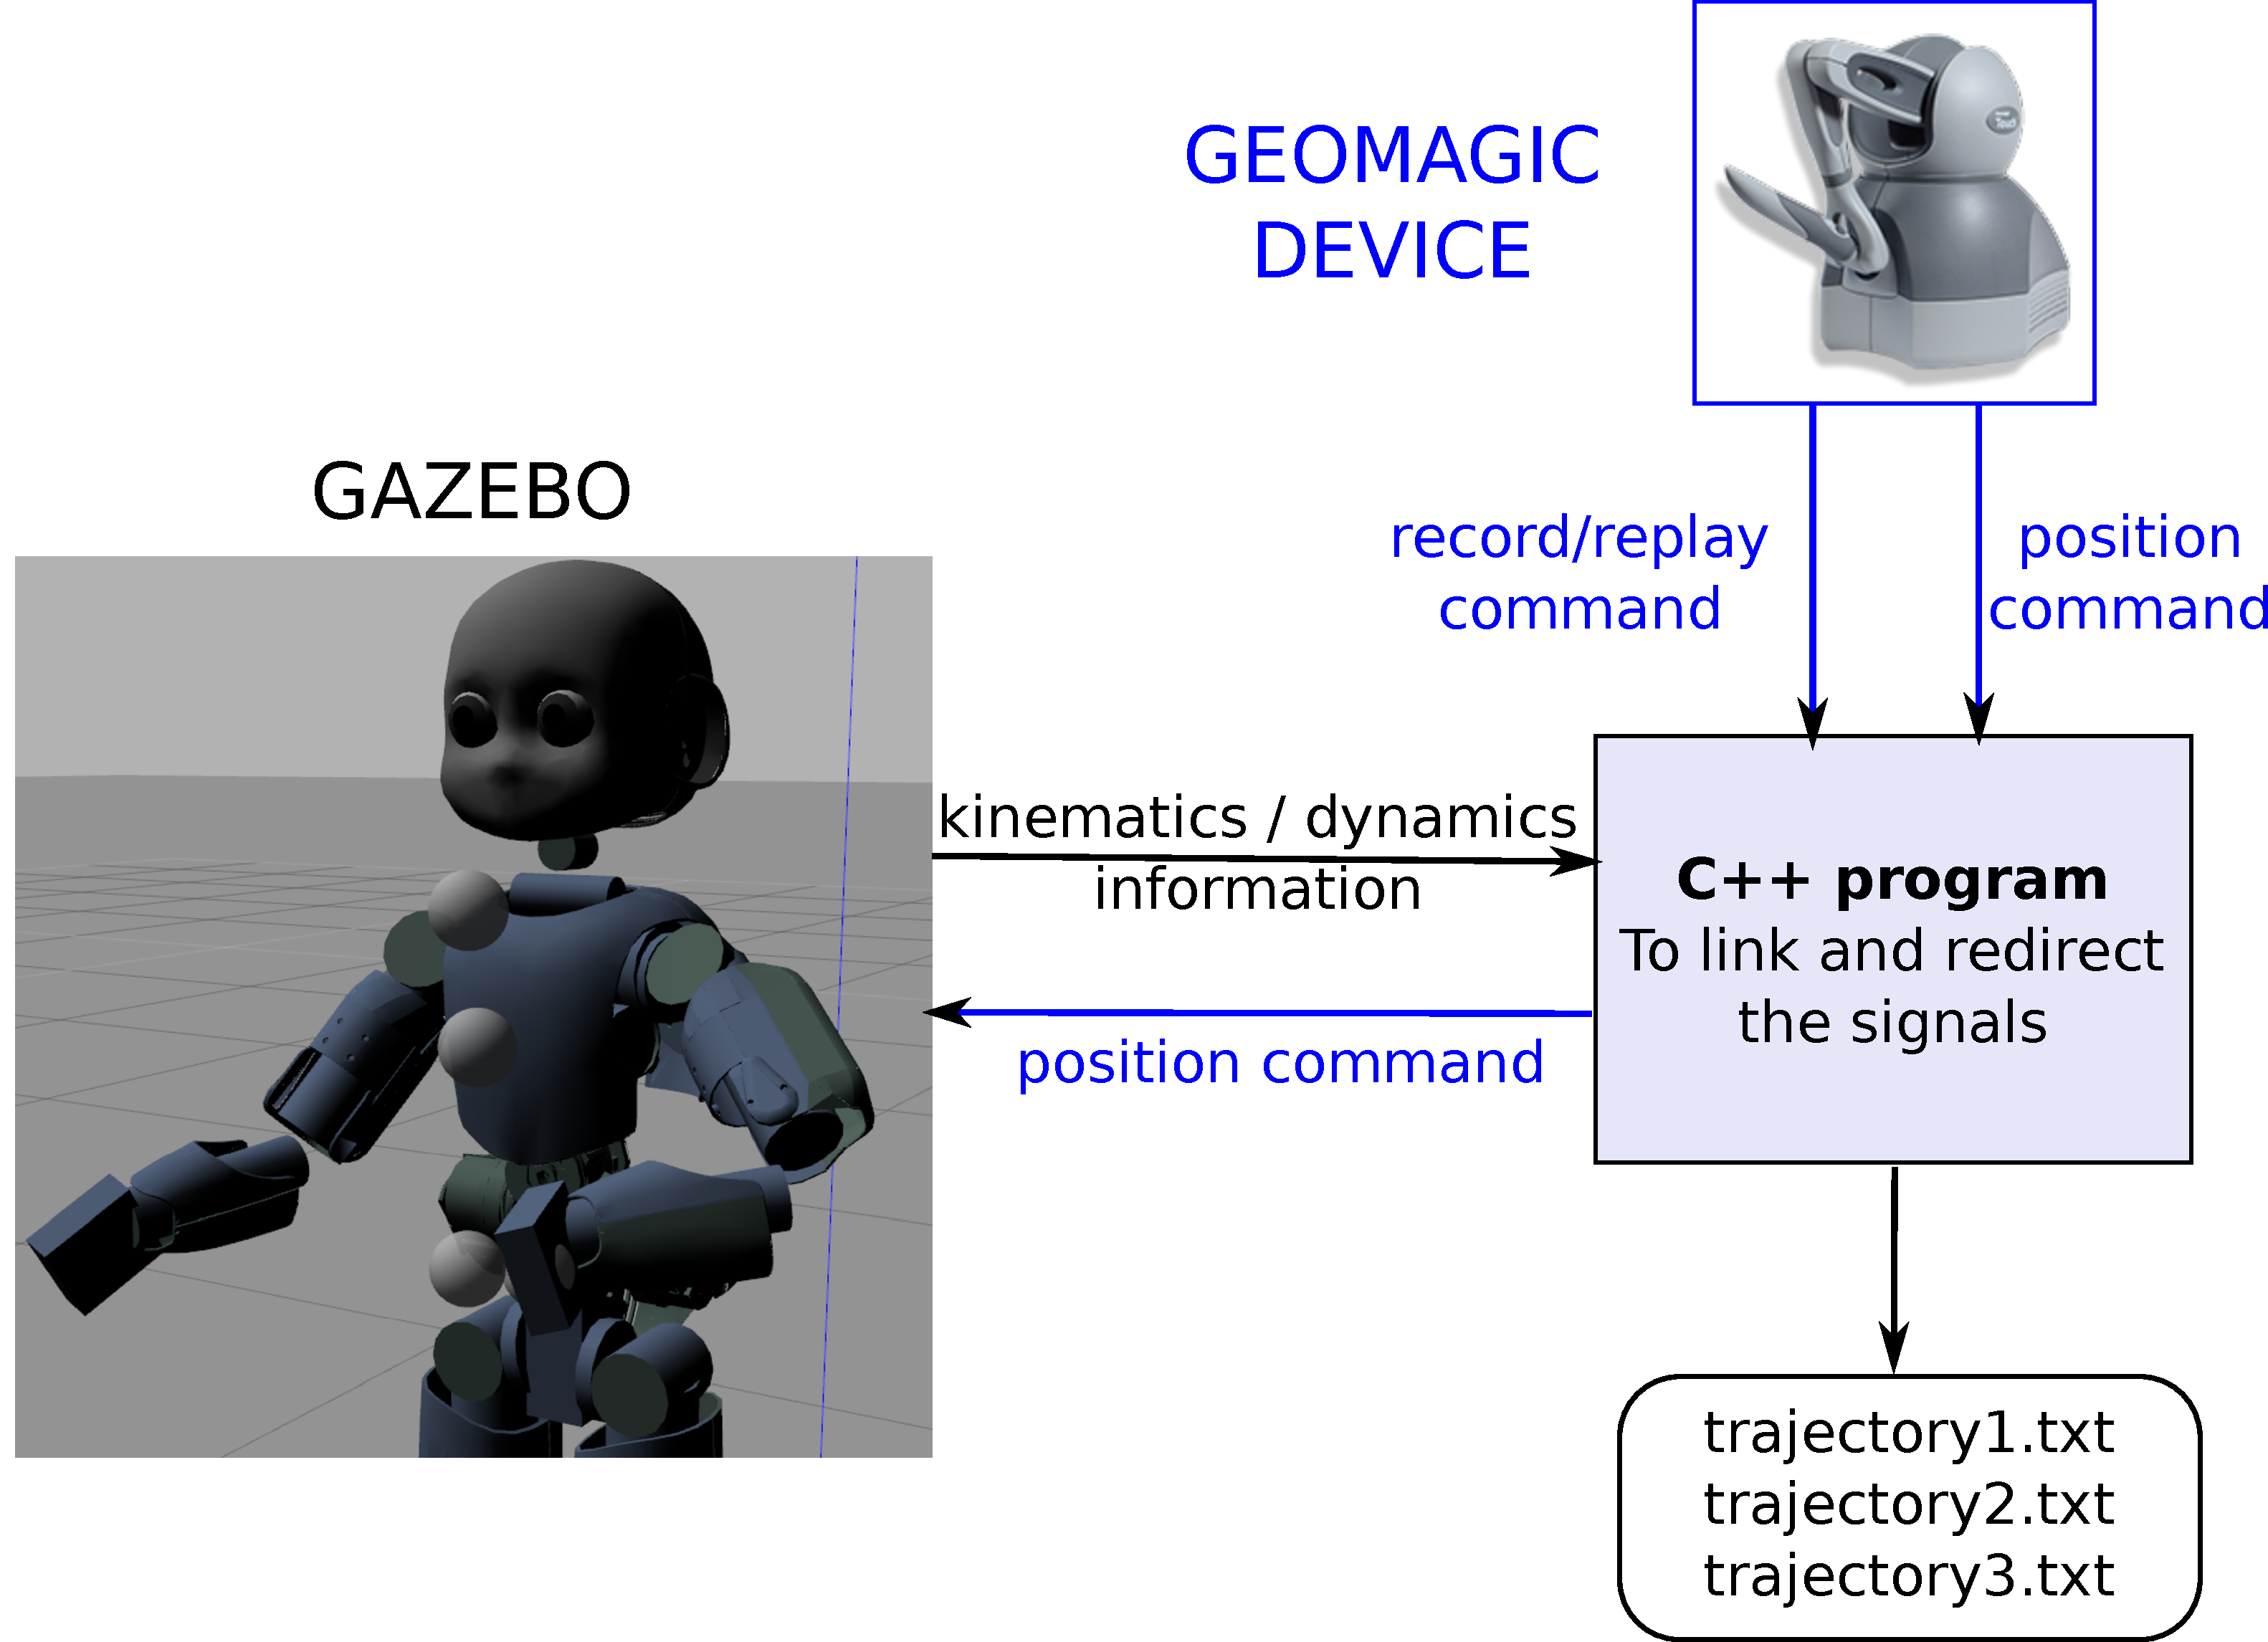
\includegraphics[width=15cm]{img/geom_ctrlV2.pdf}
%\caption{The interconnection between the Geomagic Touch and iCub in Gazebo.}
%\label{fig:systemHaptic}
%\end{figure}

\subsection{Data acquisition}
\label{sec:dataAquisition}
The dark button of the Geomagic is used to start and stop the recording of the trajectories. The operator must click and hold the button during the whole movement and release the button at the end. The trajectory is saved on a file called \textit{recordX.txt} for the $X$-th trajectory. The structure of this file is:
\begin{lstlisting}
#time #xgeo #ygeo #zgeo #fx #fy #fz #mx #my #mz #x_icub_hand #y_icub_hand #z_icub_hand
5.96046e-06 -0.0510954 -0.0127809 -0.0522504 0.284382 -0.0659538 -0.0239582 -0.0162418 -0.0290078 -0.0607215 -0.248905 -0.0872191 0.0477496$
 \end{lstlisting}
%To replay one of the trajectories from the $N$ previously recorded, the operator can click the light grey button of the Geomagic and then enter the number of the trajectory on the terminal.

%\begin{figure}[h]
%\centering
%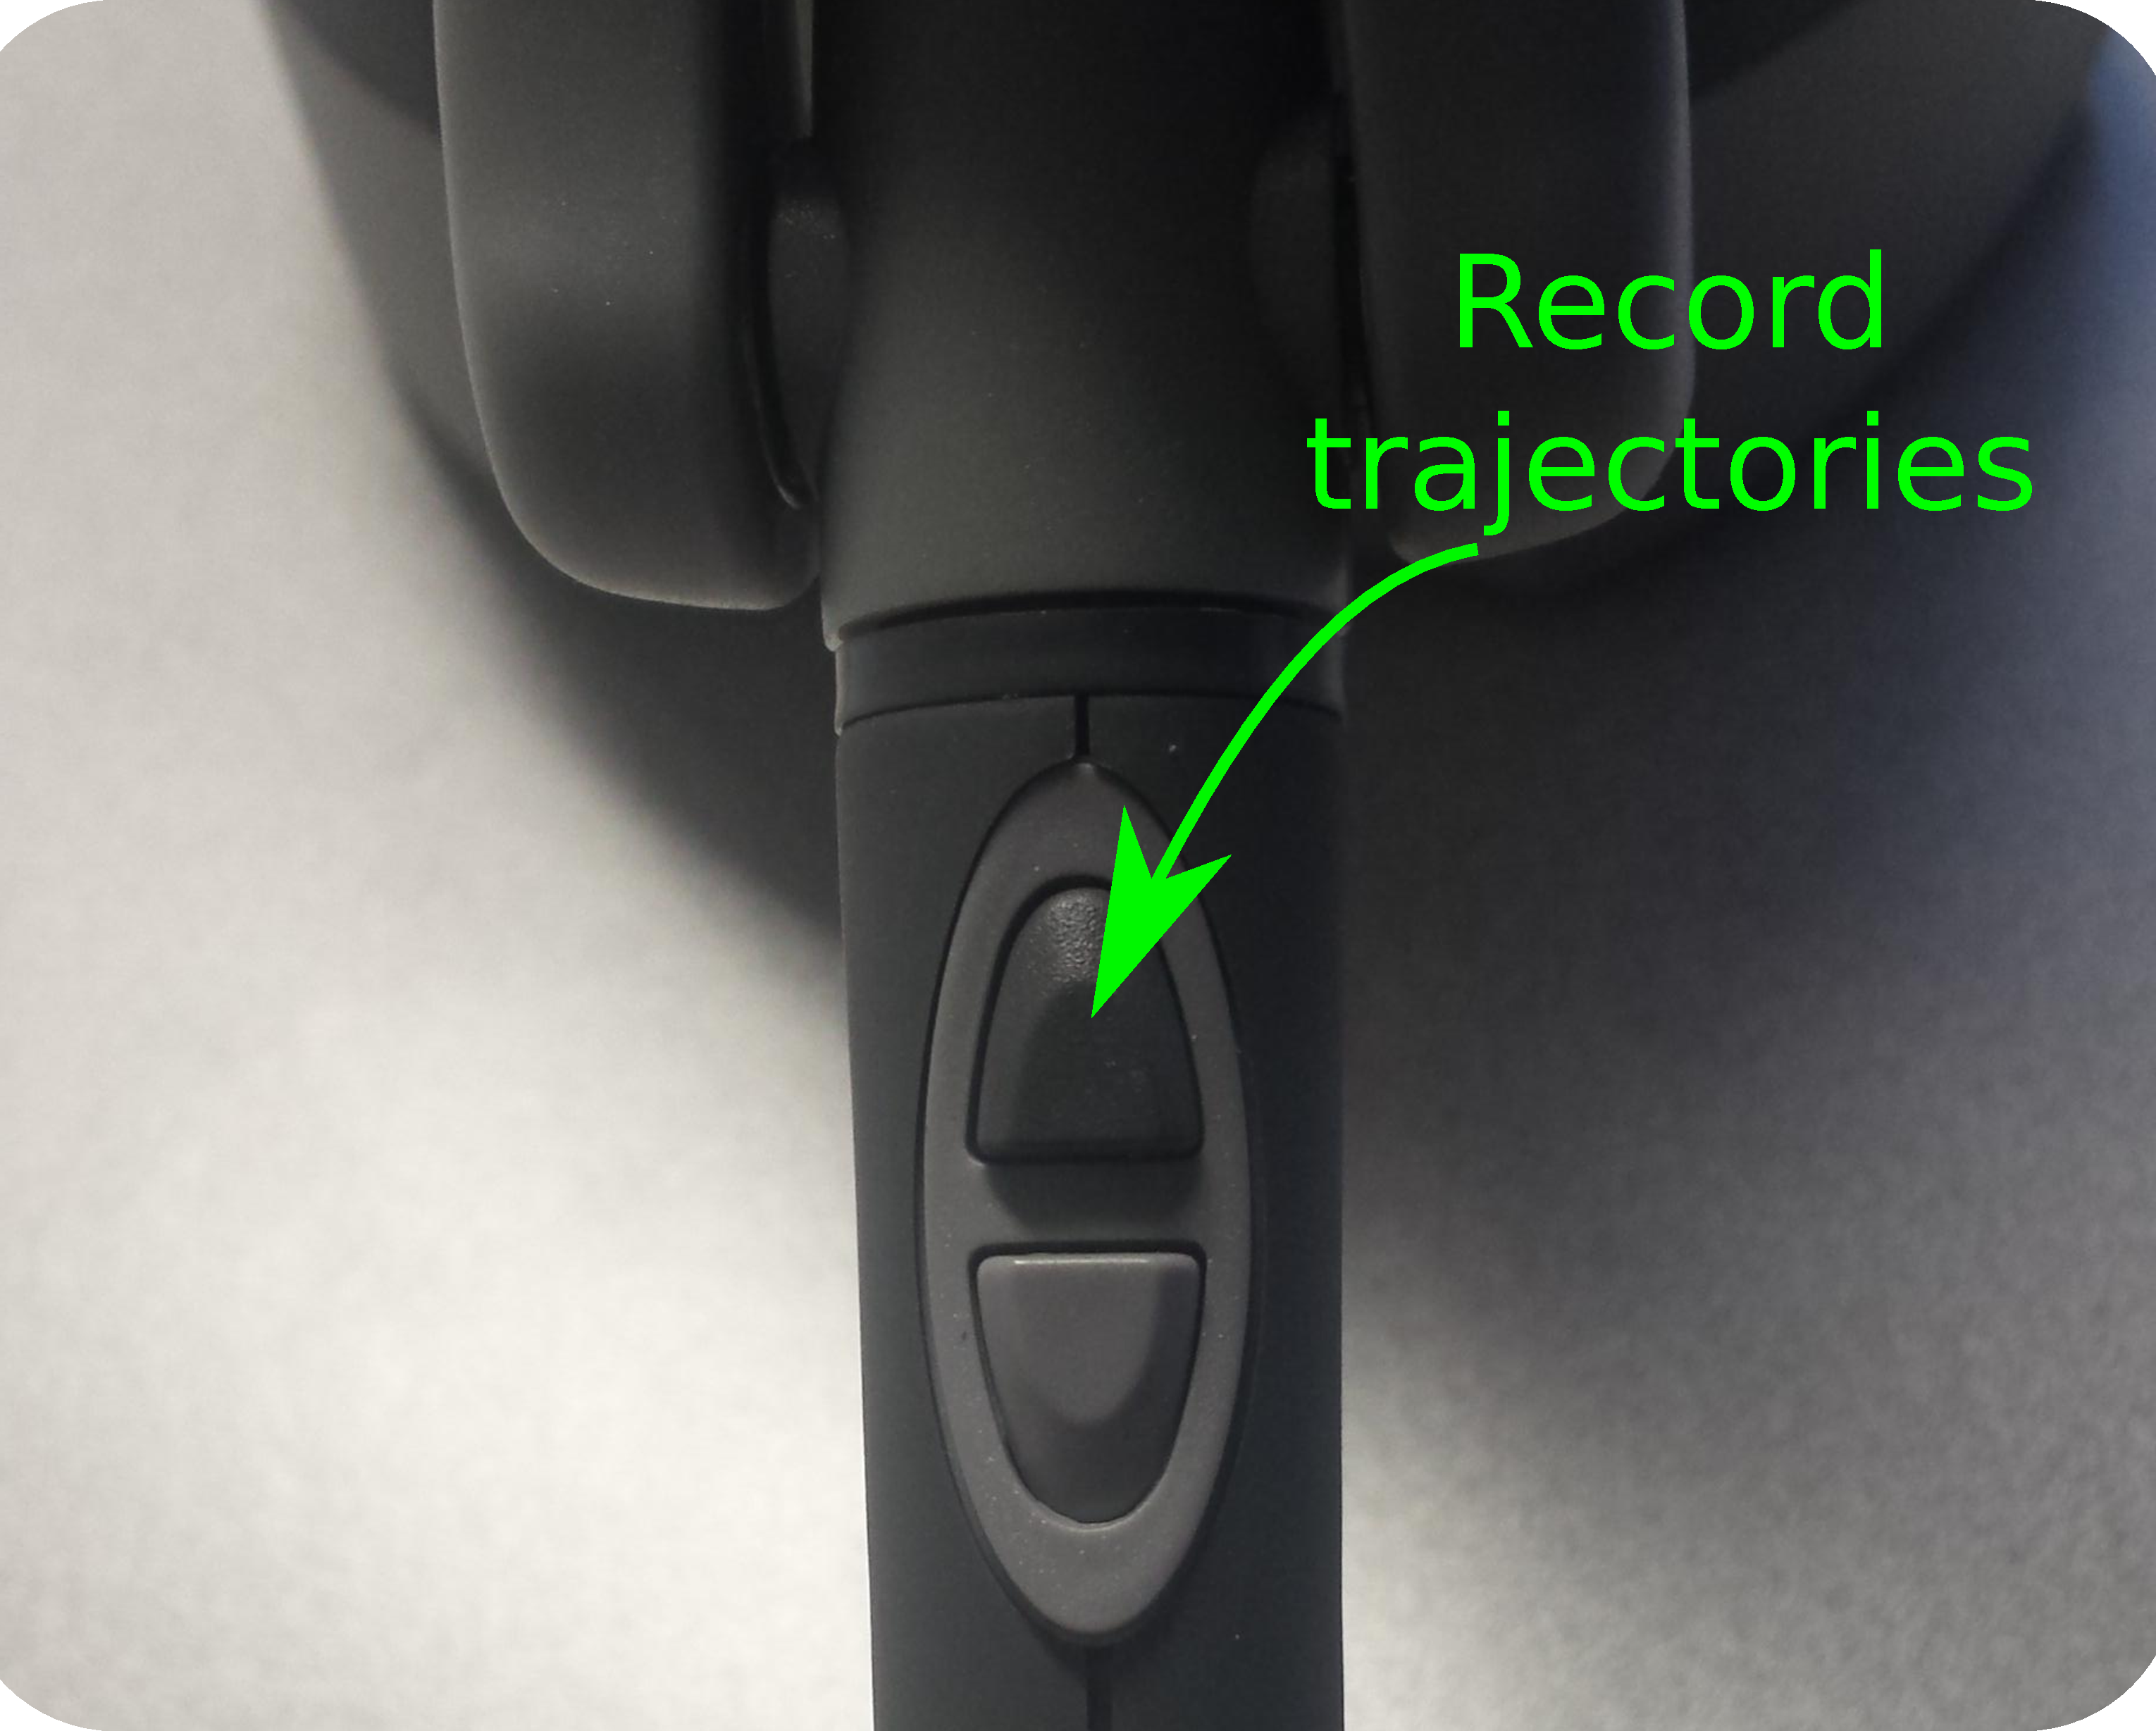
\includegraphics[height = 5cm]{img/geoButton.pdf}
%\caption{The dark button of the Geomagic.}
%\label{fig:geobuttons}
%\end{figure}

A video showing the iCub's arm moved by an user through the haptic device in Gazebo is available in Section~\ref{sec:video} (tutorial video).
The graph in Figure~\ref{fig:3TargetsTrajectories} represents some trajectories recorded with the Geomagic, corresponding to lifting the left arm of the iCub. % (in the iCub's frame).

%\begin{figure}[h]
%\centering
%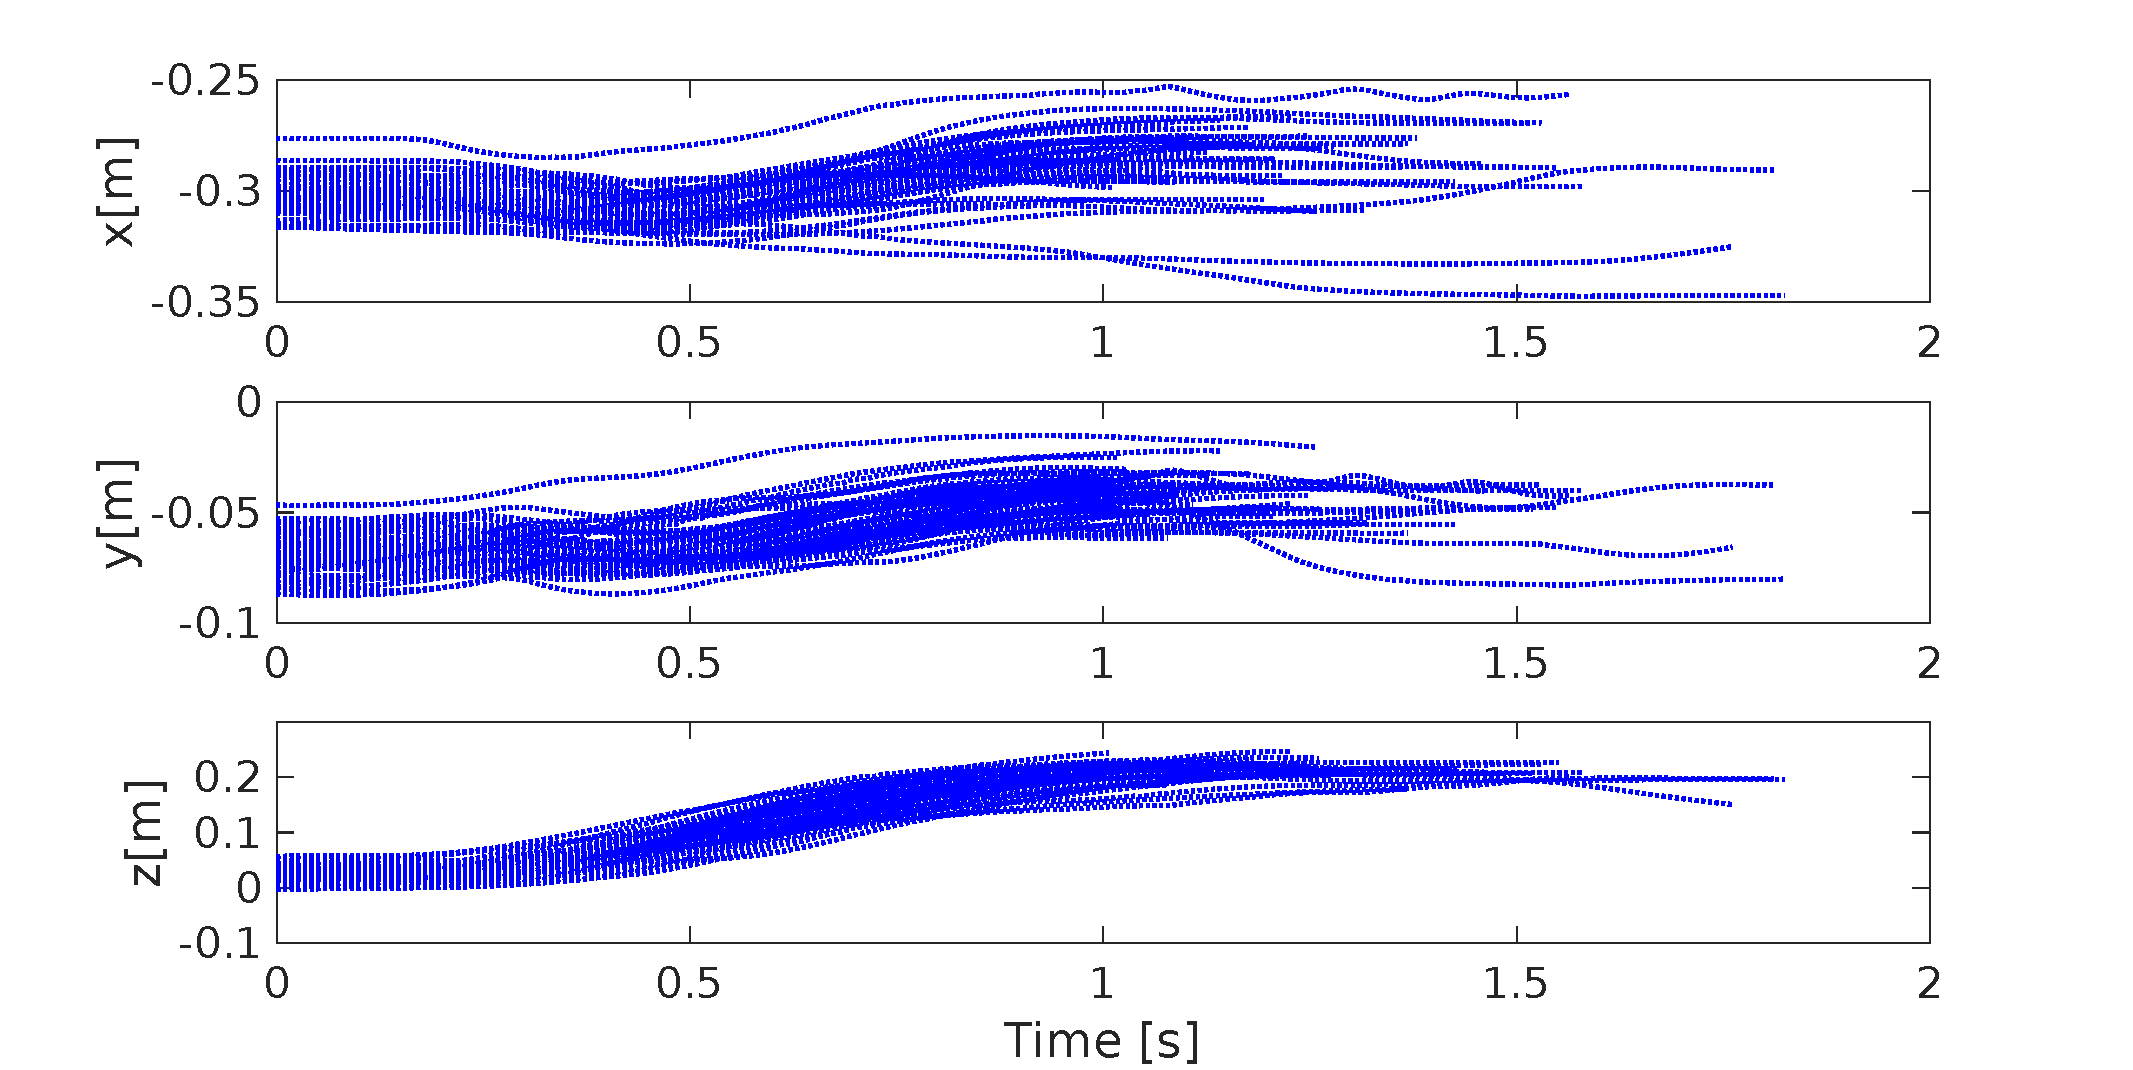
\includegraphics[width=\hsize]{img/liftingWgeomagic/trajectory_sample.pdf}
%\caption{Some trajectories recorded when the Geomagic is used to lift the left arm: Cartesian position of the end-effector.}
%\label{fig:trajectories}
%\end{figure}

Demonstrated trajectories and their corresponding forces can be recorded directly from the robot, by accessing the Cartesian interface and the \textit{wholeBodyDynamicsTree} module.\footnote{\rev{In our example, we do not use the simulated wrench information as it is very noisy. However, we provide the code and show how to retrieve it and use it, in case the readers should not have access to the real iCub.}}

In our project on Github, we provide the acquired dataset with the trajectories for the interested reader who wishes to test the code with these trajectories. Two datasets are available at \url{https://github.com/inria-larsen/icubLearningTrajectories/tree/master/MatlabProgram/Data/}:  the first dataset called ``heights" is composed of three goal-directed reaching tasks, where the targets vary in height; the second dataset called ``FLT" is composed of trajectories recorded on the real robot, whose arms moves forward, to the left and to the top.

A matlab script that learns ProMPs with such kinds of datasets is available in the toolbox, called \mcode{demo_plotProMPs.m}. It contains all the following steps.

To load the first ``heights" dataset with the three trajectories, write:
\begin{lstlisting}
t{1} = loadTrajectory('Data/heights/bottom', 'bottom', 'refNb', s_bar, 'nbInput',nbInput, 'Specific', 'FromGeom');
t{2} = loadTrajectory('Data/heights/top', 'top', 'refNb', s_bar, 'nbInput',nbInput, 'Specific', 'FromGeom');
t{3} = loadTrajectory('Data/heights/middle', 'forward', 'refNb', s_bar, 'nbInput',nbInput, 'Specific', 'FromGeom');
\end{lstlisting}

Figure \ref{fig:3TargetsTrajectories} shows the three sets of demonstrated trajectories. In the used dataset called 	``heights", we have recorded $40$ trajectories per movement primitive.

%\begin{figure}[h]
%\centering
%{
%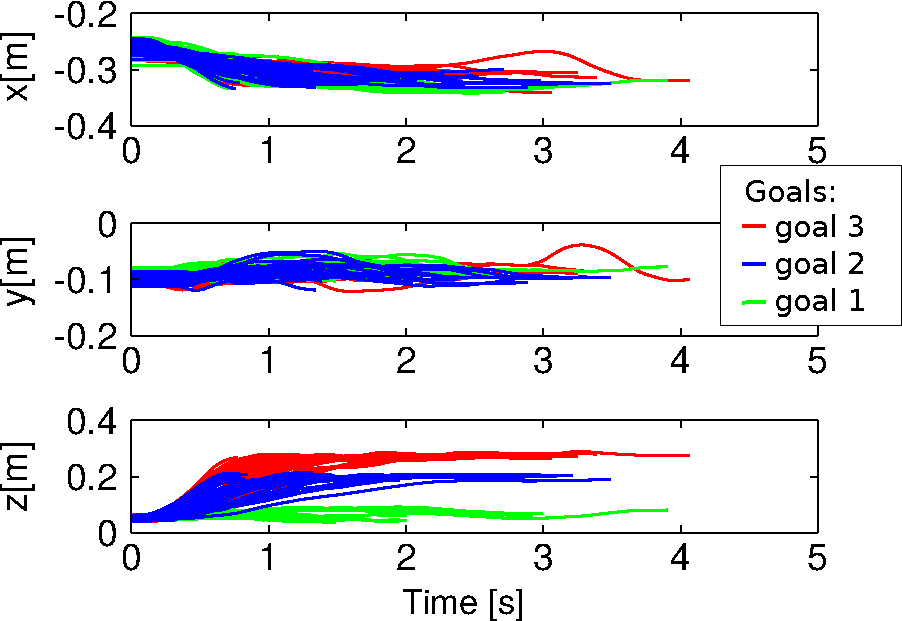
\includegraphics[width=12cm]{img/3DOFtrajectories.pdf}
%}
%\caption{Trajectories guided by the iCub's partner where he reaches three different positions that variate in height: in green the "bottom", in blue "middle" and in red "top goal positions. This plot represents only Cartesian position without force information.}% trajectories x (top),y(middle) and(bottom) without force information that are also recorded.}
%\label{fig:3TargetsTrajectories}
%\end{figure}

\subsection{Learning the ProMPs}


We need to first learn the ProMPs associated to the three observed movements. 
First, we partition the collected dataset into a training set and test dataset for the inference. One random trajectory for the inference is used:
%Before learning them, we pick from the training set one of the observed trajectory to test the inference, by writing for each $i$-th ProMP:
\begin{lstlisting}
[train{i},test{i}] = partitionTrajectory(t{i},1,percentData,s_bar);
\end{lstlisting}
The second input parameter specifies that we select only one trajectory, randomly selected, to test the ProMP. %With another number, for instance $10$, $10\%$ of the recorded data would be used for tests.

Now, we compute the three ProMPs with:

\begin{lstlisting}
promp{1} = computeDistribution(train{1}, M, s_bar,c,h);
promp{2} = computeDistribution(train{2}, M, s_bar,c,h);
promp{3} = computeDistribution(train{3}, M, s_bar,c,h)
\end{lstlisting}

We set the following parameters:
\begin{itemize}
\item \mcode{s\_bar=100}: reference number of samples, which we note in this paper as $\bar{s}$.
\item \mcode{nbInput(1) = 3; nbInput(2) = 6}: dimension of the generic vector containing the state of the trajectories. It is composed of 3D Cartesian position and 6D forces and wrench information.\footnote{Note that in our example wrenches are separated from the Cartesian position, because they are not used to recognize the index of the current ProMP during the inference.}
%\rev{dimension of the generic vector containing the state of the trajectories. It is composed of 3D Cartesian position and 6D forces and wrench information. Wrenches are separated from the Cartesian position, because they are not used to recognize the index of the current ProMP during the inference.}
\item \mcode{M(1) = 5; M(2)= 5}: number of basis functions for each \mcode{nbInput} dimension.
\item \mcode{c = 1/M;h = 1/(M*M)}: RBF parameters (see Equation~\ref{eq:RBF}).
\item \mcode{expNoise = 0.00001}: the expected data noise. We assume this noise to be very low, since this is a simulation.
\item \mcode{percentData = 40}: this variable specifies the percentage of the trajectory that the robot will be observed, before infering the end.
\end{itemize}
These parameters can be changed at the beginning of the Matlab script.


Figure \ref{fig:3TargetsZTrajectoriesProMP} shows the three ProMPs of the reaching movements towards the three targets. To highlight the most useful dimension, we only plot the $z$-axis Cartesian position. However, each dimension is plotted by the Matlab script with:
\begin{lstlisting}
drawRecoverData(t{1}, inputName, 'Specolor','b','namFig', 1);
drawRecoverData(t{1}, inputName, 'Interval', [4 7 5 8 6 9], 'Specolor','b','namFig',2);
drawRecoverData(t{2}, inputName, 'Specolor','r','namFig',1);
drawRecoverData(t{2}, inputName, 'Interval', [4 7 5 8 6 9], 'Specolor','r','namFig',2);
drawRecoverData(t{3}, inputName, 'Specolor','g','namFig',1);
drawRecoverData(t{3}, inputName, 'Interval', [4 7 5 8 6 9], 'Specolor','g','namFig',2);
\end{lstlisting}

%We used the following parameters \todo{explain params...}

%\begin{figure}[h]
%\centering
%{
%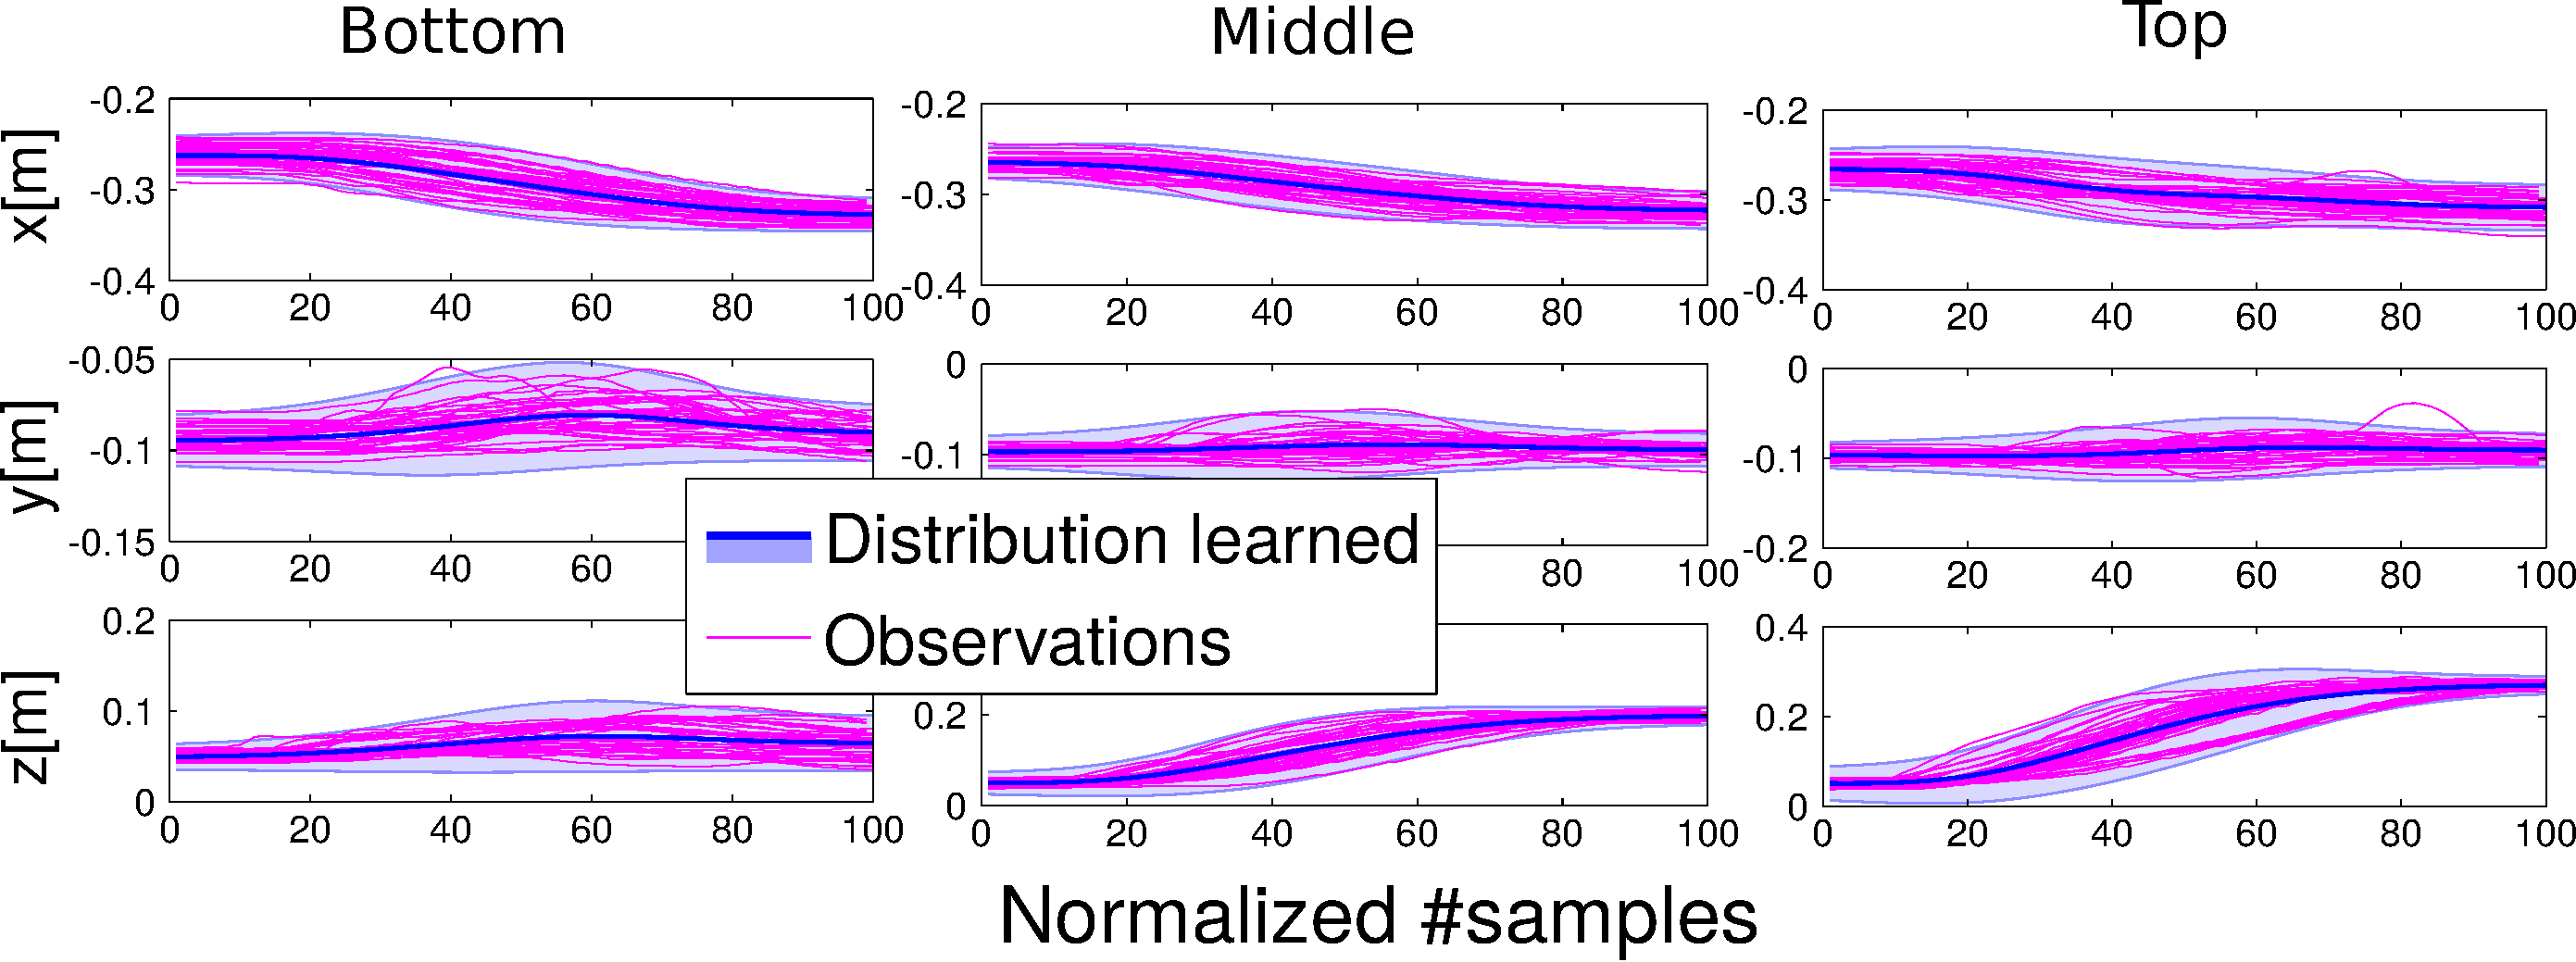
\includegraphics[width=\hsize]{img/3DOFtrajectoriesProMPsAll.pdf}\\
%}
%\caption{The ProMPs of the three different demonstrated tasks, from $39$ trajectory observations per ProMP; with M=5 basis functions per information learned; $c={1 \over M}, h={1 \over M^2}$ the parameters of the RBFs' Gaussians, $\bar{s} = 100$ the reference number of samples. Note that we represent only the Cartesian position without force information to be readable.}
%\label{fig:3TargetsTrajectoriesProMP}
%\end{figure}
\begin{figure}[h]
\centering
{
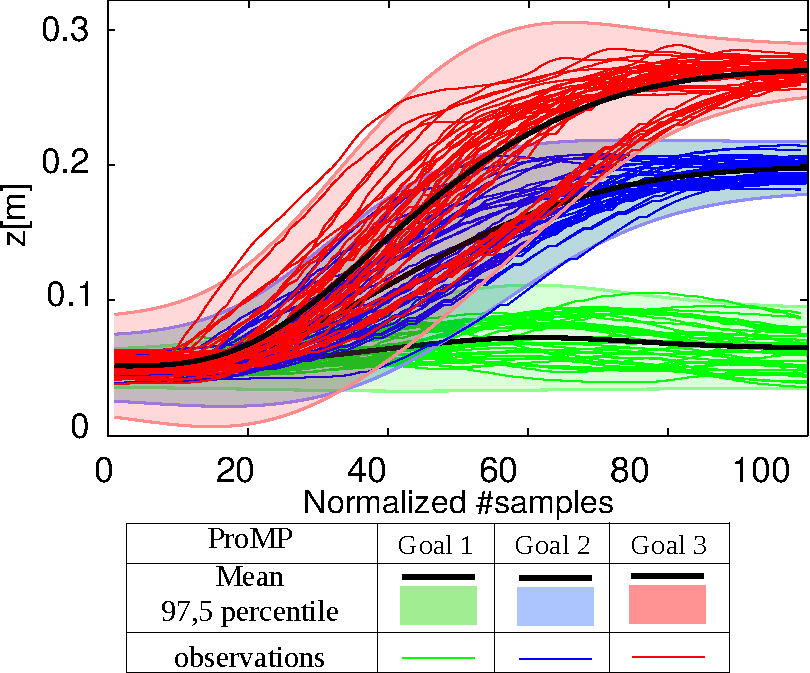
\includegraphics[height=8cm]{img/3DOFtrajectoriesProMPs.pdf}
}
\caption{The Cartesian position in the $z$-axis of the three ProMPs corresponding to reaching three targets. There are $39$ trajectory demonstrations per each ProMPm with M=5 basis functions, $c={1 \over M}, h={1 \over M^2}$ and $\bar{s} = 100$.}
\label{fig:3TargetsZTrajectoriesProMP}
\end{figure}


\subsection{Predicting the desired movement}

Now that we have learned the different ProMPs, we can predict the end of a trajectory according to the early observation $n_o$.
This number is computed from the variable \mcode{percentData} written at the beginning of the trajectory by: $n_o= |{percentData \over 100}* t_{fi}|$, where $i$ is the index of the test-trajectory

To prepare the prediction, the model the time modulation of each trajectory is computed with:
\begin{lstlisting}
    w = computeAlpha(test.nbData,t, nbInput);
    promp{1}.w_alpha= w{1};
    promp{2}.w_alpha= w{2};
    promp{3}.w_alpha= w{3};
\end{lstlisting}
This model relies on the global variation of Cartesian position during the first $n_o$ observations. The model's computations are explained in Section~\ref{sec:predictDuration}.

Now, to estimate the time modulation of the trajectory, call the function:
\begin{lstlisting}
[alphaTraj,type, x] = inferenceAlpha(promp,test{1},M,s_bar,c,h,test{1}.nbData, expNoise, 'MO');
\end{lstlisting}
Where \mcode{alphaTraj} contains the estimated time modulation $\hat{\alpha}$ and \mcode{type} gives the index of the recognized ProMP. The last parameter \mcode{x} is used for debbuging purposes.

% This variable vector contains the early observations of the trajectory translated with an offset to be centred at the mean of the recognized ProMP.  
%\marco{why the mean? Why this translation?}
%\rev{It is hard to explain in english for me, I join a picture to explain the idea}

Using this estimation of the time modulation, the end of the trajectory is inferred with:
\begin{lstlisting}
infTraj = inference(promp, test{1}, M, s_bar, c, h, test{1}.nbData, expNoise, alphaTraj);
\end{lstlisting}
%
%It can be interesting to plot the predicted trajectories for the different targets, after few or more observations. The Figure~\ref{fig:1DOFtrajectoriesPredictions3targets} represent such plots.

%\begin{figure}[!h]
%\centering
%{
%Target: green (bottom)
%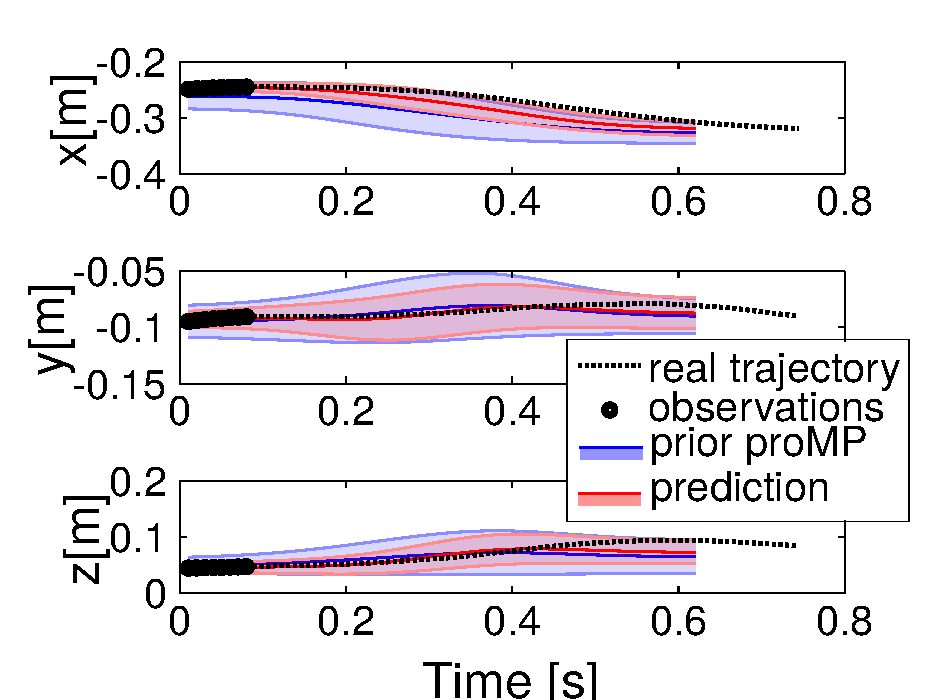
\includegraphics[width=\hsize /2]{img/infData3D/bottom10.pdf}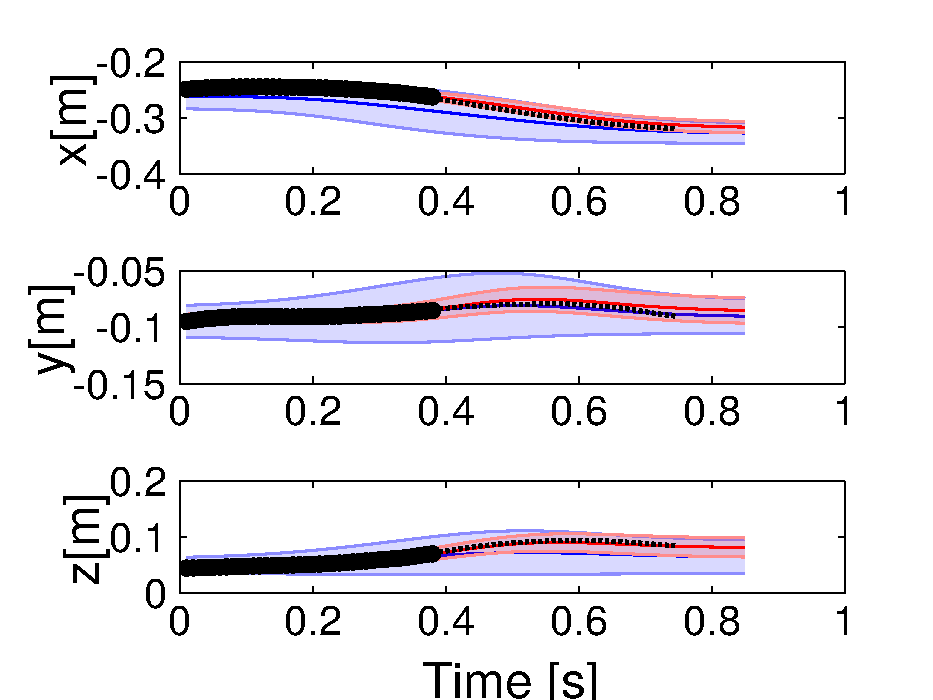
\includegraphics[width=\hsize /2]{img/infData3D/bottom50.pdf}
%%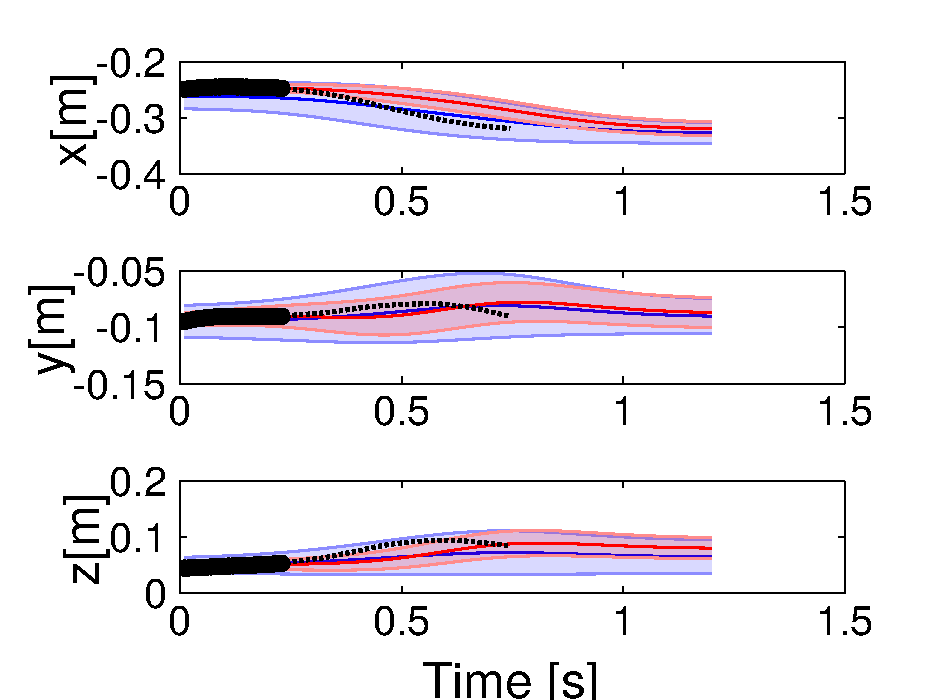
\includegraphics[width=\hsize /3]{img/infData3D/bottom30.pdf}
%Target: blue (middle)
%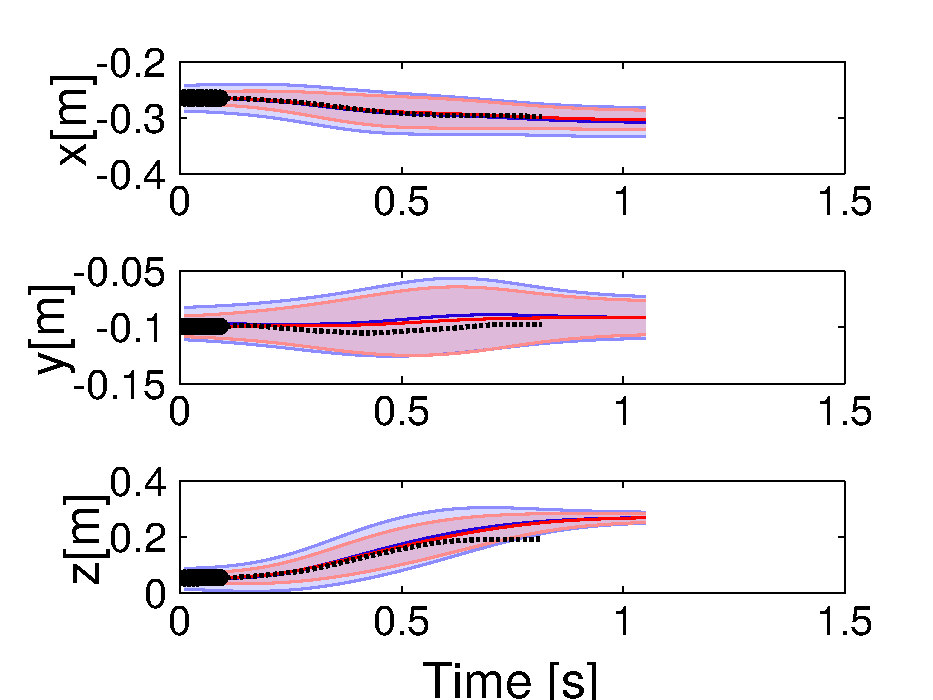
\includegraphics[width=\hsize /2]{img/infData3D/middle10Err.pdf}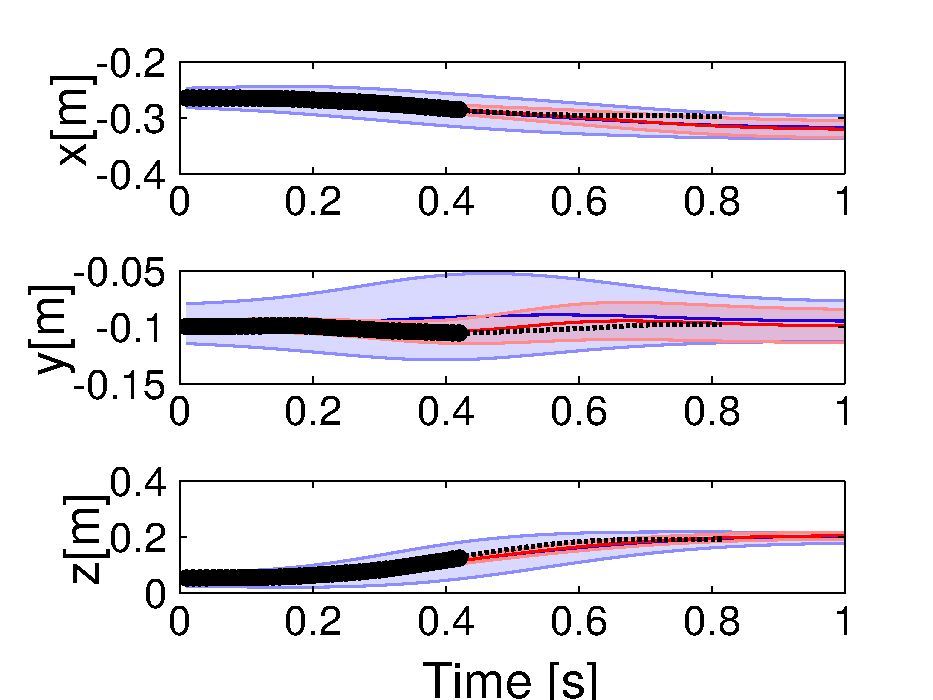
\includegraphics[width=\hsize /2]{img/infData3D/middle50.pdf}
%%%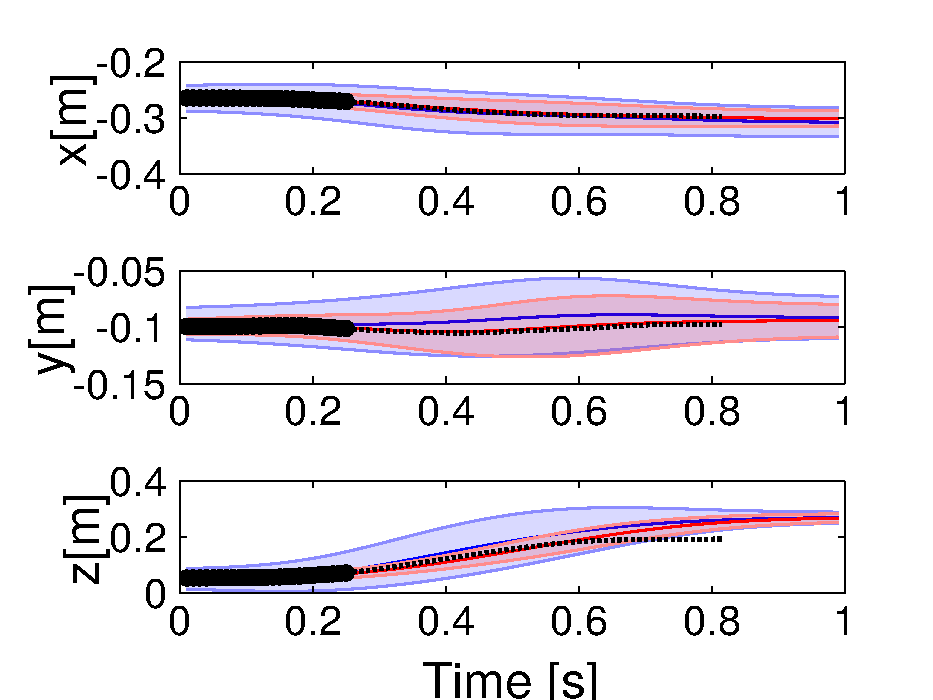
\includegraphics[width=\hsize /3]{img/infData3D/middle30Err.pdf}
%Target: red (top) 
%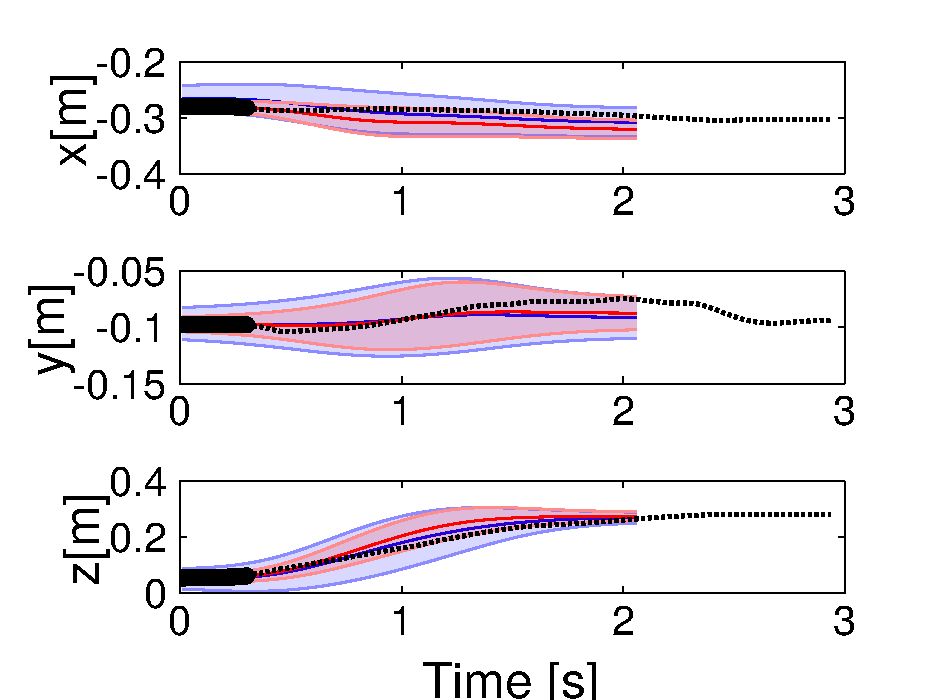
\includegraphics[width=\hsize /2]{img/infData3D/top10.pdf}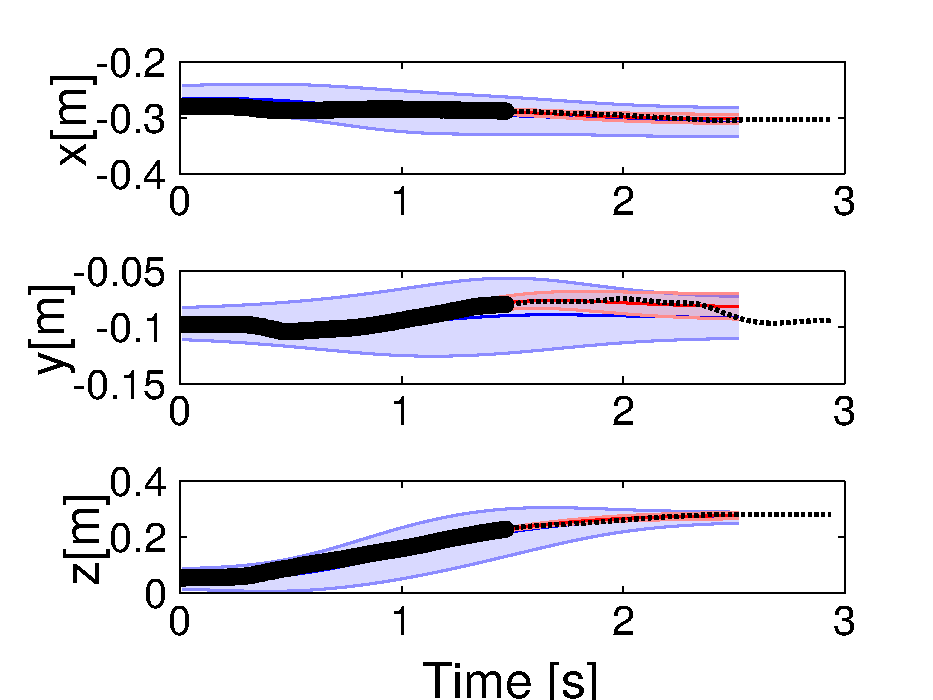
\includegraphics[width=\hsize /2]{img/infData3D/top50.pdf}
%%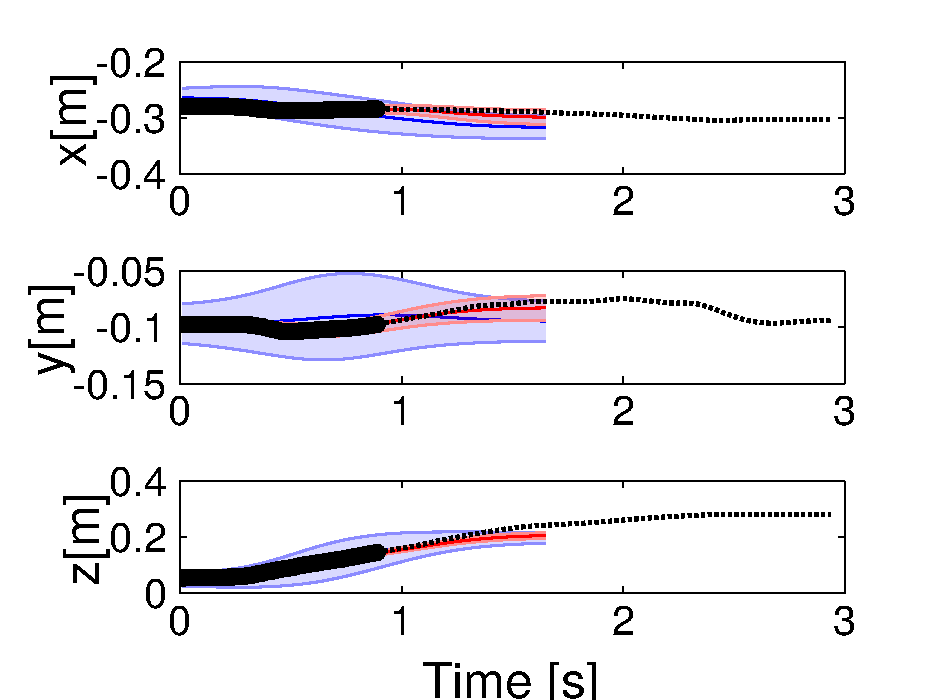
\includegraphics[width=\hsize /3]{img/infData3D/top30.pdf}
%}
%\caption{The prediction of the future trajectory thanks to the learned ProMPs computed for the  3-targets dataset (Figure \ref{fig:3TargetsZTrajectoriesProMP}) after 10 and 50 observations.}
%\label{fig:1DOFtrajectoriesPredictions3targets}
%\end{figure}

%\todo{l'image n'est pas clair, on ne voit pas grand chose : comment rendre ça plus clair ?}

As shown in the previous example, the quality of the prediction of the future trajectory depends on the accuracy of the time modulation estimation. This estimation is computed by calling the function: 
\begin{lstlisting}
%Using the model:
[alphaTraj,type, x] = inferenceAlpha(promp,test{1},M,s_bar,c,h,test{1}.nbData, expNoise, 'MO');
%Using the distance criteria:
[alphaTraj,type, x] = inferenceAlpha(promp,test{1},M,s_bar,c,h,test{1}.nbData, expNoise, 'DI');
%Using the Maximum likelihood criteria:
[alphaTraj,type, x] = inferenceAlpha(promp,test{1},M,s_bar,c,h,test{1}.nbData, expNoise, 'ML');
%Using the mean of observed temporal modulation during learning:
alphaTraj = (promp{1}.mu_alpha + promp{2}.mu_alpha + promp{3}.mu_alpha) /3.0;  
\end{lstlisting}

%% Sere: this figure seems not correct, we better remove it
%Figure \ref{fig:3DOFtrajectoriesPredictionsDuration} shows the trajectories predicted after $n_{o}=40$ observations of a desired trajectory, with or without the prediction of the trajectory duration. The last plot shows the baseline prediction, which uses the average duration extracted from the ProMP; the other plots show the prediction using (top-left) the model of the time modulation according to the global variation of position; (top-right) the maximum likelihood that the observed trajectory is assimilated to the ProMP, tested with each $\alpha$ observed during learning; the minimum distance between the observed trajectory and each ProMP rescaled with each $\alpha$ observed during the learning.
%\begin{figure}[h]
%\centering
%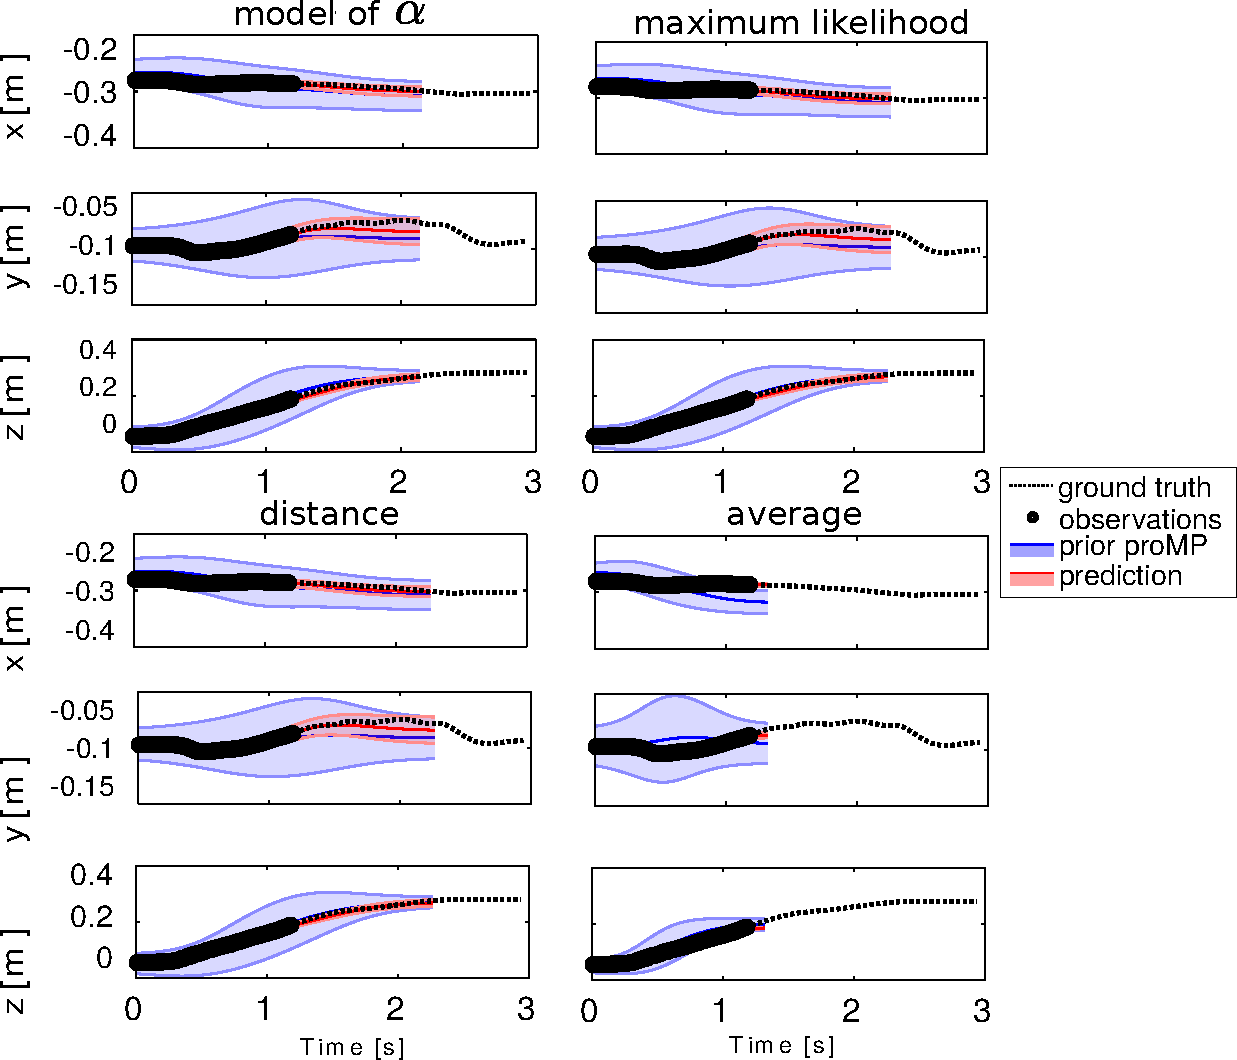
\includegraphics[height =  15cm]{img/3DOFtrajectoriesPredictionsDuration.pdf}
%\caption{The prediction of the future trajectory given $n_{o}=40$ early observations thanks to the learned ProMPs computed for the test dataset (Figure \ref{fig:3TargetsZTrajectoriesProMP}). The plots show the predicted trajectories: 1) using the model of $alpha$ according to the global position variation during the $n_o$ first observations; 2) using the maximum likelihood criteria 3) using the minimum distance criteria 4) using the average duration of the ProMP. Only one example for the red target is shown here.}
%\label{fig:3DOFtrajectoriesPredictionsDuration}
%\end{figure}

\subsection{Predicting the time modulation}\label{sec:simulatedTimeModulationModels}

In Section \ref{sec:predictDuration} we presented four main methods for estimating the time modulation parameter, discussing why this is crucial for a better estimation of the trajectory. 
Here, we compare the methods on the three goals experiment.
% consisting of learning three ProMPs where the final position varies in the height position ($z$-axis in Cartesian coordinates). 
We recorded 40 trajectories for each movement primitive, 
%executed by four different human participants, 
for a total of 120 trajectories.
%, with $40$ trajectories per each movement primitive. 
%This experiment has been done with four humans, that does ten trajectories for each movement primitive. Thus, we have forty observed trajectories per movements. 
After having computed the corresponding ProMPs, we tested the inference by providing early observations of a trajectory that the robot must finish. For that purpose, it recognizes the correct ProMP among the three precedently learned (see Section~\ref{sec:ManyProMP}) and then it estimates the time modulation parameter $\hat{\alpha}$.
%To understand how to infer a trajectory from many ProMPs, refer to Section~\ref{sec:ManyProMP}. 
Figure~\ref{fig:analyseAlpha} represents the average error of the $\hat{\alpha}$ during inference for 10 trials according to the number of observations (from 30\% to 90\% of observed data) and according to the used method. 
These methods are the ones we have just presented before that we called mean (Equation~\ref{eq:avg}), maximum likelihood (Equation~\ref{eq:ml}), minimum distance (Equation~\ref{eq:minDist}) or model (Equation~\ref{eq:model}). 
Each time, the tested trajectory is chosen randomly from the data set of observed trajectories (of course, the test trajectory does not belong to the training set, so it was not used in the learning step). 
\begin{figure}[h]
 \begin{minipage}[c]{.46\linewidth}
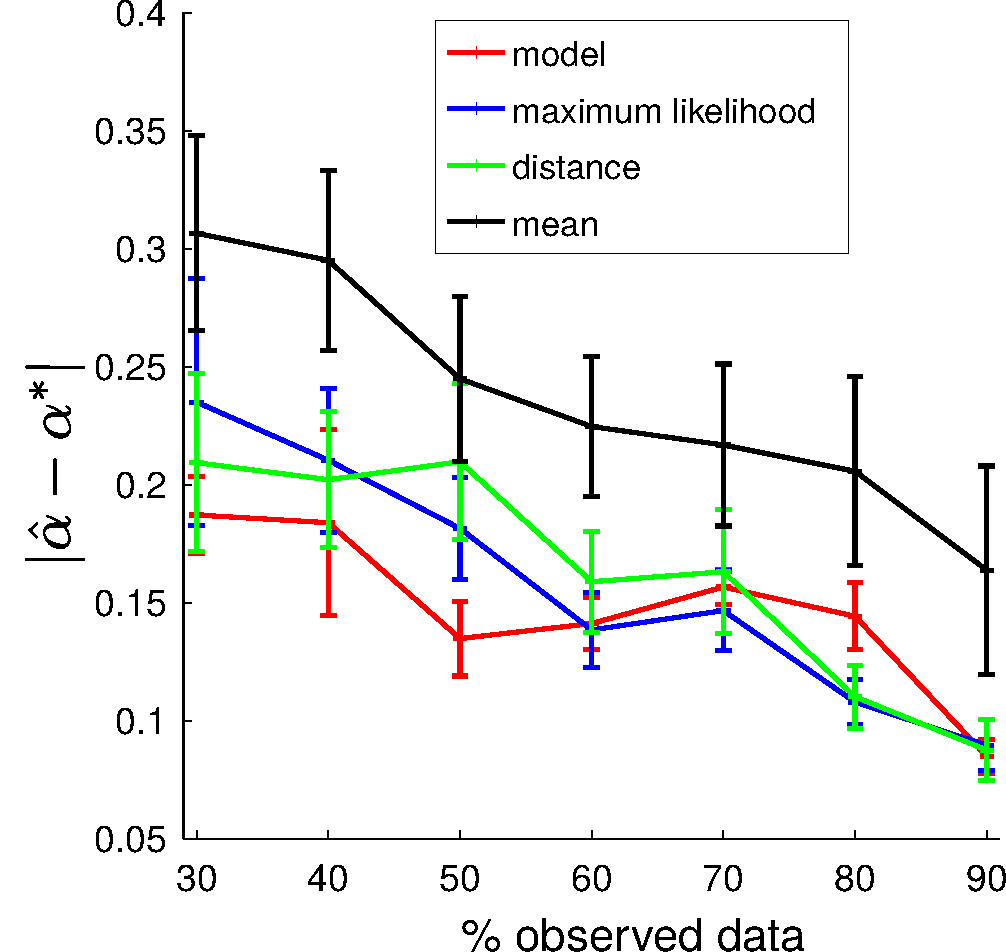
\includegraphics[width=\hsize]{img/alphaErrorAll.pdf}
\end{minipage} \hfill
   \begin{minipage}[c]{.46\linewidth}
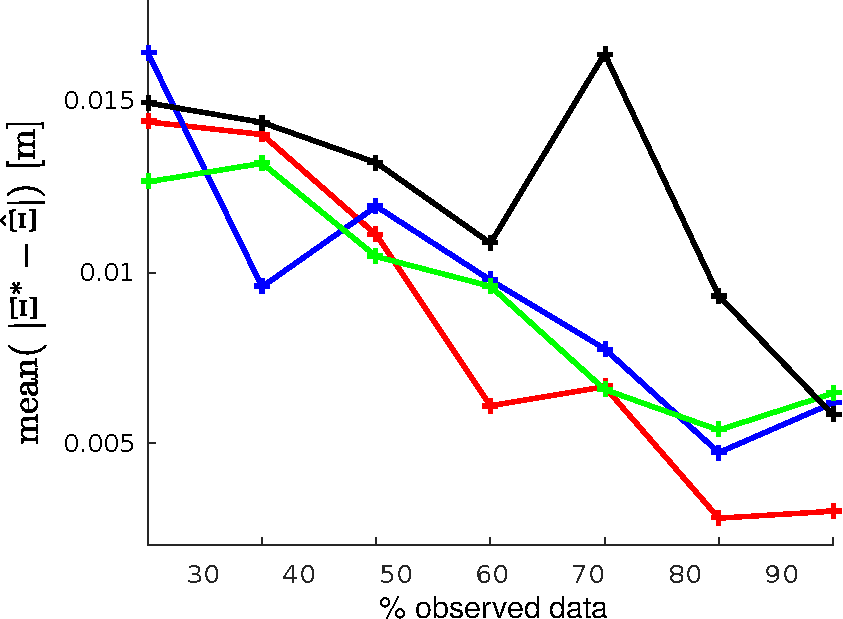
\includegraphics[width=\hsize]{img/YErrorAll.pdf}
\end{minipage}
\center
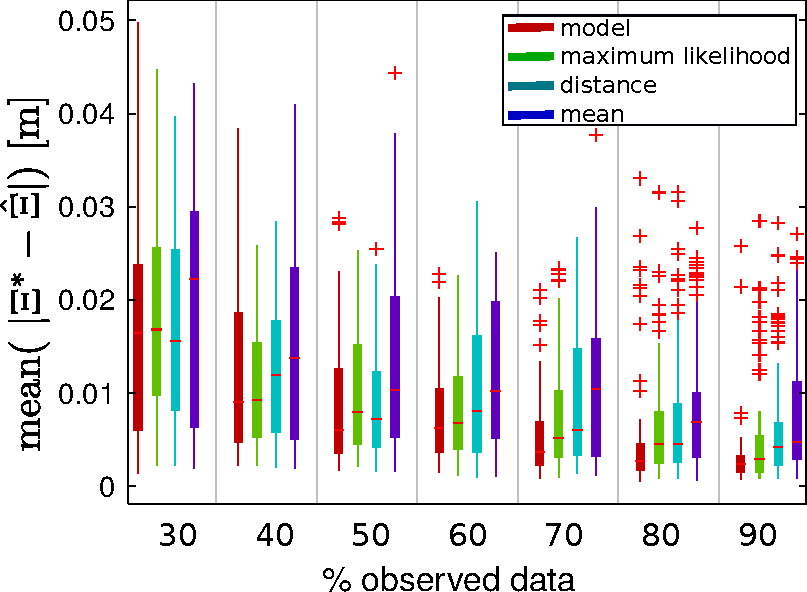
\includegraphics[height=6cm]{img/errorBoxplot.pdf}
\caption{(top left) Error of $\alpha$ estimation; (top right and bottom) error of trajectory prediction according to the number of known data and the method used. We executed 10 different trials for each case.}
\label{fig:analyseAlpha}
\end{figure}
The method that takes the average of $\alpha$ observed during learning is taken as comparison (in black). We can see that other methods are more accurate. \rev{The \textit{maximum likelihood} is increasingly more accurate, as expected. The fourth method (\textit{model}) that models the $\alpha$ according to the global variation of the trajectory's positions during the early observations is the best performing when the portion of observed trajectory is small (\textit{e.g.}, 30\%-50\%).  Since it is our interest to predict the future trajectory as early as possible, we adopted the \textit{model} method for our experiments.}
%Note that even though 



%\newpage
%%%%%%%%%%%%%%%%%%%%%%%%%%%%%%%%%%%%%%%%%%%%%%%%%%%%%%%%%%%%%%%%%%%%%%%%%%%%%%%%
\section{Application on the real iCub}
\label{sec:appliRealIcub}

\rev{In this section we present and discuss two experiments with the real robot iCub.}

\rev{In the first, we take inspiration from the experiment of the previous Section \ref{sec:3ProMPsAppli}, where the ``tasks'' are exemplified by simple point-to-point trajectories demonstrated by a human tutor. In this experiment we explore how to use wrench information and use known demonstrations as ground truth, to evaluate the quality of our prediction.}
%The task consists in collaborating with a human operator to sort objects. 

%As an example, imagine a classic object sorting scenario, where the tasks could be transferring the objects to the correct bin or tray, or an assembly scenario where the tasks are different object-picking and manipulation trajectories, to be performed with or without the human partner.
%}

\rev{In the second experiment, we set up a more realistic collaborative scenario, inspired by collaborative object sorting. 
In such applications, the robot is used to lift an object (heavy, or dangerous, or that the human cannot manipulate, as for some chemicals or food), the human inspects the object and then decides if it is accepted or rejected. Depending on this decision, the object goes on a tray or bin in front of the robot, or on a bin located on the robot side. 
Dropping the objects in two cases must be done in a different way. Realizing this application with iCub is not easy, as iCub cannot lift heavy objects and has a limited workspace. Therefore, we simplify the experiment with small objects and two bins. The human simply starts the robots movement with physical guidance, and then the robot finishes the movement on its own.
In this experiment the predicted trajectories are validated on-the-fly by the human operator.}

\rev{In a more complex collaborative scenario, tasks could be elementary tasks such as pointing, grasping, reaching, manipulating tools (the type of task here is not important, as long as it can be represented by a trajectory).}


\subsection{Three simple actions with wrench information}

\rev{Task trajectories, in this example, have both position and wrench information.
In general, it is a good idea to represent collaborative motion primitives in terms of both position and wrenches, as this representation enables using them in the context of physical interaction.
 Contrarily to the simulated experiment, here the inferred wrenches $\hat{F}_t$ correspond to the wrenches the robot should perceive if the partner was manually guiding the robot to perform the entire movement: indeed, these wrenches are computed from the demonstrations used to learn the primitive. 
The predicted wrenches can be used in different ways, depending on the application.
For example, if the partner breaks the contact with the robot, the perceived wrenches will be different. If the robot is not equipped with tactile or contact sensors, this information can be used by the robot to ``perceive'' the contact breaking and interpret it, for example, as the sign that the human wants the robot to continue the task on its own. 
Another use for the demonstrated wrenches is for detecting abnormal forces while the robot is moving: this use can have different applications, from adapting the motion to new environment to automatically detecting new demonstrations. 
Here, they are simply used to detect when the partner breaks the contact with the robot, and the latter must continue the movement on its own.
%In the current case where the partner let go of the robot, the forces will be weaker. Thus, in future work, if wrenches are stronger that the inferred forces, the robot will stop its action and follow the partner's guidance.
}

\rev{In the following, we present how to realize the experiment for predicting the user intention with the real iCub, using our software.}
%We tested our software on the real iCub. 
The robot must learn three task trajectories represented in Figure \ref{fig:realAppli}. In red, the first trajectory goes from an initial position \rev{in front of the robot} to its left (\rev{task} A). In \rev{green}, the second trajectory goes from the same initial position to the top (\rev{task C}). In \rev{blue}, the last trajectory goes from the top \rev{position to the position on the left (task B).}

\rev{To provide the demonstrations for the tasks, the human tutor used three visual targets shown on the iCub\_GUI, a basic module of the iCub code that provides a real-time synthetic and augmented view of the robot status, with arrows for the external forces and colored objects for the targets. 
One difficulty for novice users of iCub is to be able to drive the robot's arm making it perform desired complex 3D trajectories \cite{ivaldi2017towards}, but after some practice in moving the robot's arm the operator recorded all the demonstrations.
We want to highlight that having variations in the starting or ending points of the trajectories is not at all a problem, since the ProMPs are able to deal with this variability.%, contrarily to other methods for synthesizing motion primitives.
}


%One challenge of this real-world application is that the robot's arm is not easy to handle. The user need to control all the robot's degrees of freedom with one of his hands. Moreover, the user can guide the robot in different ways, so  there is variability in movements that reach the same goal.

%Despite these difficulties, we will see that 
We will see that by using the ProMPs method and by learning the end-effector Cartesian position, the robot will be able to learn distributions over trajectories, recognize when a movement belongs to one of these distributions and infer the end of the movement.


\begin{figure}[h]
\centering
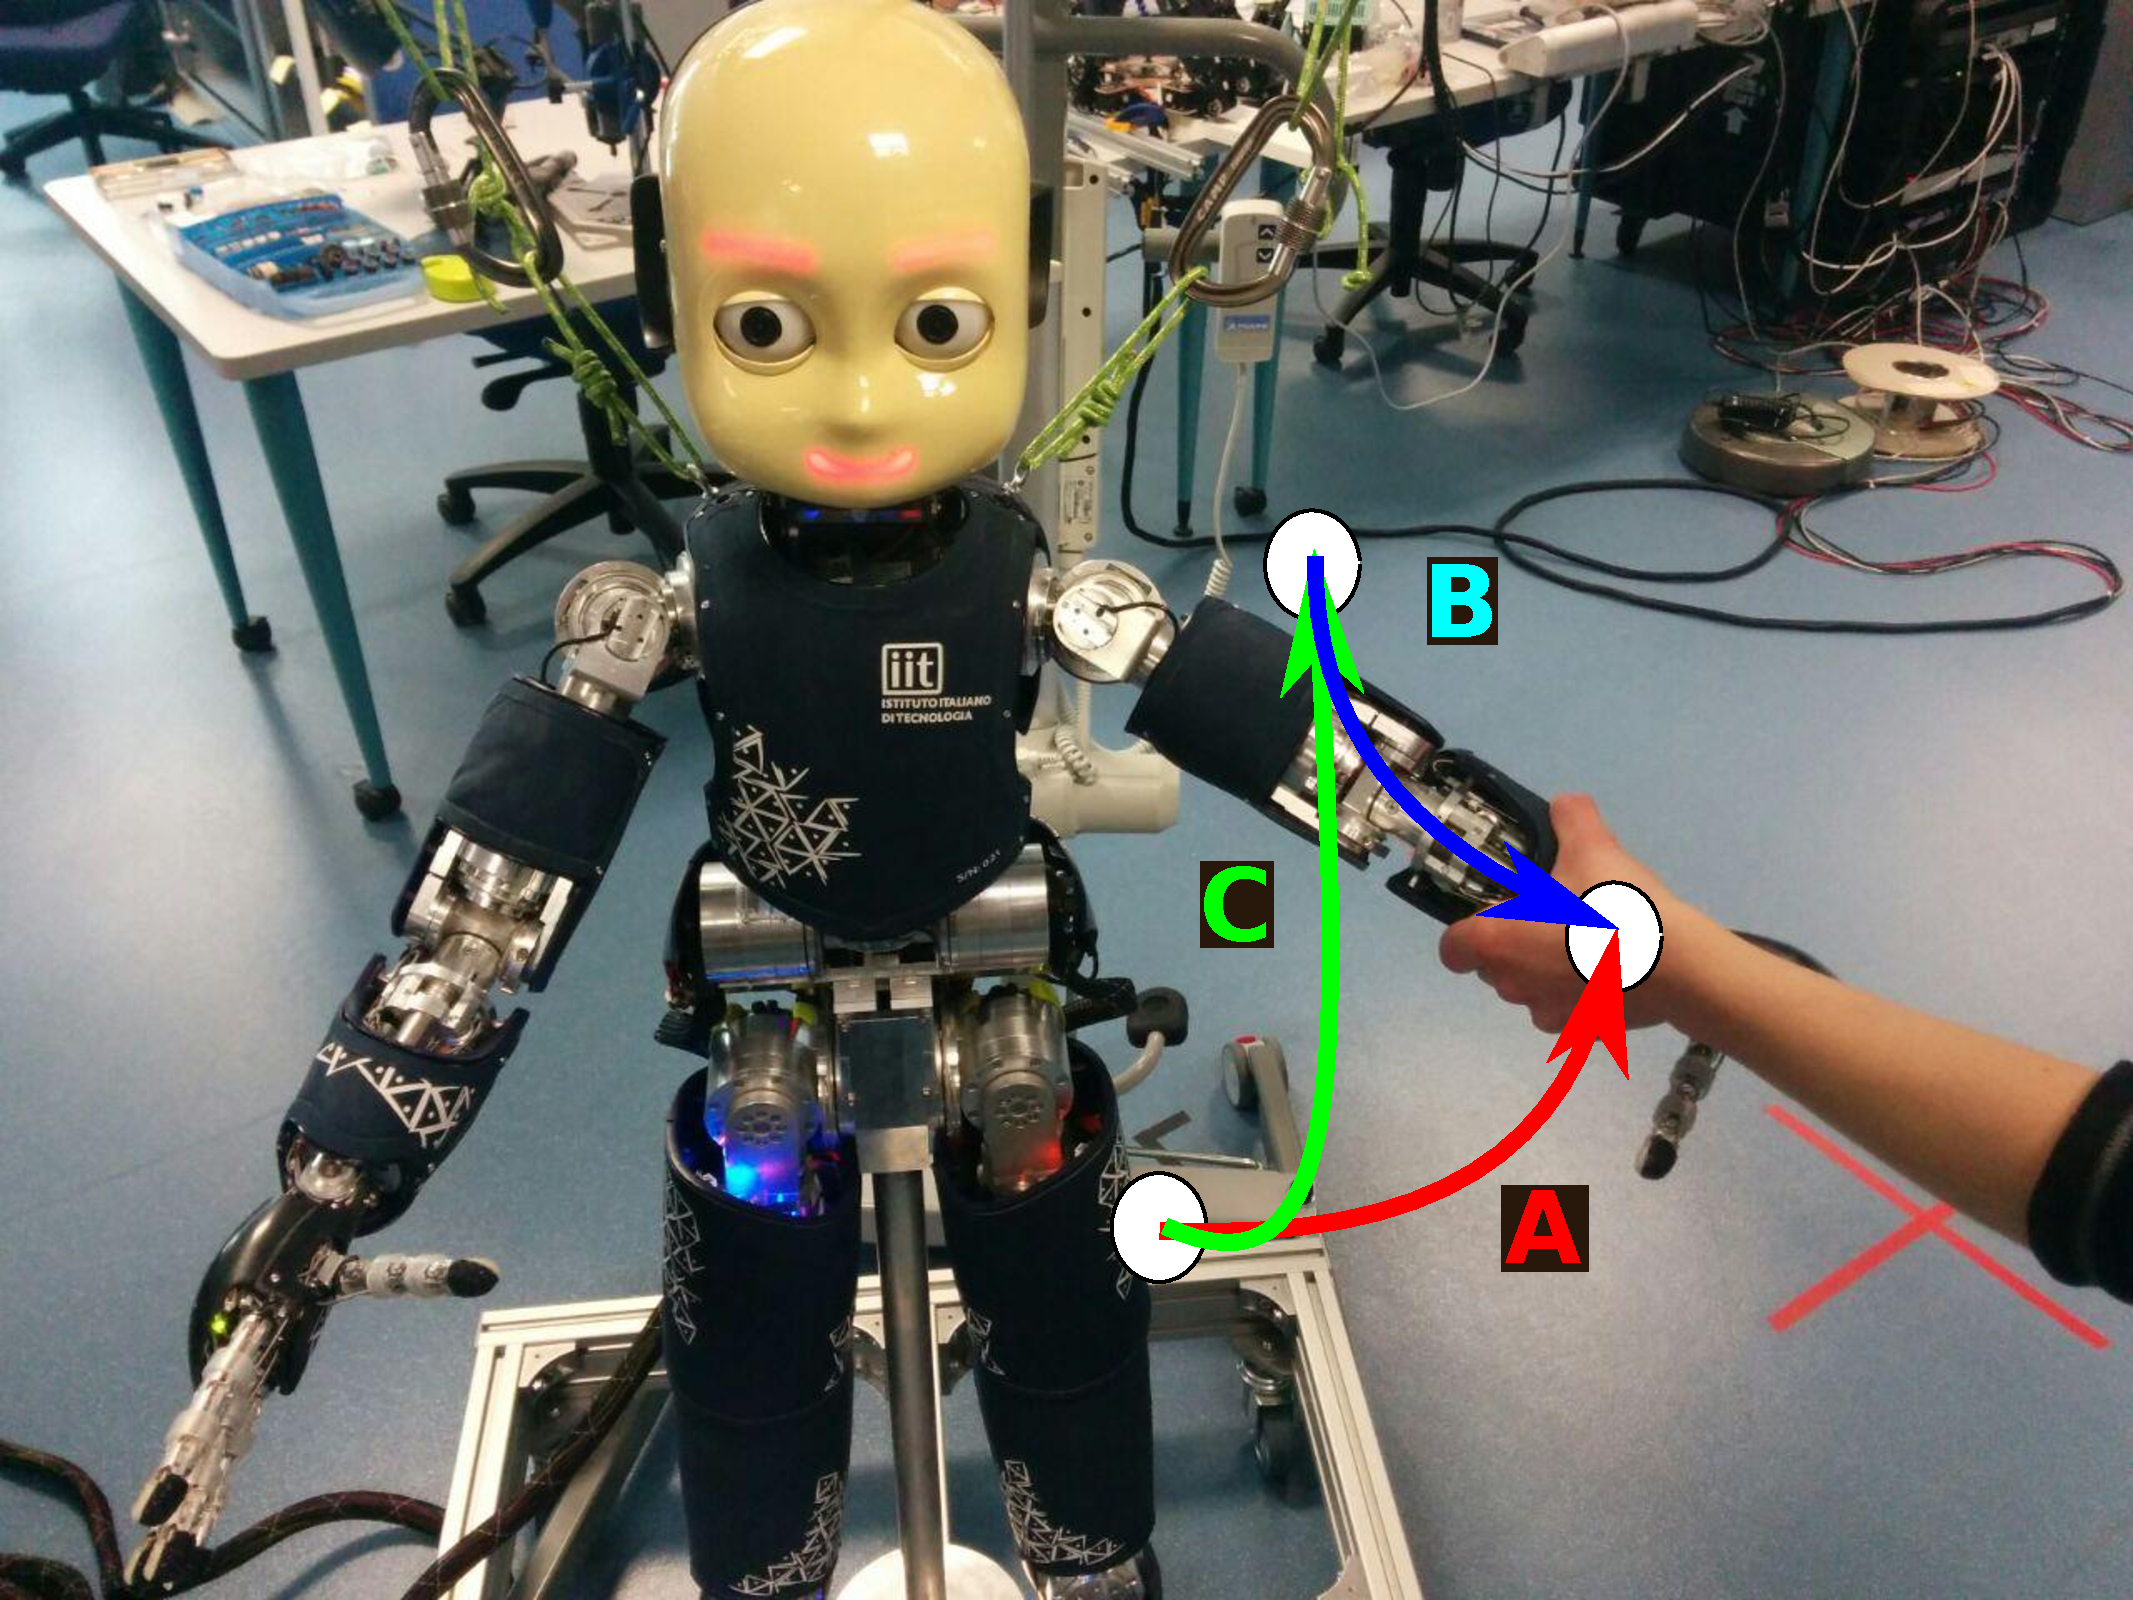
\includegraphics[width=9cm]{img/experimentRepresentation.pdf}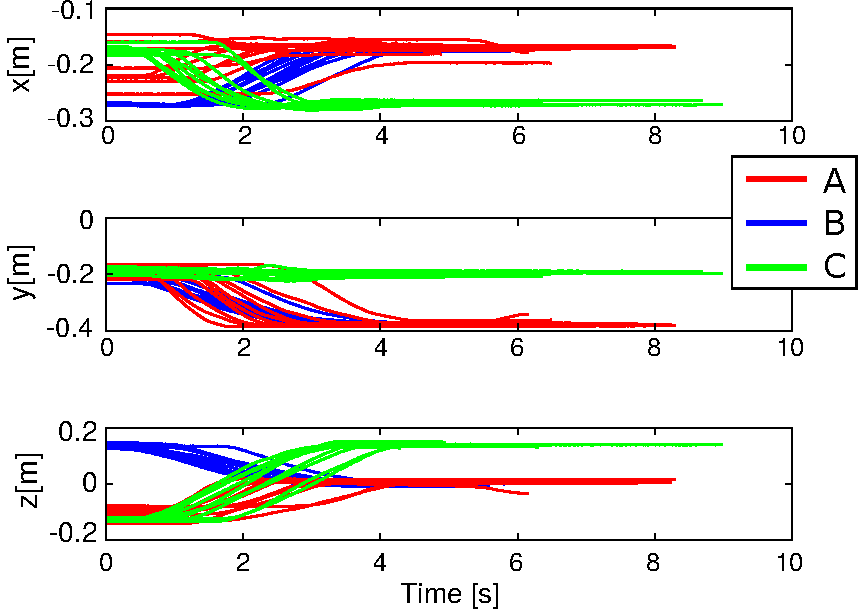
\includegraphics[width=10cm]{img/realTrajectories2.pdf}\\
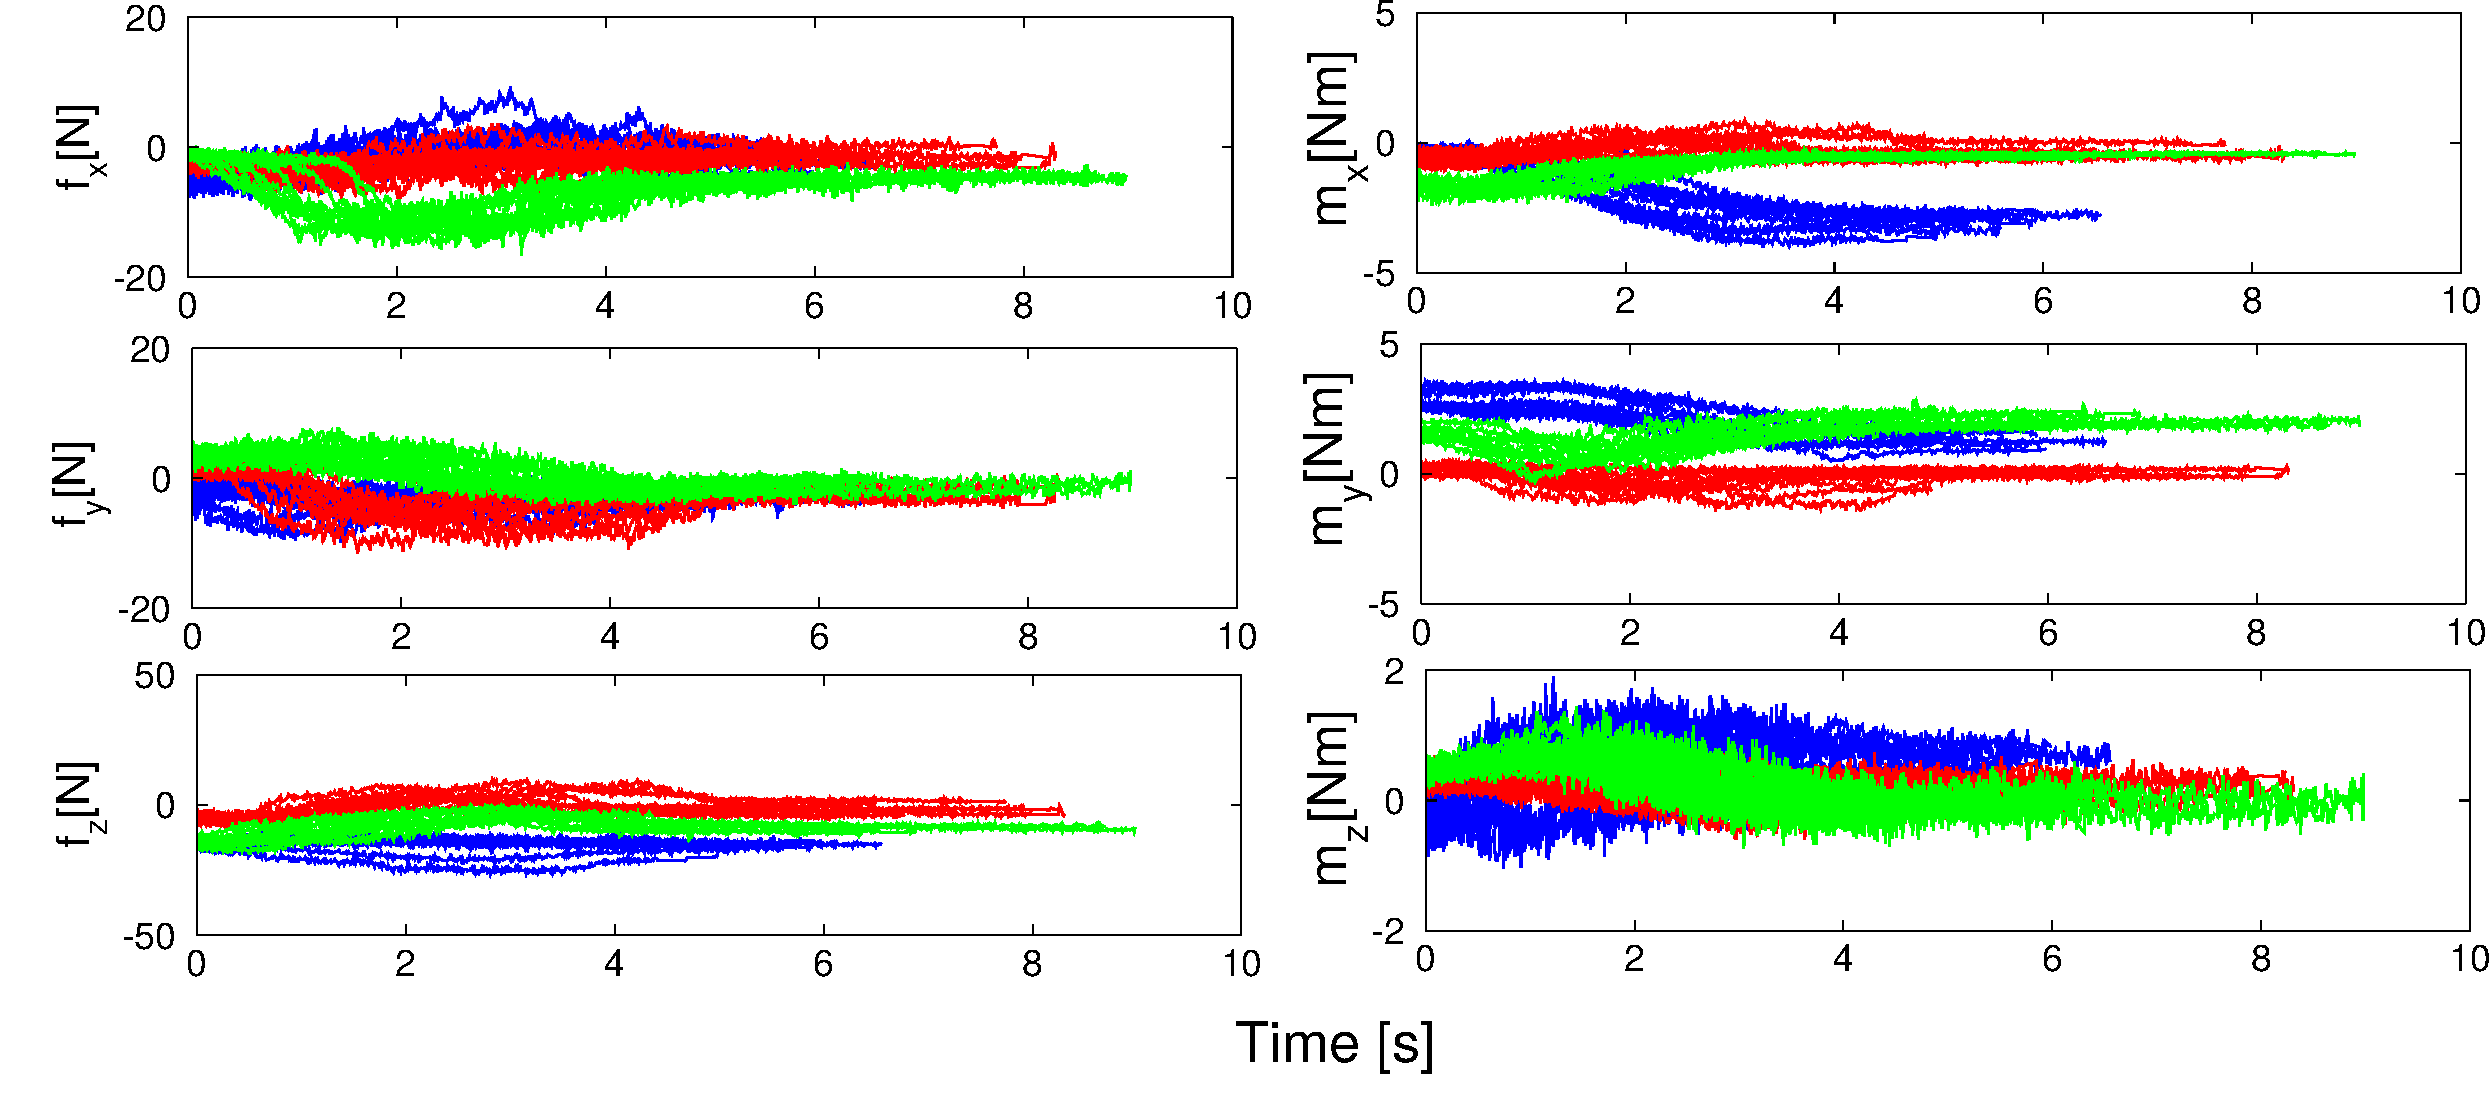
\includegraphics[width=18cm]{img/realTrajectoriesv2.pdf}
\caption{Top left: the iCub and the visualization of the three targets in its workspace, defining the three tasks A-B-C. Top right: Cartesian position information of the demonstrated trajectories for the three tasks. Bottom left and right: wrench (force and moment) information of the demonstrated trajectories.
%The three trajectories presenting the primitives A, B, and C. A color code (RGB) is used throughout the paper to facilitate the recognition of trajectories (top-left); and the corresponding test-set composed of position (top) and wrench (bottom) information.
}
\label{fig:realAppli}
\end{figure}

In this experiment, the robot received $10$ demonstrated trajectories per movement primitive, all provided by the same user. We recorded the Cartesian end-effector position and the wrenches of the robot's left arm. Data are retrieved using the function \mcode{used_functions/retrieveRealDataWithoutOrientation.m}. The output parameters of this function are three objects (one per ProMP) that contain all the required information to learn the ProMPs. 
%%From these objects, the robot learned:
%Each trajectory is:
%$$\Xi_t = \begin{bmatrix}
%[x_t & y_t & z_t ]^\top \\ [F_x & F_y & F_z]^\top \\ [m_x & m_y & m_z]^\top
%\end{bmatrix}$$
%\marco{[Obs.: What did the robot learn? The parameters $\omega$ and the distributions or the trajectories?]}
%\rev{I don't understand your question: by learning the $\omega$ parameter and the distributions, the robot learns the trajectory, isn't it?} 

In this function, the wrench information are filtered using a Matlab function called \mcode{envelope.m}\footnote{Information about this function can be found here: \url{https://fr.mathworks.com/help/signal/ref/envelope.html?requestedDomain=www.mathworks.com}}: for each trajectory \mcode{traj} and its subMatrix $M = F([1:t])$:
\begin{lstlisting}
[envHigh, envLow] = envelope(traj.M);
traj.M = (envHigh+envLow)/2;
\end{lstlisting}
These three objects are saved in \mcode{'Data/realIcub.mat'}. A Matlab script called \mcode{demo_plotProMPsIcub.m} recovers these data, using the function \mcode{load('Data/realIcub.mat')}. This script follows the same organization as the ones we previously explained in Sections~\ref{sec:example1DOF} and \ref{sec:3ProMPsAppli}. 
By launching this script, the recovered data are plotted first.

%\begin{figure}[h]
%\centering
%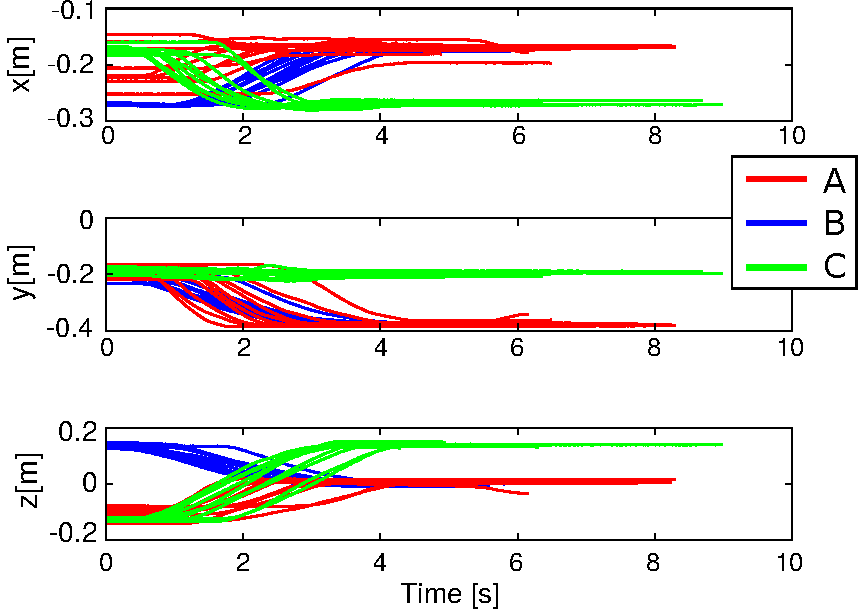
\includegraphics[height = 10cm]{img/realTrajectories2.pdf} 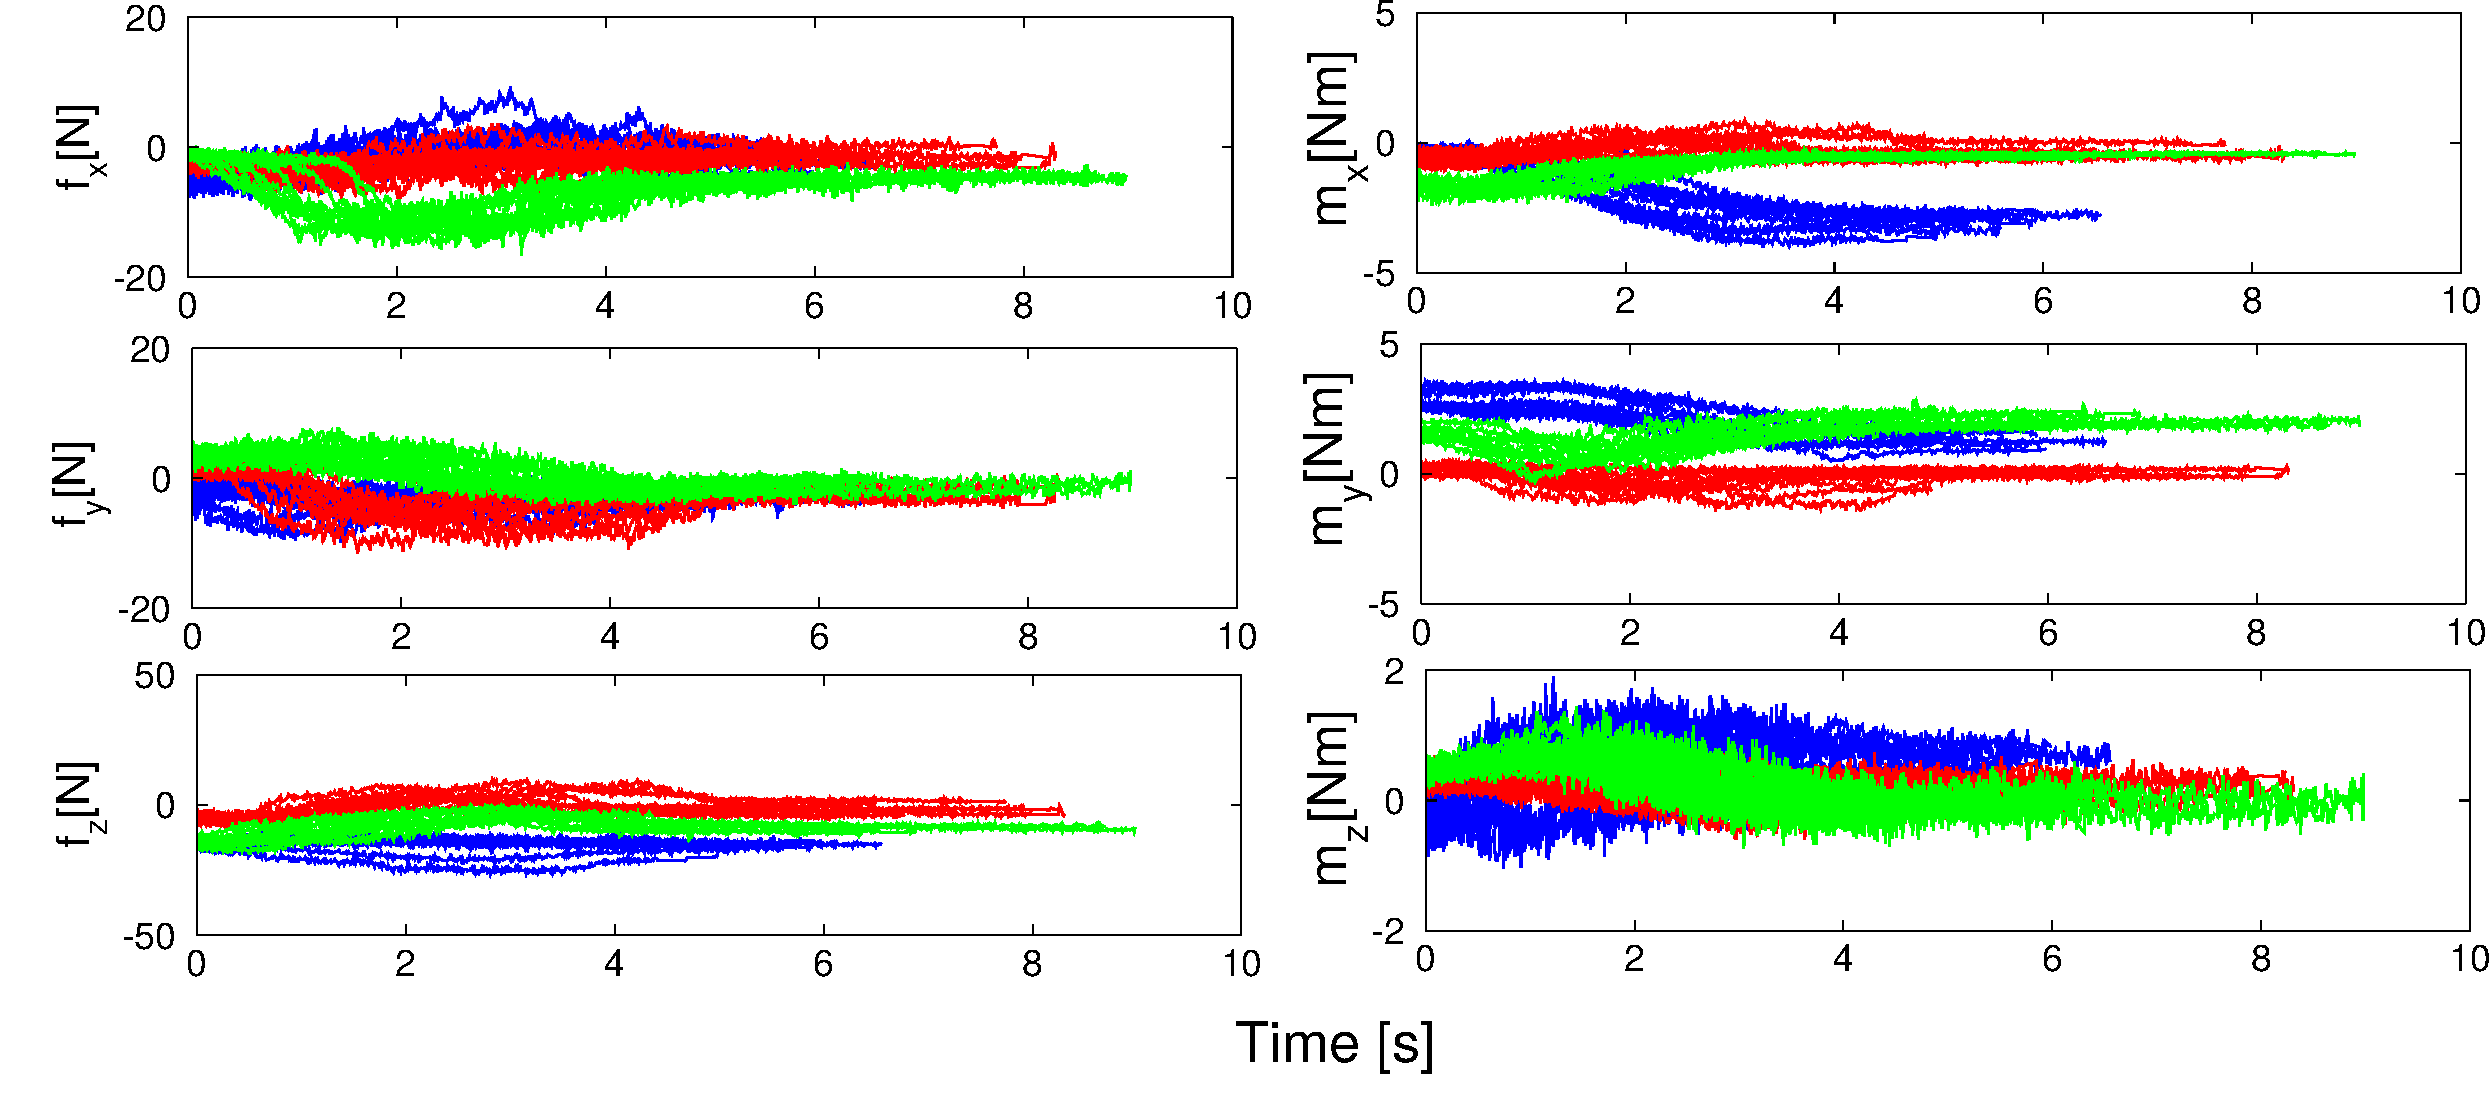
\includegraphics[width=\hsize]{img/realTrajectoriesv2.pdf} 
%\caption{Reprensentation of the three trajectories learned by the real iCub. Top: 3D Cartesian position; bottom: wrenches with 3D forces (left) and 3D moments (right).}
%\label{fig:realTraj}
%\end{figure}

Then, the ProMPs are computed and plotted, as presented in Figure~\ref{fig:realDistribution}.
In this figure, the distributions are visibly overlaid:
\begin{itemize}
\item during the whole trajectories duration for the wrench information;
% $f_x$, $f_y$, $f_z$ and $m_z$ dimensions; 
\item during the $40\%$ first samples of the trajectories for the Cartesian position information.
%$x$, $y$ and $z$ dimensions. 
\end{itemize}


%We make the hypothesis that force information is not useful for identifying trajectories. However, the robot learned it to know what are the forces' amplitude it is supposed to measure.




After this learning step, the user chooses which ProMP to test.
Using a variable that represents the percentage of observed data to be used for the inference, the script computes the number of early observations $n_o$\footnote{$n_o$ is not the same for each trajectory test, because it depends on the total duration of the trajectory to be inferred. } that will be measured by the robot. Using this number, the robot models the time modulation parameter $\alpha$\footnote{Since the model uses the $n_o$ parameter, its computation cannot be performed before this step.} of each ProMP, as explained in Section~\ref{sec:predictDuration}. 
Using this model, the time modulation of the test trajectory is estimated and the corresponding ProMP is identified.

%\begin{figure}[h]
%\centering
%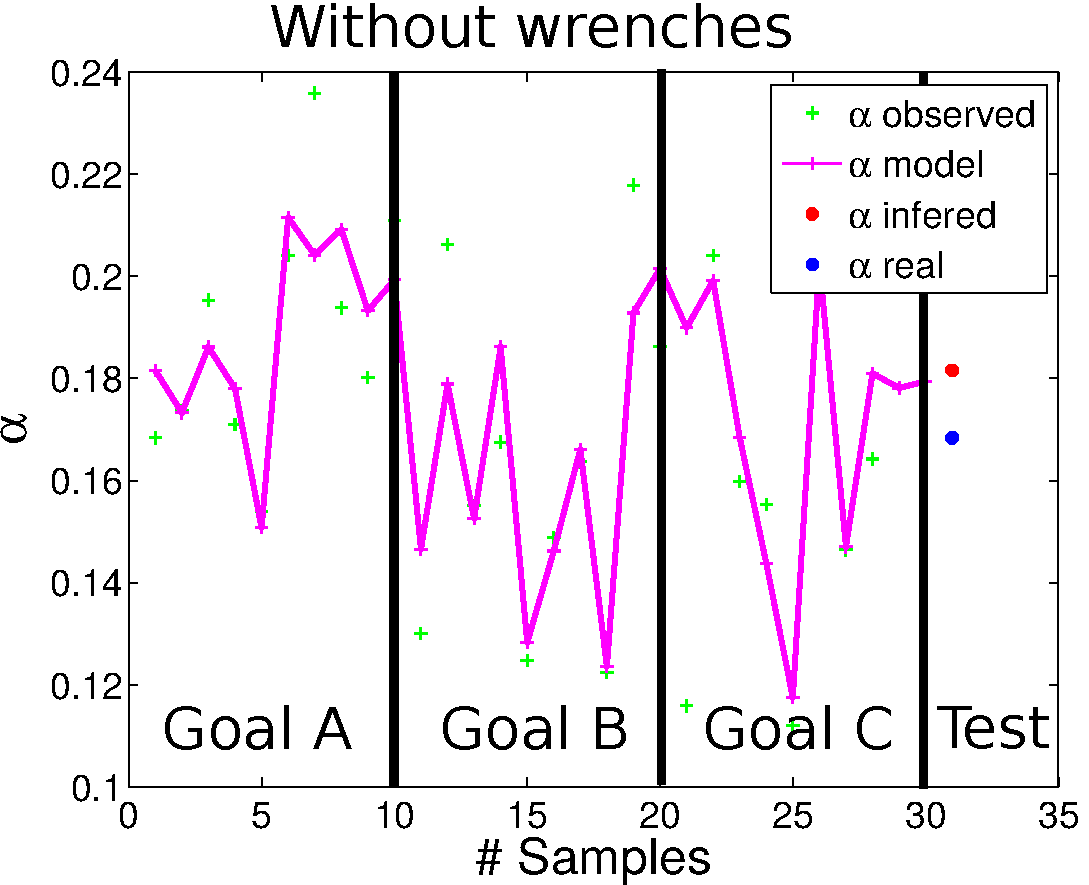
\includegraphics[width = 8cm]{img/realalphaModel.pdf} 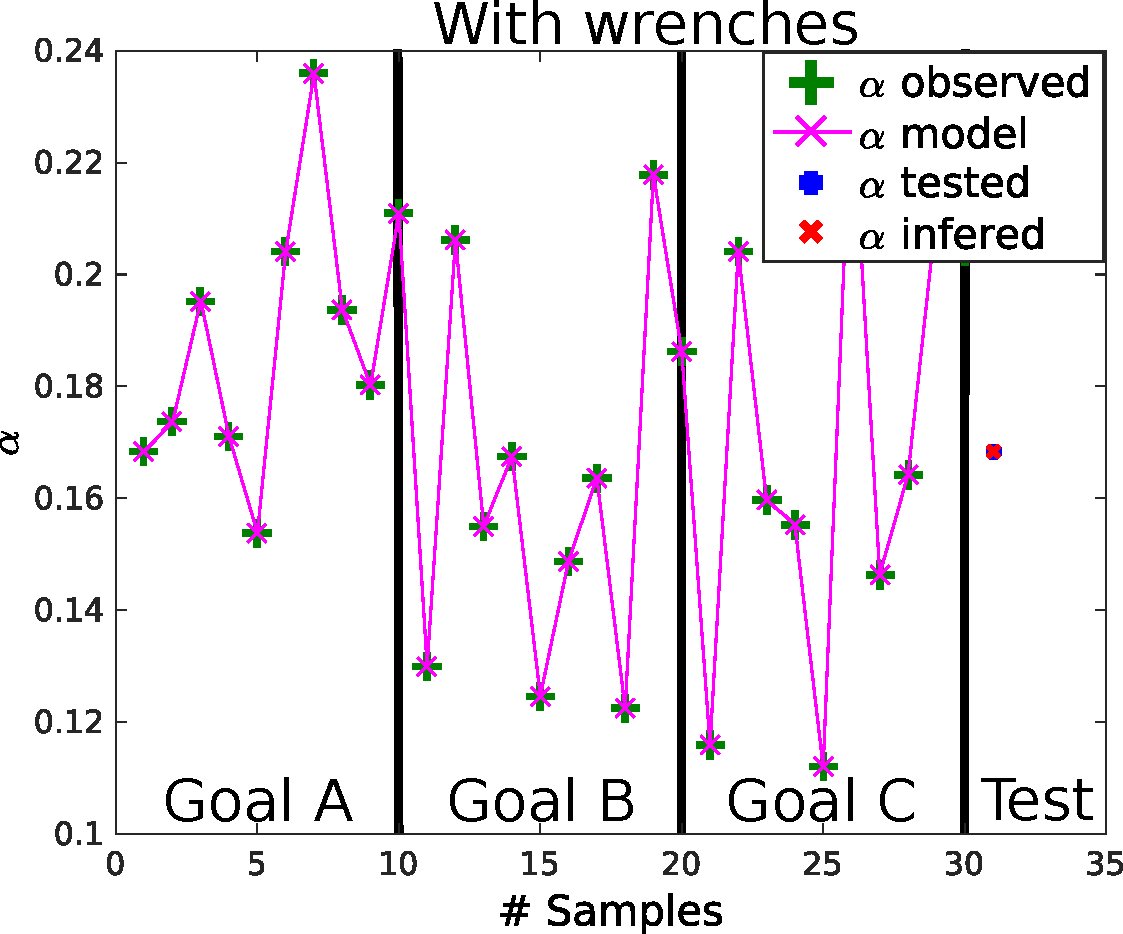
\includegraphics[width = 8cm]{img/alphaInfWithForces.pdf} 
%\caption{$\alpha$ model with (left) and without (right) wrenches. In pink, the $\alpha$ model based on the $\alpha$ set of the learning trajectories; in green, their real values; in red, the $\hat{\alpha}$ expectation of the test trajecory; and in blue its real value.
%}
%\label{fig:realalphaModel}
%\end{figure}

%Figure \ref{fig:realalphaModel} represents some $\alpha$ estimation using the learned model. On the left when the model doesn't contain wrench information, on the right with wrench information. The green crosses represent the $\alpha$ set of the learning trajectories, and the pink crosses the estimation done by the model based on this set. The $10$ first crosses are the $\alpha$ set of the first ProMP, the $10$ following the ones of the second ProMP and the last $10$ crosses the ones for the third ProMP. Finally, the red cross is the $\hat{\alpha}$ estimation of the test trajectory and the blue cross the real $\alpha$ of this test trajectory. We can see that with wrench information, the $\alpha$ estimation is really accurate.

\begin{figure}[!h]
\centering
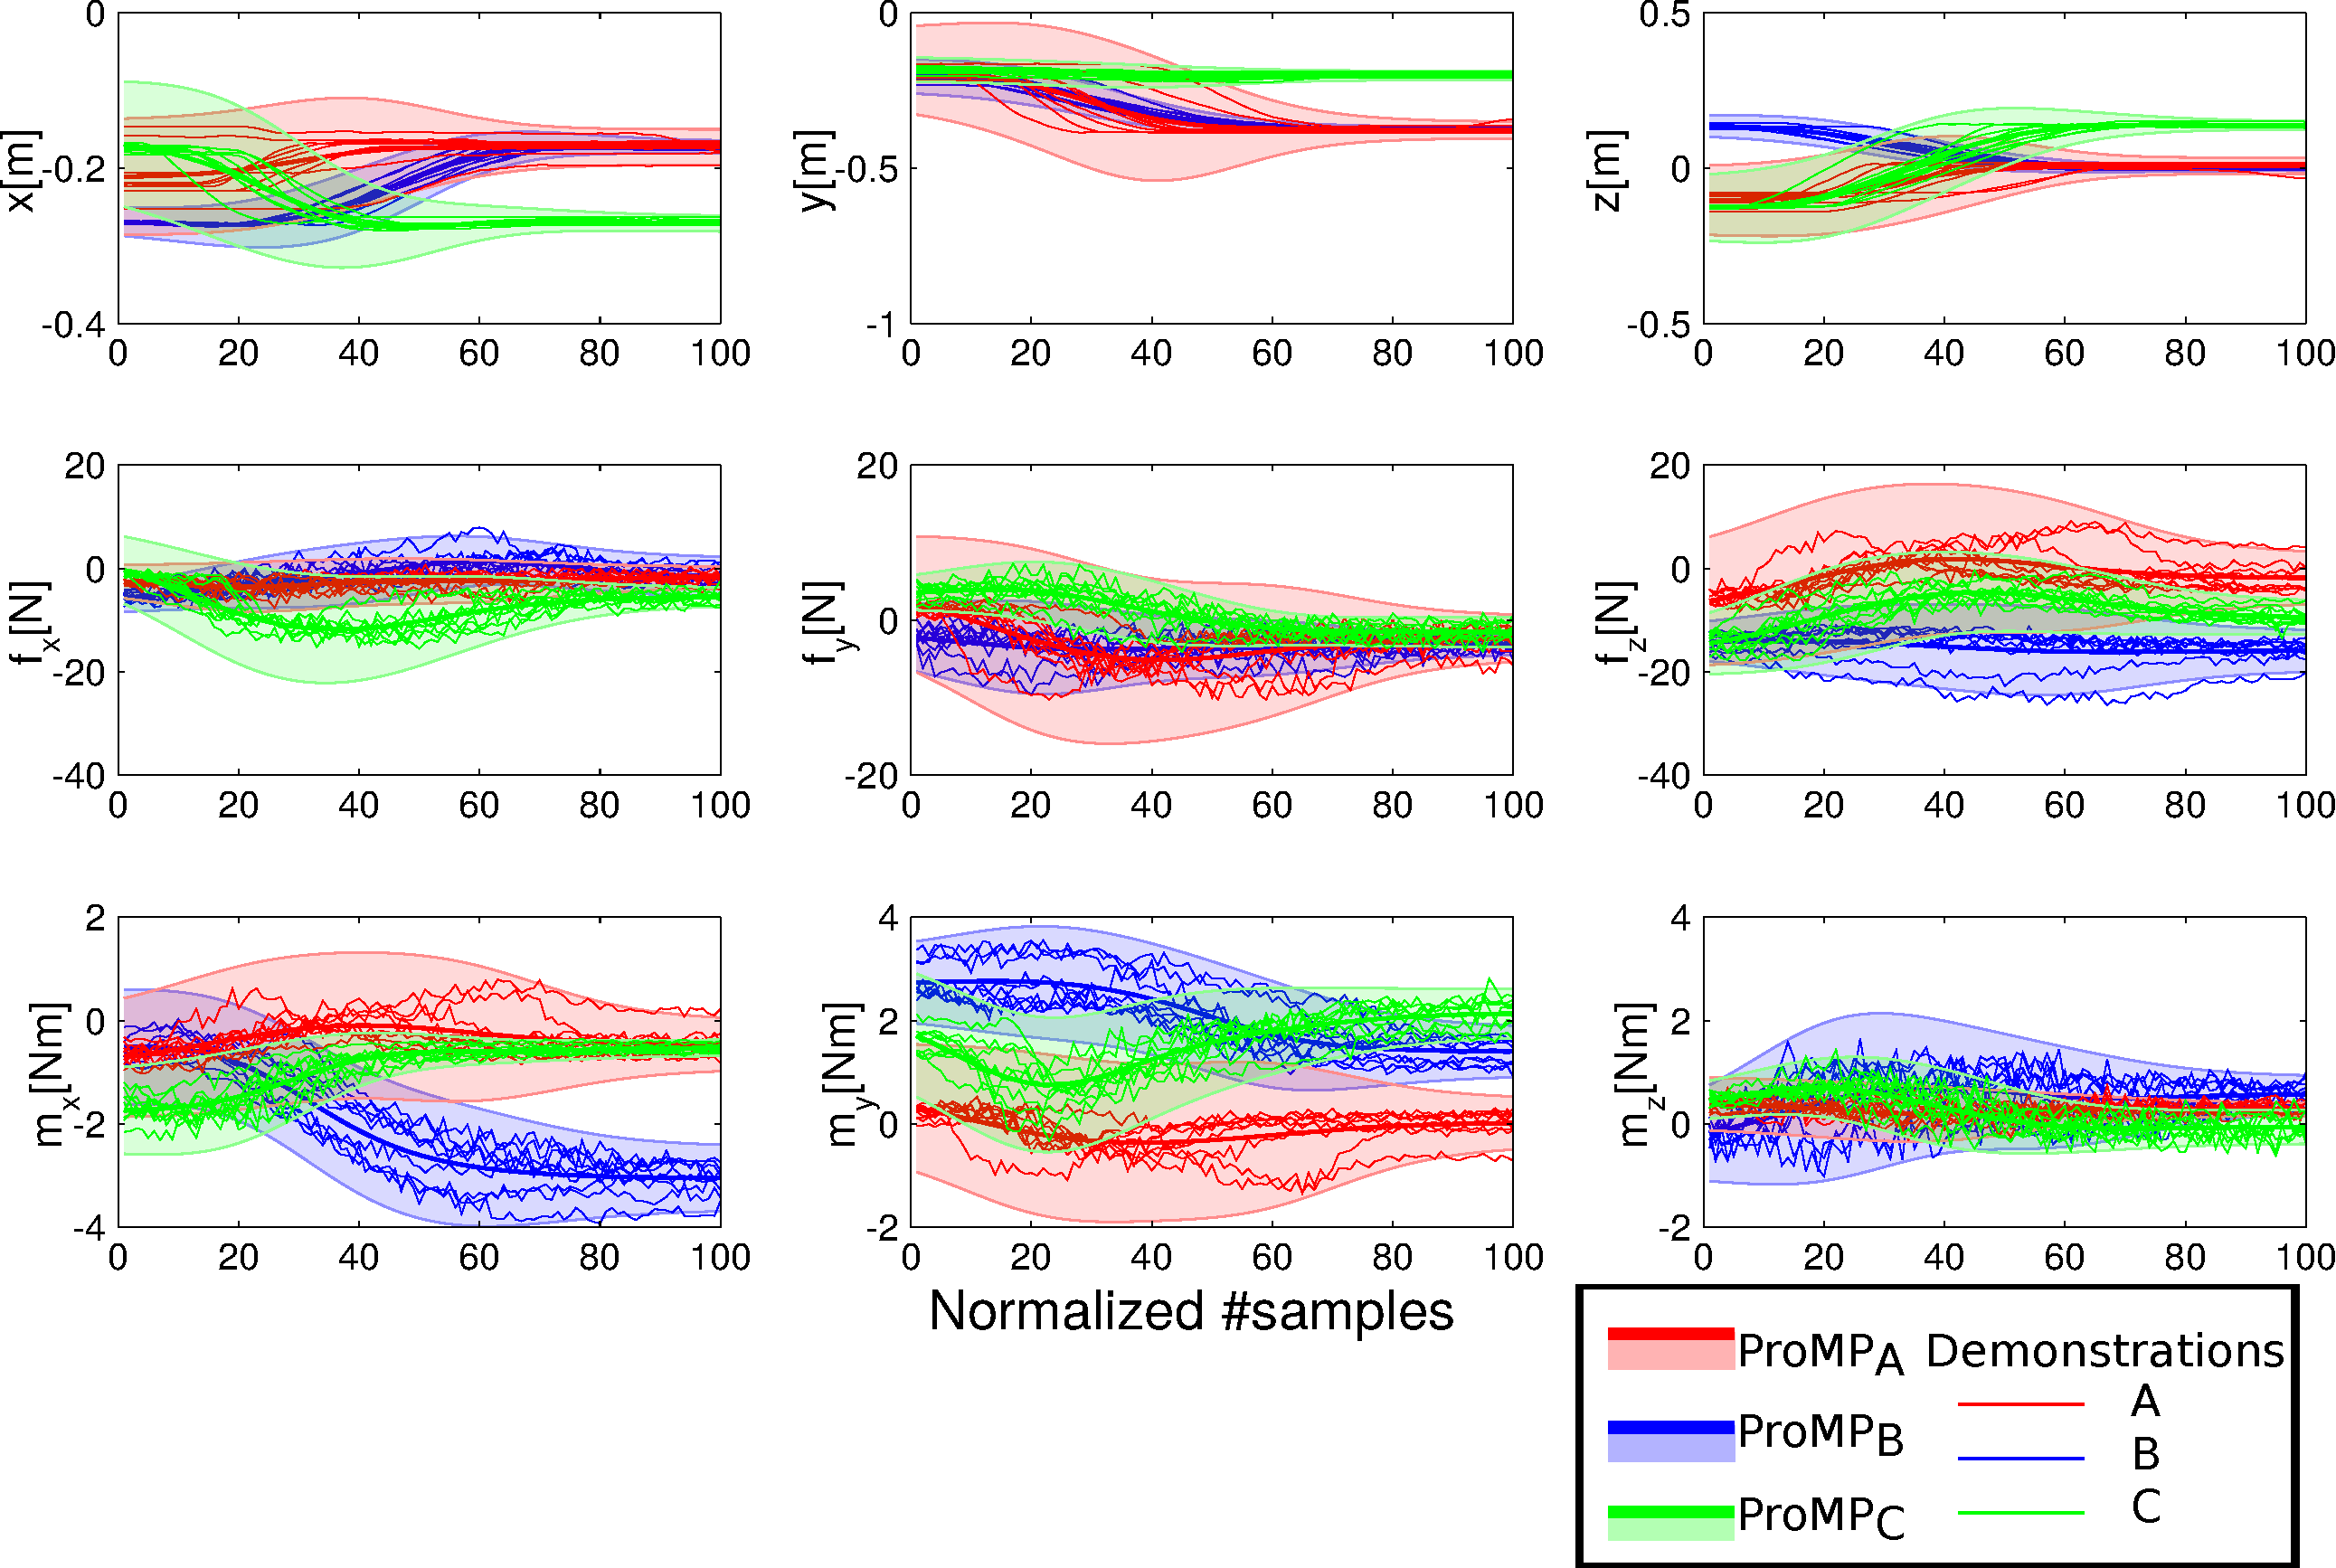
\includegraphics[height = 10cm]{img/realDistribution.pdf} 
\caption{The ProMPs learned by the robot from the demonstrations of Figure \ref{fig:realAppli}.}
\label{fig:realDistribution}
\end{figure}

\begin{figure}[!h]
\centering
{
\textcolor{red}{A}\\
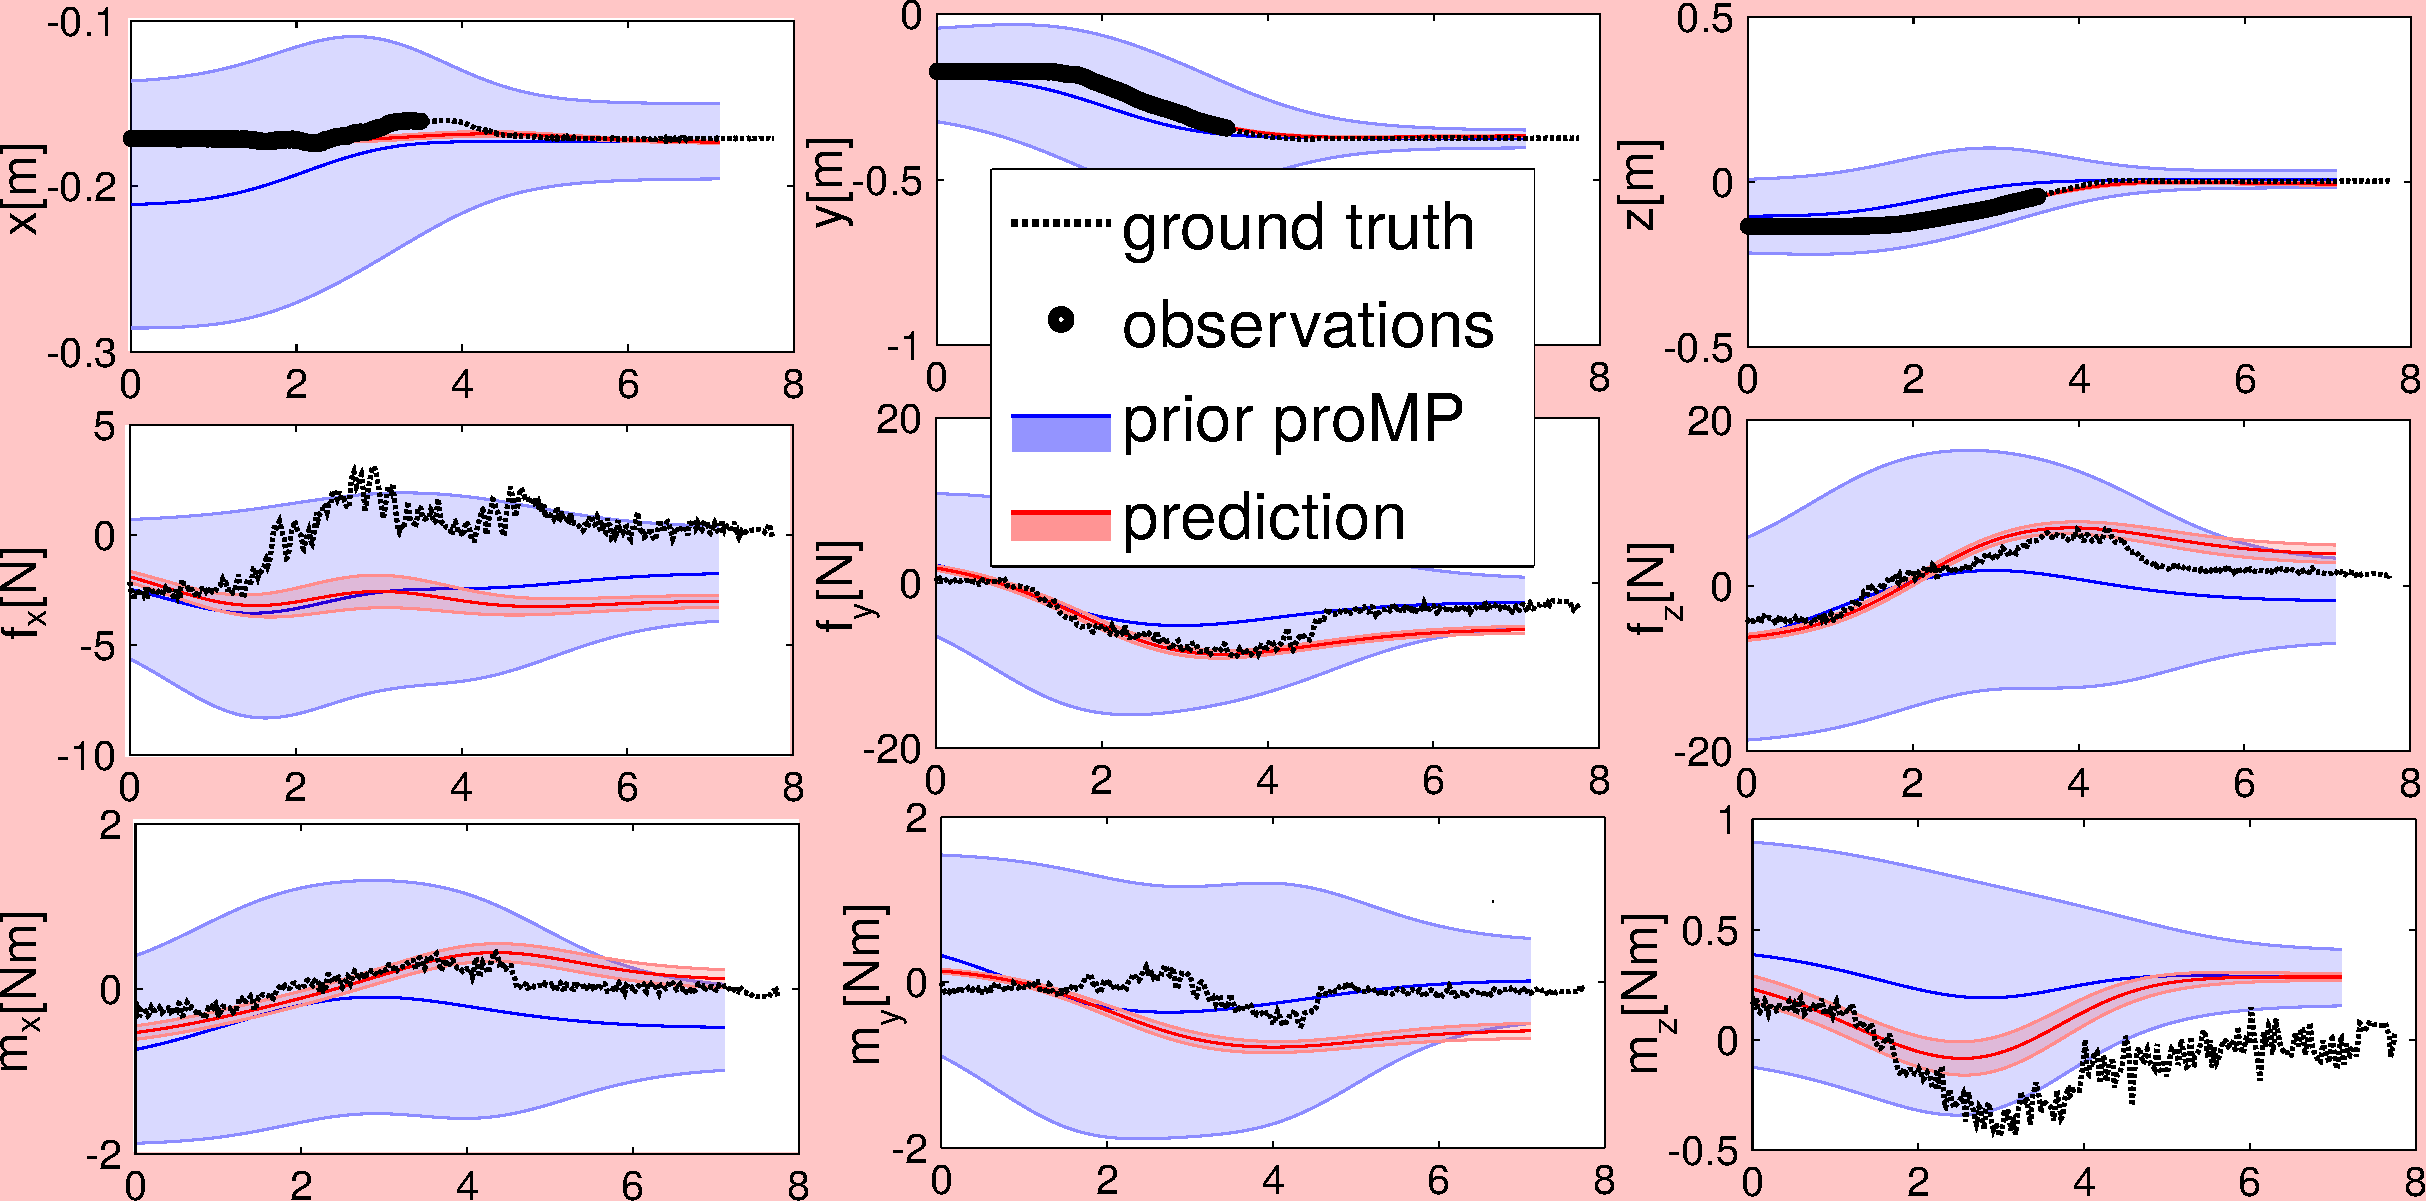
\includegraphics[width=15cm]{img/infA.pdf}\\
%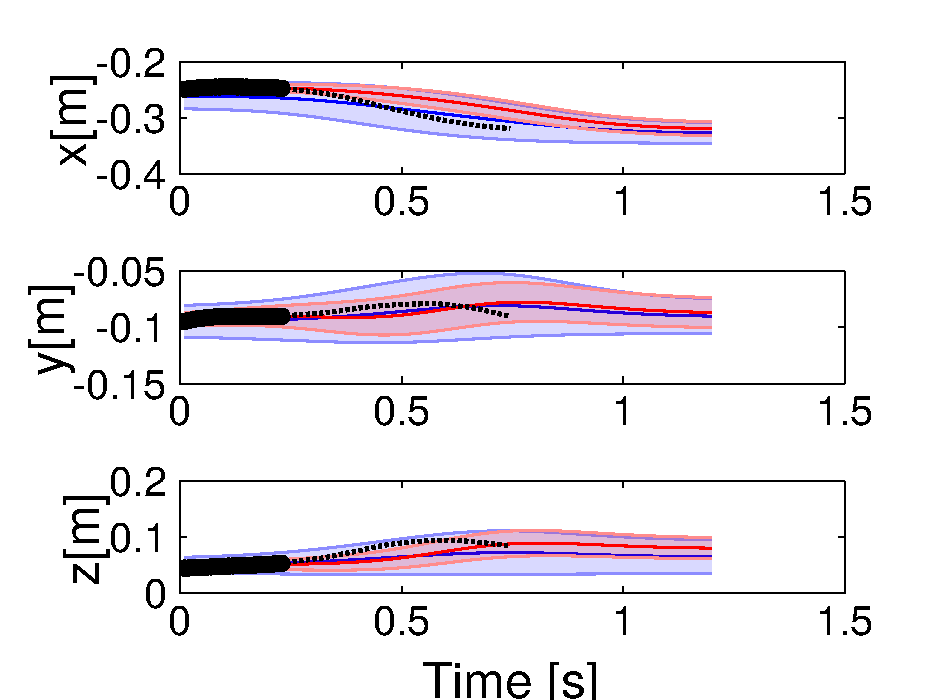
\includegraphics[width=\hsize /3]{img/infData3D/bottom30.pdf}
\textcolor{blue}{B}\\
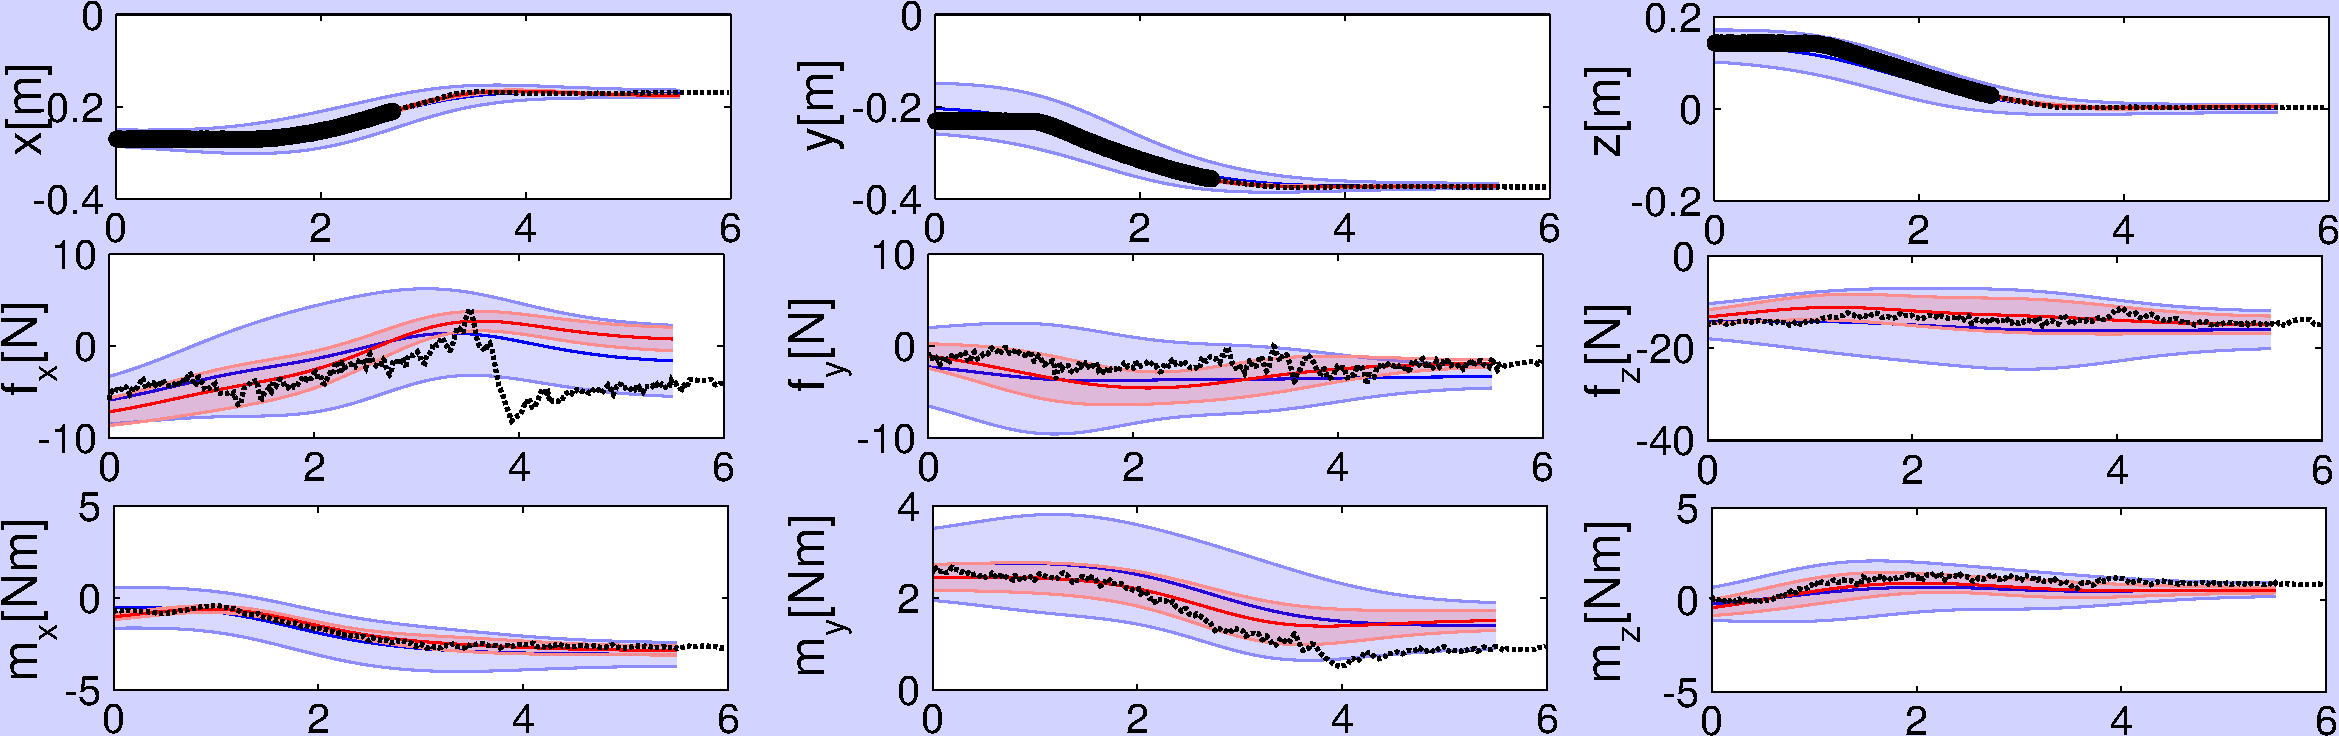
\includegraphics[width=15cm]{img/infb.pdf}\\
%%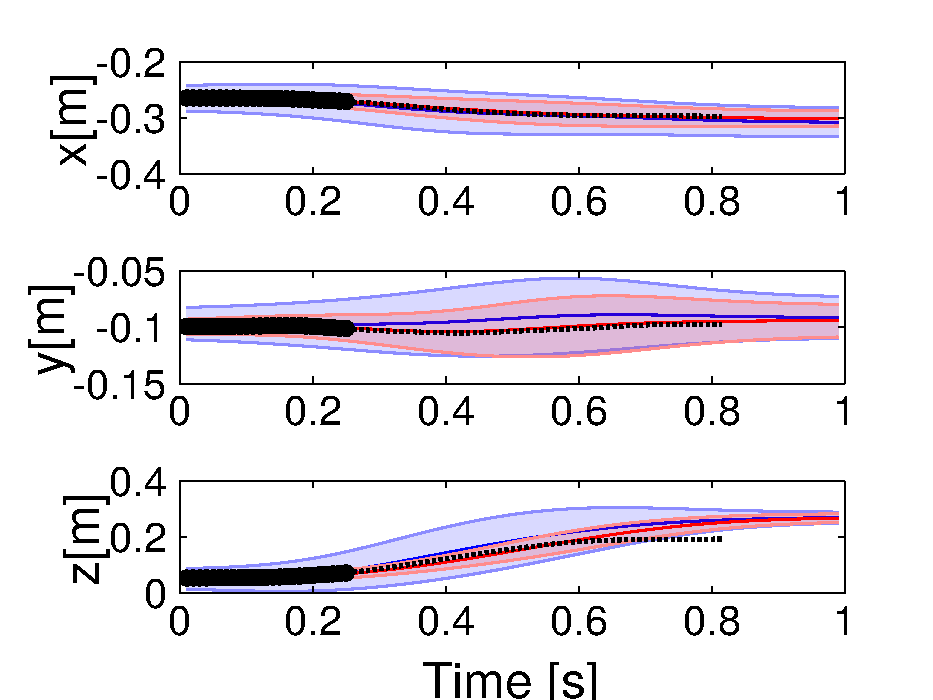
\includegraphics[width=\hsize /3]{img/infData3D/middle30Err.pdf}
\textcolor{green}{C}\\
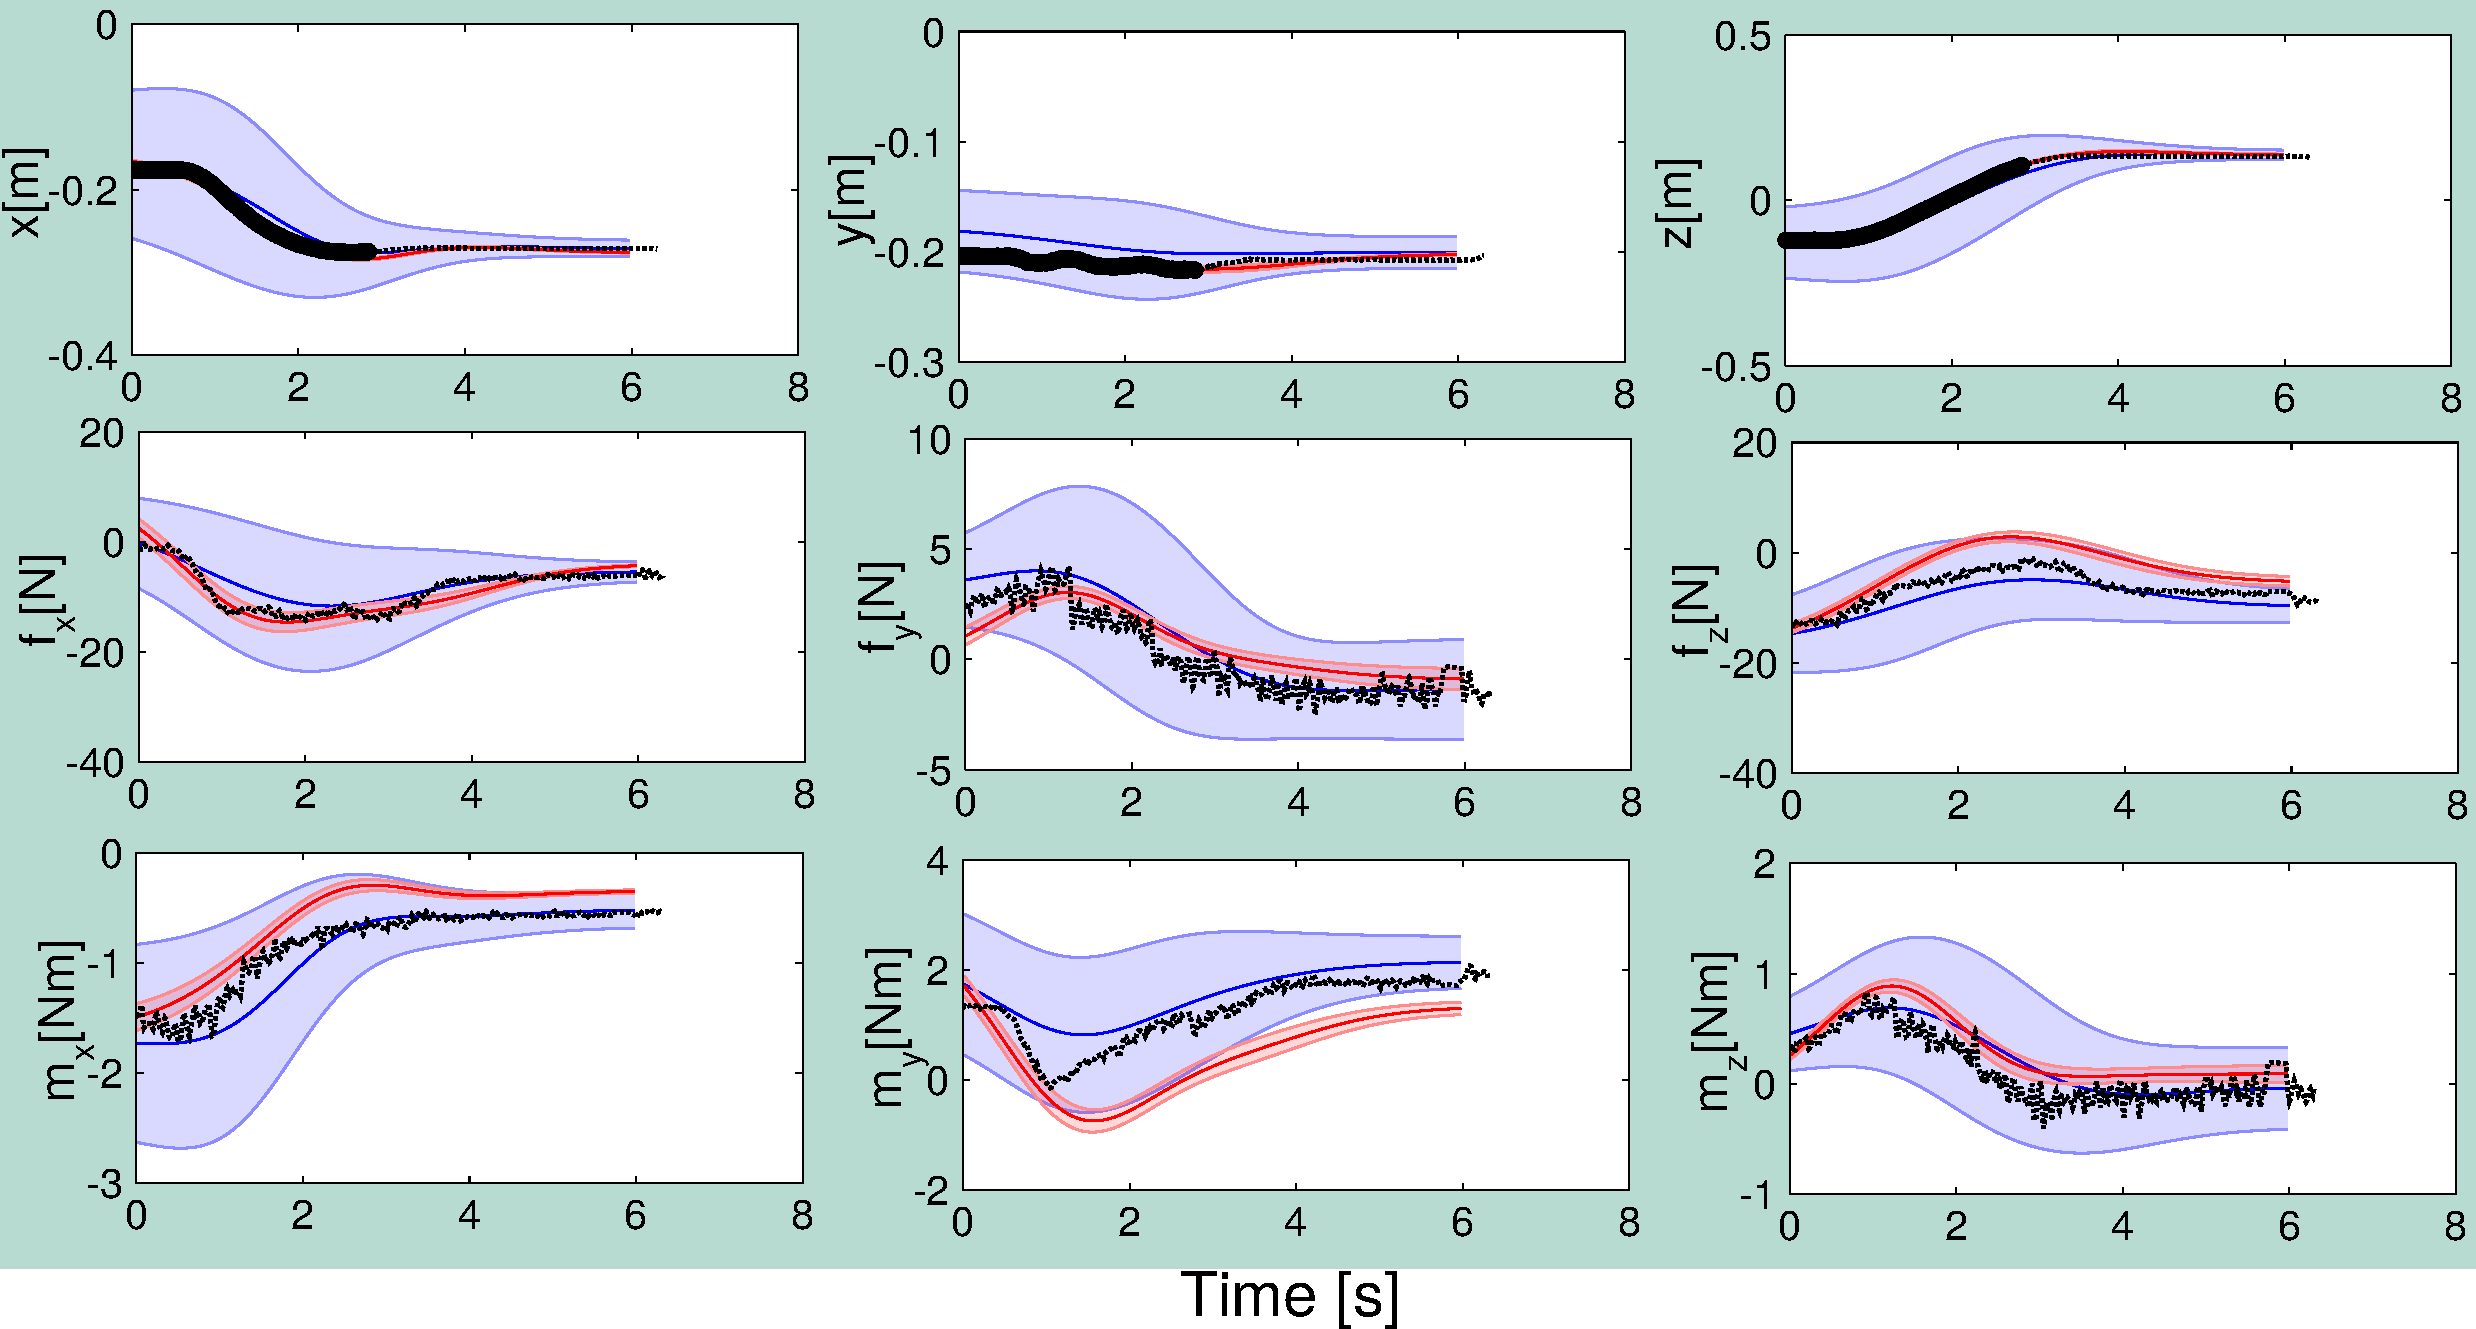
\includegraphics[width=15cm]{img/infc.pdf}\\
%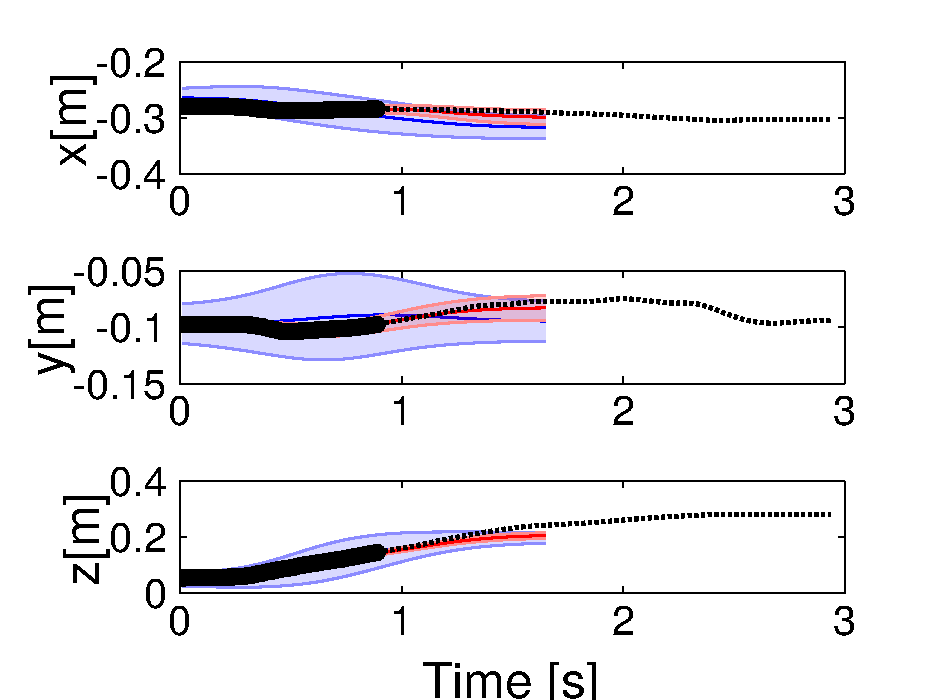
\includegraphics[width=\hsize /3]{img/infData3D/top30.pdf}
}
\caption{The prediction of the future trajectory from the learned ProMPs computed from the position information for the  3-targets dataset on the real iCub (Figure \ref{fig:realDistribution}) after 40\% of observations.}
\label{fig:realTrajectoriesPredictions}
\end{figure}

Then, the inference of the trajectory's target is performed. 
Figure~\ref{fig:realTrajectoriesPredictions} represents the inference of the three tested trajectories when wrench information is not used by the robot to infer the trajectory. 
\rev{To realize this figure, with the comparison between the predicted trajectory and the ground truth, we applied our algorithm offline. In fact, it is not possible at time $t$ to have the ground truth of the trajectory intended by the human from $t+1$ to $t_f$: even if we would tell to the human in advance the goal that he/she must reach for, the trajectory to reach that goal could vary. So, for the purpose of these figures and comparisons with the ground truth, we show here the offline evaluation: we select one demonstrated task trajectory from the test set (not the training set used to learn the ProMP) as ground truth, and imagine that this is the intended trajectory.
In Figure~\ref{fig:realTrajectoriesPredictions}, the ground truth is shown in black, whereas the portion of this trajectory that is fed to the inference, and that corresponds to the ``early observations'', is represented with bigger black circles.
}
%\rev{These tests have been done on a test base, that contains some whole-trajectories guided by the user. Then, we give to the program only a partial trajectory composed on 40\% of the recorded trajectory. The ground truth (\textit{e.g.} the total-trajectories of the test base) are represented in the figure in black. The partial-trajectories, that are known by the software are represented with the black circles.} 
We can see that the inference of the Cartesian position is correct, although we can see an error of about $1$ second of the estimated duration time for the last trial. Also, the wrench inference is not accurate. We can assume that it is: because the robot infers the trajectory using only position information without wrench information, or because the wrenches' variation is not correlated to the position variation.
To improve this result, we can make the inference using wrench in addition to Cartesian position information, as shown in Figure~\ref{fig:realTrajectoriesPredictionsWithForces}. We can see in this Figure that the estimation of the trajectory's duration is accurate. The disavantage is that the inference of the Cartesian position is less accurate because the posterior distribution computation makes a trade-off between fitting Cartesian position and wrench early observations. Moreover, to allow a correct inference using wrench information, the noise expectation must be increased to consider forces. \footnote{In future versions, we will include the possibility to have different noise models for the observations, \textit{e.g.} we will have $\Sigma_\Xi^o = \left[
\begin{array}{c c}
\Sigma_X  & 0\\  
0 &\Sigma_F \\
\end{array}\right]$. We will therefore set a bigger covariance for the wrench information than for the position information.}


%allow to have different expectation noises according to the data type
%\textcolor{blue}{expectation noises [Obs.: Is “noise
%expectation” or “expectation noise” the same as “observation noise”?]}
%\textcolor{purple}{@marco: i didn't understand your question but tell me if it is more clear now with the following parenthesis} 


To confirm these results, we analyzed the trajectory inference and $\alpha$ estimation considering different percentages of each trajectory as observed data ($30$ to $90\%$). For each percentage, we performed $20$ tests, with and without force information.


In Figure~\ref{fig:errBoxWithWithoutForces}, each box-plot represents errors for $20$ tests.
On the top, the error criterion is the average distance between the inferred trajectory and the real one. We can see that the inference of Cartesian end-effector trajectory is more accurate without wrench information.
On the bottom, the error criterion is the distance between the estimated $\alpha$ and the real one. We can see that using wrench information, the estimation of the $\alpha$ is more accurate.
Thus, these two graphs confirm what we assumed from Figures~\ref{fig:realTrajectoriesPredictions} and ~\ref{fig:realTrajectoriesPredictionsWithForces}. 

\rev{Median, mean and variance of the prediction errors, computed with the normalized root-mean-square error (NRMSE) are reported in Table~\ref{table:statsError}. 
The prediction error for the time modulation is a scalar: $|\alpha_{\textrm{prediction}} - \alpha_{\textrm{real}} |$.   
The prediction error for the trajectory is computed by the NRMSE of $| \Xi_{\textrm{prediction}} - \Xi_{\textrm{real}}  |$.}

In future upgrades for this application, we will probably use the wrench information only to estimate the time modulation parameter $\alpha$, to have both the best inference of the intended trajectory and the best estimation of the time modulation parameter to combine the benefits of inference with and without wrench information.


\rev{
Table~\ref{table:statsError} also reports the average time for computing the prediction of both time modulation and posterior distribution.  The computation were performed in Matlab, on a single core laptop (no parallelization). While the computation time for the case ``without wrenches'' is fine for real-time application, using the wrench information delays the prediction and represents a limit for real-time applications if fast decisions have to taken by the robot. Computation time will be improved in the future works, with the implementation of the prediction in an iterative way.
}

%or change the tolerance interval of accepted wrenches \todo{as represented in figure\ref{}}.

\begin{figure}[!h]
\centering
{
\textcolor{red}{A}\\
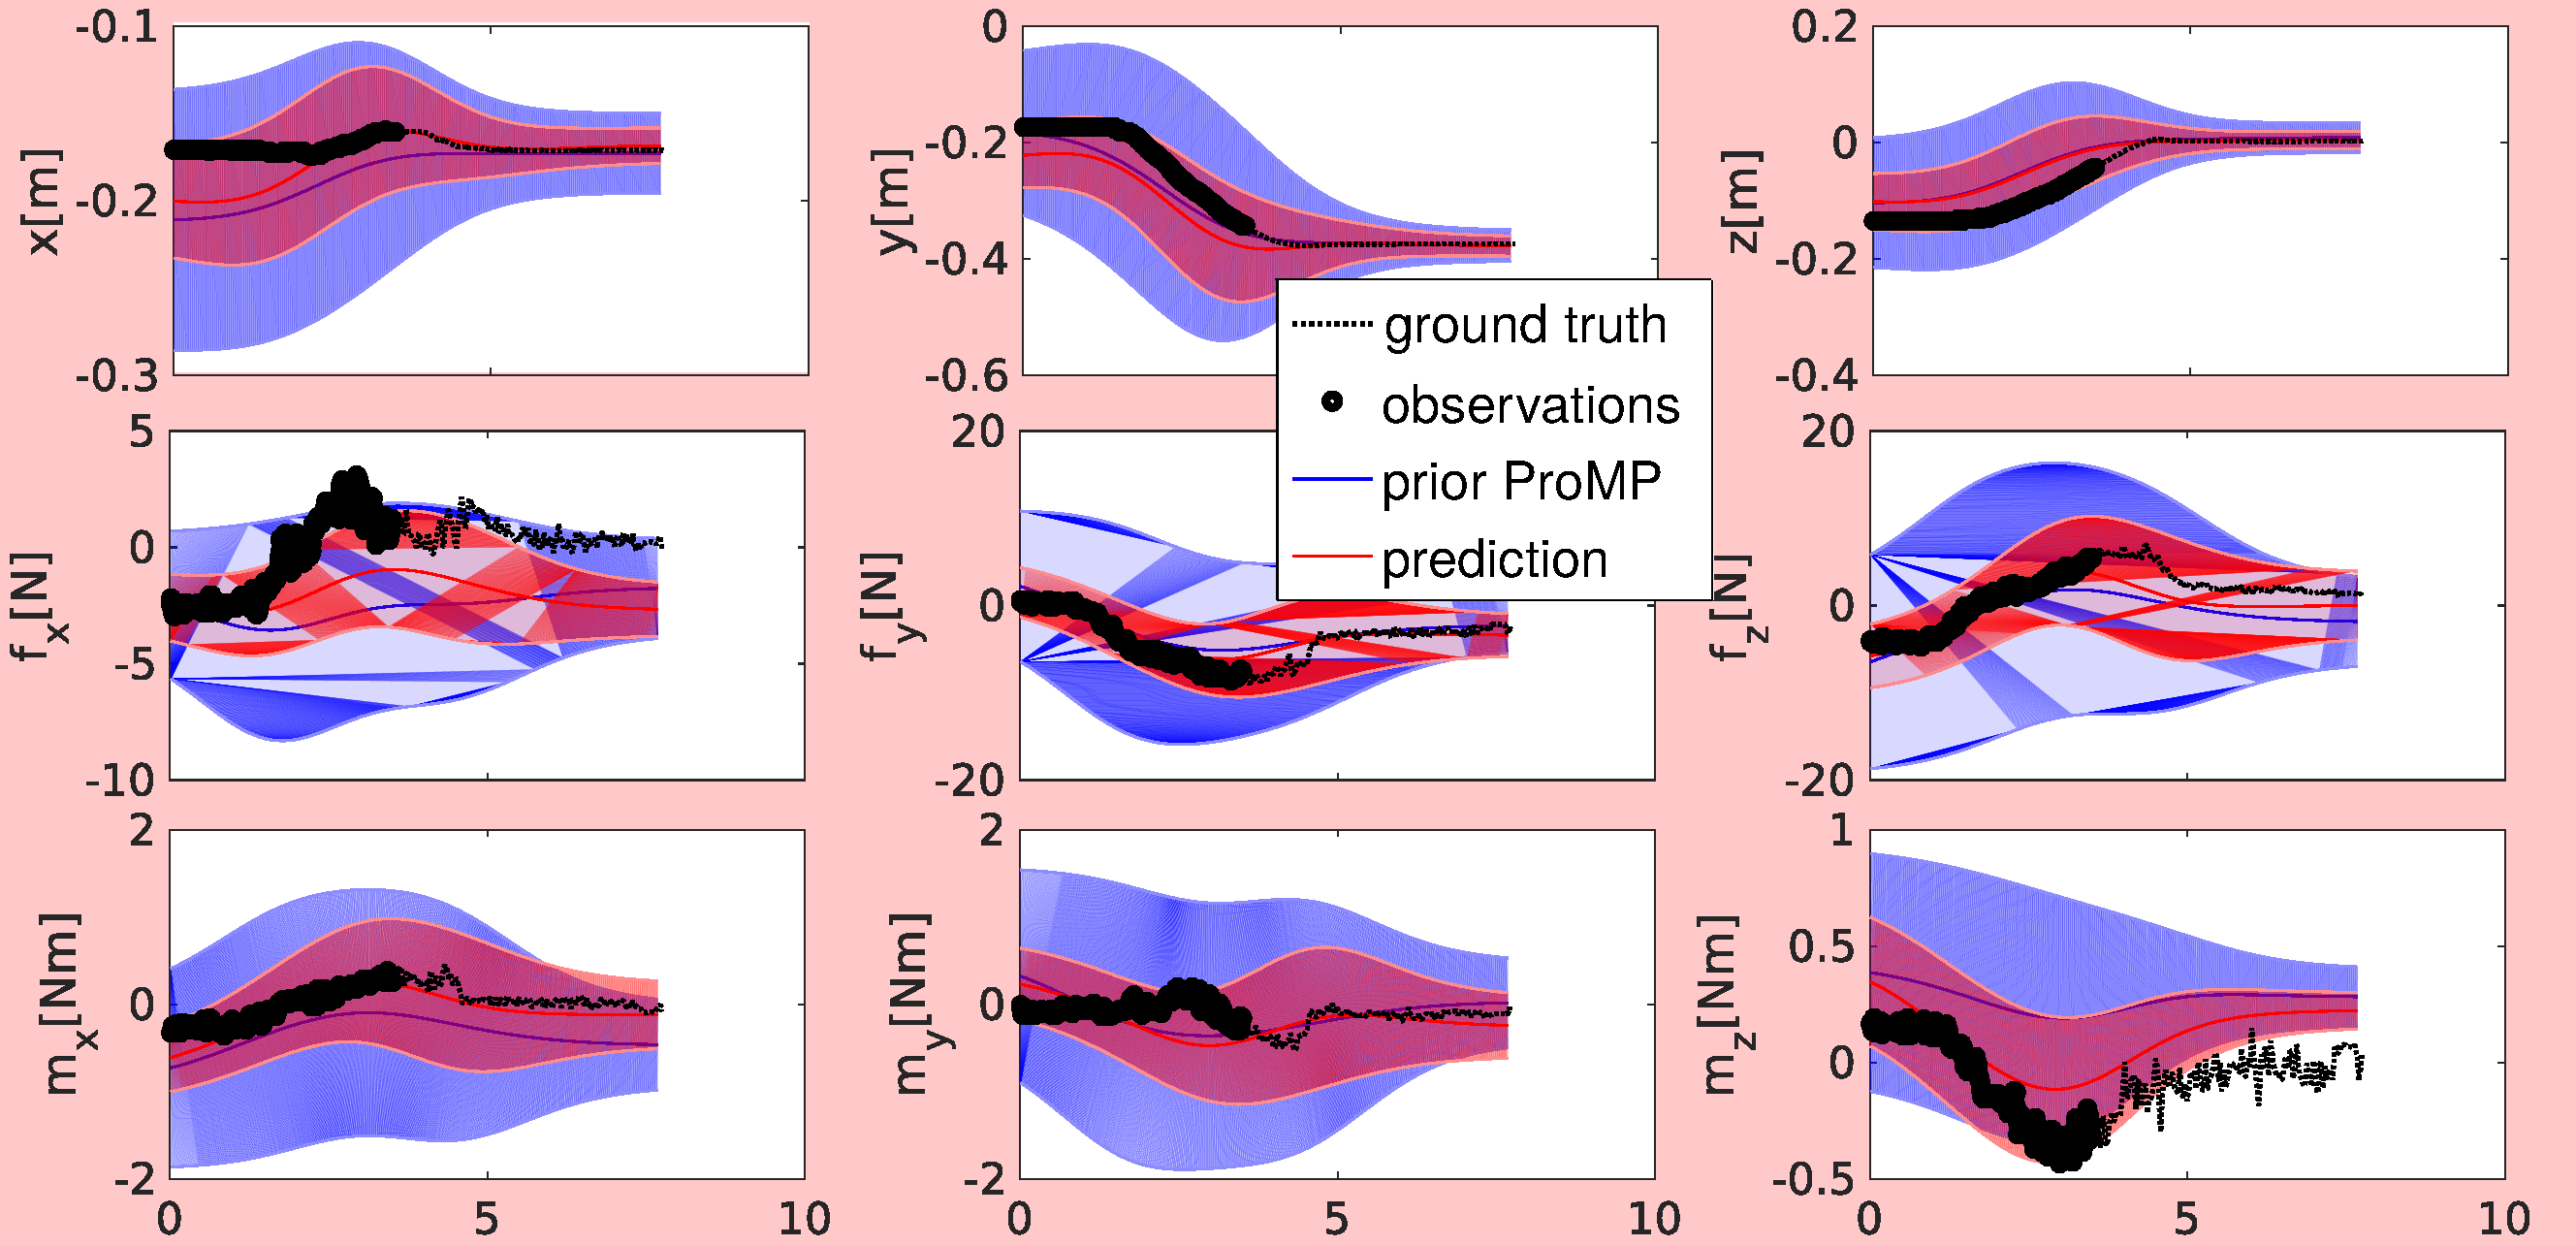
\includegraphics[width=14cm]{img/withWrenchInfA.pdf}\\
\textcolor{blue}{B}\\
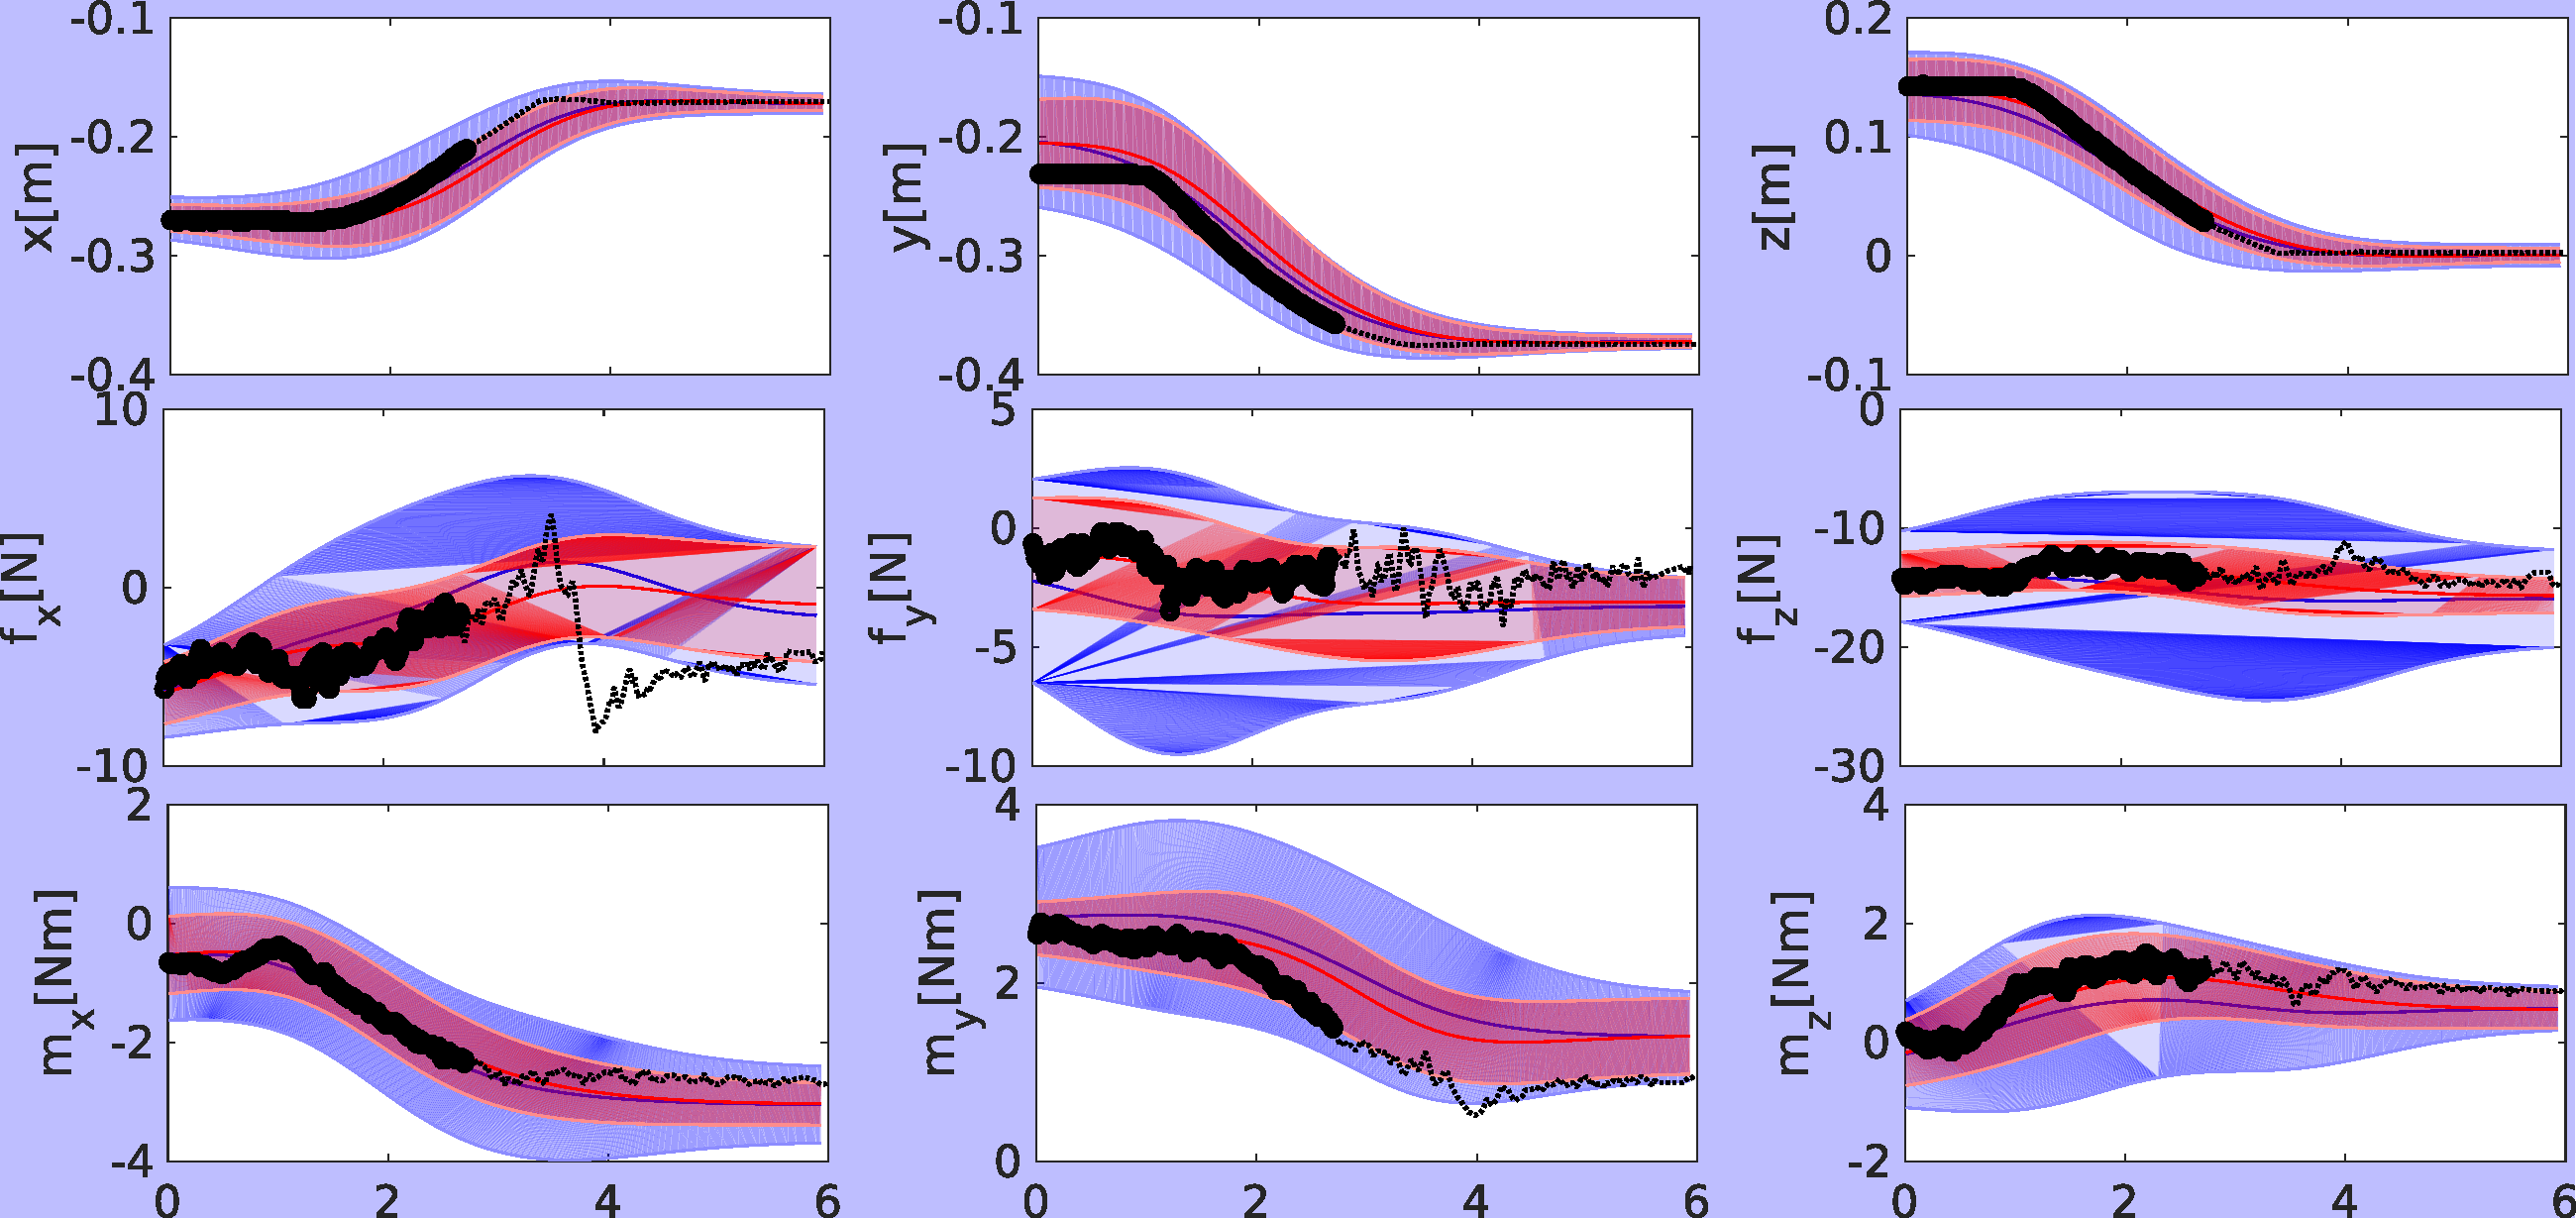
\includegraphics[width=14cm]{img/withWrenchInfB.pdf}\\
\textcolor{green}{C}\\
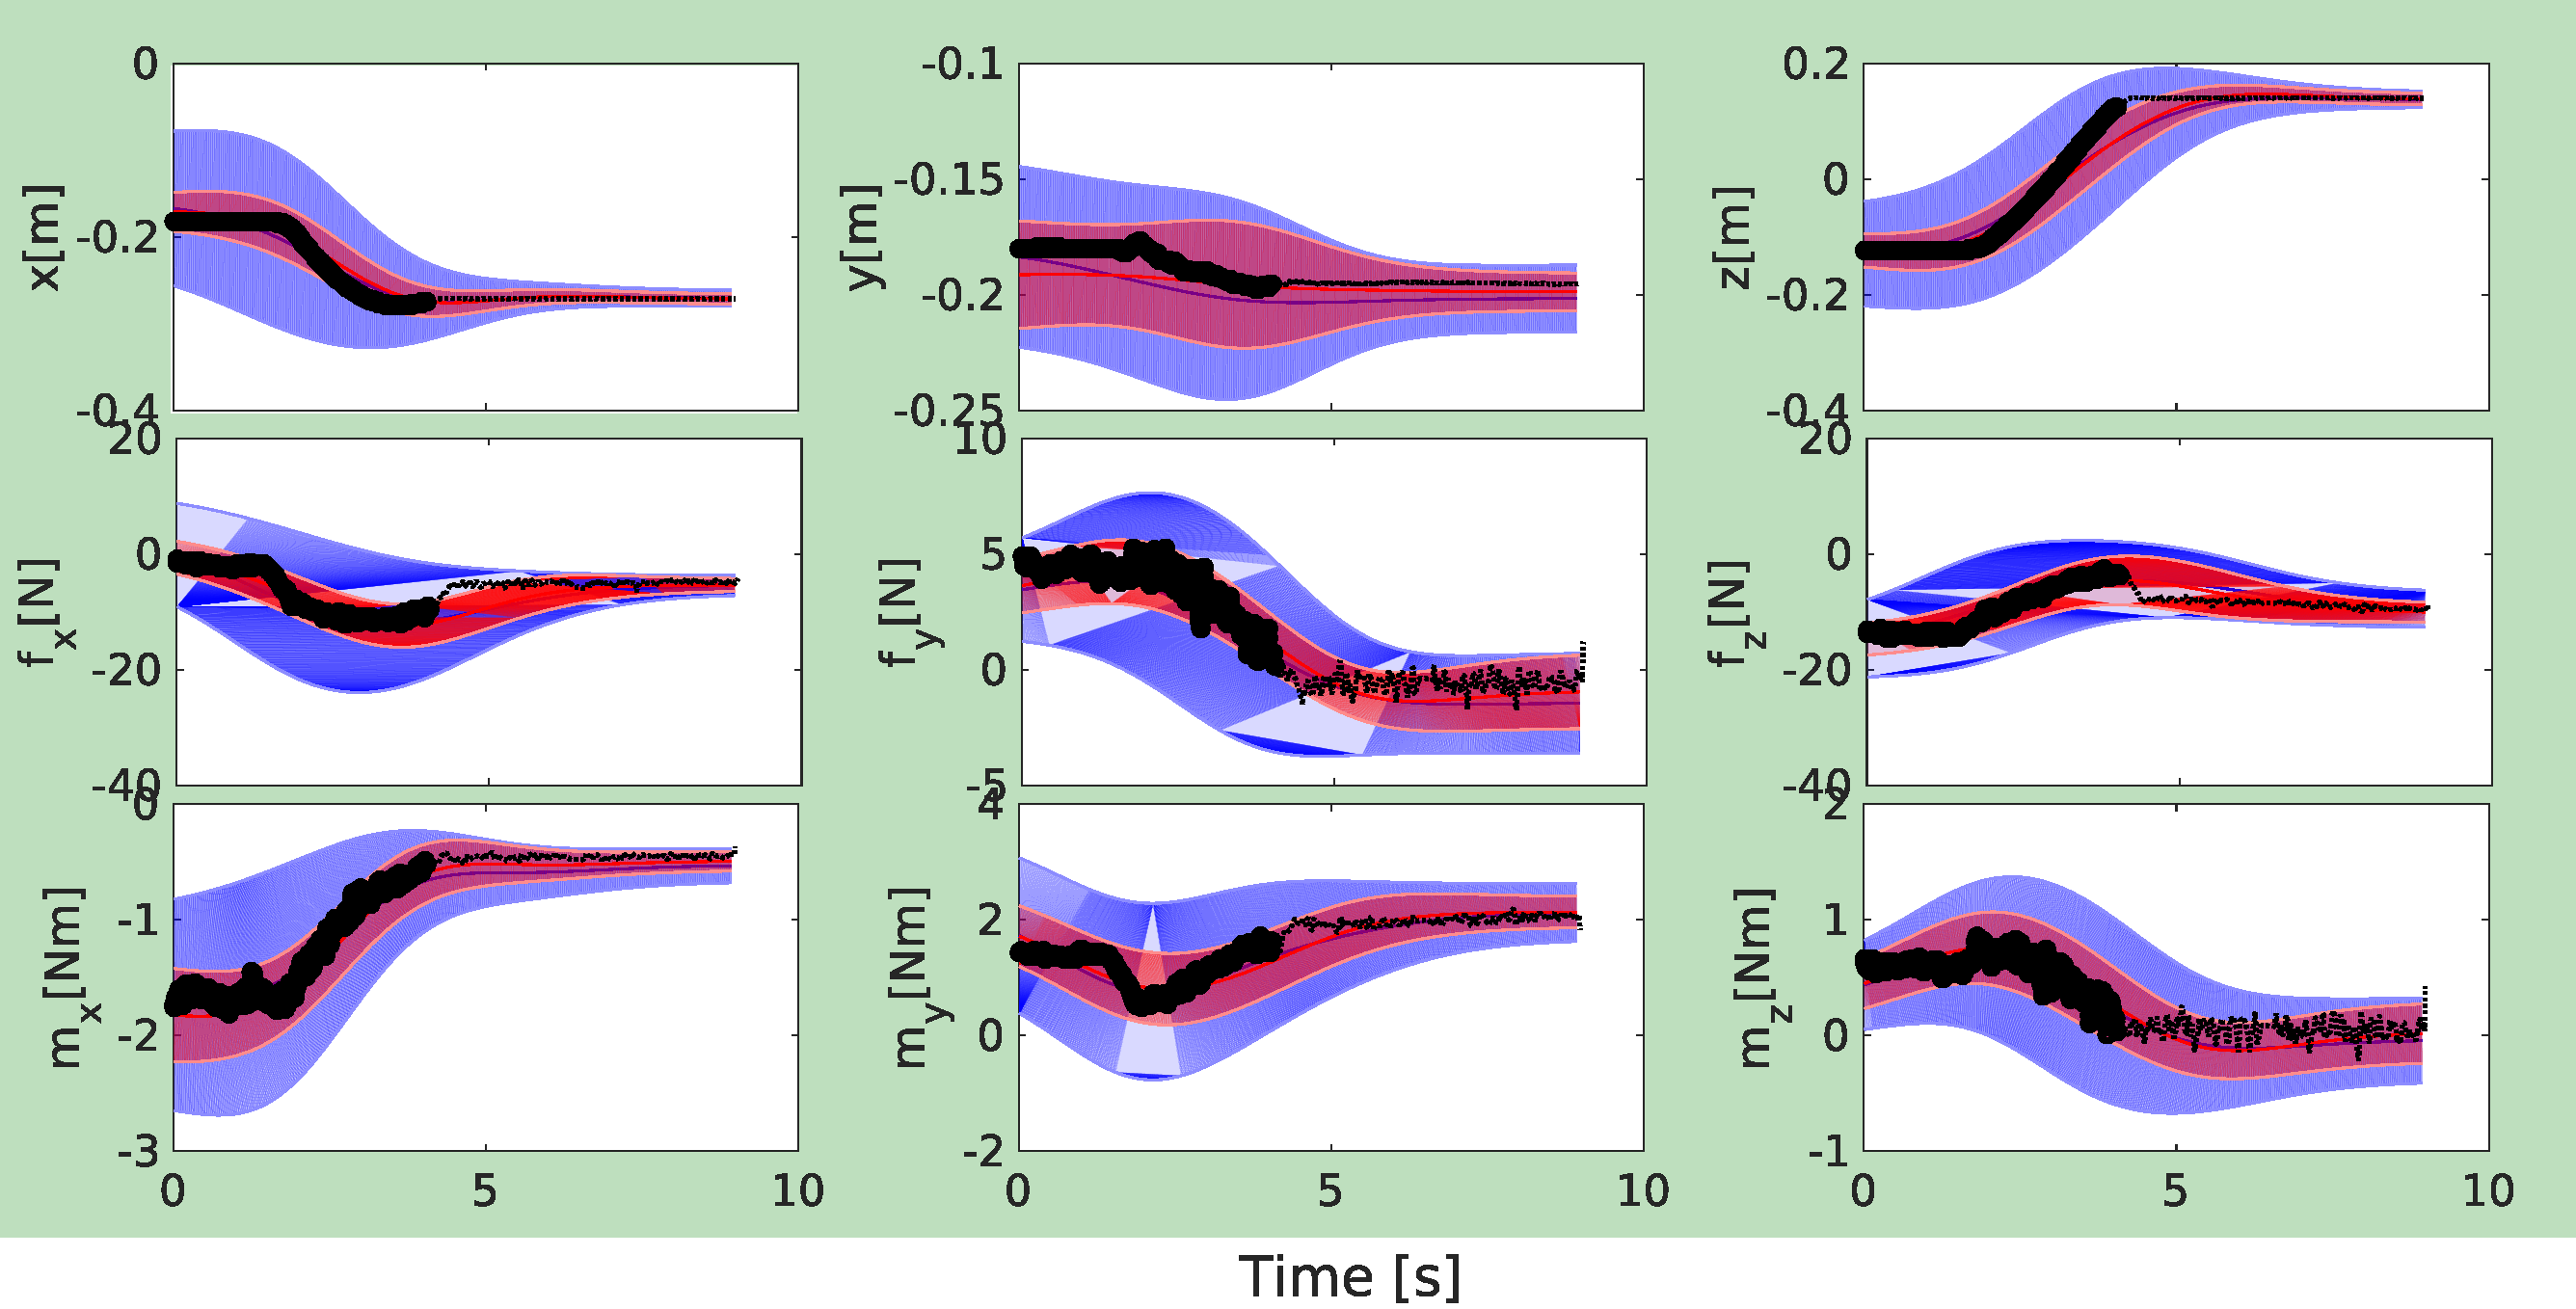
\includegraphics[width=14cm]{img/withWrenchInfC.pdf}\\
%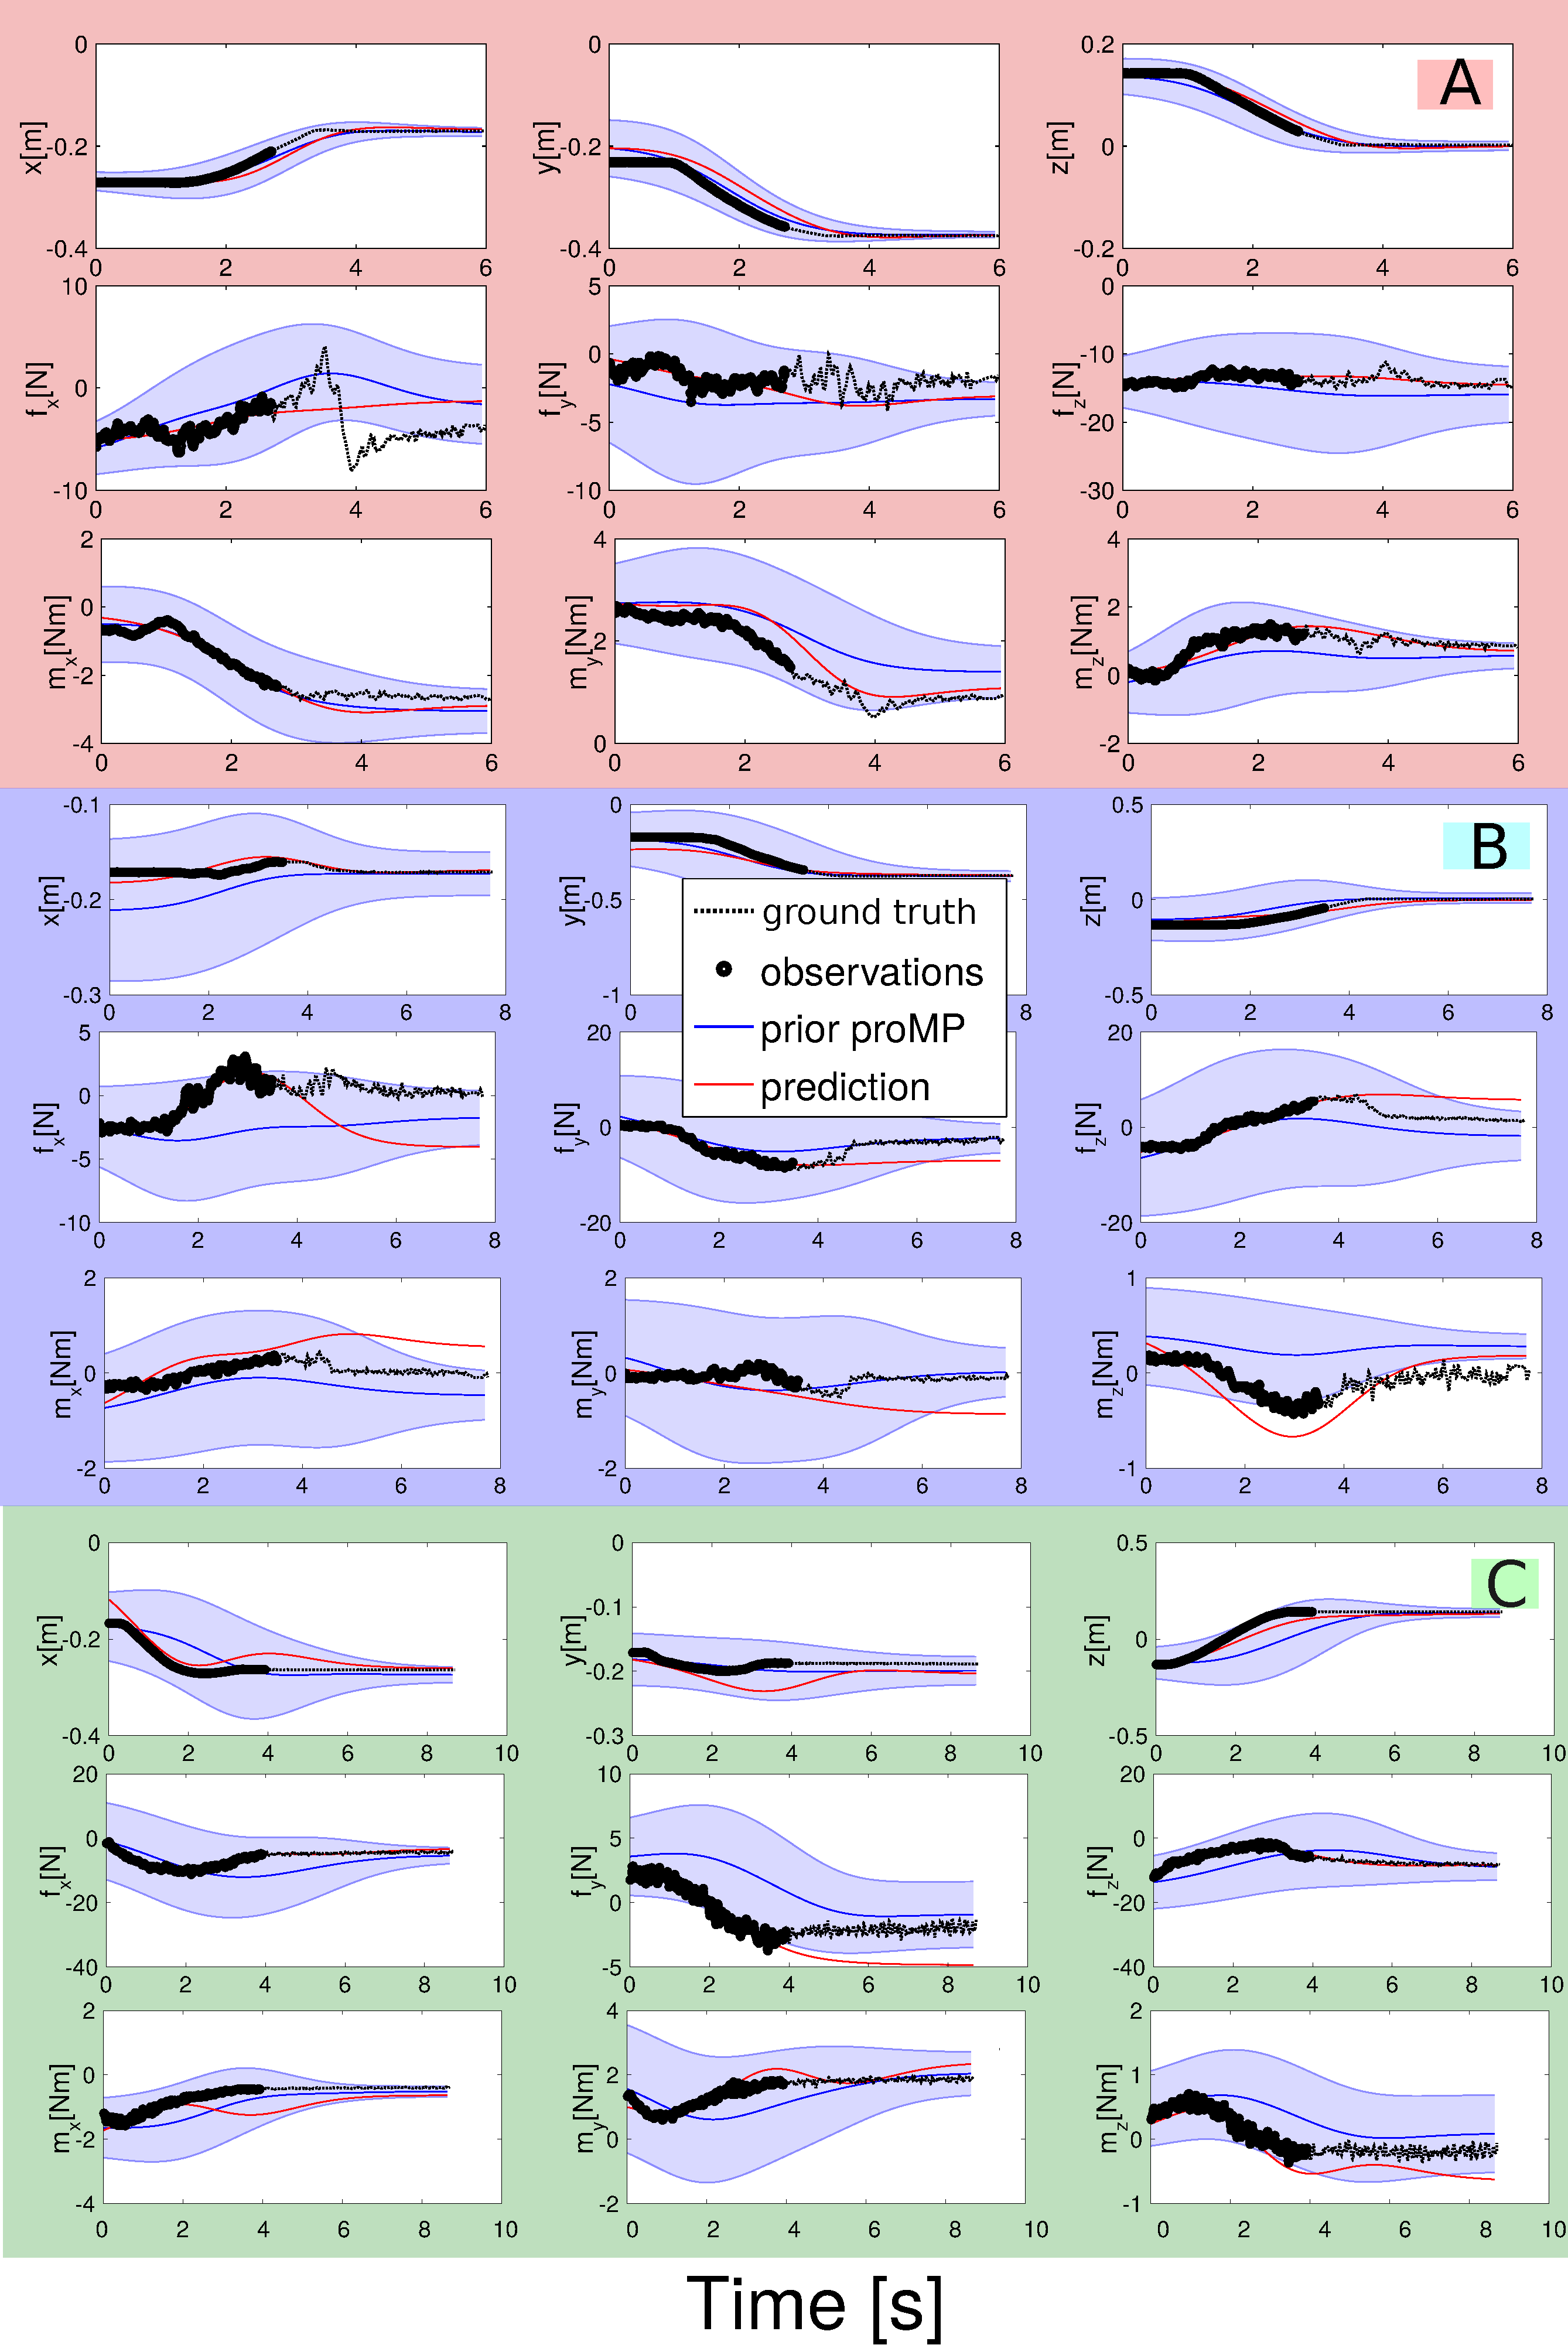
\includegraphics[height=20cm]{img/infUseForces.pdf}
}
\caption{The prediction of the future trajectory from the learned ProMPs computed from the position and wrench information for the 3-targets dataset on the real iCub (Figure \ref{fig:realDistribution}) after 40\% of observations.}
\label{fig:realTrajectoriesPredictionsWithForces}
\end{figure}


\begin{figure}[!h]
\centering
{
\includegraphics[width=12cm]{img/errBoxWithWithoutForces.pdf}\\
\includegraphics[width=12cm]{img/boxAlphaErrorWithForces.pdf}
}
\caption{Trajectory prediction error (top) and time modulation estimation error (bottom) of the future trajectory with and without wrench information, for the 3-targets dataset on the real iCub (Figure \ref{fig:realDistribution}) with respect to the number of observed data points.}
\label{fig:errBoxWithWithoutForces}
\end{figure}

%\begin{table}
%\centering
%\begin{tabular}{|c|c|c|c|c|c|c|c|}
% \hline
% Percentage of observations & 30 & 40 & 50 & 60 & 70 & 80 & 90 \\
% \hline
% Trajectory prediction error &   &    &    &    &    &    &    \\
% \hline
% Time modulation prediction error & & & & & & & \\
% \hline
% Computation time for prediction & & & & & & & \\
% \hline
%\end{tabular}
%\caption{ \todo{ORIANE FILL IT}}
%\label{table:statsError}
%\end{table}

\begin{table}
\begin{center}
\color{blue}
\textbf{With wrenches}
\begin{tabular}{|p{3.6cm}|p{2cm}|c|c|c|c|}
  \hline 
   \% of observed data ($\simeq$ n. of samples) &  & \textbf{$30 (\simeq 180$)} & \textbf{$50 (\simeq 300$)} & \textbf{$70 (\simeq 419$)} & \textbf{$90 (\simeq 539$)}  \tabularnewline
  \hline
\multirow{3}{3cm}{Prediction error of time modulation} &  median& 2.26e-08 & 1.35e-08 & 3.61e-09 & 8.95e-09 \tabularnewline
 % \hline
  \cline{2-6} & mean & 4.26e-02 & 7.81e-09 & 2.19e-08 & 2.09e-08 \tabularnewline
 \cline{2-6} & variance & 1.08e-02 & 1.09e-16 & 5.44e-16 & 2.24e-16 \tabularnewline
  \hline
\multirow{3}{3cm}{Prediction error for the trajectory (NRMSE) [m]} &  median& 2.73e-01 & 5.51e-01 & 4.52e-01 & 5.38e-01 \tabularnewline
 % \hline
  \cline{2-6} & mean & 8.11e-01 & 5.86e-01 & 5.29e-01 & 3.42e-01 \tabularnewline
 \cline{2-6} & variance & 7.45e-01 & 1.36e-01 & 7.74e-02 & 2.93e-02 \tabularnewline
  \hline  
\multirow{2}{3cm}{Computation time [s]} &  mean & 0.25 & 0.74 & 1.92 & 3.59 \tabularnewline
 \cline{2-6} & variance & 0.01 & 0.27 & 2.77 & 4.81 \tabularnewline
 \hline
\end{tabular}

\vspace{0.4cm}
\textbf{Without wrenches}
\begin{tabular}{|p{3.6cm}|p{2cm}|c|c|c|c|}
  \hline 
   \% of observed data ($\simeq$ n. of samples) &  & \textbf{$30 (\simeq 180$)} & \textbf{$50 (\simeq 300$)} & \textbf{$70 (\simeq 419$)} & \textbf{$90 (\simeq 539$)}  \tabularnewline
  \hline
\multirow{3}{3cm}{Prediction error of time modulation} &  median& 1.19e-02 & 1.76e-02 & 1.74e-02 & 1.62e-02 \tabularnewline
  \cline{2-6} & mean & 2.81e-02 & 1.92e-02 & 2.45e-02 & 1.43e-02 \tabularnewline
 \cline{2-6} & variance & 9.51e-04 & 1.00e-04 & 3.37e-04 & 1.82e-04 \tabularnewline
  \hline
\multirow{3}{3cm}{Prediction error for the trajectory (NRMSE) [m]} &  median& 4.53e-02 & 4.73e-02 & 7.20e-02 & 6.20e-02 \tabularnewline
 % \hline
  \cline{2-6} & mean & 1.56e-01 & 7.36e-02 & 5.75e-02 & 4.29e-02 \tabularnewline
 \cline{2-6} & variance & 5.04e-02 & 1.80e-03 & 1.80e-03 & 6.0e-04 \tabularnewline
  \hline  
\multirow{2}{3cm}{Computation time [s]} &  mean & 6.89e-02 & 8.49e-02 & 1.43e-01 & 2.58e-01 \tabularnewline
 \cline{2-6} & variance & 2.83e-03 & 1.19e-03 & 7.31e-03 & 2.45e-03 \tabularnewline
 \hline
\end{tabular}
\end{center}
\caption{\rev{Mean and stdev of the NRMSE of the prediction errors plotted in Figure~\ref{fig:errBoxWithWithoutForces}, and average time for computing both predictions (time modulation and trajectory via update of the posterior distribution). The computation were performed in Matlab, on a single core (no parallelization).}}
\normalcolor
\label{table:statsError}
\end{table}


\begin{figure}[ht]
\centering
\includegraphics[width=0.5\hsize]{img/realXp.pdf}
\caption{\rev{The second experiment with the robot: iCub must sort the objects into two bins, guided by the human. If the object is good, the robot has to put the object in the ``front bin"; if the object is not good, the robot has to put the object in the ``left bin". The gestures to put the objects into the two bins are different. To simplify, the drop locations for the two bins are represented by the targets F and L. After inspecting the object, the human drives the robot towards the front of the left.}}
\label{figure:sortingiCub}
\end{figure}

\begin{figure}[ht]
\centering
\textbf{Action towards the front bin (F)}\\
\includegraphics[width=0.8\hsize]{img/FRONT2modif.pdf}\\
\textbf{Action towards the left bin (L)}\\
\includegraphics[width=0.8\hsize]{img/FigLeft.pdf}
\caption{\rev{Predicted trajectories for the second experiment with the robot (Figure \ref{figure:sortingiCub}). The black circles represent the observations acquired while the human is physically moving the iCub's arm. When the human breaks the contact and releases the arm, the robot predicts the future trajectory and continues the movement.  The prior of the recognized ProMP is blue, the posterior ProMP used for prediction is red, the prior ProMP of the other task (i.e., the one that is recognized as not the one currently being executed) is green.\textbf{Top, F}: the human moves the arm towards the front bin. After few observations ($\sim$ 0.5s) the robot recognizes that the movement corresponds to the ``F'' action. The prior of the F actions is blue, the posterior/prediction is red, the L action is green. \textbf{Bottom, L}: the human moves the arm towards the left bin.  After few observations ($\sim$ 0.25s) the robot has recognized the L action. The prior of the L action is blue, the posterior red, the F action (not recognized) is green.}}
\label{figure:sortingiCubTrajectories}
\end{figure}



\subsection{Collaborative object sorting}

\rev{We realized another experiment with iCub, where the robot has to sort some objects in different bins (see Figure \ref{figure:sortingiCub}). We have two main primitives: one for a bin located on the left of the robot, and one for the bin to the front. Dropping the object is done at different heights, with a different gesture that also has a different orientation of the hand. 
For this reason, the ProMP model consists of the Cartesian position of the hand $X_t=[x_t,y_t,z_t] \in R^3$ and its orientation $A_t \in R^4$, expressed as a quaternion:
$$\xi_t = \begin{bmatrix} X_t \\ A_t\end{bmatrix} = \Phi_{\alpha t} \, \boldsymbol{\omega} + \epsilon_t$$
As in the previous experiment, we first teach the robot the primitives by kinesthetic teaching, with a dozen of demonstrations. Then we start the robot movement: the human operator physically grabs the robot's arm and start the movement towards one of the bins. 
The robot' skin is used twice. 
First, to detect the contact when the human grabs the arm, which marks the beginning of the observations. 
Second, when the human breaks the contact with the arm, which marks the end of the observations. 
Using the first portion of the observed movement, the robot recognize the current task that is being executed, predicts the future movement that is intended by the human and then executes it on its own. 
In the video (see link in Section \ref{sec:video}) we artificially introduced  a pause to let the operator ``validate'' the predicted trajectory, using a visual feedback on the iCubGui. 
%The predicted trajectory is shown on the iCubGui.
Figure \ref{figure:sortingiCubTrajectories} shows one of the predictions made by the robot after the human releases the arm. Of course in this case we do not have a ``ground truth'' for the predicted trajectory, only a validation of the predicted trajectory by the operator.}



%\subsection{Model specification}
%\label{modelSpe}
%\todo{I thinks this part is not usefull, isn't it?}
%
%\subsection{Detection of the human intent from contact forces}
%\label{subsec:forces}
%\towrite{Explanation of how the robot's behaviour changes according to the contact force information (master/slave behaviour).}% Idea: We have learned a forces distribution   if$ abs(\tau_ext)$}
%
%Moreover, using the inferred external forces $\hat{F} =[\hat{F}_{n_o+1}, \ldots, \hat{F}_{\hat{t}_{f}}]^\top$, it will changes its behaviour if the users' forces are stronger than the ones it learned (e.g., if $F_t > \hat{F}_t + 1.95 \sqrt{\hat{\sigma}_{\hat{F}_t}}$, 97.5 percentile of the normal distribution)\\
%
%%%%%%%%%%%%%%%%%%%%%%%%%%%%%%%%%%%%%%%%%%%%%%%%%%%%%%%%%%%%%%
%
%
%\subsection{Dynamics and Robot control}
%\towrite{Explanation of the dynamics computation and the robot's movement control in the toy problem (see \ref{toyPblm})}
%\towrite{Explanation of the iCub's software we use to receive forces/ to move the robot, etc.)}
%
%
%\newpage
%%%%%%%%%%%%%%%%%%%%%%%%%%%%%%%%%%%%%%%%%%%%%%%%%%%%%%%%%%%%%%%%%%%%%%%%%%%%%%%%
%\section{Experiments}
%\todo{This part has to be deleted, right?}
%
%\subsection{Moving a simple 2DOF arm}
%\label{toyPblm}
%%Toy problem: I am currently creating a simple 2DOF arm on Matlab (without iCub) in 2D.\\
%%I will add a second arm (human's simulation) to move the first robot arm: I will learn:
%%\begin{itemize}
%%\item The end-effector Cartesian position $X=(x,y,0,0,0\boldsymbol{\omega}_z)^\top$
%%\item The external forces  $F_{ext}= (F_x,F_y,0,0,0,\mu_z)^\top$
%%\end{itemize}
%%This first experiment will present simple figures to explain the problem and how it works. We will present how the robot learns, how it recognizes an initiated movement, how it finishes this recognize movement and how it can stop its  movement when its user wants it to follow him (using force information).\\
%%These figures will complete the methods part and to show that the software works.
%
%\subsection{Moving the simulated iCub arm and predicting the expected task}
%\label{exp:sim}
%Here we will present the real experiment on the simulation. After having recognize and finish the movement, the desired task linked to the movement will be done. (pull/push movement).
%
%\subsection{Moving the real iCub}
%\towrite{Experiment with the real robot}
%
%\towrite{Graphs showing (in time): 1) the human force applied at the arms, 23) the arm joints ; 3) the Xarm; the predicted trajectories and the events where the prediction is stable }
%
%
%\newpage
%%%%%%%%%%%%%%%%%%%%%%%%%%%%%%%%%%%%%%%%%%%%%%%%%%%%%%%%%%%%%%%%%%%%%%%%%%%%%%%%

%\newpage


\section{Videos}
\label{sec:video}
%A video that shows the inference using iCubGazeboSim is available here: 
%
% \url{https://www.youtube.com/edit?o=U&video_id=0i5O4Lsf7J}

We recorded several videos that complement the tutorials. The videos are presented in the github repository of our software:
\url{https://github.com/inria-larsen/icubLearningTrajectories/tree/master/Videos}.

% 
%A video tutorial show how to record trajectories with the icubSim in Gazebo is available here:
%
% \url{https://www.youtube.com/watch?v=OFIA7bvoaT8}.
% 
%A video showing the inference ability of the robot in the simulation using the haptic device Geomagic Touch is presented here:
%
%\url{https://youtu.be/1DY_HTMepE8}
%
%In this video, we teach the probabilistic lifting primitive to our simulated robotic arm. We start moving the arm thanks to a haptic interface, by holding its dark button.
%When the user release the button, the robot reaches the goal ball that corresponds to the initiate trajectory.
%
%A video shows the inference ability of the robot in the offline simulation, with plot representations of the results:
%
%\url{https://youtu.be/a_rTC1HAwPw}

%
%In the second part, we show the experiment performed on the real iCub robot. We first show how we collect some arm and tasks trajectories; when the human grasps the robot and applies a force that is interpreted as an intent to move, its arm goes in zero torque control mode, then the human starts lifting the arm. Whenever the arm trajectory is predicted and finished correctly, the task trajectory is provided to the robot to finish the movement.


\section{DISCUSSION} \label{sec:discussion}

\rev{While we believe that our proposed method is principled and has several advantages for predicting intention in human-robot interaction, there are numerous improvements that can be done. Some will be object of our future works.}

\rev{\textbf{Improving the estimation of the time modulation -}} Our experiments showed that estimating the time modulation parameter $\alpha$, determining the duration of the trajectory, greatly improves the prediction of the trajectory in terms of difference with the human intended trajectory (\textit{i.e.}, our ground truth). We proposed four simple methods in Section \ref{sec:predictDuration}, and in the iCub experiment we showed that the method that maps the time modulation and the variation of the trajectory in the first $n_o$ observations 
%($\delta(X) = X(n_o) -X(1)$) 
%\todo{continue correctoin here}
provides a good estimate of the time modulation $\alpha$ for our specific application. However, it is an \textit{ad hoc} model that cannot be generalized to all possible cases.
Overall, the estimation of the time modulation (or phase) can be improved.
For example, \cite{maeda2016probabilistic} used Dynamic Time Warping, while  \cite{ewerton2015learning} proposed to improve the estimation by having local estimations of the speed in the execution of the trajectory, to comply with cases where the velocity of task trajectory may not be constant throughout the task execution.
In the future, we plan to explore more solutions and integrate them into our software.

\rev{\textbf{Improving prediction -}} Another point that needs further investigation and improvement is how to improve the prediction of the trajectories exploiting different information. In our experiment with iCub, we improved the estimation of the time modulation using position and wrench information; however, we observed that the noisy wrench information does not help in improving the prediction of the position trajectory. One improvement is to certainly exploit more information from the demonstrated trajectories, such as estimating the different noise of every trajectory component and exploiting this information to improve the prediction.
\rev{Another possible improvement would consist in using contextual information about the task trajectories.}
\rev{Finally, it would be interesting to try to identify automatically the characteristic such as velocity profiles or accelerations, that are renown to play a key role in attributing intentions to human movements. For example, in goal-directed tasks such as reaching, the arm velocity profile and the hand configuration are cues that helps us detect intentions. Extracting these cues automatically, leveraging the estimation of the time modulation, would probably improve the prediction of the future trajectory. This is a research topic on its own, outside the scope of this paper, with strong links to human motor control.}

\rev{\textbf{Continuous prediction -} In Section \ref{sec:ManyProMP} we described how to compute the prediction of the future trajectory after recognizing the current task. However, we did not explore what happens if the task recognition is wrong: this may happen, if there are two or more task with a similar trajectory at the beginning (\textit{e.g.}, moving the object from the same initial point towards one of four possible targets), or simply because there were not enough observed points. So what happens if our task recognition is wrong? How to re-decide on a previously identified task? And how should the robot decide if its current prediction is finally correct (in statistical terms)? While implementing a continuous recognition and prediction is easy with our framework (one has simply to do the estimation at each time step), providing a generic answer to these question may not be straightforward. Re-deciding about the current task implies also changing the prediction of the future trajectory. If the decision does not come with a confidence level greater than a desired value, then the robot could face a stall: if asked to continue the movement but unsure about the future trajectory, should it continue or stop? The choice may be application-dependent. We will address these issues and the continuous prediction in future works.}

%To present these modules, we first explained the ProMP's theory and we specify the included features, such as the possibility to estimate the duration of the movement, and the possibility to use wrench information to infer the trajectory. Then, we present a simple use of the toolbox thanks to a 1DOF primitive example. Next, we explain how to control the robot in simulation with another example that uses the simulated robot. Finally, we present you results of the simulated and the real iCub's experiments. These results shows that:
%\begin{itemize}
%\item to estimate the modulation time parameter that specifies the duration of a trajectory, we have the best result when we model this parameter as a function of the global position variation of the first $n_o$ observations (\textit{e.g.} $\delta(X) = X(n_o) -X(1)$);
%\item thanks to the real iCub experiment, we have seen that when we use wrench information to infer a trajectory, the modulation time parameter estimation is really accurate. In return, we have seen that using this wrench information, the inferred Cartesian position trajectory is less accurate because the wrench information shifts the movement. 
%\end{itemize}

%First, to improve the first point, we will refine the modulation time parameter estimation by using other methods. In \cite{ewerton2015learning}, they offer a method that models local variabilities in execution speed. Thus, we will be able to change the wrench profile during a movement. Note that, for our experiments, it wasn't required, but it could be needed for more complicated movements. Also, in \cite{maeda2016probabilistic}, they use a method that improves Dynamic Time Wrapping by imposing a smooth function on the time alignment mapping using local optimization. We will compare these methods with ours to understand which ones should be used and for which trajectory profiles.


%Second, to improve the prediction, we will use wrench information only for the estimation of the modulation time parameter, without using it to update the distribution of the ProMP. Thus, we should have the advantages of wrench information without the drawbacks presented before. We will also allow to have a different expected data noise for each kind of movement information. Indeed, we assume that if we choose a bigger expected data noise for the wrench information (that can variate depending on the trajectory) than for the position information, since position information plays a bigger role in the update of the distribution, the drawback of wrench information will be minor.  

\rev{\textbf{Improving computational time -}} Finally, we plan to improve the computational time for the inference and the portability of our software by porting the entire framework in C++.

\rev{\textbf{Learning tasks with objects -} In many collaborative scenarios, such as object carrying and cooperative assembly, the physical interaction between the human and the robot is mediated by objects. In these cases, if specific manipulations must be done on the objects, our method still applies, but not only on the robot. It must be adapted to the new ``augmented system'' consisting of robot and object. Typically, we could image a trajectory for some frame or variable or point of interest for the object, and learn the corresponding task. Since ProMPs support multiplication and sequencing of primitives, we could exploit the properties of the ProMPs to learn the joint distribution of the robot task trajectories and the object task trajectories.}

%%%%%%%%%%%%%%%%%%%%%%%%%%%%%%%%%%%%%%%%%%%%%%%%%%%%%%%%%%%%%%%%%%%%%%%%%%%%%%%%
\section{CONCLUSION}
\label{sec:conclusions}


%In this paper we propose a method to recognize the intention of the human partner collaborating with the iCub, formalized as the target and the ''future'' trajectory associated to a skill, modeled by a goal-directed Probabilistic Movement Primitive.   

In this paper we propose a method for predicting the intention of a user physically interacting with the iCub in a collaborative task. We formalize the intention prediction as predicting the target and ``future'' intended trajectory from early observations of the task trajectory, modeled by Probabilistic Movement Primitives (ProMPs). 
We use ProMPs because they capture the variability of the task, in the form of a distribution of trajectories coming from several demonstrations of the task.
From the information provided by the ProMP, we are able to compute the future trajectory by conditioning the ProMP to match the early observed data points.
\rev{Additional features of our method are the estimation of the duration of the intended movement, the recognition of the current task among the many known in advance, and multimodal prediction.}

Section \ref{sec:theory} described the theoretical framework, whereas Sections \ref{sec:softwareOverview}--\ref{sec:appliRealIcub} presented the open-source software that provides the implementation of the proposed method. 
The software is available on \texttt{github}, and tutorials and videos are provided.

\rev{We used three examples of increasing complexity to show how to use our method for predicting the intention of the human in collaborative tasks, exploiting the different features. } 
%Our examples use both the real and the simulated iCub (in Gazebo).
We presented experiments with both the real and the simulated iCub. In our experiments, the robot learns a set of motion primitives corresponding to different tasks, from several demonstrations provided by a user. The resulting ProMPs are the prior information that is later used to make inferences about human intention.
When the human starts a new collaborative task, the robot uses the early observations to infer which task the human is executing, and predicts the trajectory that the human intends to execute. When the human releases the robot, the predicted trajectory is used by the robot to continue executing the task on its own.

\rev{In Section \ref{sec:discussion} we discussed some current issues and challenges for improving the proposed method and make it applicable to a wider repertoire of collaborative human-robot scenarios. In our future works, our priority would be in accelerating the time for computing the inference, and finding a principled way to do continuous estimation, by letting the robot re-decide continuously about the current task and future trajectory.
}

%Thanks to the prior knowledge of the ProMP, 
%We formalize the prediction of intention as the prediction of the future trajectory given early observed data points. Thanks to the prior information provided by the ProMP, we are able to compute the future trajectory by conditioning the ProMP to match the early observations.
%This paper describes our open-source software for predicting the intention of a user interacting physically with iCub, based on Probabilistic Movement Primitives (ProMPs). 
%The software is used to endow the humanoid robot iCub with basic capabilities of intention recognition in human-robot collaboration scenarios. 
%The robot learns a set of motion primitives from several demonstrations, provided by the human via physical interaction.  
%The human demonstrations are used to model the prior knowledge of the primitives, that we later use for recognizing the intention of a collaborative movement formalized as the future trajectory given some early observations. 
%%During the execution of the task, we use ProMPs to predict the intention of the human, after an initial observation of the movement. 
%We use our approach not only to predict the intention of the user after few observations, but also to complete the movement even if the user breaks the contact and the physical interaction with the robot.
%We test our approach in simulation and on the real iCub. In simulation, the iCub is driven by the user using the Geomagic Touch haptic device.
%In the real robot experiment, we directly interact with the iCub by grabbing and manually guiding the robot's arm.  
%The software implementing our approach is open-source and available on GitHub. We additionally provide tutorials and videos. %on the Github platform.



%%%%%%%%
%This paper presents a software composed of two modules.
%
%The first module allows you to learn movement primitives using the probabilistic movement primitive method. By using this probabilistic method, you can learn distributions over movement primitives instead of one restricted movement. Thus, you can specify some via-points included in the learned distribution from where the movement will bypass. Moreover, you can use this learning to infer the continuation of a current trajectory.
%To use this module and learn ProMPs, you just have to record the information of the trajectories to learn into a file, and to change a few variables in a Matlab script.
%
%The second module allows you to control and interact physically with the arm of the iCub, either by hand for the real robot, or by using the haptic device when you use the robot's simulation. During the interaction, you can use this module to record trajectories and the associated wrenches. From these trajectories, the module can learn ProMPs. Then, you can command the robot to follow the mean of the learned distributions to replay the movements correctly. Moreover, if you initiate a movement by guiding the robot's hand (manually or with the haptic device) and stop the guidance, the robot is able to finish the movement autonomously. On that purpose, it recognizes the corresponding ProMP, estimates the duration of the trajectory, and computes a posterior distribution of the ProMP using the early observations of the current trajectory.



%\todo{finire conclusion}
%
%Finally, we will use the learned wrench information to have a feedback information given by the user to correct the robot's movement. Thus, if the measured wrenches are stronger than the ones the robot's learned, \textit{e.g.} if they are out of the posterior distribution of the ProMP, the robot will follow the user's guidance and learn another movement. 


%\addtolength{\textheight}{-12cm}   % This command serves to balance the column lengths
                                  % on the last page of the document manually. It shortens
                                  % the textheight of the last page by a suitable amount.
                                  % This command does not take effect until the next page
                                  % so it should come on the page before the last. Make
                                  % sure that you do not shorten the textheight too much.

%%%%%%%%%%%%%%%%%%%%%%%%%%%%%%%%%%%%%%%%%%%%%%%%%%%%%%%%%%%%%%%%%%%%%%%%%%%%%%%%

%%%%%%%%%%%%%%%%%%%%%%%%%%%%%%%%%%%%%%%%%%%%%%%%%%%%%%%%%%%%%%%%%%%%%%%%%%%%%%%%

%%%%%%%%%%%%%%%%%%%%%%%%%%%%%%%%%%%%%%%%%%%%%%%%%%%%%%%%%%%%%%%%%%%%%%%%%%%%%%%%

%\section{Additional Requirements}
%For additional requirements for specific article types and further information please refer to \href{http://www.frontiersin.org/about/AuthorGuidelines#AdditionalRequirements}{Author Guidelines}.


\begin{appendices}
\addcontentsline{toc}{chapter}{APPENDICES}
\section{Detail of the inference formula}
\label{sec:formulas}

In this appendices, we explain how to obtain the inference formulae used in our software.
First, let us recall the Marginal and Conditional Gaussians laws\footnote{\label{noteGaussian} From the book \cite{bishop2006pattern}}
% from the book "Gaussian Identities" of Michael A. Osborne, p93}:
%\begin{quotation}
Given a marginal Gaussian distribution for $x$ and a Gaussian distribution for $y$ given $x$ in the form:
\begin{equation}
\label{eq:book1}
p(x) = \mathcal{N}\left(x | \mu, \Delta^{-1}\right)\\
p(y|x) = \mathcal{N}\left(Ax + b, L^{-1}\right)
\end{equation}
the marginal distribution of $y$ and the conditional distribution of $x$ given $y$ are given by
\begin{equation}
\label{eq:book2}
p(y) = \mathcal{N}\left(y | A\mu + b, L^{-1} + A\Delta^{-1}A^\top\right) 
\end{equation}

\begin{equation}
\label{eq:book3}
p(x | y) = \mathcal{N}\left(x | \Sigma{ A^\top L(y-b) + \Delta\mu},\Sigma\right)
\end{equation}
where
$$\Sigma = (\Delta + A^\top LA)^{-1}$$
%\end{quotation}

We computed the parameter's marginal Gaussian distribution from the set of observed movements:
\begin{equation}
\label{paramdistrib}
  p(\boldsymbol{\omega}) \sim \mathcal{N}(\mu_{\boldsymbol{\omega}}, \Sigma_{\boldsymbol{\omega}})
\end{equation}

From the model $\Xi_t = \Phi_{[1:t_f]} \boldsymbol{\omega} + \epsilon_\Xi$, we have the conditional Gaussian distribution for $\Xi$ given $\boldsymbol{\omega}$: 
\begin{equation}
p(\Xi | \boldsymbol{\omega}) = \mathcal{N}(\Xi | \Phi_{[1:t_f]} \boldsymbol{\omega}, \Sigma_\Xi)
\end{equation}
Then, using Equation~\ref{eq:book2}:
\begin{equation}
\label{eq:marg}
p(\Xi) = \mathcal{N}(\Xi |\Phi_{[1:t_f]} \mu_w, \Sigma_\Xi + \Phi_{[1:t_f]} \Sigma_{\boldsymbol{\omega}} \Phi_{[1:t_f]}^\top ) 
\end{equation}
that is the prior distribution of the ProMP.

Let $\Xi^o=[\xi^o(1),\ldots, \xi^o({n_o})]$ be the first $n_o$ observations of the trajectory to predict with the first $n_o$ elements corresponding to the early observations.

Let $\hat{\Xi} = [\xi^o({1}), \ldots, \xi^o({n_o}), \hat{\xi}({n_o+1}), \ldots, \hat{\xi}(t_{\hat{t}_f})]$ be the whole trajectory we have to predict.
We can then compute the posterior distribution of the ProMP by using the conditional Gaussians Equation~\ref{eq:book3}:
\begin{equation}
\label{eq:cond}
p(\boldsymbol{\omega} | \Xi^o) = \mathcal{N}(\boldsymbol{\omega} | \mu_{\boldsymbol{\omega}} + K(\Xi^o - \Phi_{[1:n_o]} \mu_{\boldsymbol{\omega}}), \Sigma_{\boldsymbol{\omega}} - K \Phi_{[1:n_o]} \Sigma_{\boldsymbol{\omega}}) 
\end{equation}
\begin{equation}
\mathrm{with~} K = \Sigma_{\boldsymbol{\omega}} \Phi_{[1:n_o]}^\top (\Sigma_\Xi + \Phi_{[1:n_o]} \Sigma_{\boldsymbol{\omega}}\Phi_{[1:n_o]}^\top)^{-1}
\end{equation}

Thus, we have the posterior distribution of the ProMP $p(\boldsymbol{\omega} | \Xi^o) = \mathcal{N}(\boldsymbol{\omega} | \hat{\boldsymbol{\mu}_\omega}, \hat{\boldsymbol{\Sigma}_\omega})$ with:
\begin{eqnarray} 
\left\{
\begin{array}{rl}
\hat{\mu}_{\boldsymbol{\omega}} &= \mu_{\boldsymbol{\omega}} + K(\Xi^o - \Phi_{[1:n_o]} \mu_{\boldsymbol{\omega}}) \\ 
\hat{\Sigma}_{\boldsymbol{\omega}} &= \Sigma_{\boldsymbol{\omega}} - K(\Phi_{[1:n_o]} \Sigma_{\boldsymbol{\omega}}) \\
K&= \Sigma_{\boldsymbol{\omega}}\Phi_{[1:n_o]}^\top(\Sigma_\xi^o + \Phi_{[1:n_o]}\Sigma_{\boldsymbol{\omega}} \Phi_{[1:n_o]}^\top)^{-1}
\end{array}
\right.
\end{eqnarray}


%\section{Tutorial of the software}
%\label{sec:Tuto}
%\includepdf[pages=1-3]{previousPDF/tutorial.pdf}
\end{appendices} 



\section*{Conflict of Interest Statement}
%All financial, commercial or other relationships that might be perceived by the academic community as representing a potential conflict of interest must be disclosed. If no such relationship exists, authors will be asked to confirm the following statement: 

The authors declare that the research was conducted in the absence of any commercial or financial relationships that could be construed as a potential conflict of interest.

\section*{Author Contributions}

Designed study: OD, AP, FC, SI. Wrote software: OD, ME, AP, SI. Wrote paper: OD, AP, ME, FC, JP, SI. 
%The Author Contributions section is mandatory for all articles, including articles by sole authors. If an appropriate statement is not provided on submission, a standard one will be inserted during the production process. The Author Contributions statement must describe the contributions of individual authors referred to by their initials and, in doing so, all authors agree to be accountable for the content of the work. Please see  \href{http://home.frontiersin.org/about/author-guidelines#AuthorandContributors}{here} for full authorship criteria.

\section*{Funding}
%Details of all funding sources should be provided, including grant numbers if applicable. Please ensure to add all necessary funding information, as after publication this is no longer possible.

This paper was partially funded by the European projects CoDyCo (no. 600716 ICT211.2.1) and AnDy (no. 731540 H2020-ICT-2016-1), and the French CPER project SCIARAT.

\section*{Acknowledgments}
%This is a short text to acknowledge the contributions of specific colleagues, institutions, or agencies that aided the efforts of the authors.

The authors wish to thank the IIT researchers of the CoDyCo project for their support with iCub, Ugo Pattacini and Olivier Rochel for their help with the software for the Geomagic, and Iñaki Fernández Pérez for all his relevant feedback.

%\section*{Supplemental Data}
% \href{http://home.frontiersin.org/about/author-guidelines#SupplementaryMaterial}{Supplementary Material} should be uploaded separately on submission, if there are Supplementary Figures, please include the caption in the same file as the figure. LaTeX Supplementary Material templates can be found in the Frontiers LaTeX folder 


\bibliographystyle{plain} % for Science, Engineering and Humanities and Social Sciences articles, for Humanities and Social Sciences articles please include page numbers in the in-text citations
%\bibliographystyle{frontiersinHLTH&FPHY} % for Health, Physics and Mathematics articles
\bibliography{../SOA/SOA}


%%%%%%%%%%%%%%%%%%%%%%%%%%%%%%%%%%%%%%%%%%%%%%%%%%%%%%%%%%%%%%%%%%%%%%%%%%%%%%%%




\end{document}
\grid
